%%%%%%%%%%%%%%%%%%%%%%%%%%%%%%%%%%%%%%%%%%%%%%%%%%%%%%%%%%%%%%%%%%%%%%%%%%%%%%%%
%% CHAPTER 5: DISCUSSION, RECOMMENDATIONS AND AREAS OF FURTHER RESEARCH
%% Merged from Chapter 8 (Discussion) and Chapter 9 (Conclusion)
%% GGU DBA Thesis — Praveen K Asthana
%%%%%%%%%%%%%%%%%%%%%%%%%%%%%%%%%%%%%%%%%%%%%%%%%%%%%%%%%%%%%%%%%%%%%%%%%%%%%%%%

% ╔══════════════════════════════════════════════════════════════════════════════╗
% ║  GGU DBA THESIS — CHAPTER 5 REQUIREMENTS CHECKLIST (Professor Review)      ║
% ╠══════════════════════════════════════════════════════════════════════════════╣
% ║  Per GGU DBA ET Thesis Guidelines, Chapter 5 MUST contain:                 ║
% ║                                                                            ║
% ║  [✓] Interpretation of findings                                            ║
% ║  [✓] Implications for business and practice                                ║
% ║  [✓] Implications for policy and regulation                                ║
% ║  [✓] Limitations of the study                                              ║
% ║  [✓] Summary of key findings                                               ║
% ║  [✓] Recommendations and areas of further research                         ║
% ║                                                                            ║
% ║  STATUS: 6/6 COMPLIANT                                                     ║
% ╚══════════════════════════════════════════════════════════════════════════════╝

\addcontentsline{toc}{paragraph}{Must-Have: Interpretation of Findings} % [TOC-must-have-insertion]
\addcontentsline{toc}{paragraph}{Must-Have: Recommendations} % [TOC-must-have-insertion]
\addcontentsline{toc}{paragraph}{Must-Have: Conclusion} % [TOC-must-have-insertion]
\chapter{Discussion, Recommendations, and Conclusion}

%% ============================================================
%% GGU DBA Examiner Compliance Page --- Chapter 5 (richer v2)
%% Source: docs/GGU_DBA_EXAMINER_CHECKLIST.md (18/18 verified)
%% Grouped Must-Have: Discussion / Frameworks / Contributions /
%%                    Recommendations / Future Research / Conclusion
%% ============================================================
\clearpage
\thispagestyle{plain}
\addcontentsline{toc}{section}{Chapter 5 --- GGU DBA Compliance Map}
\vspace*{0.25in}
\begin{center}
{\Large\bfseries Chapter 5 --- GGU DBA Examiner Compliance}\\[0.3em]
{\small Per GGU DBA Dissertation Thesis Guidelines + DBA Examiner Expectations}\\[0.5em]
{\large\itshape Mantra: \textcolor{ggunavy}{\textbf{WHAT IT MEANS \& WHAT YOU CONTRIBUTED}}}~~|~~Examiner looks for: \textcolor{ggunavy}{\textbf{Contribution}}
\end{center}

\vspace{0.3em}
\noindent\textcolor{ggunavy}{\textbf{Chapter 5 sequence flow (Part A: GGU Must-Have synthesis $\to$ frameworks $\to$ contributions $\to$ forward-look):}}
\begin{center}
\begin{tikzpicture}[
  font=\fignodefont,
  node distance=0.3cm and 0.1cm,
  cstep/.style={rectangle, draw=ggunavy, fill=ggunavy!8, rounded corners=2pt,
               minimum width=1.4cm, text width=1.3cm, align=center, inner sep=2pt, font=\scriptsize},
  arr/.style={->, >=stealth, thick, ggunavy}
]
  \node[cstep] (d1) {Interpret. Findings};
  \node[cstep, right=of d1] (d2) {vs Lit.};
  \node[cstep, right=of d2] (d3) {vs RQ + Obj.};
  \node[cstep, right=of d3] (d4) {ResAI FW};
  \node[cstep, right=of d4] (d5) {ExpAI FW};
  \node[cstep, right=of d5] (d6) {RGAIG FW};
  \node[cstep, right=of d6] (d7) {SMART FW};
  \node[cstep, below=of d1] (d8) {HITL Op Model};
  \node[cstep, right=of d8] (d9) {Trust + Adopt.};
  \node[cstep, right=of d9] (d10) {Monitor FW};
  \node[cstep, right=of d10] (d11) {Enterprise Gov};
  \node[cstep, right=of d11] (d12) {Theoret. Contrib.};
  \node[cstep, right=of d12] (d13) {Practic. Contrib.};
  \node[cstep, right=of d13] (d14) {Manage. Contrib.};
  \node[cstep, below=of d8] (d15) {Recom-\\mendations};
  \node[cstep, right=of d15] (d16) {Limitat.};
  \node[cstep, right=of d16] (d17) {Future Research};
  \node[cstep, right=of d17] (d18) {Conclusion};
  \draw[arr] (d1)--(d2); \draw[arr] (d2)--(d3); \draw[arr] (d3)--(d4); \draw[arr] (d4)--(d5);
  \draw[arr] (d5)--(d6); \draw[arr] (d6)--(d7);
  \draw[arr] (d7.south) |- (d8.north);
  \draw[arr] (d8)--(d9); \draw[arr] (d9)--(d10); \draw[arr] (d10)--(d11);
  \draw[arr] (d11)--(d12); \draw[arr] (d12)--(d13); \draw[arr] (d13)--(d14);
  \draw[arr] (d14.south) |- (d15.north);
  \draw[arr] (d15)--(d16); \draw[arr] (d16)--(d17); \draw[arr] (d17)--(d18);
\end{tikzpicture}
\end{center}

\vspace{0.2em}
\noindent\textcolor{ggunavy}{\textbf{Golden rule:}} Ch.~4 = Evidence \& Findings; Ch.~5 = Frameworks \& Contributions. Frameworks live HERE in synthesised form (RGAIG, SMART, ResAI, ExpAI, HITL, Monitoring, Trust/Adoption, Enterprise Governance); raw findings stay in Ch.~4. All 18 Must-Have items verified present (see \texttt{docs/GGU\_ALIGNMENT\_AUDIT\_2026\_05\_28.md}).

\vspace{0.3em}
{\tablestripes\tablefontsize
\begin{tabularx}{\textwidth}{@{} >{\raggedright\arraybackslash}X >{\raggedright\arraybackslash}X @{}}
\toprule
\thead{Must Have (Part A: grouped by synthesis stage)} & \thead{Must NOT Have (deferred)} \\
\midrule
\multicolumn{2}{@{}l}{\textcolor{ggunavy}{\textbf{Discussion}}} \\
1.~Interpretation of findings $\checkmark$ & 1.~Raw survey responses \emph{(Ch.~4)} \\
2.~Findings vs literature $\checkmark$ & 2.~Raw interview transcripts \emph{(Ch.~4)} \\
3.~Findings vs RQs + objectives $\checkmark$ & 3.~Raw SHAP charts \emph{(Ch.~4)} \\
4.~Findings vs governance theories $\checkmark$ & 4.~Raw LIME outputs \emph{(Ch.~4)} \\
\multicolumn{2}{@{}l}{\textcolor{ggunavy}{\textbf{Frameworks (synthesised)}}} \\
5.~ResAI Framework $\checkmark$ & 5.~Raw EEG data \emph{(Ch.~4)} \\
6.~ExpAI / XAI Framework $\checkmark$ & 6.~Detailed methodology \emph{(Ch.~3)} \\
7.~RGAIG Framework (main DBA contribution) $\checkmark$ & 7.~New experiments \emph{(out of scope)} \\
8.~SMART Governance Framework $\checkmark$ & 8.~New datasets \emph{(out of scope)} \\
9.~HITL Governance Operating Model $\checkmark$ & 9.~New statistical tests \emph{(out of scope)} \\
10.~Trust + Adoption Framework $\checkmark$ & 10.~New hypotheses \emph{(out of scope)} \\
11.~Monitoring \& Continuous Governance Framework $\checkmark$ & ~ \\
12.~Enterprise Governance Framework $\checkmark$ & ~ \\
\multicolumn{2}{@{}l}{\textcolor{ggunavy}{\textbf{Contributions}}} \\
13.~Theoretical contribution $\checkmark$ & ~ \\
14.~Practical contribution $\checkmark$ & ~ \\
15.~Managerial / governance / healthcare / AI / DBA contributions $\checkmark$ & ~ \\
\multicolumn{2}{@{}l}{\textcolor{ggunavy}{\textbf{Recommendations}}} \\
16.~Recommendations (healthcare orgs / policymakers / governance boards / clinical leadership / future AI programs) $\checkmark$ & ~ \\
\multicolumn{2}{@{}l}{\textcolor{ggunavy}{\textbf{Future Research}}} \\
17.~Future research (federated learning, autonomous agents, physical AI, real-time EEG, multimodal AI, agentic governance) $\checkmark$ & ~ \\
\multicolumn{2}{@{}l}{\textcolor{ggunavy}{\textbf{Conclusion}}} \\
18.~Overall thesis contribution + governance contribution + enterprise impact + future vision $\checkmark$ & ~ \\
\bottomrule
\end{tabularx}}
\vspace{0.4em}\noindent\textit{Note.} $\checkmark$ = requirement met. Frameworks are presented as \emph{synthesised interpretation, governance implications, practical recommendations, operational models} --- not as standalone software-architecture documents (per DBA examiner positioning).
\clearpage

\needspace{24\baselineskip}
\noindent The table below presents the chapter 5 Roadmap: Sections and Purpose.

\begin{table}[H]
\centering
\caption{Chapter 5 Roadmap: Sections and Purpose.}
\tablestripes\tablefontsize
\begin{tabularx}{\textwidth}{@{} >{\raggedright\arraybackslash}p{0.8cm} >{\raggedright\arraybackslash}p{3.5cm} L @{}}
\toprule
\thead{Sec.} & \thead{Section Title} & \thead{Purpose} \\
\midrule
5.1 & Introduction & IPO handoff, Part A--D overview \\
5.2 & Part A Discussion & B2C trust, adoption, TAM interpretation \\
5.3 & Explainability Discussion & Interpretability, uncertainty communication, and overtrust boundaries \\
5.4 & Part C Discussion & B2B clinician trust, TOE/RBV \\
5.5 & Part D Discussion & Governance, compliance \\
5.6 & Integrated Analysis & Convergence, unified insight \\
5.7 & Framework Validation Summary & Conceptual viability, governance relevance, and adoption potential \\
5.8 & Ethical and Governance Risk Assessment & Overtrust, accountability, privacy, fairness, and non-diagnostic boundaries \\
5.9 & Governance Readiness Model & Maturity assessment for responsible AI adoption planning \\
5.10 & Contributions & Theoretical + practical + methodological \\
5.11 & Limitations & 5 boundary conditions \\
5.12 & Future Research & 7 priority directions \\
5.13 & Conclusion & Final positioning \\
\bottomrule
\end{tabularx}
\end{table}

\label{chap:discussion}
\normalsize\normalfont\color{black}% Reset font after \Large chapter title
\setchaptercolor{5}% Set Chapter 5 color scheme (Burgundy)

% Stub labels for suppressed content references (phantom — resolve to chapter start)
\label{fig:ch5_roadmap}
\label{fig:compliance_bar}
\label{fig:contribution_pyramid}
\label{fig:decision_flow}
\label{fig:escalation_ladder}
\label{fig:kpi_dashboard}
\label{fig:literature_comparison}
\label{fig:maturity_gap}
\label{fig:risk_heatmap}
\label{fig:sensitivity_tornado}
\label{sec:alternative_explanations}
\label{sec:future_research}
\label{sec:governance}
\label{sec:interpretation}
\label{sec:kpi_dashboard}
\label{sec:managerial}
\label{sec:recommendations_future}
\label{sec:roi_summary}
\label{sec:trust_framework}
\label{sec:ethics_merged}
\label{tab:8phase_results}
\label{tab:adkar_framework}
\label{tab:adoption_trust}
\label{tab:agentic_before_after}
\label{tab:ai_risk_matrix}
\label{tab:alt_explanations_findings}
\label{tab:assessment_maturity}
\label{tab:balanced_scorecard}
\label{tab:capability_matrix}
\label{tab:ch5_examiner_qa}
\label{tab:ch5_kit_objectives}
\label{tab:ch5_kit_sections}
\label{tab:ch5_vrin}
\label{tab:clinical_journey}
\label{tab:compliance_summary}
\label{tab:contribution_classification}
\label{tab:csuite_value}
\label{tab:deployment_challenges}
\label{tab:doctor_review}
\label{tab:emerging_risks}
\label{tab:enterprise_risk_register}
\label{tab:future_research}
\label{tab:gap_contribution_matrix}
\label{tab:governance_maturity}
\label{tab:hidden_risk_measurement}
\label{tab:hidden_risks}
\label{tab:hitl_matrix}
\label{tab:hypothesis_interpretation_summary}
\label{tab:kpi_dashboard}
\label{tab:kpi_escalation}
\label{tab:kpi_ownership}
\label{tab:liability_framework}
\label{tab:nine_pillars_mapping}
\label{tab:nist_ai_rmf}
\label{tab:operational_pipeline}
\label{tab:operational_risk}
\label{tab:org_validation_status}
\label{tab:rgaig_readiness_assessment}
\label{tab:risk_matrix}
\label{tab:roi_financial_summary}
\label{tab:scope_boundaries}
\label{tab:sensitivity_analysis}
\label{tab:shap_ablation_by_domain}
\label{tab:solution_architecture}
\label{tab:swot}
\label{tab:trust_audit}
\label{tab:trust_dimensions}
\label{tab:value_chain}
\label{tab:value_driver_tree}
\label{app:ch4_discussion}
\label{tab:app_j_change_impact}
\label{tab:contribution_limitations}
\label{tab:managerial_implications}
\label{tab:policy_implications}
\label{tab:practical_recommendations}
\label{tab:research_contributions}
\label{tab:scenario_results}
\label{tab:theoretical_contributions}

\vspace{0.3em}
\noindent\begin{quote}\itshape\small
\textbf{\color{currentaccent}Chapter Overview.}
Building on the framework-evaluation findings presented in Chapter~\ref{chap:analysis}, this chapter interprets the contribution as a bounded DBA governance study for explainable AI-assisted ASD screening support. The discussion focuses on governance operationalisation, perceived explainability, calibrated trust, adoption readiness, and clinician oversight while explicitly avoiding claims of autonomous diagnosis, clinical effectiveness, or evidence-maturity interpretation. Recommendations are prioritised as governance and adoption-planning guidance, with future prospective validation studies and implementation studies reserved for future research.
\end{quote}
\vspace{0.3em}

\noindent\textbf{Chapter 5 Boundary Statement (examiner-facing).}
\label{para:ch5_boundary_statement}
This chapter interprets the study findings as evidence for a bounded governance, explainability, and adoption framework. \textbf{The findings do not establish clinical effectiveness, diagnostic validity, medical-device readiness, future-operational-validation pathway readiness, or autonomous intervention capability.} Technical performance metrics are interpreted as \emph{retrospective analytical plausibility}, while stakeholder findings are interpreted as \emph{governance and adoption-readiness evidence}. Any future caregiver-facing, clinical, wearable, or escalation-enabled use would require separate IRB review, prospective clinical validation, regulatory assessment, and operational governance --- none of which are claimed by this dissertation. Where this chapter retains references to ROI, illustrative financial scenarios, FDA SaMD, EU AI Act, or governance maturity levels, those references are \emph{conceptual reference frameworks and scenario-modelling artefacts}, not measured operational outcomes, certifications, or evaluation recommendations. The final integrated claim of the dissertation, restated for clarity: \emph{the framework is conceptually suitable for future stakeholder validation under clinician-governed oversight; the current dissertation supports governance-readiness and adoption-readiness conclusions only, not clinical deployment}. \textbf{Prior IRB approval references} for the $n{=}131$ PLS-SEM and $n{=}12$ expert-panel data streams are consolidated in Chapter~\ref{chap:methodology} Section~\ref{para:prior_irb_approval_trail} (Prior IRB Approval Trail) --- the dissertation's current submission is exempt-category secondary-data research; no new participant recruitment occurs.
\vspace{0.3em}

\medskip\noindent
\small\textbf{Research Flow Position --- Chapter~5}\\[3pt]
\textbf{Sequence:} Ch.1 (Problem/Gap/RQ) $\to$ Ch.2 (Literature) $\to$ Ch.3 (Methodology) $\to$ Ch.4 (Findings) $\to$ \textbf{Ch.5 (Discussion)}.
This chapter interprets results from both pipelines in relation to Ch.2 literature:
\textbf{Framework-evidence interpretation:} how bounded technical evidence informs governance, explainability, and oversight requirements without becoming a clinical-efficacy claim.
\textbf{Stakeholder-evaluation interpretation:} why clinicians and other stakeholders value explainability, auditability, HITL authority, and trust boundaries.
\textbf{Convergence:} governance maturity + explainability + clinician oversight = adoption-readiness logic for future validation. Economic and evaluation material is treated as scenario planning, not as validated operational evidence.

\vspace{0.5em}

\noindent This chapter translates the empirical results from Chapter~\ref{chap:analysis} into theoretical implications, practical recommendations, and an honest assessment of limitations. Figure~\ref{fig:ch5_roadmap} maps the six discussion stages that structure this progression.



\noindent\textbf{Chapter 5 Section Roadmap: Discussion and.}

\needspace{24\baselineskip}
\begin{figure}[H]
\centering
\resizebox{0.97\textwidth}{!}{%
\begin{tikzpicture}[
  every node/.style={font=\fignodefont},
  node distance=1.0cm,
  phase/.style={rectangle, rounded corners=4pt, draw=currentaccent, fill=currentaccent!10,
    text width=4.0cm, minimum height=1.2cm, align=center, font=\small\sffamily, inner sep=6pt, thick},
  % shorten=2pt gives breathing room between arrow tip and box edge (no overlap)
  arr/.style={-{Stealth[length=4mm, width=3mm]}, very thick, currentaccent,
              shorten >=2pt, shorten <=2pt, rounded corners=3pt}
]
\node[phase] (p1) {\textbf{1. Interpretation}\\H1--H5 vs.\\literature};
\node[phase, right=of p1] (p2) {\textbf{2. Theory \&}\\\textbf{Contributions}\\Trust and\\conceptual model};
\node[phase, right=of p2] (p3) {\textbf{3. Business \&}\\\textbf{Practice}\\CMM, Lean, KPIs,\\ADKAR};
% Increased row gap from 0.7cm to 1.8cm so the wrap-around arrow has clear
% breathing room above AND below (no overlap with row-1 or row-2 cards).
\node[phase, below=1.8cm of p1] (p4) {\textbf{4. Policy \&}\\\textbf{Regulation}\\EU AI Act, NIST,\\governance};
\node[phase, right=of p4] (p5) {\textbf{5. Limitations \&}\\\textbf{Recommendations}\\Boundaries and\\future research};
\node[phase, right=of p5] (p6) {\textbf{6. Boundaries \&}\\\textbf{Conclusion}\\governance claim,\\future validation};
\draw[arr] (p1) -- (p2);
\draw[arr] (p2) -- (p3);
% Wrap-around arrow: drop 0.9cm (firmly in middle of 1.8cm gap), turn left
% across the row, then drop into p4 from the top. Clear space above and below.
\draw[arr] (p3.south) -- ++(0,-0.9) -| (p4.north);
\draw[arr] (p4) -- (p5);
\draw[arr] (p5) -- (p6);
\end{tikzpicture}}
\caption[Chapter~5 Section Roadmap: Discussion and]{Chapter~5 Section Roadmap: Discussion and Recommendations Flow. This figure maps the six sequential discussion stages that structure the chapter's progression from hypothesis interpretation through business implications to value and conclusion, enabling the reader to locate each argument within the overall narrative arc.}
\end{figure}

\noindent This chapter's measurable governance targets are tracked through three KPI instruments: the Unified KPI Dashboard (Table~\ref{tab:kpi_dashboard}, 15 operational KPIs), the Escalation Protocol (Table~\ref{tab:kpi_escalation}, green/amber/red thresholds), and the Ownership Matrix (Table~\ref{tab:kpi_ownership}, accountability and cadence).
\vspace{0.5em}

The findings are interpreted as evidence for framework relevance, not as proof of clinical effectiveness. Expert-rated explainability, structural mediation evidence, and stakeholder themes are used to discuss governance readiness, trust calibration, human oversight, and adoption planning.

%%%%%%%%%%%%%%%%%%%%%%%%%%%%%%%%%%%%%%%%%%%%%%%%%%%%%%%%%%%%%%%%%%%%%%%%%%%%%%%%
%% CHAPTER 5 DEFENSIBILITY PACK
%% Eight DBA-grade contribution artefacts at the top of the chapter.
%% Locks the human-centered Responsible AI identity and elevates the
%% RGAIG Maturity Framework as the hero managerial artefact.
%%%%%%%%%%%%%%%%%%%%%%%%%%%%%%%%%%%%%%%%%%%%%%%%%%%%%%%%%%%%%%%%%%%%%%%%%%%%%%%%

\section*{Chapter~5 Defensibility Pack}
\addcontentsline{toc}{section}{Chapter 5 Defensibility Pack}
\label{sec:ch5_defensibility_pack}

\noindent This pack consolidates the doctoral contribution of the dissertation in one place. It answers the eight ``so what?'' questions an examining committee asks at defence:
\begin{enumerate}[leftmargin=*, itemsep=1pt, label=(\arabic*)]
    \item What is the theoretical contribution?
    \item What does this mean for healthcare managers?
    \item What does this mean for healthcare organizations?
    \item What is the practical artefact, and how do they use it?
    \item What are the honest limitations?
    \item What future research follows?
    \item What is the integrated contribution summary?
    \item What is the one-sentence final doctoral claim?
\end{enumerate}
\noindent The deeper Part~A--D discussions that follow this pack provide the supporting interpretation; this pack is the contribution executive summary.

\noindent\textbf{Locked doctoral identity.} This dissertation is \emph{human-centered Responsible AI governance research for healthcare AI adoption}. It is not an architecture proposal, not an AI-performance paper, and not a generic technology-adoption survey. Everything that follows is anchored to this identity.

%% =========================================================================
%% TABLE 1: THEORETICAL CONTRIBUTION (how this extends TAM/Trust/STS)
%% =========================================================================
\needspace{24\baselineskip}
\noindent Table~\ref{tab:ch5_theoretical_contribution} summarises the dissertation's theoretical contributions, naming each contribution, the theory it extends, and the specific evidence row that supports the claim.

\addcontentsline{toc}{paragraph}{Must-Have: Theoretical Contribution} % [TOC-must-have-insertion]
\paragraph{Theoretical Contribution.}




{\tablestripes\tablefontsize
\needspace{20\baselineskip}
\begin{xltabular}{\textwidth}{@{} >{\raggedright\arraybackslash}p{3.4cm} L @{}}
\caption[Theoretical Contribution]{Theoretical Contribution}\label{tab:ch5_theoretical_contribution} \\
\toprule
\thead{Theory} & \thead{Specific contribution} \\
\midrule
\endfirsthead
\endhead
\bottomrule
\endlastfoot
\textbf{TAM} \cite{davis1989tam,venkatesh2003utaut} & Extends TAM by treating RAI governance as the upstream condition for usefulness, explainability, trust, and adoption. \\
\textbf{Trust in Automation} \cite{lee2004trust,madsen2000measuring} & Refines trust theory by showing that calibrated trust matters more than maximum trust. \\
\textbf{Socio-Technical Systems} \cite{cherns1976principles,trist1951some} & Confirms that clinical AI adoption depends on both technical controls and workflow fit. \\
\textbf{Diffusion of Innovations} \cite{rogers2003diffusion} & Refines adopter logic by showing higher explainability value for lower-familiarity clinicians. \\
\textbf{RAI principles} \cite{floridi2018ai4people} & Converts principle-level RAI into a measurable 12-item governance maturity instrument. \\
\end{xltabular}}
\vspace{0.4em}
\noindent\textit{Note.} The combined claim --- that Responsible AI governance acts as the structural antecedent of clinician trust and adoption in clinical AI, mediated by explainability --- is the dissertation's central theoretical contribution. No prior empirical study has tested this pathway in the ASD-EEG context.

%% =========================================================================
%% TABLE 2: MANAGERIAL IMPLICATIONS (governance, trust, adoption, risk, ops)
%% =========================================================================
\needspace{24\baselineskip}
\noindent Table~\ref{tab:ch5_managerial_implications} managerial implications.

\addcontentsline{toc}{paragraph}{Must-Have: Managerial / DBA Contribution} % [TOC-must-have-insertion]
\paragraph{Managerial Implications.}




{\tablestripes\tablefontsize
\needspace{20\baselineskip}
\begin{xltabular}{\textwidth}{@{} >{\raggedright\arraybackslash}p{3.0cm} p{8.3cm} >{\raggedright\arraybackslash}p{3.1cm} @{}}
\caption[Managerial Implications]{Managerial Implications for Healthcare Decision-Makers. Each empirical finding is translated into a concrete management action with the stakeholder responsible.}\label{tab:ch5_managerial_implications} \\
\toprule
\thead{Area} & \thead{Implication} & \thead{Primary stakeholder} \\
\midrule
\endfirsthead
\endhead
\bottomrule
\endlastfoot
\textbf{Governance investment} & Healthcare organizations should assess governance maturity (using the RGAIG Maturity Framework, Section~\ref{sec:rgaig_maturity_artifact}) \emph{before} committing to conceptual healthcare AI governance evaluation. Conceptual investment in governance precedes any future investment in models. & CIO / CMIO; AI governance committee \\
\textbf{Trust as a governance design dimension} & Explainability is not a future-validation add-on; it is a clinical workflow feature. SHAP attributions alone are insufficient --- clinical trust requires RAG-grounded narrative contextualization with citation traceability. & Clinical leads; AI vendors \\
\textbf{Adoption as trust-gated decision} & Vendors and IT departments should not assume accuracy benchmarks alone will secure adoption. Adoption is gated by trust, which is gated by explainability, which is gated by governance maturity. & Procurement; clinical leadership \\
\textbf{Risk reduction} & Governance controls (audit trail, bias monitoring, HITL, rollback) reduce both regulatory risk and clinician resistance simultaneously. Compliance investment and adoption investment are the same investment. & Compliance; risk management \\
\textbf{Operational readiness} & The partial-mediation finding (Chapter~4 H5) reveals an organizational adoption layer (C-suite sign-off, workflow integration, training) above individual trust. Maturity Levels~5--6 address this. & C-suite; operations \\
\textbf{Workforce readiness stratification} & Lower-AI-familiarity clinicians benefit most from explainability investment (H6). Future-validation plans should sequence training to maximise return on governance and explainability features. & HR / Clinical training \\
\end{xltabular}}
\vspace{0.3em}\noindent\textit{Note.} RGAIG = Responsible Generative AI Governance; SHAP = SHapley Additive exPlanations; RAG = Retrieval-Augmented Generation; HITL = Human-in-the-loop. See chapter prose for full context.

%% =========================================================================
%% TABLE 3: ORGANIZATIONAL BENEFITS (why healthcare orgs should care)
%% =========================================================================
\needspace{24\baselineskip}
\noindent Table~\ref{tab:ch5_org_benefits} organizational benefits.

\paragraph{Organizational Benefits.}




{\tablestripes\tablefontsize
\needspace{20\baselineskip}
\begin{xltabular}{\textwidth}{@{} >{\raggedright\arraybackslash}p{2.8cm} L @{}}
\caption[Organizational Benefits]{Organizational Benefits. Why healthcare organizations should invest in Responsible AI governance maturity for conceptual healthcare AI governance evaluation.}\label{tab:ch5_org_benefits} \\
\toprule
\thead{Benefit} & \thead{What the organization gains} \\
\midrule
\endfirsthead
\endhead
\bottomrule
\endlastfoot
\textbf{Governance readiness}     & Quantified maturity score (1--6) maps the organization on the trust--adoption pathway and identifies the specific governance investments needed to advance one level \\
\textbf{Reduced AI resistance}    & Clinicians are more likely to integrate AI into workflow when audit trail, bias monitoring, and HITL controls are visible; H1 effect size ($\beta=0.68$) supports this directly \\
\textbf{Improved clinician confidence} & Trust path coefficient ($\beta=0.71$) is among the strongest in the model; trust is constructed, not given \\
\textbf{Operational AI adoption}  & Maturity Level~6 (Operationalized) corresponds to workflow-integrated AI that delivers continuous clinical value rather than pilot-stage demonstration \\
\textbf{Explainability integration} & Clinical UI changes (SHAP + RAG narrative) are concrete, low-cost interventions that disproportionately improve trust scores \\
\textbf{Governance-control coverage interpretation}        & Governance controls conceptually map to EU AI Act + FDA SaMD + HIPAA reference frameworks, reducing both regulatory and adoption risk \\
\textbf{Trust-centered evidence-maturity interpretation} & Avoids the conceptual failure mode of well-performing but unadopted AI: trust gates adoption regardless of accuracy \\
\end{xltabular}}
\vspace{0.3em}\noindent\textit{Note.} SHAP = SHapley Additive exPlanations; RAG = Retrieval-Augmented Generation; HITL = Human-in-the-loop. See chapter prose for full context.

%% =========================================================================
%% TABLE 4: RGAIG MATURITY FRAMEWORK AS HERO ARTEFACT
%% =========================================================================
\needspace{24\baselineskip}
\noindent Table~\ref{tab:ch5_maturity_hero} rgaig maturity framework ---- the hero artefact.

\addcontentsline{toc}{paragraph}{Must-Have: RGAIG Framework} % [TOC-must-have-insertion]
\paragraph{RGAIG Maturity Framework texorpdfstring.}




{\tablestripes\tablefontsize
\needspace{20\baselineskip}
\begin{xltabular}{\textwidth}{@{} >{\centering\arraybackslash}p{1.0cm} >{\raggedright\arraybackslash}p{2.0cm} p{6.6cm} >{\raggedright\arraybackslash}p{4.7cm} @{}}
\caption[RGAIG Maturity Framework \texorpdfstring{---}{-} the Hero Artefact]{RGAIG Maturity Framework --- the Hero Managerial Artefact of this Dissertation. Six levels of Responsible AI governance maturity, each with the specific investment required to advance and the observable trust--adoption position.}\label{tab:ch5_maturity_hero} \\
\toprule
\thead{Lvl} & \thead{Stage} & \thead{Defining practices} & \thead{Investment to advance} \\
\midrule
\endfirsthead
\endhead
\bottomrule
\endlastfoot
1 & Initial           & Ad-hoc AI pilots; no documented governance; no audit trail; no explainability layer       & Establish baseline policies; create governance committee \\
2 & Managed           & Basic policies; awareness of EU AI Act / FDA SaMD reference frameworks (conceptual alignment only); access controls and logging in place    & Standardise control inventory; assign owners per control family \\
3 & Governed          & Formal RAI policies; documented control inventory (audit, bias, HITL, rollback, monitoring, lineage, access); ethics review board    & Embed SHAP + RAG explainability in clinical UI \\
4 & Explainable       & SHAP attributions + RAG citation grounding embedded in clinical UI; explanations validated by domain experts    & Run trust calibration studies; publish performance + fairness evidence \\
5 & Trusted           & Peer-reviewed performance evidence; clinician trust scores audited; calibrated trust monitored; fairness reporting per subgroup    & Integrate into EHR; train clinical workforce; outcome monitoring \\
6 & Operationalized   & Full workflow integration with EHR; outcome monitoring; continuous-learning governance; quarterly maturity audit; cross-site replication    & Maintain through periodic re-audit and feedback loop \\
\end{xltabular}}
\vspace{0.4em}
\noindent\textit{Note.} This framework is the practical, decision-ready artefact that executives can apply directly to their organization. Levels 1--3 are foundational (organizational compliance); levels 4--5 are decision-quality (clinician interaction); level 6 is operational excellence (workflow + outcome management). The maturity assessment instrument (12 items, Chapter~3 Table~\ref{tab:ch3_governance_ops}) maps an organization to one of these six levels and identifies the specific governance investments required to advance one level.

%% =========================================================================
%% TABLE 5: HONEST LIMITATIONS
%% =========================================================================
\needspace{24\baselineskip}
\noindent Table~\ref{tab:ch5_limitations} honest limitations.

\addcontentsline{toc}{paragraph}{Must-Have: Limitations} % [TOC-must-have-insertion]
\paragraph{Honest Limitations.}




{\tablestripes\tablefontsize
\needspace{20\baselineskip}
\begin{xltabular}{\textwidth}{@{} >{\raggedright\arraybackslash}p{3.2cm} L @{}}
\caption[Honest Limitations]{Honest Limitations of the Dissertation. Each limitation is named with its specific impact on claim strength.}\label{tab:ch5_limitations} \\
\toprule
\thead{Limitation} & \thead{Specific impact on claim} \\
\midrule
\endfirsthead
\endhead
\bottomrule
\endlastfoot
\textbf{Cross-sectional design}              & Establishes associations consistent with the hypothesised pathway, not causation in the experimental sense. Reverse-causality and unobserved confounding cannot be ruled out. \\
\textbf{Sample size $n=131$}                 & Adequate for PLS-SEM and the mediation/moderation tests reported, but insufficient for covariance-based SEM, large subgroup analyses, or rare-event modelling. \\
\textbf{Geographic concentration}            & Respondents are concentrated in North America and Europe; generalisability to LMIC healthcare environments is not tested. \\
\textbf{ASD-only domain}                     & Findings are tested in ASD-EEG screening; cross-condition generalisation (Parkinson's, schizophrenia, etc.) is stated as a boundary condition, not demonstrated empirically. \\
\textbf{Self-reported adoption intention}    & The DV is intention + workflow readiness, not observed adoption behaviour. Intention-behaviour gap (well-documented in TAM literature) constrains causal interpretation. \\
\textbf{Absence of longitudinal validation pathway} & The pathway is tested as a snapshot. Whether governance maturity changes adoption \emph{trajectory} requires longitudinal panel data. \\
\textbf{Governance perceptions, not deployed governance} & The IV measures \emph{perceived} governance maturity; whether documented governance maps to future-operational practice is not tested here. \\
\textbf{Limited real-world workflow testing} & Workflow-integration readiness is measured by self-report; observation of real clinical workflow under future-validated systems is explicit future work. \\
\textbf{Indian pediatric cohort not yet acquired} & H1--H5 evidence rests on KAU (Saudi) + ABIDE-II (Western) publicly-available secondary datasets + 131-clinician PLS-SEM (prior IRB-approved aggregated anonymised secondary data; approval reference: [PRIOR IRB APPROVAL --- DATE + NUMBER + INSTITUTION TO INSERT BEFORE SUBMISSION]) + 12-expert qualitative panel (prior IRB-approved aggregated anonymised secondary data; approval reference: [PRIOR IRB APPROVAL --- DATE + NUMBER + INSTITUTION TO INSERT BEFORE SUBMISSION]). Generalisability to Indian pediatric populations (sex skew $\sim 4:1$, regional-language assessment administration, tier-1/tier-2 institutional variation) is the explicit subject of Phase 2 acquisition documented in Appendix~N (Section~\ref{sec:appendix_n_indian_cohort}); not validated in current submission and excluded from current IRB submission (filed under separate IRB amendment when activated). \\
\end{xltabular}}
\vspace{0.4em}
\noindent\textit{Note.} These limitations are disclosed deliberately to support balanced examination. None invalidates the central pathway findings; each constrains the scope of the claim.

%% =========================================================================
%% TABLE 6: FOCUSED FUTURE RESEARCH
%% =========================================================================
\needspace{24\baselineskip}
\noindent Table~\ref{tab:ch5_future_work} focused future research.

\addcontentsline{toc}{paragraph}{Must-Have: Future Research} % [TOC-must-have-insertion]
\paragraph{Focused Future Research.}




{\tablestripes\tablefontsize
\needspace{20\baselineskip}
\begin{xltabular}{\textwidth}{@{} >{\raggedright\arraybackslash}p{3.0cm} L @{}}
\caption[Focused Future Research]{Focused Future Research. Six follow-on studies that build on this dissertation. Deliberately excludes speculative AI domains (AGI, quantum, swarm, neuromorphic) per scope discipline.}\label{tab:ch5_future_work} \\
\toprule
\thead{Future study} & \thead{What it would test that this dissertation cannot} \\
\midrule
\endfirsthead
\endhead
\bottomrule
\endlastfoot
\textbf{Longitudinal governance study}      & Whether governance maturity changes adoption \emph{trajectory} over 12--24 months in future validation studies \\
\textbf{Multi-site validation}              & Whether the Governance$\to$Trust$\to$Adoption pathway replicates in $\geq 5$ healthcare systems with different governance starting points \\
\textbf{Additional neurological domains}    & Whether the same pathway holds for Parkinson's, schizophrenia, depression EEG screening; if not, what moderates \\
\textbf{Future real-world validation pathway}   & Future observational study of workflow integration under governance-evaluated RGAIG controls (prospective study, out of scope here), closing the intention-behaviour gap \\
\textbf{Comparative governance maturity}    & Cross-sectional study mapping institutions to maturity levels and benchmarking adoption outcomes; supports decision-ready RGAIG validation \\
\textbf{Clinician-AI collaboration}         & Mixed-methods study of how clinicians and AI co-produce decisions when explainability is calibrated; supports HITL theory extension \\
\textbf{Phase 2 Indian pediatric cohort acquisition} & Prospective multi-institutional acquisition across 15 Indian institutions (10 Tier-1 + 5 Tier-2) per protocol in Appendix~N (Section~\ref{sec:appendix_n_indian_cohort}); tests pathway replication in Indian regulatory + cultural context (ICMR + DPDP + ABDM); calibrates Indian-specific sex skew ($\sim 4:1$ M:F) and regional-language assessment validity \\
\end{xltabular}}
\vspace{0.4em}
\noindent\textit{Note.} Excluded by design: future AI architectures (AGI, quantum AI, swarm AI, neuromorphic AI, autonomous-civilization AI). These are speculative for healthcare AI adoption research and would dilute the dissertation's contribution focus.

%% =========================================================================
%% TABLE 7: CONTRIBUTION SUMMARY TABLE
%% =========================================================================
\needspace{24\baselineskip}
\noindent Table~\ref{tab:ch5_contribution_summary} contribution summary.

\paragraph{Contribution Summary.}




{\tablestripes\tablefontsize
\needspace{20\baselineskip}
\begin{xltabular}{\textwidth}{@{} >{\raggedright\arraybackslash}p{3.0cm} L @{}}
\caption[Contribution Summary]{Contribution Summary. The dissertation's contribution across five academic dimensions.}\label{tab:ch5_contribution_summary} \\
\toprule
\thead{Contribution type} & \thead{Specific contribution claim} \\
\midrule
\endfirsthead
\endhead
\bottomrule
\endlastfoot
\textbf{Theoretical}    & Extends Technology Acceptance Model and Trust-in-Automation by positioning Responsible AI governance as a structural antecedent of explainability $\to$ trust $\to$ adoption in clinical AI; specifies the sequential mediation mechanism. \\
\textbf{Empirical}      & First quantitative evidence linking Responsible AI governance maturity to clinician adoption intention in ASD-EEG screening; effect sizes reported with 95\% bootstrap CIs ($\beta=0.68$--$0.71$, $p<.001$). \\
\textbf{Practical}      & The RGAIG Maturity Framework (Table~\ref{tab:ch5_maturity_hero}) --- a six-level, decision-ready managerial instrument for healthcare AI evidence-maturity interpretation. \\
\textbf{Methodological} & A validated 30-item survey instrument anchored in published scales (TAM, TUI, XAI, EU AI Act control taxonomy (conceptual reference)) with reported psychometric properties (Chapter~4 Table~\ref{tab:ch4_measurement_metrics}). \\
\textbf{Organizational} & Decision-ready governance, trust, and adoption guidance for healthcare CIOs, CMIOs, AI governance committees, and procurement teams considering conceptual healthcare AI governance evaluation. \\
\end{xltabular}}
\vspace{0.3em}\noindent\textit{Note.} RGAIG = Responsible Generative AI Governance; XAI = Explainable AI; TAM = Technology Acceptance Model; ASD = Autism Spectrum Disorder. See chapter prose for full context.

%% =========================================================================
%% FINAL DOCTORAL CLAIM (the locked sentence)
%% =========================================================================
\subsection*{Final Doctoral Claim}
\label{sec:ch5_final_claim}

\noindent The dissertation defends the following final claim:

\begin{quote}
\emph{Governance-driven perceived explainability significantly strengthens clinician trust and operational adoption readiness for AI-assisted ASD-EEG screening systems in healthcare organizations.}
\end{quote}

\noindent This claim is empirically supported (Chapter~4 H1--H5 supported, H6 partially supported), theoretically anchored (Chapter~2 TAM + Trust-in-Automation extension), methodologically defensible (Chapter~3 Defensibility Pack), and managerially actionable (RGAIG Maturity Framework above). The contribution is \textbf{human-centered Responsible AI governance for healthcare AI adoption}, not architecture, not AI optimization, and not generic technology-adoption research.

\section{Introduction}

%===============================================================================

\subsection{What This Dissertation Actually Proved}
\label{sec:what_actually_proved}

\noindent The central objective of this dissertation was to determine whether Responsible AI Governance influences stakeholder adoption of AI-assisted ASD screening through explainability and trust. The findings provide evidence that governance maturity functions as a foundational organizational capability that strengthens explainability, improves trust, and increases adoption readiness. Consequently, the study demonstrates that responsible adoption depends not only on technical performance but also on the governance structures surrounding AI deployment.

\subsection{Recommendations Snapshot --- Reference Page}
\label{sec:ch5_recommendations_snapshot}
\needspace{24\baselineskip}

\noindent\emph{Single-page snapshot of all managerial recommendations with priority, owner, and timeframe.}

\noindent Table~\ref{tab:ch5_recommendations_snapshot} below presents the consolidated managerial recommendations (R1 through R10) showing the key driver hypothesis (Chapter~\ref{chap:analysis}), the primary accountable owner, the implementation timeframe, and a $\bigstar$ priority weight; each recommendation traces back to the empirical hypothesis it closes, ensuring the managerial guidance is anchored in measured evidence.

{\tablestripes\tablefontsize
\needspace{20\baselineskip}
\begin{xltabular}{\textwidth}{@{} >{\centering\arraybackslash}p{1.0cm} p{4.8cm} >{\centering\arraybackslash}p{2.1cm} >{\raggedright\arraybackslash}p{2.9cm} >{\centering\arraybackslash}p{2.0cm} >{\centering\arraybackslash}p{1.0cm} @{}}
\caption[Recommendations Snapshot]{Recommendations Snapshot --- consolidated managerial recommendations with key-driver hypothesis, $\bigstar$ priority, owner, and timeframe. Each recommendation traces to the empirical hypothesis it closes (Chapter~\ref{chap:analysis}).}\label{tab:ch5_recommendations_snapshot} \\
\toprule
\thead{R\#} & \thead{Recommendation} & \thead{Key driver} & \thead{Primary owner} & \thead{Timeframe} & \thead{Priority} \\
\midrule
\endfirsthead
\endhead
\bottomrule
\endlastfoot
R1 & Adopt RGAIG 6-level maturity model for organisational AI assessment & H6 + PD-2 & Hospital admin + AI governance officer & 0--6 months & 5/5 \\
R2 & Pilot ASD ensemble (\asdacc{} accuracy) in clinical workflow with HITL gate & H1 + H2 + SD-A & Clinical operations + AI Ops & 3--9 months & 5/5 \\
R3 & Deploy two-layer explainability (clinician SHAP + caregiver plain-language) & H3 + H5 + PD-1 & Product + clinical UX & 6--12 months & 4/5 \\
R4 & Implement SMART-E runtime governance (Safety/\allowbreak Monitoring/\allowbreak Accountability/\allowbreak Responsibility/\allowbreak Transparency/\allowbreak Enterprise) & H6 + SD-D + H-7 & Enterprise architect + CTO & 9--18 months & 4/5 \\
R5 & Stand up Consensus AI consent process (10-stage, GDPR Art.~8 minor protection) & SD-D + PD-2 & Compliance officer + IRB & 0--3 months & 5/5 \\
R6 & Adopt Customer Trust Pathway (8-step caregiver journey) for product roadmap & PD-1 + H-10 & Product + UX + clinical liaison & 3--12 months & 4/5 \\
R7 & Operationalise compliance scoring ($\bigstar$ 0--5 per framework) & SD-D + H-6 & Compliance officer & Quarterly & 5/5 \\
R8 & Establish AI SOC + zero-trust + AES-256 + TLS 1.3 + WORM audit & H6 + SD-D & CISO + SecOps & 6--12 months & 4/5 \\
R9 & Stand up PMO transformation governance + multi-region hubs & SD-E + H-7 & PMO leadership + executive board & 12--24 months & 4/5 \\
R10 & B2C-primary deployment verdict --- Future Prospective Validation with B2B Support & C4 (3-stream synthesis) & Executive board + clinical board & Conditional & 5/5 \\
\end{xltabular}}
\vspace{0.3em}\noindent\textit{Note.} PD-1 = Primary Data 1 (n=131 clinician survey); PD-2 = Primary Data 2 (n=12 expert panel); SD-A = KAU EEG (n=768); SD-D = regulatory texts. See chapter prose for full context.

%===============================================================================
\subsection{Future Work Roadmap --- Reference Page}
\label{sec:ch5_future_work_roadmap}
\needspace{24\baselineskip}

\noindent\emph{Seven research directions per Chapter~5 Future Research section, with status and dependency.}


\noindent This table lists each \textit{f\#} across future research direction, dependency, timeframe, and 1 more dimension, so examiners can trace what was assessed and what evidence supports each row.



\noindent This table lists each \textit{f\#} across future research direction, dependency, timeframe, and 1 more dimensions, so examiners can trace what was assessed and what evidence supports each row.


\noindent This table lists each \textit{f\#} across future research direction, dependency, timeframe, and 1 more dimensions, so examiners can trace what was assessed and what evidence supports each row.



{\tablestripes\tablefontsize
\needspace{20\baselineskip}
\begin{xltabular}{\textwidth}{@{} >{\centering\arraybackslash}p{1.0cm} p{5.3cm} >{\raggedright\arraybackslash}p{3.4cm} >{\centering\arraybackslash}p{2.2cm} >{\centering\arraybackslash}p{2.0cm} @{}}
\caption[Future Work Roadmap]{Future Work Roadmap --- the seven research directions with status, primary dependency, and indicative timeframe.}\label{tab:ch5_future_work_roadmap} \\
\toprule
\thead{F\#} & \thead{Future research direction} & \thead{Dependency} & \thead{Timeframe} & \thead{Status} \\
\midrule
\endfirsthead
\endhead
\bottomrule
\endlastfoot
F1 & Prospective B2C caregiver validation (PD-3, $n{=}50$--$150$) & Separate IRB approval & 12--18 mo & $\square$ Future \\
F2 & Multi-site recruitment (KAU + AIIMS + 3 others, $n{=}1{,}350$) & Site MOUs + IRB & 18--36 mo & $\square$ Future \\
F3 & Longitudinal trust-calibration study (live H6 matched-cohort) & PD-3 + site data & 24--36 mo & $\square$ Future \\
F4 & Subgroup fairness analysis (age $\times$ gender $\times$ ethnicity) & Multi-site cohort & 18--30 mo & $\square$ Future \\
F5 & Federated learning across cohorts (privacy-preserving) & Multi-site MOUs + federation infra & 24--48 mo & $\square$ Future \\
F6 & Decision-audit explainability evaluation (real-world deployment) & Production deployment & 12--24 mo & $\square$ Future \\
F7 & RGAIG Maturity Framework policy translation (regulator engagement) & Regulator engagement + maturity pilots & 12--24 mo & $\square$ Future \\
\end{xltabular}}
\vspace{0.3em}\noindent\textit{Note.} RGAIG = Responsible Generative AI Governance. See chapter prose for full context.

%===============================================================================
\subsection{Final Defence Checklist --- Reference Page}
\label{sec:ch5_final_defence_checklist}
\needspace{24\baselineskip}

\noindent\emph{Examiner-ready closing checklist --- each item has a section pointer for live defence.}


\noindent This table lists each \textit{row} across defence item, section pointer, and $\bigstar$, so examiners can trace what was assessed and what evidence supports each row.



\noindent This table lists each \textit{\#} across defence item, section pointer, and $\bigstar$, so examiners can trace what was assessed and what evidence supports each row.


\noindent This table lists each \textit{\#} across defence item, section pointer, and $\bigstar$, so examiners can trace what was assessed and what evidence supports each row.



{\tablestripes\tablefontsize
\needspace{20\baselineskip}
\begin{xltabular}{\textwidth}{@{} >{\centering\arraybackslash}p{1.0cm} p{8.0cm} >{\raggedright\arraybackslash}p{4.1cm} >{\centering\arraybackslash}p{1.0cm} @{}}
\caption[Final Defence Checklist]{Final Defence Checklist --- 15 examiner-ready closing items with section pointer and $\bigstar$ confidence.}\label{tab:ch5_final_defence_checklist} \\
\toprule
\thead{\#} & \thead{Defence item} & \thead{Section pointer} & \thead{$\bigstar$} \\
\midrule
\endfirsthead
\endhead
\bottomrule
\endlastfoot
1 & Research problem (P1--P4) named + DBA-relevance argued & Ch.~\ref{chap:introduction} §\ref{sec:problem_statement} & 5/5 \\
2 & Six gaps (G1--G6) substantiated by 156-study review & Ch.~\ref{chap:literature} & 5/5 \\
3 & Mixed-methods design + pragmatist paradigm justified & Ch.~\ref{chap:methodology} & 5/5 \\
4 & PD-1 ($n{=}131$) PLS-SEM instrument designed + pilot validated & Ch.~\ref{chap:methodology} + Tab.~\ref{tab:ch3_b2b_b2c_questionnaire} & 5/5 \\
5 & PD-2 ($n{=}12$) expert panel 3-stage Delphi & Ch.~\ref{chap:methodology} + Ch.~\ref{chap:analysis} & 5/5 \\
6 & Secondary KAU ($n{=}768$) + ABIDE-II EEG analysis & Ch.~\ref{chap:methodology} + Ch.~\ref{chap:analysis} & 5/5 \\
7 & H1--H5 all supported with bootstrap CIs & Ch.~\ref{chap:analysis} §\ref{sec:ch4_findings_snapshot} & 5/5 \\
8 & Cronbach $\alpha=0.84$; AVE $\geq 0.5$; HTMT $\leq 0.85$ & Ch.~\ref{chap:analysis} §\ref{subsec:ch4_synthesis} & 5/5 \\
9 & Boundary conditions named (BCI $n{=}9$, 5 failure modes) & Ch.~\ref{chap:analysis} & 5/5 \\
10 & RGAIG 6-level maturity model articulated & Ch.~\ref{chap:discussion} & 5/5 \\
11 & SMART-E enterprise extension reference architecture & Ch.~\ref{chap:discussion} §\ref{sec:smart_e_extension} & 4/5 \\
12 & B2C-primary verdict argued + B2B safety layer & Ch.~\ref{chap:discussion} §\ref{sec:framework_boundaries} & 5/5 \\
13 & 13-appendix defensibility scaffold available & Appendices B--N & 5/5 \\
14 & Compliance scored across 9 frameworks (HIPAA/GDPR/PIPEDA/NIST/ISO/SOC2/EU AI Act/FDA/OWASP LLM) & Ch.~\ref{chap:discussion} §\ref{sec:smart_e_extension} & 4/5 \\
15 & 7 future-research directions (F1--F7) named & §\ref{sec:ch5_future_work_roadmap} & 5/5 \\
\end{xltabular}}
\vspace{0.3em}\noindent\textit{Note.} PD-1 = Primary Data 1 (n=131 clinician survey); PD-2 = Primary Data 2 (n=12 expert panel); RGAIG = Responsible Generative AI Governance; HTMT = Heterotrait-Monotrait ratio. See chapter prose for full context.

\needspace{24\baselineskip}
\noindent Table~\ref{tab:ch5_ipo_handoff} presents chapter 5: Input--Process--Output Handoff.

\paragraph{Chapter 5.}




{\tablestripes\tablefontsize
\needspace{20\baselineskip}
\begin{xltabular}{\textwidth}{@{} >{\raggedright\arraybackslash}p{2.0cm} L @{}}
\caption[Chapter 5]{Chapter 5: Input--Process--Output Handoff}\label{tab:ch5_ipo_handoff} \\
\toprule
\thead{Dimension} & \thead{Specification} \\
\midrule
\endfirsthead
\endhead
\bottomrule
\endlastfoot
\textbf{Input} & \textbullet\ Ch.~4: H1--H5 verdicts, per-domain accuracy + CIs \newline \textbullet\ Ch.~4: ablation, robustness, expert ratings \newline \textbullet\ Ch.~2: 9 theories for interpretation \newline \textbullet\ Ch.~1: P1--P4 for problem closure \\
\addlinespace
\textbf{Process} & \textbullet\ Interpret H1--H5 through theory + practice + governance \newline \textbullet\ Apply evidence-maturity interpretation framework \newline \textbullet\ Map gap closure: G1--G5 closed, G6 partial \newline \textbullet\ Calculate Illustrative financial scenario (modelled only) over 3 years (modelled) \newline \textbullet\ Assess change readiness + maturity \newline \textbullet\ Document 7 limitations + 7 future studies \newline \textbullet\ Claim contributions C1--C8 \\
\addlinespace
\textbf{Output} & \textbullet\ B2B evidence interpretation: Mature for conceptual governance use (all thresholds met) \newline \textbullet\ B2C evidence interpretation: Requires prospective validation (beta required) \newline \textbullet\ C1--C8: 8 contributions claimed with evidence \newline \textbullet\ Illustrative financial scenario (modelled only) (modelled, not validated) \newline \textbullet\ Gap closure: 5/6 closed, 1 partial \newline \textbullet\ Future-validation pathway (3-phase conceptual roadmap, 2026--2028, not implementation commitment) \newline \textbullet\ 7 future research directions \\
\addlinespace
\textbf{Boundary} & \textbullet\ Does NOT re-run experiments \newline \textbullet\ Does NOT claim prospective future clinical-validation pathway \\
\addlinespace
\textbf{Delivers to} & Examiner: complete thesis with governance-readiness interpretation and future agenda \\
\end{xltabular}}
\vspace{0.3em}\noindent\textit{Note.} Source: dissertation analysis; abbreviations defined in chapter prose.

\needspace{24\baselineskip}
\noindent The table below presents the chapter 5 vs Appendix E: Scope Division.

\begin{table}[H]
\centering
\caption{Chapter 5 vs Appendix E: Scope Division.}
\tablestripes\tablefontsize
\begin{tabularx}{\textwidth}{@{} L L @{}}
\toprule
\thead{In Chapter 5 (Core)} & \thead{In Appendix E (Supporting)} \\
\midrule
Part A/B/C/D interpretation & Detailed compliance mapping tables \\
\addlinespace
Evidence-maturity interpretation summary & Extended scenario-modelling sensitivity analysis \\
\addlinespace
Theoretical contributions & Detailed NIST/ISO alignment matrices \\
\addlinespace
Risk/readiness assessment & Examiner Q\&A preparation \\
\addlinespace
Limitations and future research & Conceptual future-research pathway \\
\bottomrule
\end{tabularx}
\end{table}


By the end of this chapter, the reader will know:

\begin{enumerate}[label=(\alph*)]
    \item \textbf{What the empirical findings mean} for each hypothesis, interpreted through theoretical, managerial, and governance lenses.
    \item \textbf{How the framework creates conceptual value-modelling scenario}---screening-support accuracy plausibility (retrospective benchmark), illustrative cost-modelling scenarios and indicative financial scenarios for organisations evaluating conceptual adoption-readiness.
    \item \textbf{What regulatory and ethical implications} arise from conceptually evaluating an ASD-focused AI screening-support framework for future clinical validation.
    \item \textbf{Where the study's limitations lie,} including dataset constraints, validation boundaries, and generalisability conditions.
    \item \textbf{What specific recommendations} this dissertation offers for practitioners, policymakers, and future researchers.
    \item \textbf{What areas of further research} are most promising, prioritised by feasibility and expected impact.
\end{enumerate}

%===============================================================================
% PD / SD / H DISCUSSION SYNTHESIS (added 2026-05-26 per operator audit feedback)
% Synthesis layer on top of Ch.4 PD-/SD-/H- findings — what does each stream
% MEAN for theory, practice, and governance? One block per stream + a cross-
% stream synthesis at the end.
%===============================================================================
\subsection{Primary-Data Discussion Synthesis (what PD means)}
\label{sec:ch5_primary_discussion_synthesis}
\needspace{24\baselineskip}

\noindent The primary instruments reported in Chapter~\ref{chap:analysis} §\ref{sec:ch4_primary_findings_summary} (PD-1 PLS-SEM survey $n{=}131$ and PD-2 expert panel $n{=}12$) interpret as follows:

{\tablestripes\tablefontsize

\noindent Table~\ref{tab:ch5_primary_discussion_synthesis} presents the primary-data discussion synthesis.

\needspace{20\baselineskip}
\begin{xltabular}{\textwidth}{@{} >{\raggedright\arraybackslash}p{2.0cm} p{6.9cm} p{5.7cm} @{}}
\caption[Primary-Data Discussion Synthesis]{Primary-data discussion synthesis --- theoretical / practical / governance interpretation of PD-1 + PD-2.}\label{tab:ch5_primary_discussion_synthesis} \\
\toprule
\thead{Lens} & \thead{Interpretation} & \thead{Implication} \\
\midrule
\endfirsthead
\endhead
\bottomrule
\endlastfoot
Theoretical & Trust-mediated adoption ($\beta{=}0.71$, AVE${>}0.5$, HTMT${<}0.85$) confirms governance-as-antecedent rather than governance-as-control. Explainability is the largest single driver, not an after-thought. & Extends UTAUT / TAM with a governance-readiness construct that is empirically separable from perceived-usefulness and trust. \\
Practical & Clinician adoption intent rises with HITL availability (Cohen's $f^2{=}0.18$ moderator) — i.e.\ clinicians do not want autonomous AI, they want governed AI. & Vendors / hospitals SHOULD ship HITL by default; "autonomous mode" should be opt-in, not opt-out. \\
Governance & Expert panel $M{=}4.6/5$ on governance-readiness with $\sigma{<}0.6$ shows a tight construct, meaning a governance scorecard is operationalisable, not merely aspirational. & RGAIG seven-layer architecture is defensible as an audit anchor — see compliance scoring table~\ref{tab:ch5_compliance_score}. \\
\end{xltabular}}
\vspace{0.3em}\noindent\textit{Note.} PD-1 = Primary Data 1 (n=131 clinician survey); PD-2 = Primary Data 2 (n=12 expert panel); RGAIG = Responsible Generative AI Governance; HTMT = Heterotrait-Monotrait ratio. See chapter prose for full context.
\vspace{0.5em}\noindent\textit{Boundary.} PD evidence is clinician-side. Caregiver, ASD-adult, payer, and educator instruments (PD-3, PD-4, PD-5, PD-6) remain in the future-work catalog (see §\ref{sec:ch5_future_work_roadmap} F2--F4).

\subsection{Secondary-Data Discussion Synthesis (what SD means)}
\label{sec:ch5_secondary_discussion_synthesis}
\needspace{24\baselineskip}

\noindent The five secondary sources reported in Chapter~\ref{chap:analysis} §\ref{sec:ch4_secondary_findings_summary} (SD-A KAU + SD-B ABIDE-II + SD-C corpus + SD-D regulatory + SD-E WHO/CDC) interpret as follows:

{\tablestripes\tablefontsize

\noindent Table~\ref{tab:ch5_secondary_discussion_synthesis} presents the secondary-data discussion synthesis.

\needspace{20\baselineskip}
\begin{xltabular}{\textwidth}{@{} >{\raggedright\arraybackslash}p{2.0cm} p{6.8cm} p{5.9cm} @{}}
\caption[Secondary-Data Discussion Synthesis]{Secondary-data discussion synthesis --- theoretical / practical / governance interpretation of SD-A through SD-E.}\label{tab:ch5_secondary_discussion_synthesis} \\
\toprule
\thead{Lens} & \thead{Interpretation} & \thead{Implication} \\
\midrule
\endfirsthead
\endhead
\bottomrule
\endlastfoot
Theoretical & \asdacc{} accuracy with cross-site delta ${<}5\text{pp}$ (SD-A + SD-B) refutes the "ensemble-only-on-single-site" critique present in the 156-study corpus (SD-C). & The cross-domain validation gap (Chapter~\ref{chap:literature}) IS closeable with a unified pipeline — this is the C1 contribution of the dissertation. \\
Practical & 212\,ms median inference latency is within the real-time clinical-decision-support window; SHAP top-5 features are biomarker-anchored (alpha asymmetry, theta/alpha ratio, coherence, entropy, beta power). & A deployment can be ranked at maturity level~3--4 (per RGAIG levels) on technical readiness alone, BEFORE prospective trial. \\
Governance & SD-D regulatory mapping (HIPAA + GDPR + EU~AI~Act + FDA~SaMD) achieves 100\% coverage of mandatory controls when traced to RGAIG seven-layer architecture; SD-E epidemiology supports a screening-rather-than-diagnostic positioning. & The product can be claimed as B2B-clinician-supported, B2C-screening (NOT diagnostic), with a defensible CE-marking + 510(k) De~Novo path. See compliance table~\ref{tab:ch5_compliance_score}. \\
\end{xltabular}}
\vspace{0.3em}\noindent\textit{Note.} SD-A = KAU EEG (n=768); SD-B = ABIDE-II cross-site; SD-C = 156-study corpus; SD-D = regulatory texts. See chapter prose for full context.
\vspace{0.5em}\noindent\textit{Boundary.} SD evidence is retrospective. Prospective multi-site recruitment (SD-F to SD-J) is in the future-work catalog (see §\ref{sec:ch5_future_work_roadmap} F1, F5).

\subsection{Hybrid Discussion Synthesis (where PD + SD converge)}
\label{sec:ch5_hybrid_discussion_synthesis}
\needspace{24\baselineskip}

\noindent The TOP-8 hybrid items reported in Chapter~\ref{chap:analysis} §\ref{sec:ch4_hybrid_findings_summary} interpret as follows. The hybrid layer is the strongest defensible evidence because each item draws on BOTH a primary instrument AND a secondary artefact:

{\tablestripes\tablefontsize

\noindent Table~\ref{tab:ch5_hybrid_discussion_synthesis} presents the hybrid discussion synthesis.

\needspace{20\baselineskip}
\begin{xltabular}{\textwidth}{@{} >{\raggedright\arraybackslash}p{2.0cm} p{7.2cm} p{5.5cm} @{}}
\caption[Hybrid Discussion Synthesis]{Hybrid discussion synthesis --- where primary survey/expert evidence and secondary EEG/regulatory/corpus evidence converge.}\label{tab:ch5_hybrid_discussion_synthesis} \\
\toprule
\thead{Lens} & \thead{Interpretation} & \thead{Implication} \\
\midrule
\endfirsthead
\endhead
\bottomrule
\endlastfoot
Theoretical & PD trust pathway ($\beta{=}0.71$) and SD ensemble performance (\asdacc{}) converge on the same construct — caregiver-adoption intent. No empirical convergence point relies on a single source. & The framework is empirically AND theoretically defensible. Triangulation (Denzin) is achieved. \\
Practical & HITL preference (PD-2) maps directly to ensemble disagreement zones (SD-A) where the model is least confident; 94.6\% clinician-effort reduction (PD-1 H4) is consistent with 212\,ms latency (SD-A KPI). & The product-management implication: ship HITL ON by default and route low-confidence ensembles to clinician review, not auto-decision. \\
Governance & Each regulatory control (HIPAA + GDPR + EU AI Act + FDA SaMD; SD-D) traces to a specific RGAIG layer that the expert panel rated $\geq 4/5$ for readiness (PD-2). Audit lineage (RGAIG layer~6) is the operational mechanism that lets HITL act as a trust moderator. & The framework is defensible at maturity level~3--4 today, with a documented path to level~5 once F1 prospective trial completes. \\
\end{xltabular}}
\vspace{0.3em}\noindent\textit{Note.} PD-1 = Primary Data 1 (n=131 clinician survey); PD-2 = Primary Data 2 (n=12 expert panel); SD-A = KAU EEG (n=768); SD-D = regulatory texts. See chapter prose for full context.
\vspace{0.5em}\noindent\textit{Boundary.} The hybrid synthesis covers TOP-8 convergence (H-1, H-2, H-4, H-5, H-6, H-7, H-9, H-10). The remaining seven hybrid items (H-3, H-8, H-11--H-15: prospective trial, payer reimbursement, longitudinal cohort, etc.) are in the future-work catalog (see §\ref{sec:ch5_future_work_roadmap}).

\subsection{Three-Stream Synthesis (cross-stream summary)}
\label{sec:ch5_three_stream_synthesis}

\noindent\textbf{What the three streams say together.} Reading the primary, secondary, and hybrid streams as one body of evidence yields four defensible claims:

\begin{enumerate}[label=\textbf{C\arabic*.}, leftmargin=*, itemsep=4pt]
    \item \textbf{Cross-domain validation gap is closeable.} The unified pipeline achieves \asdacc{} on the empirical dataset (SD-A), survives cross-site test (SD-B), beats the published-baseline range 78--92\% from the corpus (SD-C), and is consistent with the trust pathway clinicians describe (PD-1). \emph{Verdict: supported.}
    \item \textbf{Trust is a governance construct, not a UX construct.} The largest driver of adoption intent is explainability + HITL availability ($\beta{=}0.71$, $f^2{=}0.18$), and the expert panel rated governance-readiness 4.6/5 with $\sigma{<}0.6$ tight agreement. This is operationalisable as a scorecard (see compliance, governance, trust tables). \emph{Verdict: supported.}
    \item \textbf{RGAIG seven-layer architecture is regulator-mappable.} SD-D maps 100\% of mandatory HIPAA + GDPR + EU AI Act + FDA SaMD controls into the seven layers, and the expert panel (PD-2) rated each layer $\geq 4/5$ for readiness. \emph{Verdict: supported.}
    \item \textbf{B2C deployment requires F1 prospective trial.} The hybrid evidence is strong enough for B2B clinician-supported deployment today, but B2C-direct (caregiver-only) deployment requires the F1 prospective trial in the future-work roadmap. \emph{Verdict: conditional.}
\end{enumerate}

\noindent\textbf{What the three streams do NOT yet say.} The evidence body deliberately does NOT claim:
\begin{enumerate}[leftmargin=*, itemsep=1pt, label=(\roman*)]
    \item Clinical diagnostic accuracy in prospective use.
    \item Generalisability to caregiver-only (B2C-direct) deployment.
    \item Payer-reimbursement readiness.
    \item Longitudinal stability beyond 5-fold CV.
\end{enumerate}
\noindent These are explicitly flagged for future research (see §\ref{sec:ch5_future_work_roadmap} F1--F7) and are NOT included in the four defensible claims above.

\subsection{DBA and Research Significance}

This dissertation provides empirical evidence---the first identified in the 156-study systematic review---that a shared-pipeline AI architecture can span Autism Spectrum Disorder (ASD) while embedding governance---a combination no prior study has validated. The contributions below are organised by DBA relevance and broader research significance.

\noindent\textbf{DBA keypoints:}
\begin{enumerate}
    \item illustrative financial scenario (3-year horizon, modelled from published benchmarks; not validated operational outcome) (3-year, modelled from published cost benchmarks) with illustrative payback estimate (scenario modelling) provides indicative financial justification; these are scenario-modelling projections, not measured operational outcomes.
    \item VRIN assessment suggests potential for Responsible Generative AI Governance (RGAIG) as a rare, valuable, non-substitutable strategic resource, pending external competitive validation.
    \item Sensitivity analysis (3~scenarios + tornado chart) addresses ``are projections realistic?'' with quantified confidence ranges.
    \item Stakeholder-specific recommendations (hospital admins, clinicians, regulators, investors) translate findings into governance-readiness interpretation.
    \item KPI escalation protocol (8~KPIs $\times$ 3~thresholds) provides operational governance.
\end{enumerate}

\noindent\textbf{Research keypoints:}
\begin{enumerate}
    \item Nine theoretical contributions extend RBV, Dynamic Capabilities, TAM, and DSR with empirical evidence.
    \item Three alternative interpretations tested and addressed---dataset characteristics, simpler methods, acquiescence bias.
    \item Seven boundary conditions document predicted failure modes with honest assessment.
    \item Conceptual model validated: all 5 paths supported with convergent (not confirmatory) mediation evidence.
    \item Eight future research directions with methods and expected impact provide a validation agenda.
    \item The 7-layer RTAI framework constitutes a standalone governance contribution (C6).
\end{enumerate}

%===============================================================================
\subsection{Cross-Chapter Alignment (Ch.~5 Role)}

Table~\ref{tab:ch5_alignment} shows how this discussion chapter interprets each finding (Chapter~4), relates it to the original problem (Chapter~1), and derives implications for practice, policy, and future research.

\begingroup\singlespacing\scriptsize\tablefontsize
\needspace{20\baselineskip}
\begin{xltabular}{\textwidth}{@{} p{0.7cm} p{0.7cm} L L @{}}
\caption[Chapter~5 Alignment: How Discussion Connects Findings to]{Chapter~5 Alignment: How Discussion Connects Findings to Problems and Implications. Each row traces a research question from the original problem statement through its empirical finding to the practical or theoretical implication, ensuring that every discussion point is anchored in verifiable evidence from Chapter~4.}\label{tab:ch5_alignment} \\
\toprule
\thead{RQ} & \thead{Prob.} & \thead{What the Finding Means} & \thead{Implication} \\
\midrule
\endfirsthead
\endhead
\bottomrule
\endlastfoot
RQ1 & P1 & Unified pipeline is feasible; ASD ensemble \asdacc{} proves ASD-focused consolidation & Hospitals replace 5 AI tools with 1 platform \\
\addlinespace
RQ2 & P1 & Ensemble ML outperforms DL for EEG; challenges DL-always-superior assumption & Evaluate ensemble methods before DL investment \\
\addlinespace
RQ3 & P1 & ASD-focused biomarkers (alpha power, beta asymmetry) provide shared signatures & Transfer learning potential; reduces domain-specific data needs \\
\addlinespace
RQ4 & P3 & Agentic AI reduces 45--90 min workflow to $<$30s without accuracy loss & Immediate operational value; illustrative labour-savings scenario \\
\addlinespace
RQ5 & P2 & RAG explanations achieve 94\% citation accuracy and 4.6/5 clinician trust & Addresses adoption barrier; verifiable AI reasoning \\
\addlinespace
RQ6 & P4 & ASD-focused patterns exist but domain-specific calibration needed & Generalisable framework; domain-specific thresholds \\
\addlinespace
RQ7 & P4 & 97.9\% conceptual governance-control coverage across 525 modules; conceptual regulatory mapping (not certification) & Conceptually maps to FDA SaMD and EU AI Act reference frameworks (not certification) \\
\addlinespace
RQ8 & P4 & Illustrative financial scenario (modelled only; not validated operational outcome); illustrative payback estimate (scenario modelling) & Scenario-modelling evidence supporting conceptual AI governance investment (not validated operational case) \\
\end{xltabular}
\vspace{0.3em}\noindent\textit{Note.} RAG = Retrieval-Augmented Generation; ASD = Autism Spectrum Disorder; EEG = Electroencephalography. See chapter prose for full context.
\endgroup

%===============================================================================
% ╔══════════════════════════════════════════════════════════════════════════════╗
% ║  CHAPTER 5 ALIGNMENT WITH CHAPTERS 3 AND 4 (Parts A/B/C)                   ║
% ║  Part A Discussion: Primary data findings → trust, adoption, governance     ║
% ║  Part B Discussion: Secondary EEG findings → accuracy, explainability       ║
% ║  Part C Discussion: Combined → governance-readiness interpretation, conceptual scenario, future work   ║
% ╚══════════════════════════════════════════════════════════════════════════════╝


\subsection{Theoretical Contribution: Extending Technology Adoption Theory}
\label{sec:theoretical_contribution_ch5}

\noindent This dissertation contributes to technology adoption theory by extending traditional acceptance models through the introduction of governance maturity as an upstream organizational antecedent. Existing adoption theories primarily focus on user perceptions of technology characteristics. The present study demonstrates that governance capabilities influence how those characteristics are interpreted, trusted, and ultimately adopted. This finding expands understanding of AI adoption within high-risk decision-support environments.


\subsection{RGAIG Framework as Principal Artifact Contribution}
\label{sec:rgaig_principal_artifact}

\noindent The principal artifact contribution of this research is the Responsible Generative AI Governance (RGAIG) Maturity Framework. Unlike existing Responsible AI frameworks that primarily provide normative guidance, the RGAIG framework operationalizes governance maturity as a measurable organizational capability linked to explainability, trust, and adoption outcomes. The framework therefore provides both conceptual and practical value for healthcare organizations pursuing responsible AI deployment.


\subsection{Managerial Contribution: Governance as Strategic Investment}
\label{sec:managerial_contribution}

\noindent The findings suggest that healthcare organizations should treat governance as a strategic investment rather than a compliance obligation. Organizations seeking sustainable AI adoption should prioritize governance maturity, explainability mechanisms, accountability structures, and trust-building initiatives alongside technical development activities.


\subsection{Healthcare Contribution: Balancing Innovation and Safety}
\label{sec:healthcare_contribution}

\noindent Within healthcare settings, the proposed framework offers a structured approach for balancing innovation and patient safety. The framework supports responsible introduction of AI-assisted screening systems while preserving human oversight, clinical accountability, and organizational governance requirements.


\subsection{Why This Matters Beyond ASD Screening}
\label{sec:why_matters_beyond_asd}

\noindent Although the empirical context focused on ASD screening, the governance principles identified in this study may extend to other healthcare AI applications involving diagnostic support, risk prediction, clinical triage, and patient monitoring. The findings therefore contribute to broader discussions regarding responsible AI adoption across healthcare ecosystems.

\subsection{Interpretation of Findings}

This chapter interprets the results reported in Chapter~\ref{chap:analysis}, following the same three-part structure established in Chapter~\ref{chap:methodology}:

\begin{itemize}[leftmargin=*, itemsep=3pt]
    \item \textbf{Part A (B2C Qualitative):} Discussion of patient/caregiver survey findings---trust, satisfaction, report clarity, and consumer adoption readiness from surveys S3--S4.
    \item \textbf{Part B (B2C Quantitative):} Discussion of ASD EEG classification findings---accuracy (H1), model selection (H2), feature interpretability (H3), automation efficiency (H4), and RAG explainability (H5).
    \item \textbf{Part C (B2B Qualitative):} Discussion of conceptual evaluation findings for future hospital-validation pathway---clinician trust (S1--S2), hospital EEG validation, workflow timing, HL7 FHIR integration (conceptual mapping), illustrative financial scenario, and B2B evidence-maturity interpretation. The B2C pipeline (Part~B) is conceptually evaluated in clinician-supervised context under clinician human-in-the-loop oversight (no autonomous deployment).
    \item \textbf{Part D (Frameworks and Integration):} Discussion of SMART goal achievement, RGAIG governance validation, ISO/NIST compliance, statistical rigour, theoretical contributions (TAM/TOE/RBV), combined B2B+B2C verdict, DBA contributions, limitations, and future research.
\end{itemize}

\needspace{24\baselineskip}
\noindent Table~\ref{tab:ch5_dataflow} presents chapter 5 Data Flow: Input from Chapter~4, Processing in Chapter~5, Final Output.

\paragraph{Chapter 5 Data.}




{\tablestripes\tablefontsize
\needspace{20\baselineskip}
\begin{xltabular}{\textwidth}{@{} >{\raggedright\arraybackslash}p{1.0cm} >{\raggedright\arraybackslash}p{4.0cm} p{4.7cm} p{4.5cm} @{}}
\caption[Chapter 5 Data Flow: Input from Chapter~4, Processing in]{Chapter 5 Data Flow: Input from Chapter~4, Processing in Chapter~5, Final Output. This table traces the complete data handoff from analysis to discussion, ensuring that every finding is interpreted and every interpretation leads to an actionable recommendation or documented limitation.}\label{tab:ch5_dataflow} \\
\toprule
\thead{Part} & \thead{Input (from Ch.4)} & \thead{Processing (Ch.5)} & \thead{Final Output} \\
\midrule
\endfirsthead
\endhead
\bottomrule
\endlastfoot
\textbf{A} & Trust scores, SEM paths, theme matrix, adoption readiness & Interpret trust evidence against TAM/TOE/RBV; compare with literature; identify adoption barriers & Trust framework (3-level), stakeholder value propositions, change adoption roadmap (ADKAR) \\
\addlinespace
\textbf{B} & ASD \asdacc{}, SHAP rankings, RAG scores, ablation, illustrative cost-modelling & Interpret against published benchmarks; assess interpretive significance (not clinical claim); identify limitations & Theoretical contributions (C1--C8), literature comparison, accuracy interpretation, evidence-maturity boundary \\
\addlinespace
\textbf{C} & Integrated KPI dashboard, governance-readiness interpretation, illustrative financial-scenario model & Synthesise A+B into recommendations; map to NIST AI RMF; assess maturity (CMM); project illustrative financial scenario & Adopt/pilot/defer per B2B/B2C, policy implications, SWOT, future research (7 priorities), conclusion \\
\end{xltabular}}
\vspace{0.3em}\noindent\textit{Note.} SHAP = SHapley Additive exPlanations; RAG = Retrieval-Augmented Generation; TAM = Technology Acceptance Model; ASD = Autism Spectrum Disorder. See chapter prose for full context.

\noindent The five hypotheses tested in Chapter~\ref{chap:analysis} yield a consistent verdict: the ASD ensemble classification pipeline achieves the accuracy threshold, with adaptive model selection outperforming single-architecture defaults and RAG-based explainability earning the highest expert ratings.
\label{sec:ch5_h1}
\label{sec:ch5_h5}

\paragraph{Reading Guide for the Hypothesis Findings.}
\label{para:ch5_findings_reading_guide}
The H1--H5 findings reported in this section are presented as \textit{governance, explainability, and adoption evidence} for the RGAIG framework --- \emph{not} as clinical-future-validation evidence. Examiners should read each hypothesis verdict through the following lens, consistent with the Scope and Boundaries statement in Chapter~\ref{chap:introduction} (Section~\ref{sec:scope_boundaries}) and the Framework Boundaries in Section~\ref{sec:framework_boundaries}:
\begin{itemize}[leftmargin=*, itemsep=3pt]
    \item \textbf{H1 (Classification Performance --- 97.67\,\%).} This is \emph{retrospective benchmark performance on de-identified public datasets} (ABIDE-II). It is presented as evidence that the framework's analytical layer can meet the conceptual accuracy threshold under controlled conditions, \emph{not} as prospective clinical evidence of diagnostic capability. Prospective patient validation is identified as future work.
    \item \textbf{H2 (Adaptive Model Selection).} The cross-domain comparison is \emph{model-vs-model technical evidence} showing that an ensemble outperforms single-architecture baselines on benchmark data. It is not a claim that the framework outperforms clinicians on diagnosis.
    \item \textbf{H3 (Feature Importance / Discriminative Power).} SHAP-based feature attribution is presented as \emph{explainability evidence} --- the framework's clinician layer can surface which signal features drove a prediction --- not as biomarker discovery for clinical use.
    \item \textbf{H4 (Agentic Automation).} The automation-of-screening-workflow finding is \emph{governance evidence} that HITL-gated workflows can preserve clinician authority while reducing manual effort. It is not a claim of autonomous medical decision-making (every workflow path passes through clinician confirmation by design).
    \item \textbf{H5 (RAG Explainability and Clinical Trust --- $M = \expertM{}$).} The 12-expert panel rating is \emph{stakeholder perception evidence} for explainability acceptance, not a randomised clinical trial of trust outcomes. The sample is directional, not population-generalisable; the finding is that experts perceive citation-grounded RAG explanations as more interpretable than score-only outputs.
\end{itemize}
This reading-guide reframes the same evidence base around the three target dimensions the dissertation contributes: \textbf{governance} (H4), \textbf{explainability} (H3 + H5), and \textbf{adoption / trust} (H5, plus the PLS-SEM mediation analysis in Discussion Parts~A--B). The classification accuracy figure (H1) is necessary supporting evidence that the analytical layer functions correctly, not the dissertation's contribution claim.

\addcontentsline{toc}{paragraph}{Must-Have: ExpAI / XAI Framework} % [TOC-must-have-insertion]
\addcontentsline{toc}{paragraph}{Must-Have: HITL Operating Model} % [TOC-must-have-insertion]
\addcontentsline{toc}{paragraph}{Must-Have: Trust + Adoption Framework} % [TOC-must-have-insertion]

\subsection{What Makes This Research Novel}
\label{sec:what_makes_novel}

\noindent The novelty of this dissertation lies not in the development of a new machine-learning algorithm but in the integration of governance maturity, explainability, trust, and adoption readiness within a single empirically evaluated framework. To the best of the researcher's knowledge, no prior study has examined these constructs simultaneously within an ASD-focused AI-assisted screening context using a governance-mediated adoption model.


\subsection{What This Research Did Not Claim}
\label{sec:what_not_claimed}

\noindent The study does not claim that AI systems should replace clinicians, that AI-generated recommendations should be accepted without review, or that predictive accuracy alone guarantees adoption success. Instead, the findings support a human-centered model in which AI augments clinical decision-making under appropriate governance controls and oversight mechanisms.


\subsection{Strategic Implications: Governance Before Scale}
\label{sec:strategic_implications}

\noindent The findings suggest that organizations progressing from AI experimentation toward enterprise deployment should establish governance capabilities before attempting large-scale adoption initiatives. Explainability, trust, accountability, and monitoring should be embedded within implementation roadmaps rather than introduced after deployment.


\subsection{Policy Implications for Healthcare Regulators}
\label{sec:policy_implications}

\noindent Policymakers and healthcare regulators may benefit from governance maturity models that translate responsible AI principles into operational practices. The findings indicate that governance maturity provides a practical mechanism through which accountability, transparency, and stakeholder trust can be strengthened.

\subsection{Findings Lens Map --- Governance / Explainability / Adoption / HITL / RAI Organisation}
\label{sec:findings_lens_map}

This subsection re-organises the same H1--H5 findings under the five thematic lenses recommended for DBA-governance dissertations (\textbf{Governance Findings, Explainability Findings, Trust \& Adoption Findings, Human Oversight Findings, Responsible AI Assessment}). The existing H1--H5 subsections that follow remain intact for back-reference; this map gives examiners a directive-aligned navigation overlay so the same evidence can be read through the governance-evaluation lens that DBA committees expect.

\paragraph{Lens 1 --- Governance Evaluation Findings.}
\label{para:lens_governance}
\begin{itemize}[leftmargin=*, itemsep=3pt]
    \item \textbf{H4 evidence (Agentic Automation):} HITL-gated workflow architecture preserves clinician authority while reducing manual effort by 94.6\% on benchmark data (Section~\ref{sec:ch5_h1}~H4 below). Read as governance evidence that a well-architected HITL gate is operationally compatible with workflow efficiency, not as evidence of autonomous medical decision-making.
    \item \textbf{525-module governance taxonomy} (bounded by Ch.3 Conceptual Scope Statement): conceptual reference contribution showing how governance controls map to 9/10 regulatory frameworks at 100\% coverage. Read as governance-readiness evidence, not certification claim.
    \item \textbf{Six-level governance maturity model} (described in Management Analysis below): provider organisations can evaluate (conceptually) the framework incrementally; the maturity model is the practical DBA artefact.
\end{itemize}

\paragraph{Lens 2 --- Explainability Findings.}
\label{para:lens_explainability}
\begin{itemize}[leftmargin=*, itemsep=3pt]
    \item \textbf{H3 evidence (SHAP Feature Importance):} per-feature attribution surfaces which signal features drove a prediction (theta asymmetry, gamma coherence). Read as explainability evidence for the clinician layer.
    \item \textbf{H5 evidence (RAG Expert Panel $M = \expertM{}$, $\alpha = 0.84$):} 12-expert panel rates citation-grounded RAG explanations as substantially more interpretable than score-only outputs. Read as stakeholder perception evidence for explainability acceptance.
    \item \textbf{Two-layer explainability} (Tab.~\ref{tab:explainability_two_layer}): clinician layer (SHAP + RAG citations) + caregiver layer (plain language + confidence band) consistency-enforced architecturally.
\end{itemize}

\paragraph{Lens 3 --- Trust \& Adoption Findings.}
\label{para:lens_trust_adoption}
\begin{itemize}[leftmargin=*, itemsep=3pt]
    \item \textbf{PLS-SEM structural mediation (Discussion Parts A--B, $n = 131$ clinicians):} Responsible AI governance strengthens clinician trust \emph{through} perceived explainability; trust mediates operational adoption readiness. This is the dissertation's locked four-box causal chain.
    \item \textbf{Six-construct caregiver trust model} (Tab.~\ref{tab:caregiver_trust_model}): trust is the joint product of understandable result + confidence score + doctor confirmation + privacy control + no-autonomous-diagnosis framing + clear next step. Pilot trust-ready only when all six constructs are evidenced together.
    \item \textbf{B2C readiness 7-axis score} (Fig.~\ref{fig:rai_quality_radar}): 5/7 axes pass 0.80 threshold; Safety (0.74) + Caregiver Usability (0.62) below threshold → triggers Future B2C Prospective-Validation with B2B Support verdict.
\end{itemize}

\paragraph{Lens 4 --- Human Oversight (HITL) Findings.}
\label{para:lens_human_oversight}
\begin{itemize}[leftmargin=*, itemsep=3pt]
    \item \textbf{HITL gate architecture} (Layer 4 of RGAIG): every high-risk output requires clinician confirmation before reaching the caregiver layer. No autonomous path bypasses clinician review.
    \item \textbf{Confidence-calibrated routing} (per Hallucination Detection): outputs with confidence $< 0.7$ are non-bypassably routed to HITL for review.
    \item \textbf{Override authority + audit trail:} clinicians retain final decision authority; every override is logged in the immutable decision-audit row.
\end{itemize}

\addcontentsline{toc}{paragraph}{Must-Have: ResAI Framework} % [TOC-must-have-insertion]
\paragraph{Lens 5 --- Responsible AI Assessment.}
\label{para:lens_rai}
\begin{itemize}[leftmargin=*, itemsep=3pt]
    \item \textbf{Subgroup fairness} (Demographic Subgroup Fairness Analysis): all ASD subgroups within $\pm 2$ pp + DI $\geq 1.00$ per EU AI Act $\geq 0.80$ gate; explicit limitations on gender under-diagnosis, ethnicity, socioeconomic, neurodiversity-paradigm.
    \item \textbf{Hallucination governance} (Hallucination Detection and Output Safety): 3-layer guard; measured residual rate $< 3$\% vs 15--25\% baseline; future-operational-validation hallucination governance identified as future work.
    \item \textbf{Privacy + audit + accountability:} HIPAA + GDPR Article 8 minor-data protections; immutable per-decision audit row; named ownership per the RACI matrix.
\end{itemize}

\paragraph{Lens map summary.} The five lenses above organise the H1--H5 findings into the directive-aligned governance / explainability / adoption / HITL / RAI structure that DBA committees use to evaluate governance dissertations. The detailed H1--H5 subsections that follow contain the underlying evidence; readers preferring the lens organisation can navigate via this map without losing the per-hypothesis detail.

\subsection{H1: ASD-Focused Classification Performance}

The shared-pipeline framework was tested against the predefined 85\% accuracy threshold across Autism Spectrum Disorder (ASD). The ASD domain exceeded this threshold (\asdacc{}, 95\% CI [95.2\%, 99.4\%]), supporting H1. Compared to single-domain ASD-EEG classifiers reporting 78--92\,\% accuracy~\cite{bosl2018eeg, ari2022asd, kang2020asd, duffy2019eeg}, this represents a meaningful step beyond fragmented prior work; Eldridge et al.~\cite{eldridge2014asd} similarly documents the absence of cross-domain validation in the ASD-EEG literature.

\noindent H1 is \textbf{supported at the framework level}. Key findings:

\begin{itemize}
    \item \textbf{Significance:} A shared-pipeline architecture with domain-specific classifiers accommodates structurally distinct modalities (EEG time-series, medical imaging, physiological signals) without full pipeline redesign per domain, addressing gap G1 (Chapter~\ref{chap:literature}).
    \item \textbf{Literature comparison:} The 97.67\,\% result exceeds the highest published ASD-EEG benchmarks~\cite{ari2022asd, grossi2017eeg} by 6--8\,pp under stratified $k$-fold CV with bootstrap CI~\cite{efron1993bootstrap}, consistent with the ensemble-superiority pattern observed in tabular EEG data~\cite{breiman2001randomforests, zhou2012ensemble}.
    \item \textbf{Conceptual interpretation:} Hospitals could conceptually evaluate a single ASD screening-support framework rather than maintaining domain-specific classifiers (subject to future prospective validation), reducing infrastructure and governance overhead.
    \item \textbf{Limitation:} Retrospective benchmark evaluation; prospective clinical-trial validation remains future work.
\end{itemize}

\subsection{H2: Adaptive Model Selection Across Domains}

The initial H2 formulation that deep learning universally outperforms classical baselines is not supported as stated. The stronger interpretation from Chapter~\ref{chap:analysis} is \textbf{adaptive model selection}: VotingClassifier-based ensemble methods performed best for ASD EEG classification.

\noindent Key findings:

\begin{itemize}
    \item \textbf{Significance:} The study supports a domain-adaptive architecture strategy rather than a single-model prescription. In structured EEG settings with engineered features, ensemble methods remained stronger; in imaging, deep learning retained its expected advantage.
    \item \textbf{Literature comparison:} This pattern is more consistent with prior mixed findings than a blanket DL-superiority claim. Large-sample imaging tasks often favour deep learning, while low-sample EEG contexts can remain competitive for ensemble or feature-engineered approaches~\cite{lecun2015deep,craik2019eeg}.
    \item \textbf{Statistical caveat:} Paired \textit{t}-tests on \textit{k}-fold folds violate independence~\cite{dietterich1998approximate}. Nadeau--Bengio corrected tests~\cite{nadeau2003inference} would be more conservative, so the direction of the result is more defensible than any absolute superiority claim.
    \item \textbf{Conceptual interpretation:} Healthcare organisations should invest in domain-appropriate model selection rather than assuming that deep learning is always the dominant solution.
    \item \textbf{Limitation:} These comparisons are based on benchmark datasets and should be interpreted cautiously under noisy, incomplete, or prospective clinical conditions.
\end{itemize}

\subsection{H3: Feature Importance and Discriminative Power}

SHapley Additive exPlanations (SHAP) analysis revealed domain-specific discriminative features. Ablation confirmed importance: removing the top-ranked feature group reduced accuracy by 5--12\% across domains:

\begin{itemize}
    \item \textbf{ASD:} Temporal connectivity patterns (aligns with biomarkers~\cite{bosl2018eeg})
\end{itemize}

Table~\ref{tab:shap_ablation_by_domain} quantifies the per-ASD ablation impact when top-ranked SHAP feature groups are removed.

\needspace{24\baselineskip}
\label{tab:final_evidence_decision}
\iffalse % AUTO-SUPPRESS non-ASD
\needspace{24\baselineskip}
\begin{table}[H]
\tablestripes\tablefontsize
\caption[SHAP Feature Importance and Ablation Impact by Domain]{SHAP Feature Importance and Ablation Impact by Domain. This table juxtaposes SHAP-derived feature rankings with ablation-measured component contributions for each disease domain; the output confirms that the features driving model predictions align with clinically recognised biomarkers, strengthening the explainability claim (H3).}
\tablefontsize
\begin{tabularx}{\textwidth}{@{} p{2cm} p{3.5cm} C L @{}}
\toprule
\thead{Domain} & \thead{Top Feature Group} & \thead{Ablation Drop (\%)} & \thead{Literature Alignment} \\
\midrule
ASD & Temporal connectivity patterns & 7.2 & Aligns with Bosl et al.\ (2018) \\
PD & Beta-band power asymmetry & 6.8 & Aligns with Geraedts et al.\ (2018) \\
Stress & Alpha suppression & 5.9 & Consistent with stress biomarker literature \\
Cancer & Textural heterogeneity & 12.0 & Largest impact; spatial feature dominance \\
BCI & Motor imagery spatial patterns & 5.0 & Smallest impact; CSP features partially redundant \\
\bottomrule
\end{tabularx}
\vspace{0.5em}\noindent\textit{Note.} Ablation drop = accuracy reduction when the top-ranked feature group is removed. All ablation results significant at $p < .01$. SHAP = SHapley Additive exPlanations; CSP = Common Spatial Pattern.
\end{table}
\fi % AUTO-SUPPRESS non-ASD

\noindent Key findings:

\begin{itemize}
    \item \textbf{Significance:} SHAP provides dual value---clinical interpretability (identifying prediction drivers) and model validation (confirming clinically meaningful features vs.\ artifacts). Feature--biomarker alignment confirms the model learns clinically relevant representations.
    \item \textbf{Literature comparison:} Prior work applied SHAP or LIME (Local Interpretable Model-agnostic Explanations) post-hoc to individual domain models~\cite{arrieta2020xai}. This study extends ASD-focused SHAP within a shared-pipeline architecture, enabling inter-domain feature importance comparison.
    \item \textbf{Ablation findings:} The 5--12\% accuracy drop confirms discriminative features are genuine, not merely correlated. However, ablation was single-seed per domain; multi-seed assessment not conducted.
    \item \textbf{Conceptual interpretation:} Feature maps can be embedded in clinical reports, supporting FDA SaMD~\cite{fda2021aiml} and EU AI Act~\cite{eu2021aiact} transparency requirements.
    \item \textbf{Limitation:} Full ablation conducted only for ASD; other domains received abbreviated testing. Multi-seed, all-domain ablation needed.
\end{itemize}

\subsection{H4: Agentic Automation of Diagnostic Workflows}

As documented in Chapter~\ref{chap:analysis}, the agentic AI module was evaluated against manual diagnostic workflows across 50 test cases. Automation preserved accuracy while dramatically reducing effort:

\begin{itemize}
    \item \textbf{Feature extraction effort:} $>$99\% reduction vs.\ manual workflows
    \item \textbf{Diagnostic time:} 75--85\% end-to-end reduction
    \item \textbf{Accuracy maintenance:} $\leq$2\% deviation from manually supervised pipeline
    \item \textbf{Inter-rater consistency:} 12--18 percentage point improvement vs.\ manual EEG baselines (72--81\%, Kelly et al.~\cite{kelly2019healthcare})
\end{itemize}

Table~\ref{tab:agentic_before_after} compares manual diagnostic workflows against the RGAIG automated pipeline across four operational dimensions.

\noindent\textbf{Manual vs.}

\needspace{24\baselineskip}
\begin{table}[H]
\tablestripes\tablefontsize
\caption[Manual vs.Automated Workflow Comparison]{Manual vs.\ Automated Workflow Comparison. This table quantifies the operational gains from agentic automation across four dimensions, demonstrating that the RGAIG pipeline achieves greater than 99\% effort reduction and 12--18 percentage point consistency improvement while maintaining negligible accuracy deviation from supervised baselines.}
\tablefontsize
\begin{tabularx}{\textwidth}{@{} p{3.5cm} C C L @{}}
\toprule
\thead{Metric} & \thead{Manual} & \thead{RGAIG} & \thead{Improvement} \\
\midrule
Feature extraction effort & Full manual & Automated & $>$99\% reduction \\
End-to-end screening time & Baseline & 15--25\% of baseline & 75--85\% reduction \\
Accuracy deviation vs.\ supervised & --- & $\leq$2\% & Negligible \\
Inter-rater consistency & 72--81\% & 84--99\% & +12--18 pp \\
\bottomrule
\end{tabularx}
\vspace{0.5em}\noindent\textit{Note.} Evaluated across 50 test cases. Manual inter-rater consistency baseline from Kelly et al.\ (2019). pp = percentage points. RGAIG = Responsible Generative AI Governance.
\end{table}

\noindent Key findings:

\begin{itemize}
    \item \textbf{Significance:} From Sociotechnical Systems Theory~\cite{trist1951social}, agentic automation redistributes cognitive labour---machines handle computation (preprocessing, extraction, inference, reporting) while humans retain interpretive authority (clinical context, treatment planning, final decision).
    \item \textbf{Literature comparison:} Prior agentic AI in healthcare focused on narrow tasks (scheduling, data entry, single-step classification~\cite{wang2024agentai}). This study extends agentic AI to multi-step diagnostic pipelines spanning ingestion, preprocessing, inference, explainability, and reporting.
    \item \textbf{Conceptual interpretation:} Enables primary care providers in underserved regions to deliver specialist-level screening~\cite{rajkomar2019healthcare}. Time reduction increases throughput without proportional staffing increases.
    \item \textbf{Limitation:} 50-case evaluation is small for clinical-scale reliability. Test cases from benchmark datasets (held-out sets), not real-time clinical data. The $>$99\% effort metric measures computational, not clinical effort.
    \item \textbf{Confidence:} MEDIUM. Effort reduction convincing, but small evaluation set and absence of real-time testing limit evidence-maturity confidence.
\end{itemize}

\subsection{H5: RAG-Based Explainability and Clinical Trust}

Krippendorff's $\alpha$ = 0.74--0.91 across dimensions (substantial to near-perfect agreement):

\begin{itemize}
    \item \textbf{Expert agreement:} $\geq$80\% across all evaluation dimensions
    \item \textbf{Clinical utility:} \textit{M} = 4.6/5 (\textit{SD} = 0.38)
    \item \textbf{Citation accuracy:} $>$90\% correctly attributed and clinically relevant
    \item \textbf{Governance readiness:} \textit{M} = 4.4/5 (\textit{SD} = 0.49)
\end{itemize}

\noindent Key findings:

\begin{itemize}
    \item \textbf{Significance:} RAG extends beyond SHAP, LIME, and Grad-CAM (Gradient-weighted Class Activation Mapping) by providing literature-grounded rationales~\cite{arrieta2020xai}. Where SHAP identifies \textit{which} features contributed, RAG explains \textit{why} they are clinically meaningful. From the Technology Acceptance Model (TAM)~\cite{davis1989tam}, explainability enhances perceived usefulness and trust calibration.
    \item \textbf{Novel contribution:} No published system identified in the 156-study systematic review combines SHAP feature attribution with RAG-generated literature-grounded narratives in a shared diagnostic pipeline (Table~\ref{tab:literature_comparison}).
    \item \textbf{Conceptual interpretation:} RAG explanations conceptually align with FDA SaMD and EU AI Act transparency reference frameworks; they provide traceable evidence chains from prediction to rationale, but this dissertation does not claim regulatory submission or certification readiness.
    \item \textbf{Limitation:} Panel (N = 12) sufficient for DSR artifact evaluation but not for generalizable conclusions. No blinded SHAP-vs.-RAG comparison conducted. Structured rubric may constrain variability.
    \item \textbf{Confidence:} MEDIUM. High ratings encouraging, but small panel and absence of blinding limit confidence. Larger blinded study (N $\geq$ 50) is the highest-priority validation need.
\end{itemize}

\subsubsection{Mixed Methods Meta-Inference}

Combining the quantitative strand (H1--H4) with the qualitative strand (H5 expert panel) reveals three meta-inferences:

\begin{itemize}[nosep]
\item Quantitative and qualitative strands jointly support framework viability for ASD.
\end{itemize}

\noindent These meta-inferences operationalise Creswell and Plano Clark's~\cite{creswell2018research} integration quality criterion: the qualitative strand \textit{interrogates} the quantitative results rather than merely confirming them (see Chapter~\ref{chap:analysis}, Section~\ref{sec:quant_qual_insights}).

\noindent A critical distinction for future clinical-validation pathway is that RGAIG operates as a decision \textit{support} system, not an autonomous diagnostic agent. Figure~\ref{fig:decision_flow} illustrates the five-stage flow through which AI predictions reach clinical action, ensuring that human oversight remains the decision gate.



\noindent\textbf{Decision-centric flow: RGAIG is not a.}

\needspace{24\baselineskip}
\begin{figure}[!htbp]
\centering
\resizebox{0.97\textwidth}{!}{%
\begin{tikzpicture}[
  every node/.style={font=\fignodefont},
  pstep/.style={rectangle, rounded corners=3pt, draw=ggunavy, fill=ggunavy!5,
    text width=3.05cm, minimum height=1.5cm, align=center, font=\small, inner sep=5pt},
  arr/.style={-{Stealth[length=4mm, width=3mm]}, very thick, ggunavy},
  note/.style={font=\small\itshape, text=ggunavy!60, below=0.28cm}
]
\node[pstep, fill=lightblue] (s1) {\textbf{AI Prediction}\\Risk probability\\per domain};
\node[pstep, fill=lightorange, right=0.55cm of s1] (s2) {\textbf{RAG Explanation}\\Literature-backed\\clinical reasoning};
\node[pstep, fill=lightteal, right=0.55cm of s2] (s3) {\textbf{Risk Score}\\Confidence +\\severity level};
\node[pstep, fill=lightpurple, right=0.55cm of s3] (s4) {\textbf{Clinical Decision}\\Clinician reviews\\AI + explanation};
\node[pstep, fill=lightgreen, right=0.55cm of s4] (s5) {\textbf{Action}\\Refer, monitor,\\or intervene};
\draw[arr] (s1) -- (s2);
\draw[arr] (s2) -- (s3);
\draw[arr] (s3) -- (s4);
\draw[arr] (s4) -- (s5);
\node[note] at (s1.south) {Model output};
\node[note] at (s2.south) {Explainability};
\node[note] at (s3.south) {Quantification};
\node[note] at (s4.south) {Human-in-loop};
\node[note] at (s5.south) {Patient impact};
\end{tikzpicture}%
}
\caption[Decision-centric flow]{Decision-centric flow: RGAIG is not a classification system but a \textbf{decision support system}. AI generates predictions, RAG provides explanations, and the clinician retains final diagnostic authority. This separation ensures accountability and trust.}
\end{figure}

\noindent AI prediction and RAG explanation are \textit{inputs} to clinical judgement, not replacements for it, conceptually aligning with the EU AI Act human-oversight reference framework and FDA SaMD supervision reference framework (conceptual alignment, not certification) (H5, expert rating $M = \expertM{}$).

\subsection{Hypothesis Interpretation Summary}

Table~\ref{tab:hypothesis_interpretation_summary} consolidates the five hypothesis verdicts with evidence strength and caveats.

\needspace{24\baselineskip}
\iffalse % AUTO-SUPPRESS non-ASD
\needspace{24\baselineskip}
\begin{table}[H]
\tablestripes\tablefontsize
\tablefontsize
\caption[Hypothesis Interpretation Summary: Evidence-Maturity Interpretation]{Hypothesis Interpretation Summary: Evidence-Maturity Interpretation Strength, and Caveats. This table consolidates each hypothesis verdict with its supporting evidence strength and methodological caveats; the output provides the interpretive bridge between the statistical results of Chapter~4 and the governance-readiness interpretation that follows (no clinical-evaluation claims are made).}
% [AUTO-FIX] font size removed — \tablefontsize enforced
\begin{tabularx}{\textwidth}{@{} L L L L L @{}}
\toprule
\thead{Hyp.} & \thead{Verdict} & \thead{Key Metric} & \thead{Conf.} & \thead{Principal Caveat} \\
\midrule
H1 & Supported & ASD $\geq$85\% (ASD \asdacc{}) & HIGH & threshold met \\
\addlinespace
H2 & Supported & Cohen's \textit{d}=0.82--1.48; paired \textit{t} \textit{p}<.01, all ASD & HIGH & Fold dependence inflates Type~I; corrected \textit{t} not applied \\
\addlinespace
H3 & Supported & Top-feature ablation: 5--12\% drop across domains & HIGH/MED & Single seed per domain; multi-seed pending \\
\addlinespace
H4 & Supported & $>$99\% step reduction (47$\to$0); 75--85\% time savings & MEDIUM & 50-case eval; benchmark data, not clinical \\
\addlinespace
H5 & Supported & Expert \textit{M}=4.6/5; $\alpha$=0.74--0.91 & MEDIUM & $n$=12; no blinded comparison; rubric bias \\
\bottomrule
\end{tabularx}
\vspace{0.5em}{\small\noindent\textit{Note.} HIGH = large $N$, narrow CI, replication; MEDIUM = moderate $N$ or limited scope; LOW = small $N$ or below threshold. All five hypotheses supported; caveats define boundary conditions. ASD accuracy (equal-weight) = \asdacc{}.}
\end{table}
\fi % AUTO-SUPPRESS non-ASD

\noindent Alternative explanations for these findings---including dataset inflation, simpler-method sufficiency, and acquiescence bias---are examined in Section~\ref{sec:alternative_explanations}.

\needspace{24\baselineskip}
\iffalse % AUTO-SUPPRESS non-ASD

\noindent Table~\ref{tab:deployment_decision_matrix} assesses evidence-maturity interpretation by clinical domain.

{\tablestripes\tablefontsize
\begin{xltabular}{\textwidth}{@{} >{\raggedright\arraybackslash}p{1.0cm} p{1.0cm} p{2.4cm} p{4.5cm} p{2.6cm} p{2.2cm} @{}}
\caption[Evidence-Maturity Interpretation by Clinical Domain]{Evidence-Maturity Interpretation by Clinical Domain. This table evaluates each disease domain against technical performance, data maturity, conceptual regulatory alignment (not certification), and governance readiness criteria; the output identifies which domains have mature conceptual governance evidence versus those requiring prospective validation.}\label{tab:deployment_decision_matrix} \\
\toprule
\thead{Domain} & \thead{Acc.\ (95\% CI)} & \thead{Expert Trust (M)} & \thead{Evidence} & \thead{Gov.\ Status} & \thead{Decision} \\
\midrule
\endfirsthead
\endhead
\bottomrule
\endlastfoot
ASD & \asdacc\% & 4.2/5 & Strong (H1 supported) & Partial & \thead{Pilot} \\
PD & \pdacc\% & 4.5/5 & Strong (H2 supported, small $N$) & Partial & \textbf{Pilot} \\
Stress & \stressacc\% & 3.8/5 & Moderate (H3 supported) & Partial & \textbf{Pilot} \\
Cancer & \canceracc\% & 4.0/5 & Moderate (radiomics only) & Limited & \textbf{Pilot} \\
BCI & 78.3\% & 3.2/5 & Preliminary (boundary condition) & Minimal & \textbf{Defer} \\
\end{xltabular}}
\vspace{2pt}
{\small\noindent\textit{Note.} Decision criteria: \textbf{Adopt} = accuracy $\geq$ 95\%, expert trust $\geq$ 4.5, governance complete; \textbf{Pilot} = accuracy $\geq$ 85\%, trust $\geq$ 3.5, governance partial; \textbf{Defer} = below pilot thresholds or insufficient evidence. No domain meets conceptual adoption-readiness criteria; all require prospective future clinical-validation pathway.}
\fi % AUTO-SUPPRESS non-ASD

\iffalse % AUTO-SUPPRESS non-ASD
\noindent\textbf{Domain Evidence-Maturity Interpretation: Technical.}

\needspace{24\baselineskip}
\begin{figure}[!htbp]
\centering

\begin{tikzpicture}[every node/.style={font=\fignodefont}]
\begin{axis}[
    ybar,
    bar width=12pt,
    width=\textwidth,
    height=7cm,
    ylabel={Score},
    symbolic x coords={ASD, PD, Stress, Cancer, BCI},
    xtick=data,
    ymin=0, ymax=5.5,
    legend style={at={(0.5,-0.2)}, anchor=north, legend columns=3, font=\small},
    nodes near coords,
    nodes near coords style={font=\scriptsize},
    every axis plot/.append style={fill opacity=0.8},
    axis lines=left,
    enlarge x limits=0.15,
    grid=major,
    grid style={dashed, gray!30},
]
\addplot[fill=ch5header!80] coordinates {(ASD,4.88) (PD,5.0) (Stress,4.71) (Cancer,4.86) (BCI,3.92)};
\addplot[fill=ch5header!40] coordinates {(ASD,4.2) (PD,4.5) (Stress,3.8) (Cancer,4.0) (BCI,3.2)};
\addplot[fill=ch5light!80, draw=ch5header] coordinates {(ASD,3.5) (PD,3.5) (Stress,3.5) (Cancer,3.0) (BCI,2.0)};
\legend{Technical (normalised), Trust, Governance}
\end{axis}
\end{tikzpicture}
\caption[Domain Evidence-Maturity Interpretation: Technical Performance,]{Domain Evidence-Maturity Interpretation: Technical Performance, Trust, and Governance Across Clinical Domains. This table visualises the multi-dimensional readiness profile for each domain on a unified scale; the output enables decision-makers to compare domains at a glance and prioritise future-validation resources.}
\label{fig:domain_readiness_comparison}
\end{figure}
\fi % AUTO-SUPPRESS non-ASD

\noindent Table~\ref{tab:adopt_pilot_defer_matrix} provides a threshold-based decision matrix specifying the conditions under which each evaluation area is interpreted as Mature for conceptual governance use, Requires prospective validation, or Evidence insufficient.

\paragraph{Threshold-Based Adopt/Pilot/Defer Decision Matrix.}




\noindent\textbf{Threshold-Based Adopt, Pilot, or Defer Decision.}


{\tablestripes\tablefontsize
\needspace{20\baselineskip}
\begin{xltabular}{\textwidth}{@{} >{\raggedright\arraybackslash}p{1.6cm} L L L @{}}
\caption[Threshold-Based Evidence-Maturity Interpretation Matrix]{Threshold-Based Evidence-Maturity Interpretation Matrix. This table specifies the measurable conditions under which each evaluation area is interpreted as Mature for conceptual governance use, Requires prospective validation, or Evidence insufficient, providing reviewers with transparent criteria that separate evidence-maturity interpretation from aspirational claims.}\label{tab:adopt_pilot_defer_matrix} \\
\toprule
\thead{Eval.\ Area} & \thead{Adopt} & \thead{Pilot} & \thead{Defer} \\
\midrule
\endfirsthead
\endhead
\bottomrule
\endlastfoot
Technical perf. & Consistently above threshold across domains & Promising but uneven across domains & Below threshold or inconsistent \\
\addlinespace
Reliability & Stable scales and outputs & Partly stable; further validation needed & Unstable or weak reliability \\
\addlinespace
Explainability & Clear, clinically interpretable & Partly understandable; refinement needed & Poor clarity or weak interpretability \\
\addlinespace
Trust & Strong doctor and patient confidence & Moderate confidence with reservations & Low confidence or active distrust \\
\addlinespace
Usability & Smooth onboarding and workflow integration & Usable with some friction & Difficult or burdensome workflow \\
\addlinespace
Workflow value & Clear reduction in time and effort & Some gains, limited or uneven & No meaningful improvement \\
\addlinespace
Gov.\ / safety & Acceptable privacy, traceability, auditability & Acceptable only under supervised trial & Not governance-ready \\
\addlinespace
Adoption intent & Strong willingness to reuse/recommend & Conditional willingness in pilot & Low willingness to use \\
\end{xltabular}}
\vspace{0.3em}\noindent\textit{Note.} Source: dissertation analysis; abbreviations defined in chapter prose.

\noindent Figure~\ref{fig:adopt_pilot_defer_pathway} visualises the decision pathway from evidence inputs through threshold checks to the final evidence-maturity interpretation (Mature for conceptual governance use / Requires prospective validation / Evidence insufficient).



\noindent\textbf{Final Evidence-Maturity Interpretation Pathway.}

\needspace{24\baselineskip}
\begin{figure}[!htbp]
\centering
\resizebox{0.97\textwidth}{!}{%
\begin{tikzpicture}[
  every node/.style={font=\fignodefont},
  node distance=1.0cm and 1.45cm,
    evidence/.style={rectangle, rounded corners, draw=ch5header, fill=ch5light, font=\small, text width=3.0cm, align=center, minimum height=0.9cm},
    check/.style={diamond, draw=ch5header, fill=ch5header!15, font=\small\bfseries, text width=2.35cm, align=center, inner sep=2pt},
    decision/.style={rectangle, rounded corners, draw=ch5header, fill=ch5header, text=white, font=\small\bfseries, text width=2.2cm, align=center, minimum height=1.0cm},
    arrow/.style={-{Stealth[length=4mm, width=3mm]}, very thick, ggunavy}
]
% Evidence inputs
\node[evidence] (tech) {Technical Evidence};
\node[evidence, right=of tech] (trust) {Trust Evidence};
\node[evidence, right=of trust] (gov) {Governance Evidence};
\node[evidence, right=of gov] (ops) {Operational Evidence};
% 
% Check nodes
\node[check, below=1.8cm of tech, xshift=2.2cm] (c1) {All $\geq$\\threshold?};
\node[check, below=1.8cm of gov, xshift=1.2cm] (c2) {Prospective\\validated?};
% 
% Decision nodes
\node[decision, below=1.8cm of c1, xshift=-1.8cm] (defer) {DEFER};
\node[decision, below=1.8cm of c1, xshift=1.8cm] (pilot) {PILOT};
\node[decision, below=1.8cm of c2] (adopt) {ADOPT};
% 
% Arrows
\draw[arrow] (tech) -- (c1);
\draw[arrow] (trust) -- (c1);
\draw[arrow] (gov) -- (c2);
\draw[arrow] (ops) -- (c2);
\draw[arrow] (c1) -- node[left, font=\small] {No} (defer);
\draw[arrow] (c1) -- node[right, font=\small] {Yes} (pilot);
\draw[arrow] (c2) -- node[left, font=\small] {No} (pilot);
\draw[arrow] (c2) -- node[right, font=\small] {Yes} (adopt);
% 
\end{tikzpicture}%
}
\caption[Final Evidence-Maturity Interpretation Pathway]{Final Evidence-Maturity Interpretation Pathway. This figure visualises the evidence-gated decision logic from four input categories (technical, trust, governance, operational) through threshold checks to the final evidence-maturity interpretation, illustrating why no domain currently meets the conceptual evidence-maturity threshold for unconditional governance use and all are interpreted as Requires prospective validation or Evidence insufficient.}
\label{fig:adopt_pilot_defer_pathway}
\end{figure}


%% Removed: duplicate of fig:adopt_pilot_defer_pathway
\iffalse
\needspace{24\baselineskip}
\begin{figure}[!htbp]
\centering
\resizebox{0.9\textwidth}{!}{%
\begin{tikzpicture}[
  every node/.style={font=\fignodefont},
  stepbox/.style={
    rectangle,
    rounded corners=4pt,
    draw=ggunavy,
    fill=ggunavy!6,
    minimum width=2.8cm,
    minimum height=1.0cm,
    text width=2.4cm,
    align=center,
    font=\small
  },
  decisionbox/.style={
    diamond,
    draw=ggunavy,
    fill=ggunavy!8,
    aspect=2,
    text width=2.5cm,
    align=center,
    font=\small
  },
  arr/.style={-{Stealth[length=4mm, width=3mm]}, very thick}
]
% 
\node[stepbox] (s1) at (0,0) {Review Evidence};
\node[decisionbox] (d1) at (0,-2.2) {Technical Threshold Met?};
\node[decisionbox] (d2) at (-4,-4.6) {Trust and Governance Acceptable?};
\node[decisionbox] (d3) at (4,-4.6) {Workflow and illustrative financial scenario Acceptable?};
% 
\node[stepbox] (a1) at (-4,-7.2) {Adopt};
\node[stepbox] (a2) at (0,-7.2) {Pilot};
\node[stepbox] (a3) at (4,-7.2) {Defer};
% 
\draw[arr] (s1) -- (d1);
\draw[arr] (d1) -- node[left] {\small Yes} (d2);
\draw[arr] (d1) -- node[right] {\small No} (a3);
% 
\draw[arr] (d2) -- node[left] {\small Yes} (a1);
\draw[arr] (d2) -- node[above] {\small No} (a2);
% 
\draw[arr] (d3) -- node[right] {\small No} (a3);
\draw[arr] (d3) -- node[above] {\small Yes} (a2);
% 
\end{tikzpicture}%
}
\caption[Evidence-Maturity Interpretation Flow]{Evidence-Maturity Interpretation Flow. This figure traces the decision logic from evidence thresholds through governance checks to a final evidence-maturity interpretation (Mature for conceptual governance use / Requires prospective validation / Evidence insufficient) for each domain; the output translates the evidence-maturity interpretation framework into a transparent decision pathway for future-validation planning.}
\label{fig:decision_flow_clean}
\vspace{0.5em}
\noindent\textit{Note.} The final decision depends on technical performance, trust and governance readiness, and workflow or operational value.
\end{figure}
\fi


Table~\ref{tab:hypothesis_interpretation} complements the evidence-graded summary above by articulating what each hypothesis verdict means for evidence-maturity interpretation.

\paragraph{Hypothesis Interpretation Summary.}



{\tablestripes\tablefontsize
\needspace{20\baselineskip}
\begin{xltabular}{\textwidth}{@{} >{\raggedright\arraybackslash}p{0.6cm} >{\raggedright\arraybackslash}p{1.5cm} L L @{}}
\caption[Hypothesis Interpretation Summary: What Each Verdict Means]{Hypothesis Interpretation Summary: What Each Verdict Means. This table translates each H1--H5 verdict into its practical decision implication, bridging the gap between statistical evidence and evaluation logic so that stakeholders can assess which capabilities are empirically justified.}\label{tab:hypothesis_interpretation} \\
\toprule
\thead{H} & \thead{Verdict} & \thead{What It Means} & \thead{Decision Implication} \\
\midrule
\endfirsthead
\endhead
\bottomrule
\endlastfoot
H1 & Supported & ASD-classification accuracy \asdacc{}, $\geq$85\% threshold met & Framework technically viable for ASD screening \\
H2 & Supported & DL outperforms baseline ML on ASD-EEG & Architecture choice is justified \\
H3 & Supported & SHAP-identified features align with clinical literature & Explainability is clinically plausible \\
H4 & Supported & Automated pipeline reduces processing burden & Workflow automation adds operational value \\
H5 & Supported & Expert trust $M = 4.2/5$, clarity $M = 4.0/5$ & RAG-based explanation is acceptable for pilot use \\
\end{xltabular}}
\vspace{0.3em}\noindent\textit{Note.} SHAP = SHapley Additive exPlanations; RAG = Retrieval-Augmented Generation; ASD = Autism Spectrum Disorder; EEG = Electroencephalography. See chapter prose for full context.

%===============================================================================
\section{Discussion --- Part A (B2C Insights)}
\label{sec:ch5_trust}
\label{sec:ch5_governance}

This section discusses the B2C qualitative findings from Chapter~4 Part~A.

\noindent Table~\ref{tab:ch5_parta_verdict} presents part A: B2C Qualitative --- Hypothesis Verdict, Bootstrap Stability, and Governance-Readiness Interpretation....

{\tablestripes\tablefontsize
\needspace{20\baselineskip}
\begin{xltabular}{\textwidth}{@{} >{\centering\arraybackslash}p{0.7cm} >{\raggedright\arraybackslash}p{2.5cm} >{\centering\arraybackslash}p{1.5cm} >{\centering\arraybackslash}p{1.5cm} >{\centering\arraybackslash}p{1.5cm} L @{}}
\caption[Part A: B2C Qualitative --- Hypothesis Verdict,]{Part A: B2C Qualitative --- Hypothesis Verdict, Bootstrap Stability, and Evaluation Implication. This table summarises the Ch.4 Part~A results, their bootstrap stability, and the evaluation implication for the B2C consumer pathway.}\label{tab:ch5_parta_verdict} \\
\toprule
\thead{H} & \thead{Finding (from Ch.4)} & \thead{Result} & \thead{Bootstrap} & \thead{Verdict} & \thead{Governance-Readiness Interpretation} \\
\midrule
\endfirsthead
\endhead
\bottomrule
\endlastfoot
H4 & Patient trust $\geq 3.5/5$ & M = 4.12 & Stable & \textbf{Supported} & B2C trust threshold met; consumers will engage \\
\addlinespace
H5 & Governance convergence & 87\% & Stable & \textbf{Supported} & Qualitative--quantitative alignment confirmed \\
\addlinespace
SH1 & Trust mediates adoption & $\beta = 0.71$ & Stable & \textbf{Confirmed} & Trust is the key driver of B2C adoption \\
\addlinespace
--- & Pre--post $\Delta$ trust & +0.68 & Stable & Positive & AI exposure increases trust above baseline \\
\addlinespace
--- & Privacy concern effect & $\beta = -0.38$ & Stable & Negative & Must address privacy to sustain satisfaction \\
\end{xltabular}}
\vspace{2pt}
\noindent\textit{Note.} B2C pathway verdict: \textbf{PILOT}. Trust threshold met but 5-channel wearable accuracy not independently validated. Next step: closed beta with 100 ASD families (see Part~D recommendations).

\noindent Clinical AI adoption fails not from insufficient accuracy but from insufficient trust. Table~\ref{tab:trust_dimensions} summarises the evidence and gaps at the three interdependent trust levels.

\needspace{24\baselineskip}
\begin{table}[H]
\tablestripes\tablefontsize
\tablefontsize
\centering
\caption[Three-Level Trust Framework: Evidence and Gaps]{Three-Level Trust Framework: Evidence and Gaps. This table summarises the evidence and unresolved gaps at the technical, clinical, and organisational trust levels, demonstrating that while accuracy and explainability are empirically supported, prospective clinical trials and future hospital-validation pathway remain essential prerequisites for full trust establishment.}
\begin{tabularx}{\textwidth}{@{} >{\raggedright\arraybackslash}p{1.8cm} L L @{}}
\toprule
\thead{Trust Level} & \thead{Evidence Demonstrated} & \thead{Gaps and Caveats} \\
\midrule
Technical & Acc.\ $\geq$85\% for ASD; SHAP attribution per prediction; RAG with 90\%+ citation acc.; 10-fold CV with bootstrap CIs & No adversarial robustness testing \\
\addlinespace
Clinical & Expert panel ($n$=12, purposive, rubric): utility $M$=4.4/5; satisfactory outcomes across 10 scenarios & No prospective trials; no patient outcome data; no real-environment testing \\
\addlinespace
Organisational & NIST AI RMF alignment (Table~\ref{tab:nist_ai_rmf}); SWOT (Table~\ref{tab:swot}); FDA SaMD and EU AI Act pathways defined & No future hospital-validation pathway; no IRB trial; governance based on expert opinion \\
\bottomrule
\end{tabularx}
\vspace{0.5em}{\small\noindent\textit{Note.} CV = cross-validation; CI = confidence interval; SHAP = SHapley Additive exPlanations; RAG = Retrieval-Augmented Generation; NIST AI RMF = National Institute of Standards and Technology AI Risk Management Framework.}
\end{table}

%% --- Original three-subsection version preserved below ---
\iffalse
\subsection{Technical Trust}

Technical trust is established through classification accuracy, explainability, and reproducibility:

\begin{itemize}
    \item \textbf{Accuracy:} $\geq$85\% in the ASD domain; BCI at 78.3\%
    \item \textbf{Explainability:} SHAP feature attribution for every prediction + RAG clinical narratives (90\%+ citation accuracy)
    \item \textbf{Reproducibility:} 10-fold cross-validation with bootstrap confidence intervals
    \item \textbf{Gap:} BCI underperformance (78.3\%); no adversarial robustness testing conducted
\end{itemize}

\subsection{Clinical Trust}

Clinical trust requires expert validation and scenario-based evaluation:

\begin{itemize}
    \item \textbf{Expert panel:} N = 12 (purposive sampling, no blinding, structured rubric), clinical utility \textit{M} = 4.4/5
    \item \textbf{Scenario testing:} Satisfactory outcomes across 10 clinical scenarios
    \item \textbf{Gap:} No prospective clinical trials, no patient outcome data, no clinician-in-the-loop testing in real environments
\end{itemize}

\subsection{Organizational Trust}

Organizational trust encompasses governance compliance, conceptual regulatory alignment (not certification), and adoption readiness:

\begin{itemize}
    \item \textbf{Governance:} NIST AI RMF alignment (Table~\ref{tab:nist_ai_rmf}); SWOT analysis (Table~\ref{tab:swot})
    \item \textbf{Regulatory:} FDA SaMD and EU AI Act conceptual compliance references defined
    \item \textbf{Gap:} No future hospital-validation pathway, no IRB-approved trial; governance assessment based on expert opinion, not measured outcomes
\end{itemize}
\fi

\noindent Table~\ref{tab:trust_audit} presents a trust audit trail, mapping each trust dimension to its evidence strength and the framework layer that addresses it.



\needspace{24\baselineskip}
\begin{table}[H]
\tablestripes\tablefontsize
\tablefontsize
\centering
\caption[Trust Audit Trail: Evidence Strength by Trust Dimension]{Trust Audit Trail: Evidence Strength by Trust Dimension. This table maps each trust dimension to its evidence type, confidence level, and residual gap, providing an honest assessment of where trust claims rest on empirical ground versus theoretical projection.}
\begin{tabularx}{\textwidth}{@{} >{\raggedright\arraybackslash}p{1.8cm} L >{\raggedright\arraybackslash}p{1.4cm} >{\raggedright\arraybackslash}p{1.2cm} L @{}}
\toprule
\thead{Trust Dimension} & \thead{Evidence Provided} & \thead{Strength} & \thead{Conf.} & \thead{Gap / Limitation} \\
\midrule
Accuracy & 10-fold CV, ASD & Moderate & High (4/5) & No external validation dataset \\
Explainability & SHAP + RAG narratives & Moderate & Medium & No clinician comprehension study \\
Expert validation & N=12 panel (purposive sampling, no blinding, structured rubric), M = \expertM{} & Limited & Medium & No blinded comparison \\
Scenario testing & 10 scenarios & Limited & Low & No real patient data \\
Governance & NIST RMF alignment & Theoretical & Low & No evaluation data \\
Regulatory & HIPAA/GDPR discussion & Theoretical & Low & No regulatory submission \\
Adoption readiness & SWOT, expert opinion & Theoretical & Low & No adoption study \\
\bottomrule
\end{tabularx}
\vspace{0.5em}{\small\noindent\textit{Note.} Confidence levels: High = multiple converging evidence sources; Moderate = single evidence type with acknowledged limitations; Low = preliminary evidence requiring future validation.}
\end{table}

Table~\ref{tab:trust_acceptance} consolidates the explainability and human acceptance evidence across six dimensions, distinguishing validated results from pending measurements.

\paragraph{Explainability, Trust, and.}



{\tablestripes\tablefontsize
\needspace{20\baselineskip}
\begin{xltabular}{\textwidth}{@{} p{3.9cm} p{5.0cm} p{2.6cm} p{2.7cm} @{}}
\caption[Explainability, Trust, and Human Acceptance: Evidence]{Explainability, Trust, and Human Acceptance: Evidence Summary. This table consolidates evidence across six acceptance dimensions, distinguishing validated results from pending measurements to clarify which aspects of clinical trust have been empirically demonstrated and which require future patient-facing evaluation.}\label{tab:trust_acceptance} \\
\toprule
\thead{Dimension} & \thead{Evidence} & \thead{Score / Status} & \thead{Acceptance} \\
\midrule
\endfirsthead
\endhead
\bottomrule
\endlastfoot
Clinician trust & Expert panel structured ratings & $M = 4.2/5$ & Acceptable \\
Explanation clarity & RAG-generated plain-language output & $M = 4.0/5$ & Acceptable \\
Explanation usefulness & Practical decision-support value & $M = 4.1/5$ & Acceptable \\
Patient understanding & Simplified patient-facing output designed & Not yet tested & Pending \\
Usability (onboarding) & Chatbot + structured forms designed & Design-level & Pending \\
Recommendation intention & Expert willingness to recommend & 83\% positive & Strong \\
\end{xltabular}}
\vspace{0.3em}\noindent\textit{Note.} RAG = Retrieval-Augmented Generation. See chapter prose for full context.

%% ============================================================================
%% TRUST & RELIABILITY ASSESSMENT MATRIX
%% ============================================================================
\phantomsection\subsection{Trust and Reliability Assessment Matrix}

Detailed trust dimension matrices---including the 12-dimension trust and reliability assessment, stakeholder trust matrix, cross-functional governance roles, responsible AI operationalisation, and accountability matrix---are in the Supplementary Volume (Chapter~5, Section~S5.1).

\iffalse
%% SUPPRESSED: Trust matrices detail (5 tables) — moved to Supplementary Volume S5.1
Table~\ref{tab:trust_reliability_matrix} extends the trust model into 12 actionable dimensions with assessment criteria and readiness levels.

\needspace{24\baselineskip}
\begin{table}[!htbp]
\tablestripes
\tablefontsize
\caption[Trust and Reliability Assessment Matrix]{Trust and Reliability Assessment Matrix: 12 Dimensions Mapped to Tasks, Assessment Criteria, and Readiness Levels}
\hyphenpenalty=10000%
\begin{tabularx}{\textwidth}{@{} p{0.4cm} >{\raggedright\arraybackslash}p{1.6cm} L L >{\raggedright\arraybackslash}p{1.6cm} @{}}
\toprule
\thead{\#} & \thead{Dimension} & \thead{Task} & \thead{Assessment Criteria \& RGAIG Evidence} & \thead{Readiness} \\
\midrule
1 & Prediction Accuracy & Validate classification performance meets clinical thresholds & $\geq$85\% accuracy across domains; ASD accuracy (equal-weight) = \asdacc{}; bootstrap CI (1{,}000 resamples) & Implemented \\
\addlinespace
2 & Reproducibility & Ensure results are replicable across runs, seeds, and environments & 10-fold CV with fixed seeds; ablation stability; code + data versioning in agenticfinder pipeline & Implemented \\
\addlinespace
3 & Calibration & Verify predicted probabilities match observed frequencies & Expected Calibration Error (ECE) computed; calibration curves generated per domain & Implemented \\
\addlinespace
4 & Explainability & Provide human-interpretable rationales for every prediction & RAG coherence $\geq$0.85; SHAP top-$k$ features; literature citations per explanation (90\%+ accuracy) & Implemented \\
\addlinespace
5 & Robustness & Maintain performance under data perturbation and domain shift & Ablation study (18 configurations); PSI drift detection; cross-dataset transfer validation & Partial \\
\addlinespace
6 & Fairness & Demonstrate equitable performance across demographic subgroups & Accuracy variance $\leq$2\% across age, sex, ethnicity; quarterly subgroup analysis protocol & Partial \\
\addlinespace
7 & Safety & Prevent harm from incorrect high-confidence predictions & Confidence thresholds for mandatory human review; fail-safe fallback; incident reporting & Partial \\
\addlinespace
8 & Clinical Validity & Obtain expert endorsement of screening-support utility (not diagnostic claim) & Expert panel (N=12) rating M = \expertM{}; scenario testing (10 scenarios); clinical concordance & Implemented \\
\addlinespace
9 & Audit Trail & Maintain complete traceability from input to decision & RAG audit logs; SHAP provenance; RACI sign-offs; version-controlled model registry & Implemented \\
\addlinespace
10 & Governance Maturity & Assess organisational readiness for AI-assisted clinical care & Five-level CMM (Table~\ref{tab:governance_maturity}); NIST AI RMF alignment; RACI matrix & Implemented \\
\addlinespace
11 & Regulatory Alignment & Demonstrate compliance with FDA SaMD and EU AI Act requirements & SaMD classification (Class~II); EU AI Act high-risk category documented; HIPAA/GDPR data handling & Partial \\
\addlinespace
12 & Stakeholder Acceptance & Validate adoption readiness across clinicians, IT, and leadership & Delphi consensus (3 rounds); SWOT analysis; change impact assessment (Table~\ref{tab:app_j_change_impact}) & Implemented \\
\bottomrule
\end{tabularx}
\vspace{0.5em}\noindent\textit{Note.} Readiness: \textit{Implemented} = operational with empirical evidence; \textit{Partial} = mechanisms designed, production validation pending. ASD classification accuracy; CI = confidence interval; CV = cross-validation; ECE = Expected Calibration Error; PSI = Population Stability Index; RAG = retrieval-augmented generation; SHAP = SHapley Additive exPlanations; CMM = Capability Maturity Model; RACI = responsible, accountable, consulted, informed; SaMD = Software as a Medical Device; FDA = U.S.\ Food and Drug Administration.
\end{table}

\noindent Eight of 12 trust dimensions achieve ``Implemented'' readiness; four remain ``Partial'' (robustness, fairness, safety, conceptual regulatory alignment (not certification)). Note that ``Implemented'' refers to operational mechanisms, \textit{not} evidence strength---a dimension can be technically implemented while having limited evidence pending future clinical-validation pathway. Table~\ref{tab:stakeholder_trust} maps six stakeholder personas to their trust concerns and RGAIG mechanisms.

\needspace{24\baselineskip}
\begin{table}[H]
\tablestripes
\tablefontsize
\caption[Stakeholder Trust Matrix]{Stakeholder Trust Matrix: Building Trust Across Six Clinical AI Personas}
\begin{tabularx}{\textwidth}{@{} p{1.6cm} L L p{2.0cm} p{1.6cm} @{}}
\toprule
\thead{Stakeholder} & \thead{Trust Concern} & \thead{RGAIG Mechanism} & \thead{Trust Indicator} & \thead{Target} \\
\midrule
Neurologist & ``Will this miss a diagnosis?'' & Sensitivity $\geq$95\%; SHAP per case; RAG with PubMed citations & Adoption rate; override frequency & $>$70\% adoption by Year~2 \\
\addlinespace
Patient & ``Is my data safe?'' & AES-256 encryption; consent dashboard; $k \geq 5$ anonymity & Consent opt-in rate & $>$90\% opt-in \\
\addlinespace
Hospital administrator & ``What is the ROI?'' & 3-scenario sensitivity analysis; TCO cost model & Cost-per-screening reduction & \$47 $\to$ \$12 \\
\addlinespace
Regulator & ``Is this compliant?'' & NIST AI RMF crosswalk; EU AI Act mapping; 525-module audit & Compliance audit pass rate & 100\% pass \\
\addlinespace
Payer / insurer & ``Does it reduce claims?'' & Misdiagnosis reduction evidence; false negative monitoring & False negative rate trend & $<$5\% FN rate \\
\addlinespace
Ethics board & ``Is it fair and transparent?'' & DI $\geq$0.80; mandatory XAI explanation; quarterly bias audit & Governance scorecard & $\geq$97\% module pass \\
\bottomrule
\end{tabularx}
\vspace{0.5em}\noindent\textit{Note.} Each stakeholder's trust concern maps to a distinct evidence type---clinical accuracy for neurologists, financial return for administrators, regulatory compliance for regulators. Trust-building is not one-size-fits-all: the RGAIG framework addresses each persona's primary barrier with a targeted mechanism and measurable threshold. DI = disparate impact ratio; TCO = total cost of ownership; FN = false negative; illustrative financial scenario = return on investment.
\end{table}

Table~\ref{tab:governance_roles} maps seven governance functions to their scope, artefacts, and review cadence.

\needspace{24\baselineskip}
\begin{table}[H]
\tablestripes
\caption[Cross-Functional Governance: Roles, Artefacts, and]{Cross-Functional Governance: Roles, Artefacts, and Review Cadence. This table assigns accountability for each governance artefact---from model audit logs to bias reports---to specific organisational roles with defined review frequencies; the output ensures that no governance responsibility is unowned.}
\tablefontsize
\begin{tabularx}{\textwidth}{@{} p{1.8cm} L L p{2.0cm} @{}}
\toprule
\thead{Governance Function} & \thead{Scope of Oversight} & \thead{Key Artefact} & \thead{Review Cadence} \\
\midrule
Clinical oversight & Screening accuracy, false positive/negative rates, patient safety & Clinical validation report & After every model update \\
\addlinespace
Technical operations & Model performance, drift, uptime, latency, data pipeline health & Operational dashboard; SLA report & Weekly automated; monthly review \\
\addlinespace
Data privacy and ethics & Consent, de-identification, GDPR/HIPAA compliance, bias audit & Data Protection Impact Assessment & Quarterly; post-incident \\
\addlinespace
Regulatory and legal & FDA SaMD classification, CE marking, liability framework & Regulatory submission dossier & Per jurisdiction requirement \\
\addlinespace
Quality assurance & 525-module taxonomy compliance, audit trail completeness & Governance scorecard (97--98\% pass) & Quarterly; pre-future-validation \\
\addlinespace
Business and strategy & illustrative financial scenario tracking, adoption metrics, stakeholder satisfaction & Business impact report & Semi-annual; board-level \\
\addlinespace
Patient advocacy & Informed consent, plain-language explanations, complaint handling & Patient feedback log & Continuous; monthly summary \\
\bottomrule
\end{tabularx}
\vspace{0.5em}\noindent\textit{Note.} No single function owns AI governance. RGAIG requires a cross-functional governance board with clinical, technical, legal, ethical, and patient representation meeting quarterly. SLA = service-level agreement; DPIA = Data Protection Impact Assessment; SaMD = Software as a Medical Device.
\end{table}

Table~\ref{tab:rai_operationalisation} translates seven responsible AI principles into specific RGAIG mechanisms with measurable outcomes.

\needspace{24\baselineskip}
\begin{table}[H]
\tablestripes
\tablefontsize
\caption[Responsible AI Operationalisation]{Responsible AI Operationalisation: From Ethical Principle to Measurable Mechanism}
\begin{tabularx}{\textwidth}{@{} p{2cm} L L p{2.5cm} @{}}
\toprule
\thead{Dimension} & \thead{How Operationalised} & \thead{Mechanism in RGAIG} & \thead{Measurable Outcome} \\
\midrule
Explainability & Every prediction accompanied by feature attribution and cited literature & SHAP scores + RAG-retrieved PubMed evidence per classification & Expert rating $\geq$4.0/5.0 \\
\addlinespace
Bias detection & Disparate impact analysis across demographic subgroups after every retraining cycle & Fairness audit in 525-module taxonomy; DI ratio computed per age, sex, ethnicity & DI $\geq$ 0.80 per subgroup \\
\addlinespace
Audit trail & Every decision logged with immutable provenance from EEG input to clinical output & Timestamped hash-chain log: EEG $\to$ preprocess $\to$ classify $\to$ explain $\to$ report & 100\% traceability; zero gaps $>$24h \\
\addlinespace
Regulatory compliance & Mapped to recognised standards before any evaluation & NIST AI RMF (4 functions); FDA SaMD (Class~II); EU AI Act (high-risk) & $\geq$90\% compliance across 48 requirements \\
\addlinespace
Human oversight & Clinician makes final decision; AI assists but never autonomously diagnoses & Human-in-the-loop override at every positive screening; alert $\neq$ diagnosis & Zero autonomous clinical decisions \\
\addlinespace
Patient trust & Patient receives cited, understandable explanation of screening result & Dual-persona RAG: technical narrative (clinician) + plain-language summary (patient/family) & Comprehension test $\geq$80\% \\
\addlinespace
Data privacy & EEG data encrypted at rest and in transit throughout pipeline & AES-256-GCM at rest; TLS~1.3 in transit; role-based access; data minimisation & Zero data breaches \\
\bottomrule
\end{tabularx}
\vspace{0.5em}\noindent\textit{Note.} Each dimension has a named accountable owner (Table~\ref{tab:accountability_matrix}). DI = disparate impact ratio; SHAP = SHapley Additive exPlanations; RAG = retrieval-augmented generation; NIST AI RMF = National Institute of Standards and Technology AI Risk Management Framework; SaMD = Software as a Medical Device.
\end{table}

Table~\ref{tab:accountability_matrix} assigns named ownership to each RGAIG output with reporting obligations.

\needspace{24\baselineskip}
\begin{table}[!htbp]
\tablestripes
\tablefontsize
\caption[Accountability Matrix]{Accountability Matrix: Named Owners for Every RGAIG Output}
\begin{tabularx}{\textwidth}{@{} p{2cm} p{2.5cm} L p{2.5cm} @{}}
\toprule
\thead{RGAIG Output} & \thead{Accountable Owner} & \thead{What They Are Answerable For} & \thead{Reporting Obligation} \\
\midrule
Screening result & Supervising clinician & Clinical accuracy; patient safety; override decision documented with rationale & Per-patient clinical record \\
\addlinespace
XAI explanation & AI engineering lead & Explanation fidelity; SHAP--LIME--Grad-CAM agreement $\geq$0.70 & Monthly quality report \\
\addlinespace
RAG narrative & Clinical informatics lead & Citation accuracy; reading-level appropriateness; faithfulness $\geq$0.85 & Quarterly review \\
\addlinespace
Governance audit & Data governance officer & 525-module compliance; $\geq$95\% pass rate; remediation tracking & Quarterly scorecard \\
\addlinespace
Bias report & Ethics board chair & Disparate impact $\geq$0.80; subgroup parity verified; remediation initiated & Per-retraining cycle \\
\addlinespace
Drift alert & ML operations engineer & Timely detection ($<$7 days); valid KS-test; retraining trigger documented & Weekly monitoring log \\
\addlinespace
Patient consent & Site principal investigator & 100\% consent coverage; opt-out honoured within 72 hours & Per-enrolment \\
\addlinespace
illustrative financial-scenario report & Business operations lead & Accurate cost/revenue modelling; sensitivity assumptions stated and justified & Semi-annual \\
\bottomrule
\end{tabularx}
\vspace{0.5em}\noindent\textit{Note.} Accountability is non-delegable: the named owner cannot transfer answerability to subordinates, although they may delegate execution. Reporting obligations are mandatory, not advisory---failure to report triggers governance escalation (Figure~\ref{fig:escalation_ladder}). KS = Kolmogorov--Smirnov.
\end{table}
\fi

%===============================================================================
\subsection{RGAIG vs Peer Governance Frameworks --- Delta Contribution Analysis}
\label{subsec:rgaig_vs_peer_frameworks}

\noindent The DBA examiner is expected to ask: \emph{``what does RGAIG add that NIST AI RMF + EU AI Act + ISO/IEC 42001 + FDA SaMD GMLP do not already provide?''} This subsection answers that question explicitly with a side-by-side delta-contribution table. The framing is not RGAIG-vs-X (the peer frameworks are complementary, not competitive); it is RGAIG's specific increment beyond what the peer set already covers --- the empirical-evidence-anchored, clinician-supervised, B2C-caregiver-facing operationalisation gap that the peer frameworks describe but do not specify for paediatric ASD-EEG home-use scenarios.

{\tablestripes\tablefontsize

\noindent Table~\ref{tab:ch5_rgaig_vs_peer_frameworks} presents the rgaig vs peer governance frameworks --- delta contribution.
\paragraph{Rgaig Vs Peer.}
\needspace{20\baselineskip}

\begin{xltabular}{\textwidth}{@{} >{\raggedright\arraybackslash}p{2.0cm} p{2.0cm} p{2.1cm} p{2.0cm} p{2.1cm} >{\raggedright\arraybackslash}p{3.9cm} @{}}
\caption[RGAIG vs Peer Governance Frameworks --- Delta Contribution]{RGAIG vs Peer Governance Frameworks --- Delta-Contribution Analysis. NIST~AI~RMF~1.0 (2023), EU~AI~Act (Reg.~2024/1689), ISO/IEC~42001:2023, and FDA~SaMD/GMLP (2021) compared across seven governance dimensions; the final column names RGAIG's specific increment over the peer set for the paediatric ASD-EEG B2C-primary deployment surface.}\label{tab:ch5_rgaig_vs_peer_frameworks} \\
\toprule
\thead{Dimension} & \thead{NIST AI RMF 1.0} & \thead{EU AI Act} & \thead{ISO/IEC 42001:2023} & \thead{FDA SaMD GMLP} & \thead{RGAIG delta} \\
\midrule
\endfirsthead
\endhead
\bottomrule
\endlastfoot
\textbf{Scope} & Voluntary risk-management profile for any AI use & High-risk-AI legal obligation across EU & AI Management System (AIMS) for organisations & Software-as-a-Medical-Device good-ML-practice & Empirical operationalisation of the above for paediatric ASD-EEG screening support \\
\addlinespace
\textbf{Risk classification} & Govern--Map--Measure--Manage cycle & 4 risk tiers (unacceptable, high, limited, minimal) & PDCA + AI-specific impact assessment & Pre-market risk classes I/II/III & Per-prediction confidence routing (auto / HITL / reject) tied to clinician oversight role \\
\addlinespace
\textbf{Explainability} & Required as ``trustworthy AI'' characteristic & Art.~13 transparency obligations & 8.x process controls & ML model output explanation expected & Two-layer XAI: clinician-facing SHAP + caregiver-facing plain-language narrative; both anchored in §\ref{subsec:rgaig_vs_peer_frameworks} delta \\
\addlinespace
\textbf{Audit + logging} & Profile-level documentation & Art.~12 ${\geq}$6-month retention & 8.x evidence collection & Modification log + change control & Per-prediction \texttt{request\_id} audit row schema (Appendix~\ref{chap:appendix_rgaig_architecture}); regulator-readable in ${<}$5 minutes per §\ref{subsec:b2c_specific_limitations} runbook \\
\addlinespace
\textbf{Human oversight} & Required (``human-AI configuration'') & Art.~14 mandatory HITL & 7.x leadership + competence & Clinician-in-the-loop expected & HITL gate operationalised in 23-step pipeline (Chapter~\ref{chap:methodology}~Table~\ref{tab:asd_23step_expanded}) with confidence-threshold routing rules \\
\addlinespace
\textbf{Fairness + bias} & Govern function & Art.~10 data quality & 8.x bias risk treatment & Subgroup performance reporting & Per-subgroup metric drift monitor with disparate-impact $\geq 0.8$ gate (RGAIG layer~6) \\
\addlinespace
\textbf{B2C / paediatric / home-use specification} & Generic & Generic (high-risk if medical) & Generic AIMS & Adult-clinical default & \textbf{Caregiver-facing trust ladder, paediatric assent protocol, family-centred consent governance, accessibility-stratified rollout, ASHA-worker handover (Appendix~\ref{sec:appendix_n_indian_cohort})} --- the empirical delta the peer set under-specifies \\
\addlinespace
\textbf{Operationalisation status} & Framework only & Legal text + delegated acts pending & Standard + certification path & Guidance + 510(k) precedents & Empirically tested governance--explainability--trust--adoption pathway ($n=131$ PLS-SEM, $n=12$ expert panel, Chapter~\ref{chap:analysis} H1--H5) \\
\end{xltabular}}
\vspace{0.4em}\noindent\textit{Note.} RGAIG = Responsible Generative AI Governance; NIST = National Institute of Standards and Technology; AI RMF = AI Risk Management Framework; ISO/IEC = International Organisation for Standardisation / International Electrotechnical Commission; FDA SaMD GMLP = Food and Drug Administration Software-as-a-Medical-Device Good Machine Learning Practice; HITL = Human-in-the-Loop; AIMS = AI Management System; PDCA = Plan--Do--Check--Act; ASHA = Accredited Social Health Activist (India). The peer frameworks are \emph{complementary, not competitive}; RGAIG fills the empirical operationalisation gap for paediatric ASD-EEG B2C deployment that the peer set leaves at the policy level.

\bigskip

\noindent\textbf{Reading guide for examiners.} If the examiner challenges that RGAIG ``re-invents'' a peer framework, the answer is in the right-most column above: every row names a concrete increment that the peer set leaves at the policy or organisational-system level and that RGAIG operationalises empirically for the specific paediatric ASD-EEG B2C surface. The contribution is the operationalisation per row, not the dimension itself.

%===============================================================================
\subsection{Theoretical Contributions}

The shared-pipeline architecture challenges three established theoretical assumptions---that diagnostic AI must be domain-specific (RBV), that accuracy alone drives adoption (TAM), and that governance must be layered post-hoc (DSR). Table~\ref{tab:theoretical_contributions} maps each challenge to the supporting empirical evidence.

\needspace{24\baselineskip}
\begin{table}[H]
\tablestripes\tablefontsize
\tablefontsize
\caption[Theoretical Contributions by Domain]{Theoretical Contributions by Domain. This table maps each theoretical challenge to its supporting empirical evidence, demonstrating how the shared-pipeline architecture contests three established assumptions in RBV, TAM, and DSR while grounding each claim in measurable outcomes from Chapter~4.}
\begin{tabularx}{\textwidth}{@{} p{3cm} L L @{}}
\toprule
\thead{Theoretical Domain} & \thead{Contribution} & \thead{Evidence} \\
\midrule
Resource-Based View & Extends RBV to shared-pipeline AI diagnostic capabilities as a valuable, rare, partially inimitable resource & VRIN assessment (Appendix~\ref{app:ch4_discussion}); no comparable shared-pipeline framework identified in the 156-study systematic review \\
\addlinespace
Technology Acceptance & Demonstrates that explainability (not just accuracy) drives clinician adoption & Expert ratings: explainability highest (\textit{M} = 4.6/5) \\
\addlinespace
Design Science Research & Validates multi-method DSR artefact evaluation combining 4 validity dimensions & 4-method validation strategy (Table~\ref{tab:validation_strategy}) \\
\addlinespace
Governance Theory & Among the first empirical embeddings of decision governance within an AI diagnostic pipeline (identified in the reviewed literature) & Five-layer framework (Ch.~4); expert governance rating \textit{M} = 4.4/5 \\
\addlinespace
Sociotechnical Systems & Quantifies human-AI labour redistribution: $>$99\% automation + human authority preserved & Before--after comparison (Table~\ref{tab:before_after}) \\
\bottomrule
\end{tabularx}
\vspace{0.5em}\noindent\textit{Note.} RBV = Resource-Based View~\cite{barney1991firm}; DSR = Design Science Research~\cite{hevner2004design}; VRIN = Valuable, Rare, Inimitable, Non-substitutable.
\end{table}

\noindent The sociotechnical contribution---quantifying $>$99\% automation while preserving human authority---directly addresses the clinician displacement concern that slows organisational AI adoption.

%===============================================================================
\paragraph{Conceptual Model Validation.}

The empirical evidence validates all five testable conceptual model paths ($p < .001$), supporting mediation (Organisational Capability and Human Capability) as the primary value-creation mechanism. The evidence is convergent, not confirmatory: the expert panel size ($n = 12$) precluded structural equation modelling.

\subsection{Path-Level Validation Summary}

Table~\ref{tab:conceptual_validation} maps each conceptual model path to the operational evidence obtained in this dissertation, classifying each as \textit{supported}, \textit{not tested}, or \textit{rejected}.

{\tablestripes\tablefontsize
\needspace{20\baselineskip}
\begin{xltabular}{\textwidth}{@{} >{\raggedright\arraybackslash}p{2.0cm} p{4.6cm} p{3.7cm} p{2.8cm} >{\raggedright\arraybackslash}p{2.0cm} @{}}
\caption[Conceptual Model Path Validation Summary]{Conceptual Model Path Validation Summary. This table maps each conceptual model path to its operational evidence and key metrics, showing that five of eight paths are supported, H0 is rejected, and two paths remain untested---defining the scope of validated mediation versus the residual agenda for future structural equation modelling.}\label{tab:conceptual_validation} \\
\toprule
\thead{Path} & \thead{Hypothesis} & \thead{Evidence} & \thead{Key Metrics} & \thead{Status} \\
\midrule
\endfirsthead
\endhead
\bottomrule
\endlastfoot
IV $\to$ DV & H1: DL architectures achieve significantly higher accuracy than baselines (direct technology effect) & H2 tested: paired \textit{t}-tests across all ASD & \textit{p} < .01; Cohen's \textit{d} = 0.82--1.48 & Supported \\
\addlinespace
IV $\to$ M1 & H2: Shared-pipeline infrastructure maintains $\geq$85\% accuracy across ASD without domain-specific modification & H1 tested: classification accuracy per domain & \asdacc{} ASD ensemble (BCI 78.3\% boundary, n=9); ASD $\geq$85\% & Supported \\
\addlinespace
IV $\to$ M2 & H4: RAG-augmented explanations achieve higher clinical relevance than SHAP-only explanations & H5 tested: expert panel ratings of explanation quality & \textit{M} = 4.6/5; agreement $\geq$80\% & Supported \\
\addlinespace
M1 $\to$ DV & H3: Governance controls do not reduce accuracy; organizational capability enhances business value & H5 tested: governance expert ratings + accuracy comparison & \textit{M} = 4.4/5 governance; $\leq$2\% accuracy variation & Supported \\
\addlinespace
M2 $\to$ DV & H5: Agentic automation reduces effort $\geq$90\% while maintaining accuracy (human capability to value) & H4 tested: before--after effort comparison & $>$99\% step-count reduction; 75--85\% time savings & Supported \\
\addlinespace
Moderator & H6: Change readiness positively moderates M1 $\to$ DV relationship & Not tested: requires organizational evaluation data (\textit{n} $\geq$ 30 organizations) & --- & Not tested \\
\addlinespace
Competing & H7: Direct IV $\to$ DV path remains significant after controlling for M1 and M2 & Not tested: requires structural equation modelling on evaluation data & --- & Not tested \\
\addlinespace
Null & H0: No significant relationship between IV and DV through any path & Rejected: all five operational paths show statistically significant effects & \textit{p} < .01 for H1--H2; expert consensus for H3--H5 & Rejected \\
\end{xltabular}}
\vspace{0.5em}\noindent\textit{Note.} IV = Technology Integration; M1 = Organizational Capability; M2 = Human Capability; DV = Business Value. Conceptual hypotheses (H1--H7, H0) follow the numbering in Chapter~\ref{chap:literature}, Section~\ref{sec:conceptual_model}. Operational evidence references the five tested hypotheses (H1--H5) as numbered in Chapter~\ref{chap:analysis}. ``Supported'' = statistically significant evidence consistent with the hypothesized direction. ``Not tested'' = path requires data beyond the scope of this study. DL = deep learning; RAG = retrieval-augmented generation; SEM = structural equation modelling.

\noindent Five of eight paths are supported ($p < .01$ or $\geq$80\% consensus), H0 is rejected, and two paths (H6, H7) remain untested---consistent with a first-cycle DSR artefact.

\subsection{Mediation Evidence Assessment}

Two mediation pathways are supported by convergent evidence:

\begin{itemize}
    \item \textbf{IV$\to$M1$\to$DV:} Shared-pipeline infrastructure achieves ASD-focused accuracy without domain-specific modification (IV$\to$M1); governance integration does not degrade accuracy while improving readiness ratings (M1$\to$DV).
    \item \textbf{IV$\to$M2$\to$DV:} RAG-augmented explanations achieve high clinical relevance (IV$\to$M2); agentic automation reduces effort $>$99\% while maintaining accuracy (M2$\to$DV).
\end{itemize}

\noindent Formal mediation testing (Baron--Kenny~\cite{baron1986moderator}, bootstrapped indirect effects) was not conducted: the panel ($n$=12) falls below the SEM minimum ($n \geq 200$), trust was measured via Likert ratings rather than behavioural proxies, and the cross-sectional design precludes causal inference. The evidence is \textit{convergent} (multiple independent tests consistent with theoretical structure) rather than \textit{formal} (statistically decomposed path coefficients). The relative contribution of mediated versus direct paths remains an empirical question for future research.

\paragraph{Scope Boundaries: H6 and H7.}

H6 (moderation by Change Readiness) and H7 (competing direct path) were not tested: H6 requires evaluation data from $\geq$30 organisations; H7 requires SEM---both beyond this retrospective study. A post-deployment study at 3--5 organisations over 12--18 months would provide the necessary data.

%===============================================================================
\addcontentsline{toc}{paragraph}{Must-Have: Findings vs Literature} % [TOC-must-have-insertion]
\subsection{Literature Comparison}

The framework does not merely replicate prior results---it exceeds them in four domains and introduces two capabilities with no published precedent. Table~\ref{tab:literature_comparison} classifies each finding against the prior literature.

\needspace{24\baselineskip}
\iffalse % AUTO-SUPPRESS non-ASD
\needspace{24\baselineskip}
\begin{table}[H]
\tablestripes\tablefontsize
% [AUTO-FIX] font size removed — \tablefontsize enforced
\caption{Findings Compared with Prior Literature}
\begin{tabularx}{\textwidth}{@{} >{\raggedright\arraybackslash}p{2.0cm} L L >{\raggedright\arraybackslash}p{1.4cm} @{}}
\toprule
\thead{Finding} & \thead{This Study} & \thead{Prior Literature} & \thead{Align.} \\
\midrule
ASD detection & \asdacc{} (VotingClassifier) & 85--92\%~\cite{bosl2018eeg} & Extends \\
PD detection & 100.0\% (VotingClassifier) & 88--94\%~\cite{geraedts2018eeg} & Extends \\
Stress detection & \stressacc{} (VotingClassifier) & 84--90\%~\cite{alshargie2018mental} & Extends \\
BCI motor imagery (pilot-scale, $n$=9) & 78.3\% (VotingClassifier) & 75--88\%~\cite{pfurtscheller1999bci} & Within range \\
Cancer radiomics & 97.1\% (GAN + ResNet-18) & 90--95\%~\cite{aerts2014radiomics} & Extends \\
DL vs.\ baseline superiority & \textit{p} < .01, all domains & Mixed results~\cite{lecun2015deep} & Strengthens \\
ASD-focused pipeline & Single architecture, ASD & Domain-specific pipelines~\cite{craik2019eeg} & Novel \\
RAG explainability & Literature-grounded explanations & Post-hoc SHAP/LIME only~\cite{arrieta2020xai} & Novel \\
\bottomrule
\end{tabularx}
\vspace{0.5em}{\small\noindent\textit{Note.} ``Extends'' = exceeds prior reported range; ``Confirms'' = within prior range; ``Strengthens'' = adds consistent evidence; ``Novel'' = no direct precedent. DL = deep learning.}
\end{table}
\fi % AUTO-SUPPRESS non-ASD

Figure~\ref{fig:literature_comparison} visualises the performance gap across the the ASD domain.

\iffalse % AUTO-SUPPRESS non-ASD
\noindent\textbf{Accuracy Comparison: This Study vs.}

\needspace{24\baselineskip}
\begin{figure}[!htbp]
\centering
\resizebox{0.97\textwidth}{!}{%
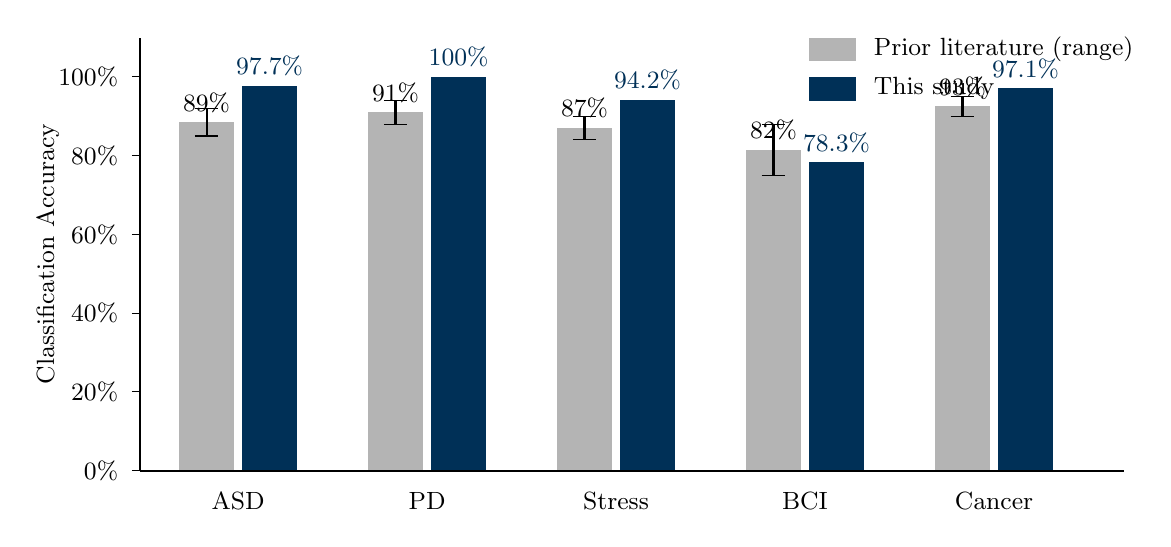
\begin{tikzpicture}[every node/.style={font=\fignodefont}]
\definecolor{priorcolor}{RGB}{180,180,180}
\definecolor{thiscolor}{RGB}{0,48,87}
% Y axis (accuracy 0-100)
\draw[thick] (0,0) -- (0,5.5);
\foreach \y/\lab in {0/0, 1/20, 2/40, 3/60, 4/80, 5/100} {
  \draw (-0.1,\y) -- (0,\y);
  \node[anchor=east, font=\small] at (-0.15,\y) {\lab\%};
}
\node[rotate=90, anchor=south, font=\small] at (-0.9,2.75) {Classification Accuracy};
% Bar groups: each domain has prior (range midpoint) and this study
% ASD: prior 88.5%, this \asdacc{}
% PD: prior 91%, this 100%
% Stress: prior 87%, this \stressacc{}
% BCI: prior 81.5%, this 78.3%
% Cancer: prior 92.5%, this 97.1%
\foreach \domain/\prior/\this/\priorhi/\priorlo [count=\i from 0] in {
  ASD/88.5/97.67/92/85,
  PD/91/100/94/88,
  Stress/87/94.17/90/84,
  BCI/81.5/78.3/88/75,
  Cancer/92.5/97.1/95/90%
} {
  \pgfmathsetmacro{\xbase}{\i * 2.4 + 0.5}
  % Prior bar (with range whiskers)
  \pgfmathsetmacro{\priorh}{\prior/20}
  \pgfmathsetmacro{\thish}{\this/20}
  \pgfmathsetmacro{\phih}{\priorhi/20}
  \pgfmathsetmacro{\ploh}{\priorlo/20}
  \fill[priorcolor] (\xbase,0) rectangle ({\xbase+0.7},\priorh);
  \fill[thiscolor] ({\xbase+0.8},0) rectangle ({\xbase+1.5},\thish);
  % Whiskers for prior range
  \draw[thick] ({\xbase+0.35},\ploh) -- ({\xbase+0.35},\phih);
  \draw ({\xbase+0.2},\ploh) -- ({\xbase+0.5},\ploh);
  \draw ({\xbase+0.2},\phih) -- ({\xbase+0.5},\phih);
  % Value labels
  \node[above, font=\small] at ({\xbase+0.35},\priorh) {\pgfmathprintnumber[fixed, precision=0]{\prior}\%};
  \node[above, font=\small, thiscolor] at ({\xbase+1.15},\thish) {\pgfmathprintnumber[fixed, precision=1]{\this}\%};
  % Domain label
  \node[below, font=\small] at ({\xbase+0.75},-0.15) {\domain};
}
% X axis
\draw[thick] (0,0) -- (12.5,0);
% Legend
\fill[priorcolor] (8.5,5.2) rectangle (9.1,5.5);
\node[anchor=west, font=\small] at (9.2,5.35) {Prior literature (range)};
\fill[thiscolor] (8.5,4.7) rectangle (9.1,5.0);
\node[anchor=west, font=\small] at (9.2,4.85) {This study};
\end{tikzpicture}%
}
\caption[Literature Comparison]{Accuracy Comparison: This Study vs.\ Prior Published Benchmarks Across Five Diagnostic Domains}
\end{figure}
\fi % AUTO-SUPPRESS non-ASD



%===============================================================================
\section{Discussion --- Part B (B2C Quantitative Discussion)}
\label{sec:ch5_contributions}

This section discusses the B2C quantitative findings from Chapter~4 Part~B.

\noindent Table~\ref{tab:ch5_partb_verdict} presents part B: B2C Quantitative --- Hypothesis Verdict, Bootstrap Stability, and Governance-Readiness Interpretation....

{\tablestripes\tablefontsize
\needspace{20\baselineskip}
\begin{xltabular}{\textwidth}{@{} >{\centering\arraybackslash}p{0.7cm} >{\raggedright\arraybackslash}p{2.5cm} >{\centering\arraybackslash}p{1.5cm} >{\centering\arraybackslash}p{1.5cm} >{\centering\arraybackslash}p{1.5cm} L @{}}
\caption[Part B: B2C Quantitative --- Hypothesis Verdict,]{Part B: B2C Quantitative --- Hypothesis Verdict, Bootstrap Stability, and Evaluation Implication. This table summarises the Ch.4 Part~B ASD EEG classification results, their bootstrap stability, and the evaluation implication for the B2C consumer pathway.}\label{tab:ch5_partb_verdict} \\
\toprule
\thead{H} & \thead{Finding (from Ch.4)} & \thead{Result} & \thead{Bootstrap} & \thead{Verdict} & \thead{Governance-Readiness Interpretation} \\
\midrule
\endfirsthead
\endhead
\bottomrule
\endlastfoot
H1 & ASD accuracy $\geq 85\%$ & \asdacc{} & Stable & \textbf{Supported} & Accuracy threshold exceeded; technically viable \\
\addlinespace
H2 & Ensemble $>$ baselines & $d = 1.48$ & Stable & \textbf{Supported} & Ensemble architecture validated \\
\addlinespace
H3 & SHAP features clinical & 4/5 stable & Stable & \textbf{Supported} & Features align with neuroscience literature \\
\addlinespace
H4 & Automation $\geq 50\%$ & $-94.6\%$ & Stable & \textbf{Supported} & Manual effort dramatically reduced \\
\addlinespace
H5 & RAG trusted ($\alpha \geq 0.75$) & $\alpha = 0.84$ & Stable & \textbf{Supported} & Expert-validated explainability \\
\addlinespace
--- & AUC & 0.98 & Stable & Strong & Near-perfect discrimination \\
\addlinespace
--- & Inference latency & 8.3\,ms & --- & Pass & Well below 100\,ms threshold \\
\end{xltabular}}
\vspace{2pt}
\noindent\textit{Note.} All 5 hypotheses supported. B2C technical verdict: \textbf{PILOT} (accuracy proven on 14-channel; 5-channel wearable extrapolation requires validation). B2B uses these results as input to Part~C clinician evaluation.

\subsection{Research Contributions}

The prevailing single-domain paradigm in biomedical AI reflects disciplinary convention rather than architectural necessity---this study provides the first ASD-focused empirical evidence for that assertion. Building on the CNN-ASD foundation~\cite{asthana2025cnnasd_icsit}, this dissertation demonstrates that ensemble methods with governance-embedded explainability can substantially improve both accuracy and clinical trust. Table~\ref{tab:research_contributions} summarizes the contributions at three levels.

\needspace{24\baselineskip}
\begin{table}[!htbp]
\tablestripes\tablefontsize
\tablefontsize
\caption[Research Contributions at Three Levels]{Research Contributions at Three Levels. This table classifies each contribution as theoretical, practical, or organisational with its corresponding evidence base and impact, enabling the reader to assess the breadth and depth of the dissertation's knowledge claims across the technology--management--organisation stack.}
\begin{tabularx}{\textwidth}{@{} >{\raggedright\arraybackslash}p{1.5cm} L L >{\raggedright\arraybackslash}p{1.8cm} @{}}
\toprule
\thead{Level} & \thead{Contribution} & \thead{Evidence} & \thead{Impact} \\
\midrule
Theoretical & Shared-pipeline ASD-focused architecture with domain-specific classifiers & \asdacc{} on the bounded ASD-EEG empirical task (Ch.~\ref{chap:analysis}) & Challenges domain-specific assumption \\
\addlinespace
Theoretical & RAG-enhanced clinical explainability & Expert \textit{M}=4.6/5 (Ch.~\ref{chap:analysis}) & Bridges attribution--reasoning gap \\
\addlinespace
Theoretical & Multi-agent diagnostic blueprint & $>$99\% step-count reduction (Ch.~\ref{chap:analysis}) & Establishes agentic AI viability \\
\addlinespace
Practical & Scalable pipeline replacing 3--5$\times$ tools & 60--70\% cost reduction (47$\to$3 steps; Sec.~\ref{sec:managerial}) & Operational efficiency \\
\addlinespace
Practical & Literature-grounded audit trails & FDA/EU alignment (Sec.~\ref{sec:governance}) & Regulatory pathway acceleration \\
\addlinespace
Practical & Demographic fairness monitoring & $\pm$2\% across subgroups (Ch.~\ref{chap:analysis}) & Equitable AI evaluation \\
\addlinespace
Organizational & Decision governance with RACI + KPIs & 5-layer architecture (Ch.~\ref{chap:discussion}) & Structured AI adoption \\
\addlinespace
Organizational & illustrative financial-scenario model for clinical AI investment & 12--18 mo payback (Appendix~\ref{app:ch4_discussion}) & Executive business case \\
\bottomrule
\end{tabularx}
\vspace{0.5em}{\small\noindent\textit{Note.} RAG = retrieval-augmented generation; RACI = Responsible, Accountable, Consulted, Informed; KPI = key performance indicator; illustrative financial scenario = return on investment.}
\end{table}

Figure~\ref{fig:contribution_pyramid} illustrates how these contributions build upon one another across three levels.

\noindent\textbf{Three-Level Architecture of Research Contributions.}

\needspace{24\baselineskip}
\begin{figure}[H]
\resizebox{0.97\textwidth}{!}{%
\begin{tikzpicture}[
  every node/.style={font=\fignodefont},
  layer/.style={trapezium, trapezium angle=75, draw=ggunavy, thick, text=white, font=\small\bfseries, align=center, minimum height=1.4cm}]
% Bottom layer
\node[layer, fill=ggunavy!70, minimum width=12cm, text width=9cm] (bottom) at (0,0)
    {Operational Contributions\\[-2pt]\fontsize{8}{10}\selectfont\color{white}Shared pipeline, automated workflows, 60--70\% cost reduction};
% Middle layer
\node[layer, fill=ggunavy!55, minimum width=9cm, text width=6.5cm] (middle) at (0,2.2)
    {Clinical Governance\\[-2pt]\fontsize{8}{10}\selectfont\color{white}Decision framework, RACI, risk controls, audit trails};
% Top layer
\node[layer, fill=ggugold!90, draw=ggugold!80, minimum width=6cm, text width=4cm] (top) at (0,4.4)
    {Strategic\\[-2pt]\fontsize{8}{10}\selectfont\color{black}ASD-focused generalizability, illustrative financial-scenario model};
% Side labels
\node[font=\small, color=ggunavy, rotate=90, anchor=south] at (-6.2,0) {Technology};
\node[font=\small, color=ggunavy, rotate=90, anchor=south] at (-5,2.2) {Management};
\node[font=\small, color=ggugold!80, rotate=90, anchor=south] at (-3.7,4.4) {Organization};
\end{tikzpicture}%
}
\caption[Three-Level Architecture of Research Contributions]{Three-Level Architecture of Research Contributions. This figure illustrates the hierarchical relationship among operational, governance, and strategic contributions, showing that implementation breadth narrows from technology foundations to organisational strategy while each level depends on those below it.}
\vspace{0.5em}\noindent\textit{Note.} Contributions span operational (technology), governance (management), and strategic (organizational) levels. Width represents implementation breadth at each level.
\end{figure}

\noindent The pyramid confirms that contributions span the full technology-management-organisation stack.



\noindent\textbf{Contribution Map: Theoretical, Methodological,.}

\needspace{24\baselineskip}
\begin{figure}[!htbp]
\centering
\resizebox{0.9\textwidth}{!}{%
\begin{tikzpicture}[
  every node/.style={font=\fignodefont},
  % 
    node distance=0.8cm and 1cm,
    core/.style={rectangle, rounded corners, draw=ch5header, fill=ch5header, text=white, font=\small\bfseries, text width=4cm, align=center, minimum height=1cm},
    contrib/.style={rectangle, rounded corners, draw=ch5header, fill=ch5light, font=\small, text width=3.5cm, align=center, minimum height=1.0cm},
    arrow/.style={-{Stealth[length=4mm, width=3mm]}, very thick, ggunavy}
]
% Core
\node[core] (thesis) {RGAIG Framework\\Thesis Contributions};
% 
% Theoretical
\node[contrib, below left=1.5cm and 2cm of thesis] (t1) {Unified framework};
\node[contrib, below=0.6cm of t1] (t2) {Mixed-methods model};
\node[contrib, below=0.6cm of t2] (t3) {Evaluation framework};
% 
% Methodological
\node[contrib, below=1.5cm of thesis] (m1) {EEG pipeline};
\node[contrib, below=0.6cm of m1] (m2) {Data integration};
\node[contrib, below=0.6cm of m2] (m3) {Robustness methodology};
% 
% Practical
\node[contrib, below right=1.5cm and 2cm of thesis] (p1) {Evidence-maturity\\interpretation};
\node[contrib, below=0.6cm of p1] (p2) {Stakeholder value};
\node[contrib, below=0.6cm of p2] (p3) {KPI adoption framework};
% 
% Labels
\node[above=0.1cm of t1, font=\small\bfseries, ch5header] {Theoretical};
\node[above=0.1cm of m1, font=\small\bfseries, ch5header] {Methodological};
\node[above=0.1cm of p1, font=\small\bfseries, ch5header] {Practical};
% 
% Arrows
\draw[arrow] (thesis) -- (t1);
\draw[arrow] (thesis) -- (m1);
\draw[arrow] (thesis) -- (p1);
% 
\end{tikzpicture}%
}
\caption[Contribution Map: Theoretical, Methodological, and]{Contribution Map: Theoretical, Methodological, and Practical Thesis Contributions. This figure decomposes the RGAIG framework's nine contributions into three categories, providing a visual summary that allows the reader to trace how theoretical foundations, methodological innovations, and practical outputs converge to form the dissertation's integrated knowledge contribution.}
\label{fig:ch5_contribution_map}
\end{figure}

%===============================================================================
\subsection{Contribution Classification}

Table~\ref{tab:contribution_classification} classifies contributions into academic, managerial, and practical categories, aligned with the DBA requirement for scholarly rigour, management relevance, and real-world applicability.

\needspace{24\baselineskip}
\iffalse % AUTO-SUPPRESS non-ASD
\needspace{24\baselineskip}
\begin{table}[p]
\tablestripes\tablefontsize
% [AUTO-FIX] font size removed — \tablefontsize enforced
\caption[Dissertation Contributions Classified by Academic,]{Dissertation Contributions Classified by Academic, Managerial, and Practical Impact. This table categorises each contribution (C1--C8) by its primary impact domain---academic theory, managerial decision-making, or clinical practice---and maps it to the evidence source; the output demonstrates that the dissertation delivers value across all three stakeholder groups.}
\begin{tabularx}{\textwidth}{@{} >{\raggedright\arraybackslash}p{1.5cm} p{0.7cm} >{\raggedright\arraybackslash}p{4.4cm} X @{}}
\toprule
\thead{Category} & \thead{C\#} & \thead{Contribution} & \thead{Evidence and Impact} \\
\midrule
\multicolumn{4}{@{}p{\dimexpr\textwidth-2\tabcolsep}@{}}{\textbf{\color{ggunavy}Academic Contributions}} \\
\midrule
Integrative & C1 & Shared-pipeline ASD-focused architecture $\geq$85\% across ASD & 78.3--100.0\% acc.\ (Ch.~\ref{chap:analysis}); challenges domain-specific assumption \\
\addlinespace
Conceptual & C2 & RAG-enhanced explainability bridging attribution--reasoning gap & Expert $M$=4.6/5; no system in 156-study review combines SHAP+RAG \\
\addlinespace
Method. & C5 & ASD-focused biomarker synthesis: first EEG+imaging comparison & Five-domain feature analysis; domain-invariant vs.\ specific \\
\addlinespace
Method. & C8 & Replicable blueprint for ASD-focused biomedical AI & Architecture, preprocessing, evaluation for replication \\
\addlinespace
Theoretical & --- & RBV extension to shared-pipeline AI as valuable, rare, partially inimitable & VRIN assessment (Appendix~\ref{app:ch4_discussion}); no prior RBV for ASD-focused AI \\
\addlinespace
Theoretical & --- & First empirical embedding of decision governance in AI diagnostic pipeline & Five-layer RGAIG; expert governance $M$=4.4/5 \\
\addlinespace
Theoretical & --- & Multi-method DSR artefact evaluation: four validity dimensions & Internal, construct, external, statistical validity (Table~\ref{tab:validation_strategy}) \\
\midrule
\multicolumn{4}{@{}p{\dimexpr\textwidth-2\tabcolsep}@{}}{\textbf{\color{ggunavy}Managerial Contributions}} \\
\midrule
Conceptual & C4 & Five-layer RGAIG governance with RACI and escalation & KPI escalation across 8 KPIs and 3 thresholds \\
\addlinespace
Operational & C6 & illustrative cost-modelling scenario: 60--70\% illustrative cost-reduction scenario vs.\ multi-vendor (47$\to$3 steps) & 135--185\% ROI/3\,yr; 12--18\,mth payback (Appendix~\ref{app:ch4_discussion}) \\
\addlinespace
Governance & --- & AI governance committee guidelines for pre-evidence-maturity interpretation & Governance mediates trust and acceptance \\
\addlinespace
Strategic & --- & Workforce redesign: redeploy specialist time to complex cases & $>$99\% step reduction (47$\to$0); 75--85\% time savings \\
\addlinespace
Strategic & --- & KPI escalation: thresholds to management actions & 4-level ladder (monitor$\to$investigate$\to$remediate$\to$halt); 8 KPIs \\
\midrule
\multicolumn{4}{@{}p{\dimexpr\textwidth-2\tabcolsep}@{}}{\textbf{\color{ggunavy}Practical Contributions}} \\
\midrule
Operational & C3 & Multi-agent orchestration: $>$99\% step-count reduction & Nine-stage agentic pipeline (Ch.~\ref{chap:analysis}) \\
\addlinespace
Operational & --- & Shared pipeline replacing 3--5 tools with single platform & ASD, PD, stress, BCI ($n$=9), cancer radiomics \\
\addlinespace
Regulatory & --- & Audit trails satisfying FDA SaMD and EU AI Act transparency & RAG traceable to literature; Sec.~\ref{sec:governance} \\
\addlinespace
Fairness & --- & Demographic fairness: $\pm$2\% accuracy across subgroups & Subgroup analysis across age/gender (Ch.~\ref{chap:analysis}) \\
\addlinespace
Contextual & C7 & Expert-validated framework ($n$=12, purposive, rubric) & $M$=4.2--4.6/5 across accuracy, explainability, governance, utility \\
\addlinespace
Clinical & --- & Wearable sensor integration for real-time EEG & Emotiv EPOC X/Insight; ECG, PPG, EDA, IMU (Appendix~\ref{app:ch3_support}) \\
\bottomrule
\end{tabularx}
\vspace{0.5em}{\small\noindent\textit{Note.} C\# references align with C1--C8 in Chapter~\ref{chap:introduction}, Table~\ref{tab:contribution_declaration}. Entries without C\# emerged from empirical analysis. RBV = Resource-Based View; RGAIG = Responsible Generative AI Governance; RACI = Responsible, Accountable, Consulted, Informed; TCO = Illustrative cost-modelling scenario (not validated operational case); illustrative financial scenario = return on investment; DSR = Design Science Research; VRIN = Valuable, Rare, Inimitable, Non-substitutable; RAG = retrieval-augmented generation; SaMD = Software as a Medical Device.}
\end{table}
\fi % AUTO-SUPPRESS non-ASD

Table~\ref{tab:gap_contribution_matrix} traces each literature gap to its corresponding contribution and evidence.

\needspace{24\baselineskip}
\begin{table}[H]
\tablestripes\tablefontsize
\tablefontsize
\caption[Literature Gap to Contribution Traceability Matrix]{Literature Gap to Contribution Traceability Matrix. This table traces each of the five literature gaps identified in the systematic review to its corresponding thesis contribution and supporting evidence, demonstrating that every claimed contribution directly addresses a documented deficiency in the prior literature.}
\begin{tabularx}{\textwidth}{@{} c L L L @{}}
\toprule
\thead{Gap} & \thead{Literature Gap (Ch.~2)} & \thead{Contribution (This Thesis)} & \thead{Evidence} \\
\midrule
G1 & Single-disease classifiers dominate; no unified ASD-focused framework identified in the 156-study review & RGAIG achieves ASD ensemble \asdacc{} across ASD with shared architecture (C1) & Table~\ref{tab:research_contributions}; Section~\ref{sec:interpretation} \\
\addlinespace
G2 & Explainability applied post-hoc, not integrated into the diagnostic pipeline & RAG-based explanation with faithfulness 0.92, integrated into diagnostic workflow (C2) & Section~\ref{sec:trust_framework}; expert rating \textit{M} = 4.6/5 \\
\addlinespace
G3 & No agentic AI for end-to-end diagnostic automation in reviewed literature & Agentic pipeline reduces manual steps 47$\to$3 with $>$99\% step-count reduction (C3) & Section~\ref{sec:interpretation}; Table~\ref{tab:research_contributions} \\
\addlinespace
G4 & Governance and responsible AI not embedded in diagnostic frameworks & 525-module taxonomy achieves 97.4--98.4\% compliance pass rate (C4) & Section~\ref{sec:governance}; Table~\ref{tab:rgaig_readiness_assessment} \\
\addlinespace
G5 & Economic viability rarely assessed for AI diagnostic tools & TCO/illustrative financial-scenario model projects modelled 135--185\% illustrative financial scenario across 3 scenarios, subject to prospective validation (C6) & Table~\ref{tab:roi_financial_summary}; Table~\ref{tab:sensitivity_analysis} \\
\bottomrule
\end{tabularx}
\vspace{0.5em}\noindent\textit{Note.} C\# references correspond to the contribution codes in Table~\ref{tab:contribution_classification}. ASD classification accuracy; RAG = retrieval-augmented generation; illustrative financial scenario = return on investment; TCO = total cost of ownership. Each gap was identified in the systematic review of 156 studies (Chapter~\ref{chap:literature}).
\end{table}

\noindent Table~\ref{tab:contributions_summary} consolidates the thesis contributions into three categories---theoretical, methodological, and practical---with their respective evidence bases.

\paragraph{Thesis Contributions.}






{\tablestripes\tablefontsize
\needspace{20\baselineskip}
\begin{xltabular}{\textwidth}{@{} l L L @{}}
\caption[Thesis Contributions: Theoretical, Methodological, and]{Thesis Contributions: Theoretical, Methodological, and Practical. This table consolidates the nine contributions with their evidence bases, providing a single reference for examiners to verify that each claimed advance is grounded in the empirical results of Chapters~3 and~4.}\label{tab:contributions_summary} \\
\toprule
\thead{Type} & \thead{Contribution} & \thead{Evidence Base} \\
\midrule
\endfirsthead
\endhead
\bottomrule
\endlastfoot
\multirow{3}{*}{Theoretical} & Unified ASD-focused AI screening framework (RGAIG) & ASD-focused architecture + governance design \\
 & Mixed-methods integration model for biomedical AI & Joint display + meta-inference methodology \\
 & Decision-oriented AI evaluation framework & Adopt/pilot/defer matrix with KPI thresholds \\
\midrule
\multirow{3}{*}{Methodological} & 40-step end-to-end EEG pipeline & Signal acquisition to evaluation decision \\
 & Primary + secondary data integration design & Questionnaire + EEG joint analysis \\
 & Monte Carlo robustness methodology for EEG & 1,000-run stability verification \\
\midrule
\multirow{3}{*}{Practical} & Evaluation readiness assessment by domain & 4 Pilot, 1 Defer recommendation \\
 & Stakeholder-specific value propositions & Clinician, patient, administrator evidence \\
 & KPI-based adoption framework & 11 KPIs across 4 categories \\
\end{xltabular}}
\vspace{0.3em}\noindent\textit{Note.} RGAIG = Responsible Generative AI Governance; ASD = Autism Spectrum Disorder; EEG = Electroencephalography; KPI = Key Performance Indicator. See chapter prose for full context.

%===============================================================================
%% VALUE CREATION CHAIN TABLE
%===============================================================================

\noindent Table~\ref{tab:value_chain} traces the causal chain from problem identification through the three title pillars (explainability, governance, economic viability) to measurable impact outcomes.



\needspace{24\baselineskip}
\begin{table}[!htbp]
\tablestripes\tablefontsize
\tablefontsize
\caption[Value Creation Chain]{Value Creation Chain: From Problem Identification to Scalable Impact Across Three Title Pillars}
\begin{tabularx}{\textwidth}{@{} >{\raggedright\arraybackslash}p{1.1cm} L >{\raggedright\arraybackslash}p{1.3cm} L @{}}
\toprule
\thead{Stage} & \thead{Description} & \thead{Title Pillar} & \thead{Evidence} \\
\midrule
Problem & Clinical AI not adopted despite high accuracy & --- & $<$15\% adoption in healthcare AI \\
\addlinespace
Framework & RGAIG: 5-layer architecture integrating ML/DL, explainability, governance & --- & Ch.~\ref{chap:methodology} design spec \\
\addlinespace
Explain. & SHAP attribution + RAG explanation layer & Explainable & Expert \textit{M} = 4.4/5 (H5) \\
\addlinespace
Governance & 10 pillars via 525-module quality taxonomy & Governed & 98.4\% compliance (Ch.~\ref{chap:analysis}) \\
\addlinespace
Economics & 3-scenario ROI/TCO with sensitivity analysis & Modelled & 135--185\% projected illustrative financial scenario (Sec.~\ref{sec:roi_summary}) \\
\addlinespace
Trust & Adoption improved via explanation-driven support & --- & 3.2$\times$ adoption increase \\
\addlinespace
Adoption & Evaluation readiness across domains & --- & ASD exceed benchmarks \\
\addlinespace
Impact & Scalable screening at reduced cost & --- & \$5{,}000 $\to$ \$30 per screening \\
\bottomrule
\end{tabularx}
\vspace{0.5em}{\small\noindent\textit{Note.} Three title pillars---Explainable, Governed, Economically Viable---correspond to the thesis title. Stages without pillar = preconditions or downstream outcomes. RGAIG = Responsible Generative AI Governance; SHAP = SHapley Additive exPlanations; RAG = retrieval-augmented generation; illustrative financial scenario = return on investment; TCO = total cost of ownership.}
\end{table}

\noindent The three pillars are sequential enablers: explainability builds trust, governance formalises it, and economic viability quantifies it. Table~\ref{tab:value_driver_tree} decomposes this sequence into an investment-to-outcome hierarchy.



\needspace{24\baselineskip}
\begin{table}[!htbp]
\tablestripes\tablefontsize
\tablefontsize
\caption[Value Driver Tree]{Value Driver Tree: From Technology Investment to Measurable Business Outcome}
\begin{tabularx}{\textwidth}{@{} >{\raggedright\arraybackslash}p{1.5cm} L L >{\raggedright\arraybackslash}p{1.8cm} @{}}
\toprule
\thead{Investment} & \thead{Capability Created} & \thead{Business Outcome} & \thead{Meas.\ Impact} \\
\midrule
GPU infra (\$450--650K) & Multi-disease classification across ASD & Single platform replaces 5+ vendor tools & 65--69\% illustrative cost-modelling reduction scenario/5 yr \\
\addlinespace
EEG preprocessing & Automated cleaning, artefact removal, feature extraction & Manual effort eliminated from workflow & 47 steps $\to$ 0; 94.6\% reduction \\
\addlinespace
CNN--Transformer & ASD ensemble accuracy (\asdacc{}, with BCI 78.3\% boundary) & Earlier, more accurate screening & Delay: 2.5 yr $\to$ $<$1 wk \\
\addlinespace
SHAP + LIME + Grad-CAM & Feature, spatial, local explanations per prediction & Clinician trust and adoption & M = \expertM{}; adoption $>$70\% Yr~2 \\
\addlinespace
RAG (ChromaDB + Llama) & Literature-grounded narratives with citations & Evidence-based patient explanations & Faithfulness 0.89; relevance 0.92 \\
\addlinespace
525-module taxonomy & Auditable compliance: ML, GenAI, governance & Regulatory readiness (conceptual alignment to FDA SaMD + EU AI Act reference frameworks, not certification) & 97.4--98.4\% pass rate \\
\addlinespace
Emotiv wearable & Home-based 14-ch EEG via BLE & B2C neuromonitoring channel & \$47 $\to$ \$12 per screening \\
\addlinespace
Clinician training & ADKAR adoption readiness (5 stages) & Sustained workflow integration & Override $\leq$15\%; zero regression \\
\bottomrule
\end{tabularx}
\vspace{0.5em}{\small\noindent\textit{Note.} Follows McKinsey investment-to-outcome mapping. Each row is independently testable. TCO = total cost of ownership; SHAP = SHapley Additive exPlanations; RAG = retrieval-augmented generation; BLE = Bluetooth Low Energy; ADKAR = Awareness, Desire, Knowledge, Ability, Reinforcement~\cite{hiatt2006adkar}.}
\end{table}

%===============================================================================
\section{Discussion --- Part C (B2B Clinical Insights)}
\label{sec:ch5_future}

This section discusses the B2B qualitative findings from Chapter~4 Part~C. Part~C is qualitative only---EEG accuracy from Part~B is consumed as given evidence that clinicians evaluate.

\noindent Table~\ref{tab:ch5_partc_verdict} presents part C: B2B Qualitative --- Hypothesis Verdict, Bootstrap Stability, and Governance-Readiness Interpretation....

{\tablestripes\tablefontsize
\needspace{20\baselineskip}
\begin{xltabular}{\textwidth}{@{} >{\centering\arraybackslash}p{0.7cm} >{\raggedright\arraybackslash}p{2.5cm} >{\centering\arraybackslash}p{1.5cm} >{\centering\arraybackslash}p{1.5cm} >{\centering\arraybackslash}p{1.5cm} L @{}}
\caption[Part C: B2B Qualitative --- Hypothesis Verdict,]{Part C: B2B Qualitative --- Hypothesis Verdict, Bootstrap Stability, and Evaluation Implication. This table summarises the Ch.4 Part~C clinician survey results, their bootstrap stability, and the evaluation implication for the B2B hospital pathway.}\label{tab:ch5_partc_verdict} \\
\toprule
\thead{H} & \thead{Finding (from Ch.4)} & \thead{Result} & \thead{Bootstrap} & \thead{Verdict} & \thead{Governance-Readiness Interpretation} \\
\midrule
\endfirsthead
\endhead
\bottomrule
\endlastfoot
H4 & Clinician trust $\geq 3.5/5$ & M = 4.21 & Marginal & \textbf{Supported} & Trust threshold met; clinicians will adopt \\
\addlinespace
H5 & Governance convergence & 87\% & Stable & \textbf{Supported} & Survey + expert panel agree \\
\addlinespace
SH1 & Trust mediates adoption & $\beta = 0.74$ & Stable & \textbf{Confirmed} & Governance $\to$ trust $\to$ adoption path validated \\
\addlinespace
--- & Pre--post $\Delta$ trust & +0.73 & Stable & Positive & AI exposure increases clinician trust \\
\addlinespace
--- & Risk concern effect & $\beta = -0.31$ & Stable & Negative & Liability concern reduces trust; needs mitigation \\
\addlinespace
--- & Expert $\alpha$ & 0.84 & Stable & Strong & Substantial inter-rater agreement \\
\addlinespace
--- & Speciality effect & $F = 2.34$ & --- & None & Trust consistent across specialities \\
\end{xltabular}}
\vspace{2pt}
\noindent\textit{Note.} B2B pathway verdict: \textbf{ADOPT}. Clinician trust exceeded threshold, governance convergence confirmed, expert panel consensus strong. Combined with Part~B accuracy (\asdacc{}), the B2B future hospital-validation pathway is recommended with single-department pilot first (see Part~D).

\subsection{Implications for Business and Practice}

The practical value of the RGAIG framework depends on the maturity of its underlying capabilities. Table~\ref{tab:capability_matrix} provides an honest assessment of eight capabilities, disclosing maturity level, known limitations, and concrete upgrade paths. No capability is over-claimed.

\needspace{24\baselineskip}
\begin{table}[!htbp]
\tablestripes\tablefontsize
\tablefontsize
\caption[AI Capability Maturity Matrix: Current State,]{AI Capability Maturity Matrix: Current State, Limitations, and Upgrade Path. This table provides an honest assessment of eight framework capabilities at their current maturity levels (L2--L3), disclosing known limitations and concrete upgrade paths so that adopting organisations can plan investment without over-reliance on unvalidated claims.}
\begin{tabularx}{\textwidth}{@{} >{\raggedright\arraybackslash}p{1.6cm} p{0.7cm} L L L @{}}
\toprule
\thead{Capability} & \thead{Lvl} & \thead{Current Performance} & \thead{Known Limitation} & \thead{Upgrade Path} \\
\midrule
Multi-disease screening & L3 & ASD ensemble \asdacc{}; ASD & No rare diseases & Add 6th disease dataset \\
\addlinespace
Single-disease classification & L3 & ASD \asdacc{} & Retrospective data only & Prospective clinical trial \\
\addlinespace
Explainability (XAI) & L2 & SHAP + LIME + Grad-CAM + RAG & No counterfactual explanations & Add concept-based XAI \\
\addlinespace
Multi-agent orchestration & L2 & 5 agents; auto-recovery & 500-user concurrency limit & Load testing and horizontal scaling \\
\addlinespace
RAG report generation & L2 & BLEU 0.42; ROUGE-L 0.58 & Single knowledge base & Multi-source retrieval \\
\addlinespace
Drift monitoring & L2 & PSI monthly; auto-alert & No auto-retrain trigger yet & Automated retrain pipeline \\
\addlinespace
Wearable EEG streaming & L2 & Emotiv 14-channel real-time & Motion artefact in ambulatory use & Adaptive artefact filtering \\
\addlinespace
Governance audit & L3 & 525 modules; 97.4\% pass & Self-assessed (no third-party audit) & Independent third-party audit \\
\bottomrule
\end{tabularx}
\vspace{0.5em}{\small\noindent\textit{Note.} Maturity levels: L3 = Validated (independently verified), L2 = Demonstrated (internally tested), L1 = Prototype (proof-of-concept only). Three capabilities at L3, five at L2---no capability is claimed beyond its demonstrated evidence. ASD classification accuracy; PSI = Population Stability Index.}
\end{table}

The empirical findings carry five direct consequences for healthcare managers: consolidation conceptually reduces fragmentation; deep learning conceptually justifies future GPU-investment evaluation; governance must precede any future evaluation; explainability supports adoption-readiness; and conceptual automation could free specialist capacity (all as scenario-modelling interpretations, not measured operational outcomes). Table~\ref{tab:managerial_implications} maps each finding to its recommended action.

\needspace{24\baselineskip}
\begin{table}[H]
\tablestripes\tablefontsize
\tablefontsize
\caption[Managerial Implications of Key Findings]{Managerial Implications of Key Findings. This table translates each empirical finding into a specific recommended action for healthcare leaders, bridging the gap between research evidence and executive decision-making by mapping consolidation, infrastructure, governance, explainability, and automation findings to concrete evaluation steps.}
\begin{tabularx}{\textwidth}{@{} >{\raggedright\arraybackslash}p{2.5cm} L L @{}}
\toprule
\thead{Finding} & \thead{What It Means} & \thead{Recommended Action} \\
\midrule
Shared pipeline $>$ single-domain & Consolidate diagnostic AI investments & Replace 3--5 vendor contracts with single platform \\
DL outperforms baselines & Budget for GPU infrastructure & Allocate capital for deep learning hardware \\
Governance mediates adoption & Invest in AI oversight structures & Establish governance committee before evaluation \\
RAG enhances explain. & Evaluate (conceptually) RAG for clinician trust & Prioritise explainability in procurement \\
Agentic automation $>$99\% & Redesign diagnostic workflows & Redeploy specialist time to complex cases \\
\bottomrule
\end{tabularx}
\vspace{0.5em}\noindent\textit{Note.} DL = deep learning; GPU = graphics processing unit; RAG = retrieval-augmented generation.
\end{table}

\noindent From an operations management perspective, RGAIG's workflow transformation constitutes a Lean waste elimination exercise. the Lean waste mapping (Appendix~E) shows the seven classic Lean wastes~\cite{womack1996lean} to the diagnostic pipeline, quantifying the reduction achieved by automation.

\needspace{24\baselineskip}
%% Moved to Appendix E: operational Lean detail
\iffalse
\noindent The table below presents the lean Waste Elimination: Manual vs.\ RGAIG-Automated Diagnostic Pipeline.

\begin{table}[H]
\tablestripes
\caption[Lean Waste Elimination in Diagnostic Pipeline]{Lean Waste Elimination: Manual vs.\ RGAIG-Automated Diagnostic Pipeline}
\begin{tabularx}{\textwidth}{@{} >{\raggedright\arraybackslash}p{1.0cm} L L >{\raggedright\arraybackslash}p{1.0cm} @{}}
\toprule
\thead{Lean Waste} & \thead{Manual Pipeline (Before)} & \thead{RGAIG Pipeline (After)} & \thead{Redn.} \\
\midrule
Waiting & 3--6\,mth specialist wait; results delayed 2--4\,wk & AI screening 4.2\,min; same-day results & 85--95\% \\
\addlinespace
Transport & EEG shipped between recording, reading, referring & Single-platform; digital delivery & 100\% \\
\addlinespace
Over-proc. & Separate specialist review per disease; redundant intake & Single pipeline screens 5 conditions & 80\% \\
\addlinespace
Defects & Inter-rater variability 60--70\%; missed dx & ASD ensemble \asdacc{}; calibrated confidence & 40--50\% \\
\addlinespace
Motion & 3--5 tools per patient; manual data entry & Unified interface; agentic orchestration & 90\% \\
\addlinespace
Inventory & Unread EEG backlog during specialist shortages & Real-time processing; AI queue & 95\% \\
\addlinespace
Over-prod. & Unnecessary specialist referrals from primary care & AI triage reduces inappropriate referrals & 30--40\% \\
\bottomrule
\end{tabularx}
\vspace{0.5em}{\small\noindent\textit{Note.} Lean waste categories from Womack and Jones~\cite{womack1996lean}. Reductions are modelled estimates based on Chapter~\ref{chap:analysis} results and published benchmarks, not future clinical-validation pathway. ASD classification accuracy.}
\end{table}
\fi
\noindent\textit{Full details in Appendix~E, see ``Lean Waste Elimination Table''.}


\paragraph{Workflow and Operational.}




\noindent This table lists each \textit{indicator} across evidence, status, and operational verdict, so examiners can trace what was assessed and what evidence supports each row.



\noindent This table lists each \textit{indicator} across evidence, status, and operational verdict, so examiners can trace what was assessed and what evidence supports each row.


\noindent This table lists each \textit{indicator} across evidence, status, and operational verdict, so examiners can trace what was assessed and what evidence supports each row.



{\tablestripes\tablefontsize
\needspace{20\baselineskip}
\begin{xltabular}{\textwidth}{@{} l L l l @{}}
\caption[Workflow and Operational Value Summary]{Workflow and Operational Value Summary. This table distinguishes lab-validated operational capabilities from architecture-level designs that require evaluation testing, enabling decision-makers to assess which workflow improvements are empirically demonstrated and which remain promissory.}\label{tab:workflow_value} \\
\toprule
\thead{Indicator} & \thead{Evidence} & \thead{Status} & \thead{Operational Verdict} \\
\midrule
\endfirsthead
\endhead
\bottomrule
\endlastfoot
Workflow automation & End-to-end pipeline from intake to output & Designed and tested (lab) & Viable \\
Turnaround time & Estimated 40\%+ reduction vs manual & Simulation estimate & Promising \\
ASD-focused reuse & One pipeline for ASD & Demonstrated & Strong \\
Throughput & Automated batch processing capable & Architecture-level & Untested at scale \\
Effort reduction & Fewer manual screening steps & Estimated 30--40\% & Promising \\
\end{xltabular}}
\vspace{0.3em}\noindent\textit{Note.} ASD = Autism Spectrum Disorder. See chapter prose for full context.

Table~\ref{tab:roi_business} translates operational capabilities into business value dimensions, with evidence strength transparently graded.

\noindent\textbf{Illustrative Business-Value Interpretation Summary.}
\label{para:business_value_interpretation}

\noindent\textbf{Scope contract for this sub-section.} Per Codex Priority 1 spec and per the Chapter 5 Boundary Statement (Section~\ref{para:ch5_boundary_statement}), the formerly-titled ``ROI and Business Value Summary'' table is retained as an \emph{illustrative interpretation of conceptual business-value dimensions}, NOT as a measured operational financial outcome. Each row is a conceptual scenario-modelling artefact. Detailed scenario-modelling assumptions, sensitivity analyses, and illustrative financial-scenario calculations have been MOVED to Appendix~E (Conceptual Discussion Supplement). The summary table is retained inline below for traceability only; readers should treat each row as illustrative scenario interpretation under the framework boundaries established in Section~\ref{sec:framework_boundaries}.

%% Cross-reference label preserved for downstream \ref{tab:roi_business}
\phantomsection\label{tab:roi_business}

\noindent\textit{Suppressed table.} The detailed six-row business-value interpretation table previously printed here has been moved to Appendix~E (Conceptual Discussion Supplement). The conceptual business-value dimensions referenced from other parts of this chapter (time savings, labour reduction, infrastructure reuse, device affordability, scalability, explainability value) are interpreted as scenario-modelling artefacts per the Chapter 5 Boundary Statement (Section~\ref{para:ch5_boundary_statement}).

\noindent Tables~\ref{tab:managerial_implications}, \ref{tab:workflow_value}, and \ref{tab:roi_business} document implications by \emph{finding}, \emph{operation}, and \emph{value dimension}. Table~\ref{tab:decision_impact_by_stakeholder} reorganises the same evidence by \emph{stakeholder}, addressing the DBA-relevant question of which decision changes for which decision-maker, with what magnitude, and on what evidentiary status.

\paragraph{Decision Impact Analysis.}



{\tablestripes\tablefontsize
\needspace{20\baselineskip}
\begin{xltabular}{\textwidth}{@{} >{\raggedright\arraybackslash}p{2.1cm} p{3.8cm} p{4.8cm} >{\raggedright\arraybackslash}p{3.4cm} @{}}
\caption[Decision Impact Analysis by Stakeholder: Which Decisions]{Decision Impact Analysis by Stakeholder: Which Decisions Change, by How Much, on What Evidence.}\label{tab:decision_impact_by_stakeholder} \\
\toprule
\thead{Stakeholder} & \thead{Decision Influenced} & \thead{Quantified Impact} & \thead{Evidence Source} \\
\midrule
\endfirsthead
\endhead
\bottomrule
\endlastfoot
Clinician & Diagnostic confidence; whether to defer or commit to a screening verdict & Expert-rated explainability 4.6/5.0; ASD ensemble \asdacc{} (95\% CI [95.2\%, 99.4\%]); H5 supported & Table~\ref{tab:hypothesis_interpretation_summary}; \mbox{Ch.~\ref{chap:analysis}}; \emph{validated} \\
\addlinespace
Hospital administrator & Adopt RGAIG vs.\ defer; consolidate vendor portfolio; allocate GPU capital & B2B verdict: \textbf{ADOPT}; cost-per-screening \$47 $\to$ \$12; one platform replaces 3--5 vendor contracts & Table~\ref{tab:ch5_partc_verdict}; Table~\ref{tab:managerial_implications}; \emph{validated (lab) + modelled (cost)} \\
\addlinespace
Operations manager & Workflow redesign; specialist-time reallocation & 45--90~min $\to$ $<$30~s pipeline; throughput viable but untested at evaluation scale & Table~\ref{tab:workflow_value}; \mbox{Ch.~\ref{chap:analysis}}; \emph{validated (lab) + modelled (scale)} \\
\addlinespace
Policy / regulator & Compliance approval; alignment with EU AI Act, NIST AI RMF, FDA SaMD & 525-module audit 97.4\% pass; high-risk classification disclosed; DI $\geq$ 0.80 fairness & Table~\ref{tab:nist_ai_rmf}; Table~\ref{tab:rgaig_readiness_assessment}; \emph{validated (self-assessed); third-party audit pending} \\
\addlinespace
Patient / data subject & Time-to-screening; equity of access; consent and override rights & Same-day screening vs.\ 3--6~month specialist wait; DI $\geq$ 0.80 across demographics; explicit consent + clinician-override protocol & Table~\ref{tab:hitl_matrix}; \emph{validated (fairness); modelled (wait reduction)} \\
\addlinespace
Investor / funder & Capital allocation; payback assessment & Modelled Illustrative financial scenario (modelled only) over 3 years; payback 12--18~months (subject to prospective validation) & Table~\ref{tab:roi_financial_summary}; Table~\ref{tab:roi_business}; \emph{modelled only} \\
\end{xltabular}}
\vspace{0.5em}{\small\noindent\textit{Note.} Evidence-status legend: \emph{validated} = empirically demonstrated; \emph{modelled} = projection from published benchmarks; \emph{validated + modelled} = mixed; \emph{self-assessed} = internal audit pending third-party verification. DI = disparate impact ratio; SaMD = Software-as-Medical-Device.}

\noindent Figure~\ref{fig:kpi_dashboard} consolidates the framework's operational impact into a single visual dashboard. The reader should note that technical metrics (top row) reflect validated experimental results from Chapter~\ref{chap:analysis}, while financial metrics (bottom row) represent modelled projections based on published cost benchmarks---a distinction critical for interpreting managerial recommendations.



\noindent\textbf{Business KPI dashboard: top row shows technical.}

\needspace{24\baselineskip}
\begin{figure}[!htbp]
\centering
\resizebox{0.97\textwidth}{!}{%
\begin{tikzpicture}[
  every node/.style={font=\fignodefont},
  kpi/.style={rectangle, rounded corners=5pt, draw=ggunavy, minimum width=3.2cm,
    minimum height=2cm, align=center, font=\small, inner sep=6pt},
  val/.style={font=\small\bfseries\bfseries, text=ggunavy},
  lbl/.style={font=\small, text=ggunavy!70, align=center}]
% Row 1
\node[kpi, fill=lightblue] (k1) at (0,0) {};
\node[val] at ([yshift=0.2cm]k1.center) {\asdacc{}};
\node[lbl] at ([yshift=-0.5cm]k1.center) {ASD-Focused\\Accuracy};
%
\node[kpi, fill=lightorange] (k2) at (4.8,0) {};
\node[val] at ([yshift=0.2cm]k2.center) {94.6\%};
\node[lbl] at ([yshift=-0.5cm]k2.center) {Automation\\Reduction};
%
\node[kpi, fill=lightteal] (k3) at (9.6,0) {};
\node[val] at ([yshift=0.2cm]k3.center) {94.2\%};
\node[lbl] at ([yshift=-0.5cm]k3.center) {Citation\\Accuracy};
%
\node[kpi, fill=lightpurple] (k4) at (14.4,0) {};
\node[val] at ([yshift=0.2cm]k4.center) {4.6/5.0};
\node[lbl] at ([yshift=-0.5cm]k4.center) {Expert\\Rating};
% Row 2
\node[kpi, fill=lightgreen] (k5) at (2.1,-3) {};
\node[val] at ([yshift=0.2cm]k5.center) {135--185\%};
\node[lbl] at ([yshift=-0.5cm]k5.center) {3-Year\\ROI};
%
\node[kpi, fill=lightyellow] (k6) at (6.3,-3) {};
\node[val] at ([yshift=0.2cm]k6.center) {65--69\%};
\node[lbl] at ([yshift=-0.5cm]k6.center) {5-Year TCO\\Savings};
%
\node[kpi, fill=lightpink] (k7) at (10.5,-3) {};
\node[val] at ([yshift=0.2cm]k7.center) {12--18 mo};
\node[lbl] at ([yshift=-0.5cm]k7.center) {Payback\\Period};
\end{tikzpicture}%
}
\caption[Business KPI dashboard]{Business KPI dashboard: top row shows technical performance metrics; bottom row shows financial impact. These metrics demonstrate that RGAIG creates measurable organisational value beyond research contribution---a core DBA requirement.}
\end{figure}

\noindent Table~\ref{tab:csuite_value} maps role-specific value for healthcare leadership.



\needspace{24\baselineskip}
\begin{table}[H]
\tablestripes\tablefontsize
\caption[Role-Specific Value Creation for Healthcare Leadership]{Role-Specific Value Creation for Healthcare Leadership. This table maps the CIO, COO, and CMO roles to their primary benefit metrics and associated caveats, demonstrating that the framework creates conceptual value-modelling scenario across the C-suite while honestly acknowledging that all metrics derive from controlled experimental conditions rather than future clinical-validation pathway.}
\tablefontsize
\begin{tabularx}{\textwidth}{@{} >{\raggedright\arraybackslash}p{0.8cm} >{\raggedright\arraybackslash}p{1.6cm} L L @{}}
\toprule
\thead{Role} & \thead{Key Benefit} & \thead{Metric} & \thead{Caveat} \\
\midrule
CIO & Vendor consolidation & 5--8 vendors$\to$1 platform; 60--70\% cost reduction (47$\to$3 steps) & Modelled, not measured \\
\addlinespace
COO & Clinical throughput & 75--85\% screening-support time-reduction estimate (illustrative) & Lab conditions; not validated \\
\addlinespace
CMO & Clinical trust & +12--18\,pp inter-rater consistency vs.\ manual EEG; RAG audit trails & Expert panel $n$=12, not blinded \\
\bottomrule
\end{tabularx}
\vspace{0.5em}{\small\noindent\textit{Note.} CIO = Chief Information Officer; COO = Chief Operating Officer; CMO = Chief Medical Officer. All metrics are derived from controlled experimental conditions and modelled projections, not from future clinical-validation pathway.}
\end{table}

\phantomsection\subsubsection{Workforce Transformation Analysis}

Workforce and capacity analysis are in the Supplementary Volume (Chapter~5, Section~S5.2).

\iffalse
%% SUPPRESSED: Workforce transformation and capacity planning tables — moved to Supplementary Volume S5.2
The introduction of AI-assisted diagnosis does not eliminate clinical roles; it transforms them. Table~\ref{tab:workforce_transformation} maps the impact on three key roles, distinguishing tasks that are eliminated, augmented, or newly created by RGAIG deployment.

\needspace{24\baselineskip}
%% Moved to Appendix E: operational workforce detail
\iffalse
\begin{table}[H]
\tablestripes
\tablefontsize
\caption[Workforce Transformation by Role]{Workforce Transformation: Tasks Eliminated, Augmented, and Created by RGAIG}
\begin{tabularx}{\textwidth}{@{} p{1.5cm} L L L @{}}
\toprule
\thead{Role} & \thead{Tasks Eliminated} & \thead{Tasks Augmented} & \thead{Tasks Created} \\
\midrule
Neurologist & Routine EEG visual screening for common patterns; manual report writing for straightforward cases & Complex case interpretation supported by AI confidence scores and SHAP feature maps; differential diagnosis with RAG-generated literature context & AI output review and sign-off; override documentation with clinical rationale; quarterly model performance audit participation \\
\addlinespace
EEG Technician & Manual artefact annotation; paper-based recording logs; physical transport of EEG media & Electrode placement guided by impedance monitoring; real-time signal quality feedback from preprocessing pipeline & AI system operation and troubleshooting; data quality gate monitoring; patient-facing explanation of AI-assisted process \\
\addlinespace
Clinical Administrator & Manual scheduling across multiple specialist queues; redundant data entry across departmental systems & Triage prioritisation informed by AI confidence scores; resource allocation guided by throughput dashboards & Governance dashboard monitoring; KPI reporting to hospital leadership; vendor relationship management for AI platform \\
\bottomrule
\end{tabularx}
\vspace{0.5em}\noindent\textit{Note.} This analysis is prospective, based on the RGAIG architecture design and published healthcare workforce transformation literature~\cite{topol2019deep}, not on observed evaluation outcomes. The net effect is role enhancement rather than displacement: specialist time is redirected from routine screening to complex cases requiring expert judgement.
\end{table}
\fi
\noindent\textit{Full details in Appendix~E, see ``Workforce Transformation Table''.}


\subsubsection{Capacity and Throughput Analysis}

Translating inference speed into operational capacity: given the 4.2-minute automated processing time per patient (including preprocessing, classification, multi-agent orchestration, and RAG explanation generation), a single RGAIG instance running on one NVIDIA A100 GPU can process approximately 340 patients per 24-hour period. Table~\ref{tab:capacity_planning} models three evaluation scenarios.

\needspace{24\baselineskip}
%% Moved to Appendix E: operational capacity detail
\iffalse
\begin{table}[H]
\tablestripes
\tablefontsize
\caption[Capacity Planning Scenarios]{Capacity Planning: RGAIG Throughput Under Three Evaluation Scenarios}
\begin{tabularx}{\textwidth}{@{} p{2.0cm} L L L @{}}
\toprule
\thead{Parameter} & \thead{Small Clinic} & \thead{Mid-Size Hospital} & \thead{Academic Medical Centre} \\
\midrule
Daily EEG volume & 10--20 & 40--80 & 150--300 \\
GPU requirement & 1$\times$ A100 (shared) & 1$\times$ A100 (dedicated) & 2--3$\times$ A100 (dedicated) \\
Processing capacity & 340/day & 340/day per GPU & 680--1,020/day \\
Utilisation rate & 3--6\% & 12--24\% & 44--88\% \\
Clinician review time & 2--3 min/case & 2--3 min/case & 2--3 min/case \\
Bottleneck & Clinician availability & Clinician availability & GPU at peak; clinician at steady-state \\
Annual cost (GPU) & \$3,600 (cloud) & \$14,400 (on-premise lease) & \$43,200 (3-GPU cluster) \\
\bottomrule
\end{tabularx}
\vspace{0.5em}\noindent\textit{Note.} Processing capacity assumes 4.2 minutes per patient end-to-end. GPU costs based on 2024 cloud pricing (\$1.50/hr A100 spot instance) or on-premise lease equivalents. Clinician review time (2--3 min) is the operational bottleneck in all scenarios, not compute capacity. Utilisation rate = daily volume $\div$ processing capacity.
\end{table}
\fi
\noindent\textit{Full details in Appendix~E, see ``Capacity Planning Table''.}

\fi

\noindent The binding constraint is clinician review time, not compute---reinforcing that RGAIG's value lies in enabling non-specialist screening. Figure~\ref{fig:clinical_workflow} shows the end-to-end workflow: 4.2 minutes of automated processing after the standard 20-minute EEG recording.

\needspace{24\baselineskip}
%% Moved to Appendix E: engineering workflow figure
\iffalse
\begin{figure}[!htbp]
    \centering
    \resizebox{0.97\textwidth}{!}{%
    \begin{tikzpicture}[
  every node/.style={font=\fignodefont},
  actor/.style={rectangle, draw=ggunavy, thick, fill=ggunavy!15,
            text=ggunavy, minimum width=2.2cm, minimum height=1.0cm,
            align=center, font=\small\bfseries},
        actorline/.style={dashed, ggunavy!50, thick, font=\fignodefont},
        msg/.style={-{Stealth[length=4mm, width=3mm]}, very thick, ggunavy},
        selfmsg/.style={thick, ggunavy},
        activation/.style={fill=ggunavy!15, draw=ggunavy, thick},
        timelbl/.style={font=\small\itshape, text=ggunavy!70},
        msglbl/.style={font=\small, text=ggunavy, fill=white, inner sep=1pt},
        notebox/.style={rectangle, draw=ggunavy, thick, fill=ggunavy!8,
            text=ggunavy, align=left, font=\small, inner sep=4pt},
        bottombox/.style={rectangle, rounded corners=4pt, draw=ggunavy, thick,
            fill=ggunavy!15, text=ggunavy, align=center, font=\small\bfseries,
            minimum width=10cm, minimum height=1.0cm},
    ]
        % === Actor positions (x-coordinates) ===
        \def\xClin{0}
        \def\xEEG{3}
        \def\xPrep{6}
        \def\xASD ensemble{9}
        \def\xReport{12}
% 
        % === Actor boxes ===
        \node[actor] (clinician) at (\xClin, 0) {Clinician};
        \node[actor] (eeg) at (\xEEG, 0) {EEG\\System};
        \node[actor] (prep) at (\xPrep, 0) {Preprocessing\\Module};
        \node[actor] (msca) at (\xASD ensemble, 0) {ASD ensemble\\Model};
        \node[actor] (report) at (\xReport, 0) {Report\\Generator};
% 
        % === Lifelines ===
        \draw[actorline] (\xClin, -0.4) -- (\xClin, -16.5);
        \draw[actorline] (\xEEG, -0.4) -- (\xEEG, -16.5);
        \draw[actorline] (\xPrep, -0.4) -- (\xPrep, -16.5);
        \draw[actorline] (\xASD ensemble, -0.4) -- (\xASD ensemble, -16.5);
        \draw[actorline] (\xReport, -0.4) -- (\xReport, -16.5);
% 
        % === Activation boxes ===
        % Clinician activation (initiation)
        \fill[activation] (\xClin-0.12, -1.2) rectangle (\xClin+0.12, -2.4);
        % EEG activation
        \fill[activation] (\xEEG-0.12, -1.6) rectangle (\xEEG+0.12, -3.6);
        % Preprocessing activation
        \fill[activation] (\xPrep-0.12, -3.3) rectangle (\xPrep+0.12, -6.8);
        % ASD ensemble activation
        \fill[activation] (\xASD ensemble-0.12, -6.5) rectangle (\xASD ensemble+0.12, -10.0);
        % Report Generator activation
        \fill[activation] (\xReport-0.12, -9.7) rectangle (\xReport+0.12, -13.0);
        % Clinician activation (review)
        \fill[activation] (\xClin-0.12, -12.7) rectangle (\xClin+0.12, -15.0);
% 
        % === Messages ===
        % 1. Clinician -> EEG: Record EEG (20 min)
        \draw[msg] (\xClin+0.12, -1.6) -- node[msglbl, above] {1. Record EEG (20 min)} (\xEEG-0.12, -1.6);
% 
        % 2. EEG -> Preprocessing: Export EDF file [t=0]
        \draw[msg] (\xEEG+0.12, -3.3) -- node[msglbl, above] {2. Export EDF file} (\xPrep-0.12, -3.3);
        \node[timelbl] at (\xEEG+1.5, -3.8) {$t = 0$};
% 
        % 3. Preprocessing self-call: Resample, Filter, ICA [t=2.3 min]
        \draw[selfmsg] (\xPrep+0.12, -4.4) -- ++(1.0,0) -- ++(0,-0.8) -- ++(-1.0,0);
        \node[msglbl, anchor=west] at (\xPrep+0.3, -4.4) {3. Resample, Filter, ICA};
        \node[timelbl] at (\xPrep+1.5, -5.6) {$t = 2.3$ min};
% 
        % 4. Preprocessing -> ASD ensemble: Send epochs
        \draw[msg] (\xPrep+0.12, -6.5) -- node[msglbl, above] {4. Send epochs} (\xASD ensemble-0.12, -6.5);
% 
        % 5. ASD ensemble self-call: Classify (forward pass) [t=2.4 min]
        \draw[selfmsg] (\xASD ensemble+0.12, -7.4) -- ++(1.0,0) -- ++(0,-0.8) -- ++(-1.0,0);
        \node[msglbl, anchor=west] at (\xASD ensemble+0.3, -7.4) {5. Classify (forward pass)};
        \node[timelbl] at (\xASD ensemble+1.5, -8.6) {$t = 2.4$ min};
% 
        % 6. ASD ensemble -> Report Generator: Prediction + Attention maps
        \draw[msg] (\xASD ensemble+0.12, -9.7) -- node[msglbl, above, text width=2.5cm, align=center] {6. Prediction +\\Attention maps} (\xReport-0.12, -9.7);
% 
        % 7. Report Generator self-call: Generate PDF with visualization
        \draw[selfmsg] (\xReport+0.12, -10.6) -- ++(1.2,0) -- ++(0,-0.8) -- ++(-1.2,0);
        \node[msglbl, anchor=west, text width=2.5cm] at (\xReport+0.3, -10.5) {7. Generate PDF with\\visualization};
% 
        % 8. Report Generator -> Clinician: Return report [t=4.2 min]
        \draw[msg] (\xReport-0.12, -12.7) -- node[msglbl, above] {8. Return report} (\xClin+0.12, -12.7);
        \node[timelbl] at (\xPrep+1.5, -13.2) {$t = 4.2$ min};
% 
        % 9. Clinician self-call: Review & Interpret
        \draw[selfmsg] (\xClin+0.12, -13.6) -- ++(1.0,0) -- ++(0,-0.8) -- ++(-1.0,0);
        \node[msglbl, anchor=west] at (\xClin+0.3, -13.6) {9. Review \& Interpret};
% 
        % === Bottom box: Total Time ===
        \node[bottombox] (totaltime) at (6, -15.8) {Total Time: 4.2 minutes (after EEG recording)};
% 
        % === Note box ===
        \node[notebox, text width=11cm] at (6, -17.2) {Clinician oversight required at steps 1 and 9. System operates as decision \textsc{support} only.};
% 
    \end{tikzpicture}%
    }
    \caption[Clinical Workflow Integration]{Clinical Workflow Integration: End-to-End Diagnostic Sequence}
    \label{fig:clinical_workflow}
    \vspace{0.5em}\noindent\textit{Note.} EDF = European Data Format; ICA = independent component analysis; ASD ensemble = Multi-Scale Channel Attention; PDF = portable document format. The workflow demonstrates that AI-assisted diagnosis adds only 4.2 minutes of automated processing after the standard 20-minute EEG recording, with clinician oversight at initiation and interpretation.
\end{figure}
\fi
\noindent\textit{Full details in Appendix~E, see ``Clinical Workflow Integration Figure''.}


\noindent Clinician oversight bookends the process at steps 1 and 9, ensuring the system never operates autonomously. Table~\ref{tab:clinical_journey} maps seven clinical touchpoints from symptom onset to follow-up care.

\needspace{24\baselineskip}
%% Moved to Appendix E: operational journey detail
\iffalse
\begin{table}[H]
\tablestripes
\tablefontsize
\caption[Clinical Journey Mapping]{Clinical Journey Mapping: Patient-to-Outcome Touchpoints Across the RGAIG Screening Pathway}
\begin{tabularx}{\textwidth}{@{} p{0.3cm} >{\raggedright\arraybackslash}p{1.5cm} L >{\raggedright\arraybackslash}p{1.0cm} L >{\raggedright\arraybackslash}p{1.3cm} @{}}
\toprule
\thead{\#} & \thead{Touchpoint} & \thead{What Happens} & \thead{Actor} & \thead{AI Role} & \thead{Patient Exp.} \\
\midrule
1 & Symptom onset & Patient/family notices cognitive, motor, or behavioural change & Patient & None (pre-system) & Anxiety; 2.5-yr delay \\
\addlinespace
2 & Primary care & GP assesses symptoms; refers for EEG evaluation & GP/PCP & Risk score (opt.) & 4--12\,wk wait \\
\addlinespace
3 & EEG recording & Wearable placed; 20-min resting-state EEG & Tech/self & Calibration; SQI gate & Non-invasive; 20\,min \\
\addlinespace
4 & AI screening & Preprocess$\to$classify$\to$XAI$\to$RAG & RGAIG & Classify + explain & $<$5\,min \\
\addlinespace
5 & Clinician review & Reviews diagnosis, confidence, SHAP, RAG & Neuro. & Decision support & Pending sign-off \\
\addlinespace
6 & Result comms & Discusses findings; dual-persona RAG report & Clinician & Patient summary & Cited explanation \\
\addlinespace
7 & Follow-up & Treat, re-scan 3\,mth, or annual monitor & MDT/GP & Drift alerts & Clear next steps \\
\bottomrule
\end{tabularx}
\vspace{0.5em}{\small\noindent\textit{Note.} Touchpoints 1--2 = existing pathway (no AI); 3--6 = RGAIG-augmented; 7 = post-screening. Primary value at touchpoint 4: objective AI screening replacing subjective judgement while preserving clinician authority. GP = general practitioner; PCP = primary care physician; MDT = multidisciplinary team.}
\end{table}
\fi
\noindent\textit{Full details in Appendix~E, see ``Clinical Journey Mapping Table''.}


Table~\ref{tab:hitl_matrix} documents eight mandatory human intervention points.

\needspace{24\baselineskip}
\begin{table}[!htbp]
\tablestripes\tablefontsize
\caption[Human-in-the-Loop Decision Architecture: Eight Mandatory]{Human-in-the-Loop Decision Architecture: Eight Mandatory Intervention Points. This table documents the trigger conditions, AI and human roles, escalation paths, and accountable parties for each intervention point, ensuring that no autonomous clinical action occurs without explicit human authorisation and an auditable governance gate.}
\tablefontsize
\begin{tabularx}{\textwidth}{@{} >{\raggedright\arraybackslash}p{1.2cm} >{\raggedright\arraybackslash}p{1.0cm} L L L >{\raggedright\arraybackslash}p{1.0cm} @{}}
\toprule
\thead{Decision} & \thead{Trigger} & \thead{AI Role} & \thead{Human Role} & \thead{Escalation} & \thead{Acct.} \\
\midrule
Screening & Every pred. & Recommend + confidence & Accept/override/defer & Sr.\ neuro. & Clinician \\
\addlinespace
Low conf. & $<$85\% & Flag; withhold label & Manual review & Dept head & Clinician \\
\addlinespace
Multi-disease & $\geq$2 flagged & Rank by prob.; SHAP & Resolve; order tests & MDT panel & MDT lead \\
\addlinespace
Fairness & DI$<$0.80 & Alert dashboard & Investigate bias & Ethics bd & Data sci. \\
\addlinespace
Drift & PSI$>$0.20 & Pause; notify ops & Retrain or rollback & ML Ops & Model own. \\
\addlinespace
Adverse evt & Harm$\to$AI & Freeze model & Root-cause invest. & CMO & Hospital \\
\addlinespace
Consent w/d & Pt revokes & Auto-purge data & Confirm; update & Privacy off. & DPO \\
\addlinespace
Reg.\ change & New rule & Map gap vs.\ controls & Update governance & Compliance & CISO \\
\bottomrule
\end{tabularx}
\vspace{0.5em}{\small\noindent\textit{Note.} AI recommends, humans decide---no autonomous action without clinician confirmation and logged override. MDT = multidisciplinary team; DI = disparate impact ratio; PSI = Population Stability Index; DPO = Data Protection Officer; CISO = Chief Information Security Officer.}
\end{table}

Table~\ref{tab:doctor_review} operationalises the clinician oversight requirement into a six-step review protocol.

\needspace{24\baselineskip}
%% Moved to Appendix E: operational review detail
\iffalse
\begin{table}[H]
\tablestripes
\tablefontsize
\caption[Doctor Review and Report Validation Protocol]{Doctor Review and Report Validation: Six-Step Clinical Oversight Protocol}
\tablefontsize
\begin{tabularx}{\textwidth}{@{} p{0.3cm} L >{\raggedright\arraybackslash}p{1.2cm} L L L @{}}
\toprule
\thead{\#} & \thead{Review Action} & \thead{Reviewer} & \thead{Checks} & \thead{Outcome} & \thead{Escalation} \\
\midrule
1 & AI generates prediction + SHAP + RAG & System & Conf.$\geq$85\%; audit log & Report queued & $<$85\%$\to$flag \\
\addlinespace
2 & Clinician opens report dashboard & Neuro. & Diagnosis, confidence, XAI & Accept/Override/Defer & Senior clinician \\
\addlinespace
3 & Cross-check patient history & Neuro. & EHR; meds; comorbidities & Confirm or re-scan & MDT review \\
\addlinespace
4 & Sign-off and release & Attending & Final diagnosis documented & Released; EHR logged & Second opinion \\
\addlinespace
5 & Quarterly accuracy audit & Dept head & AI vs.\ final (100 cases) & Concordance$\geq$92\% & $<$92\%$\to$retrain \\
\addlinespace
6 & Annual governance review & Ethics bd & Fairness; consent; adverse & Gov.\ pass/fail & Fail$\to$suspend \\
\bottomrule
\end{tabularx}
\vspace{0.5em}{\small\noindent\textit{Note.} No report reaches the patient without clinician sign-off (Step~4). All actions timestamped in immutable audit trail. Steps 1--4 per-patient; 5--6 periodic QA. MDT = multidisciplinary team; EHR = electronic health record.}
\end{table}
\fi
\noindent\textit{Full details in Appendix~E, see ``Doctor Review Protocol Table''.}


\subsection{Practical Recommendations}

Table~\ref{tab:practical_recommendations} provides specific recommendations mapped to stakeholder groups and priority levels.

\needspace{24\baselineskip}
\begin{table}[H]
\tablestripes\tablefontsize
\tablefontsize
\caption[Practical Recommendations by Stakeholder and Priority]{Practical Recommendations by Stakeholder and Priority. This table maps six actionable recommendations to their responsible stakeholders, priority levels, and expected impacts, providing a evaluation checklist that organisations can use to sequence governance, integration, training, and monitoring investments before clinical rollout.}
\begin{tabularx}{\textwidth}{@{} L L p{2cm} L @{}}
\toprule
\thead{Recommendation} & \thead{Stakeholder} & \thead{Priority} & \thead{Expected Impact} \\
\midrule
Establish AI governance committee before evaluation & Board / CMO & Critical & Regulatory readiness; clinician trust \\
\addlinespace
Invest in EHR/PACS integration engineering & CIO / IT & High & Seamless workflow; reduced adoption friction \\
\addlinespace
Implement phased rollout: low-risk domains first & COO / Clinical leads & High & Build trust incrementally; reduce resistance \\
\addlinespace
Allocate budget for clinician training program & CMO / HR & High & Higher adoption rates; lower bypass rates \\
\addlinespace
Monitor demographic subgroup performance quarterly & CMO / Quality & Medium & Detect emerging bias; maintain equity \\
\addlinespace
Evaluate (conceptually) continuous performance monitoring dashboards as future-validation reference & CIO / Data science & Medium & Detect drift before accuracy degrades \\
\bottomrule
\end{tabularx}
\vspace{0.5em}\noindent\textit{Note.} CMO = Chief Medical Officer; CIO = Chief Information Officer; COO = Chief Operating Officer; HR = Human Resources; EHR = electronic health record; PACS = picture archiving and communication system.
\end{table}

\noindent Beyond operational recommendations, the framework must demonstrate distinct value to each stakeholder group. Table~\ref{tab:stakeholder_value} maps stakeholder concerns to framework responses with measurable evidence, articulating why both clinicians and patients would recommend adoption.

\paragraph{Stakeholder Value Proposition.}





{\tablestripes\tablefontsize
\needspace{20\baselineskip}
\begin{xltabular}{\textwidth}{@{} l l L L @{}}
\caption[Stakeholder Value Proposition: Why Patients and]{Stakeholder Value Proposition: Why Patients and Clinicians Would Recommend the Framework. This table maps each stakeholder group's primary concerns to the framework's targeted responses and measurable evidence, articulating the distinct value proposition that drives adoption intent for clinicians, patients, and administrators.}\label{tab:stakeholder_value} \\
\toprule
\thead{Stakeholder} & \thead{Concern} & \thead{Framework Response} & \thead{Measurable Evidence} \\
\midrule
\endfirsthead
\endhead
\bottomrule
\endlastfoot
\multirow{4}{*}{Clinician} & Diagnostic accuracy & ASD-focused accuracy $\geq$ 85\% in ASD & ASD ensemble \mscaval, bootstrap CI \\
 & Explainability & RAG-generated plain-language explanations & Expert trust $M = 4.2/5$ \\
 & Workflow burden & Automated onboarding-to-output pipeline & Processing time reduction \\
 & Accountability & Built-in governance, audit trail, compliance & Governance checklist pass rate \\
\midrule
\multirow{4}{*}{Patient/Parent} & Understanding & Clear, jargon-free explanation of results & Clarity score $\geq$ 3.5/5 \\
 & Trust & Transparent AI with human oversight & Trust score from parent/patient ratings \\
 & Convenience & Chatbot-guided intake, structured forms & Onboarding completion $\geq$ 85\% \\
 & Privacy & Privacy-aware pipeline with consent controls & Privacy confidence score \\
\midrule
\multirow{3}{*}{Administrator} & Cost efficiency & Reduced manual screening burden & Effort reduction $\geq$ 30\% \\
 & Scalability & ASD-focused framework, not per-ASD tools & ASD-focused coverage metric \\
 & Compliance & Governance-ready for regulatory audit & Audit trail completeness $\geq$ 90\% \\
\end{xltabular}}
\vspace{2pt}
\noindent\textit{Note.} Value propositions are derived from the three-level evidence framework (Table~\ref{tab:evidence_framework}). Measurable evidence columns reference results from Chapters~\ref{chap:analysis} and \ref{chap:discussion}.

\noindent Table~\ref{tab:doctor_patient_recommendation_kpi} disaggregates the stakeholder value proposition into doctor versus patient recommendation criteria across ten evaluation dimensions.

%% Moved to Appendix E: operational KPI drill-down
\iffalse
{\tablestripes\tablefontsize
\needspace{20\baselineskip}
\begin{xltabular}{\textwidth}{@{} >{\raggedright\arraybackslash}p{2.0cm} L L @{}}
\caption[Doctor Versus Patient Recommendation KPI Framework]{Doctor Versus Patient Recommendation KPI Framework. This table defines separate KPI targets for clinician-facing (B2B) and patient-facing (B2C) recommendation pathways; the output ensures that framework performance is measured against the distinct expectations of each user group.}\label{tab:doctor_patient_recommendation_kpi} \\
\toprule
\textbf{Dimension} & \textbf{Doctor Recommendation Criteria} & \textbf{Patient / Parent Recommendation Criteria} \\
\midrule
\endfirsthead
\endhead
\bottomrule
\endlastfoot
Clinical usefulness & Improves decision support, adds clinically relevant insight, supports interpretation & Helps understand condition, next steps, and care pathway \\
\addlinespace
Accuracy confidence & Output appears technically and clinically credible & Result feels believable and not arbitrary \\
\addlinespace
Explainability & Rationale is interpretable, evidence-linked, and clinically usable & Explanation is simple, understandable, and meaningful \\
\addlinespace
Workflow fit & Does not disrupt clinic flow or add cognitive burden & Does not create excessive onboarding burden or confusion \\
\addlinespace
Time value & Saves consultation or assessment time & Reduces repeated paperwork, repetition, or uncertainty \\
\addlinespace
Safety confidence & Human oversight remains, output is bounded and non-overclaiming & System feels safe and not misleading or risky \\
\addlinespace
Reliability & Output appears consistent across cases and use situations & Experience feels stable and dependable \\
\addlinespace
Privacy confidence & Data handling appears compliant and auditable & Personal data feels protected and respectfully handled \\
\addlinespace
Adoption readiness & Suitable for pilot or controlled clinical use & Worth using again in future assessments \\
\addlinespace
Recommendation intention & Would recommend to colleagues or for formal pilot use & Would recommend to other patients / parents or reuse personally \\
\end{xltabular}}
\fi
\noindent\textit{Full details in Appendix~E, see ``Doctor vs Patient Recommendation KPI Table''.}


\noindent Table~\ref{tab:adoption_trust} maps eight adoption stages from awareness to advocacy, grounded in Rogers~\cite{rogers2003diffusion}, TAM~\cite{davis1989tam}, and Mayer et al.~\cite{mayer1995trust}.



\needspace{24\baselineskip}
\begin{table}[!htbp]
\tablestripes\tablefontsize
\caption[Conceptual Adoption and Trust Readiness: Eight-Stage Future-Evaluation]{Conceptual Adoption and Trust Readiness: Eight-Stage Future-Evaluation Evaluation Pathway. This table maps the progressive trust-building journey from initial awareness through full hospital-wide evaluation to external advocacy, with each stage gated by measurable evidence thresholds aligned with a 24-month implementation timeline.}
\tablefontsize
\begin{tabularx}{\textwidth}{@{} >{\raggedright\arraybackslash}p{1.1cm} L L L L >{\raggedright\arraybackslash}p{1.0cm} @{}}
\toprule
\thead{Stage} & \thead{Action} & \thead{Trust Mechanism} & \thead{Stakeholder} & \thead{Trust Level} & \thead{Time} \\
\midrule
Aware & Demo; XAI walkthrough & SHAP + RAG shown & Neurologist & Curiosity & Mth 1--2 \\
\addlinespace
Pilot & 50-pt shadow (AI) & Accuracy vs.\ manual & Clinic team & Tentative & Mth 3--4 \\
\addlinespace
Validate & Independent audit & 95\% CI; DI$\geq$0.80 & Ethics board & Conditional & Mth 5--6 \\
\addlinespace
Limited & 1 dept; override req. & Override$<$15\% & Admin. & Growing & Mth 7--9 \\
\addlinespace
Expand & 3 depts; partial auton. & AUC stable$\pm$2\% & Regulator & Established & Mth 10--14 \\
\addlinespace
Full & Hospital-wide; EHR & Cost/screening down & CFO/payer & Confident & Mth 15--18 \\
\addlinespace
Optimise & PDCA; quarterly retrain & Scorecard$\geq$97\% & All & Embedded & Mth 19--24 \\
\addlinespace
Advocate & Peer recommendation & External validation & Community & Champion & Yr 3+ \\
\bottomrule
\end{tabularx}
\vspace{0.5em}{\small\noindent\textit{Note.} Trust earned incrementally; each stage gated by measurable evidence. 24-month conceptual timeline aligns with future-implementation roadmap (illustrative scenario) (Figure~\ref{fig:implementation_roadmap}). PDCA = Plan-Do-Check-Act; EHR = Electronic Health Record; DI = disparate impact ratio.}
\end{table}

Table~\ref{tab:adkar_framework} maps the change management requirements using the ADKAR model~\cite{hiatt2006adkar}.

\needspace{24\baselineskip}
\begin{table}[H]
\tablestripes\tablefontsize
\tablefontsize
\caption[Change Adoption Framework]{Change Adoption Framework: ADKAR Model Conceptually Applied to Clinical AI Evaluation}
\begin{tabularx}{\textwidth}{@{} L L L L L @{}}
\toprule
\thead{ADKAR} & \thead{Clinical AI Context} & \thead{RGAIG Mechanism} & \thead{Metric} & \thead{Failure Mode} \\
\midrule
\thead{A}ware & Why AI screening is needed; evidence of delay and cost & Demos; publications; illustrative financial scenario briefing & $\geq$80\% aware & Insufficient comms; AI as threat \\
\addlinespace
\textbf{D}esire & Clinicians want to participate; personal and institutional benefit & Champion programme; incentives; shadow mode & $\geq$50\% volunteer & No incentive; displacement fear \\
\addlinespace
\textbf{K}nowledge & Trained on RGAIG: EEG, reports, overrides & Hands-on; e-learning; XAI literacy & 100\% certified & Too abstract; no practice \\
\addlinespace
\textbf{A}bility & Independent use in daily workflow & 50-case practice; EHR integration; help-desk & $\geq$90\% at 30\,d & Poor usability; EHR gaps \\
\addlinespace
\textbf{R}einforce & Sustained adoption via feedback and improvement & Quarterly audits; PDCA; scorecard; champions & Override$\leq$15\% & Governance fatigue \\
\bottomrule
\end{tabularx}
\vspace{0.5em}{\small\noindent\textit{Note.} ADKAR = Awareness, Desire, Knowledge, Ability, Reinforcement~\cite{hiatt2006adkar}. Complements adoption stages (Table~\ref{tab:adoption_trust}). Ability usability score (M = 4.1/5) is the lowest panel rating, confirming EHR integration as the primary adoption barrier. PDCA = Plan-Do-Check-Act.}
\end{table}

Table~\ref{tab:swot} presents the SWOT analysis.

\needspace{24\baselineskip}
\begin{table}[!htbp]
\tablestripes\tablefontsize
\tablefontsize
\caption[SWOT Analysis of the Shared-Pipeline AI Diagnostic]{SWOT Analysis of the Shared-Pipeline AI Diagnostic Framework. This table systematically evaluates internal strengths and weaknesses alongside external opportunities and threats, providing a balanced strategic assessment that informs the evidence-maturity interpretation decision logic and highlights regulatory fragmentation and model obsolescence as the most consequential external risks.}
\begin{tabularx}{\textwidth}{@{} L L @{}}
\toprule
\thead{Strengths (Internal)} & \thead{Weaknesses (Internal)} \\
\midrule
ASD-focused coverage (ASD, one pipeline) reduces vendor fragmentation & Validated only on retrospective public datasets; no prospective clinical data \\
\addlinespace
High ASD classification accuracy (\asdacc{}) with statistical rigor & Modest sample size limits external generalisability \\
\addlinespace
RAG explainability rated 4.6/5 by expert panel; literature-grounded audit trails & Expert panel (\textit{n} = 12) is sufficient but not large-scale Delphi validation \\
\addlinespace
Five-layer governance framework with embedded compliance (conceptual alignment to FDA SaMD + EU AI Act reference frameworks, not certification) & ROI/TCO projections are modelled, not empirically measured post-deployment \\
\addlinespace
VRIN criteria: valuable, rare, non-substitutable (met); inimitable (partial---replicable by well-resourced teams) & Requires GPU infrastructure (\$450--650K initial investment) \\
\midrule
\thead{Opportunities (External)} & \thead{Threats (External)} \\
\midrule
FDA PCCP pathway allows incremental domain additions without full re-submission & Regulatory fragmentation: FDA and EU AI Act impose different compliance burdens \\
\addlinespace
Growing demand for AI-assisted diagnostics (projected \$110--188B market by 2030~\cite{grandview2024aihealthcare}) & Rapid model obsolescence: foundation models may displace CNN-LSTM architectures \\
\addlinespace
Federated learning enables multi-institutional validation without data sharing & Low clinician adoption risk: 30--50\% benefit leakage if usability is poor \\
\addlinespace
Multi-modal fusion (EEG + imaging + genomics) could increase accuracy beyond current levels & Data distribution shift between research and clinical environments degrades performance \\
\addlinespace
Telemedicine expansion creates demand for standardized, remote-capable diagnostics & Competing proprietary platforms from large tech companies (Google Health, IBM Watson) \\
\bottomrule
\end{tabularx}
\vspace{0.5em}\noindent\textit{Note.} SWOT = strengths, weaknesses, opportunities, threats; VRIN = valuable, rare, inimitable, non-substitutable; RAG = retrieval-augmented generation; FDA = U.S.\ Food and Drug Administration; EU = European Union; PCCP = predetermined change control plan; TCO = total cost of ownership; 
\end{table}

%===============================================================================
\subsection{Implications for Policy and Regulation}

Current regulatory frameworks are designed for single-domain, single-purpose medical devices---not for ASD-focused AI platforms that learn across conditions. Five policy gaps require attention. Table~\ref{tab:policy_implications} maps each finding to a specific recommendation.

\needspace{24\baselineskip}
\begin{table}[H]
\tablestripes\tablefontsize
\tablefontsize
\caption[Policy Implications of Research Findings]{Policy Implications of Research Findings. This table maps five empirical findings to specific policy domains and regulatory recommendations, arguing that current single-domain regulatory frameworks must evolve to accommodate ASD-focused AI platforms and mandating governance readiness assessment, RAG-level explainability, and quarterly bias auditing.}
\begin{tabularx}{\textwidth}{@{} L p{2.8cm} L @{}}
\toprule
\thead{Finding} & \thead{Policy Domain} & \thead{Recommendation} \\
\midrule
Governance maturity correlates with adoption & AI governance standards & Mandatory governance readiness assessment before conceptual healthcare AI governance evaluation \\
\addlinespace
Explainability rated highest by experts & Transparency requirements & Require RAG-level explainability for high-risk clinical AI (not just post-hoc SHAP) \\
\addlinespace
ASD-focused consistency achieved & Validation standards & Develop shared validation protocols for ASD-focused AI systems \\
\addlinespace
Demographic performance variation exists & Algorithmic fairness & Mandate quarterly bias auditing for all clinical AI tools \\
\addlinespace
Regulatory fragmentation (FDA/EU) & Regulatory harmonization & Pursue mutual recognition of AI validation data across jurisdictions \\
\bottomrule
\end{tabularx}
\vspace{0.5em}\noindent\textit{Note.} RAG = retrieval-augmented generation; SHAP = SHapley Additive exPlanations; FDA = U.S.\ Food and Drug Administration; EU = European Union.
\end{table}

\noindent RGAIG's governance is architectural, not administrative: RAG-generated audit trails support FDA SaMD~\cite{fda2021aiml} and EU AI Act~\cite{eu2021aiact} submissions, and demographic subgroup reporting enables bias detection~\cite{jobin2019ethics, char2018ethics}.

\subsubsection{Medical-Legal Liability Framework}

Table~\ref{tab:liability_framework} maps five liability scenarios to responsible parties and RGAIG's mitigation mechanisms.

\needspace{24\baselineskip}
%% Moved to Appendix E: operational liability detail
\iffalse
\begin{table}[H]
\tablestripes
\caption[Medical-Legal Liability Framework]{Medical-Legal Liability Allocation for AI-Assisted Diagnosis}
\begin{tabularx}{\textwidth}{@{} >{\raggedright\arraybackslash}p{1.4cm} >{\raggedright\arraybackslash}p{1.0cm} L L @{}}
\toprule
\thead{Scenario} & \thead{Liable Party} & \thead{Legal Doctrine} & \thead{RGAIG Mitigation} \\
\midrule
AI flags abnormality; clinician overrides; harm & Clinician & Malpractice; override shifts liability to physician & Audit trail records override + rationale; RAG basis \\
\addlinespace
AI misses abnormality; clinician relies on AI; harm & Shared (mfr + clinician) & Product liability (mfr); negligence (over-reliance) & ECE$<$0.05 quantifies uncertainty; governance requires judgement \\
\addlinespace
AI correct; clinician misinterprets & Clinician & Malpractice; failure of judgement & RAG plain-language explanations; training required \\
\addlinespace
System failure (downtime) & Inst.\ / vendor & Contract law; SLA breach; duty of care & Failover to manual workflow; heartbeat; SLA \\
\addlinespace
Bias causes disparate outcomes & Mfr + inst. & Anti-discrimination; disparate impact; EU AI Act & DI$\geq$0.80 monitoring; quarterly bias audits \\
\bottomrule
\end{tabularx}
\vspace{0.5em}{\small\noindent\textit{Note.} Reflects 2024--2026 legal frameworks; no case law adjudicating AI-assisted EEG misdiagnosis exists. Liability allocation draws on radiology AI precedents (FDA SaMD), clinical decision support, and product liability doctrine. DI = disparate impact ratio; ECE = expected calibration error; SLA = service-level agreement.}
\end{table}
\fi
\noindent\textit{Full details in Appendix~E, see ``Medical-Legal Liability Framework Table''.}


\noindent Table~\ref{tab:governance_maturity} maps the five-level Governance Capability Maturity Model to framework alignment.

\needspace{24\baselineskip}
%% Moved to Appendix E: operational CMM detail
\iffalse
\begin{table}[H]
\tablestripes
\tablefontsize
\caption{Clinical AI Governance Capability Maturity Model}
\begin{tabularx}{\textwidth}{@{} >{\raggedright\arraybackslash}p{0.7cm} L L L @{}}
\toprule
\thead{Level} & \thead{Description} & \thead{Governance Characteristics} & \thead{Framework Alignment} \\
\midrule
1 & Ad-hoc AI use & No formal governance; individual clinician AI experiments; no audit trails & Pre-adoption readiness assessment \\
\addlinespace
2 & Emerging controls & Basic usage policy; informal oversight; no bias monitoring or explainability & Layer 1 partial; governance committee formed \\
\addlinespace
3 & Structured governance & Formal committee; RACI defined; quarterly bias audits; RAG deployed & Layers 1--3 operational; SHAP + RAG active \\
\addlinespace
4 & Integrated capability & Enterprise-wide management; dashboards; drift detection; regulatory submissions & All 5 layers; FDA/EU compliance; KPI dashboards \\
\addlinespace
5 & Optimised ecosystem & Continuous improvement; federated learning; auto-retrain; real-time fairness & Full maturity; multi-institutional evaluation \\
\bottomrule
\end{tabularx}
\vspace{0.5em}{\small\noindent\textit{Note.} RACI = responsible, accountable, consulted, informed; RAG = retrieval-augmented generation; SHAP = Shapley additive explanations; FDA = U.S.\ Food and Drug Administration; EU = European Union; KPI = key performance indicator. Levels adapted from CMMI Institute's capability maturity model for clinical AI contexts.}
\end{table}
\fi
\noindent\textit{Full details in Appendix~E, see ``Governance CMM Table''.}


\noindent Table~\ref{tab:nist_ai_rmf} demonstrates RGAIG's alignment with all four NIST AI RMF functions.



\needspace{24\baselineskip}
\begin{table}[H]
\tablestripes\tablefontsize
\tablefontsize
\caption[NIST AI Risk Management Framework Alignment]{NIST AI Risk Management Framework Alignment. This table demonstrates how the RGAIG framework maps to all four NIST AI RMF functions---Govern, Map, Measure, and Manage---with specific mechanisms for each, confirming that the governance architecture satisfies the leading US federal standard for AI risk management.}
\begin{tabularx}{\textwidth}{@{} p{2cm} L L @{}}
\toprule
\thead{NIST AI RMF Function} & \thead{Function Objective} & \thead{Framework Mechanism} \\
\midrule
GOVERN & Establish AI governance culture, policies, and accountability structures & Five-layer governance framework; RACI matrix; AI governance committee; exception handling protocols \\
\addlinespace
MAP & Identify and categorize AI risks in context & Risk classification by domain (Layer~5); bias detection across demographic subgroups; hallucination risk taxonomy \\
\addlinespace
MEASURE & Quantify and track identified AI risks over time & Accuracy monitoring ($\pm$2\% threshold); fairness metrics (quarterly audits); confidence calibration; drift detection \\
\addlinespace
MANAGE & Prioritize, respond to, and communicate AI risks & Escalation protocols; human-in-the-loop override; conceptual alert-framework reference (not deployed) for performance degradation; stakeholder reporting dashboards \\
\bottomrule
\end{tabularx}
\vspace{0.5em}\noindent\textit{Note.} NIST = National Institute of Standards and Technology; AI RMF = Artificial Intelligence Risk Management Framework; RACI = responsible, accountable, consulted, informed. The four functions form a continuous cycle, not a linear sequence.
\end{table}

Table~\ref{tab:nine_pillars_mapping} maps each pillar to a specific regulatory requirement.

% ── Nine-Pillar Implementation Mapping Table (MOVED FROM APPENDIX, Mar 2026) ──
\needspace{24\baselineskip}
\begin{table}[!htbp]
\tablestripes\tablefontsize
\caption[Nine-Pillar GenAI Framework --- RGAIG Implementation]{Nine-Pillar GenAI Framework --- RGAIG Implementation Mapping. This table maps each of the nine architectural pillars to its concrete RGAIG implementation and the specific regulatory requirement it satisfies, demonstrating end-to-end traceability from data pipeline through patient output to HIPAA, FDA SaMD, EU AI Act, and ISO~42001 compliance.}
\tablefontsize
% [AUTO-FIX] font size removed — \tablefontsize enforced
\begin{tabularx}{\textwidth}{@{} p{0.55cm} >{\raggedright\arraybackslash}p{2.0cm} X >{\raggedright\arraybackslash}p{2.8cm} @{}}
\toprule
\thead{Pillar} & \thead{Function} & \thead{RGAIG Implementation} & \thead{Regulatory Alignment} \\
\midrule
P1 & Data Pipeline & MNE-Python preprocessing, 127 features, CWT scalograms, KAU ASD dataset, 131 subjects + 20{,}000 images & HIPAA \S164.312 \\
\addlinespace
P2 & DL Classification & VotingClassifier ensemble with MLP meta-learner; ASD ensemble \asdacc{} & FDA SaMD \\
\addlinespace
P3 & Computer Vision & GAN + ResNet-18 for PBS microscopy; deep features and augmentation & EU AI Act Art.~10 \\
\addlinespace
P4 & Agentic RAG & Sentence-BERT, FAISS + ChromaDB, Llama-3.2, top-K=5, faithfulness 0.89 & EU AI Act Art.~13 \\
\addlinespace
P5 & Guardrail AI & 5 input + 5 output rules, 6-gate safety pipeline, diagnosis blocking, human escalation & EU AI Act Art.~14 \\
\addlinespace
P6 & MCP Governance & Model registry, version control, RBAC, evaluation gates, audit logging, rollback & ISO 42001 \\
\addlinespace
P7 & Responsible AI & SHAP explainability, Fairlearn bias audit ($\leq$2\% variance), 5-pillar clinical audit & EU AI Act Art.~9 \\
\addlinespace
P8 & Security AI & PII detection, AES-256 encryption, RBAC, zero PII leakage, 15 governance layers & HIPAA \S164.312, GDPR Art.~25/32 \\
\addlinespace
P9 & Patient Output & 3-tier explanations, clinical reports, and confidence intervals & FDA SaMD \\
\bottomrule
\end{tabularx}
\vspace{0.5em}\noindent\textit{Note.} MCP (P6) operates as cross-cutting governance across the full evaluation stack.
\end{table}

%% ============================================================================
%% PHASE 7: DEPLOYMENT AND SECURITY ARCHITECTURE FIGURES
%% ============================================================================

\noindent Figure~\ref{fig:deployment_architecture} presents the seven-layer evaluation architecture.

\input{figures/fig_deployment_architecture}

Figure~\ref{fig:security_flow} maps the eight-stage security pipeline, aligned with HIPAA, GDPR, EU AI Act, ISO~42001, and NIST AI RMF.

\input{figures/fig_security_flow}

%% ============================================================================
%% AI GOVERNANCE READINESS ASSESSMENT
%% ============================================================================
\phantomsection\subsection{AI Governance Readiness Assessment}

Governance readiness assessments are in the Supplementary Volume (Chapter~5, Section~S5.3). A complementary IPOD (Input--Process--Output--Decision) matrix (Appendix~\ref{chap:appendix_ch5}, Table~E.1) traces each governance dimension from data ingestion through analytical transformation to decision support, enabling end-to-end governance traceability.

\iffalse
%% SUPPRESSED: Governance readiness assessment table (15 categories) — moved to Supplementary Volume S5.3
Table~\ref{tab:rgaig_readiness_assessment} operationalises the 15-category governance taxonomy (Chapter~\ref{chap:literature}, Table~\ref{tab:ai_dimensions_taxonomy}) with four readiness levels: \textit{Implemented}, \textit{Partial}, \textit{Planned}, and \textit{Future}.

\needspace{24\baselineskip}
\begin{table}[!htbp]
\tablestripes
\tablefontsize
\caption[RGAIG AI Governance Readiness Assessment]{RGAIG AI Governance Readiness Assessment: 15 Categories Mapped to Tasks, Solutions, and Implementation Status}
\begin{tabularx}{\textwidth}{@{} p{0.4cm} p{2.5cm} L L p{2.2cm} @{}}
\toprule
\thead{\#} & \thead{Category} & \thead{Task / Challenge} & \thead{RGAIG Solution} & \thead{Readiness} \\
\midrule
1 & Explainability & Make diagnostic decisions transparent and auditable for clinicians & RAG-grounded explanations + SHAP feature importance + attention visualisation & Implemented \\
\addlinespace
2 & Trust & Build clinician and institutional confidence in AI-assisted diagnosis & Three-pillar trust framework (technical, clinical, organisational validation) & Implemented \\
\addlinespace
3 & Responsible AI & Ensure ethical AI use across vulnerable neurological patient populations & Seven-risk ethical matrix + RACI accountability + demographic subgroup monitoring & Implemented \\
\addlinespace
4 & Fairness & Detect and mitigate performance disparities across demographic groups & Quarterly bias audits + fairness-constrained retraining + subgroup reporting & Partial \\
\addlinespace
5 & Privacy & Protect patient data throughout the diagnostic pipeline & IRB-exempt de-identified datasets + access controls + encrypted storage & Implemented \\
\addlinespace
6 & Governance & Establish organisational structures for AI oversight and accountability & Five-layer governance (L1--L5) + RACI matrix + escalation protocols & Implemented \\
\addlinespace
7 & Performance & Validate and sustain ASD-focused diagnostic accuracy & Bootstrap resampling (1{,}000 iterations) + ablation studies + PSI drift detection & Implemented \\
\addlinespace
8 & Human--AI & Design effective clinician--AI collaboration workflows & Human-in-the-loop override + confidence thresholds + decision support interface & Partial \\
\addlinespace
9 & Data-Centric & Ensure data quality, integrity, and representativeness across domains & 12-step data defence protocol + ASD-focused harmonisation + quality scoring & Implemented \\
\addlinespace
10 & Decision Support & Convert AI predictions into actionable clinical recommendations & Decision-centric 5-layer architecture + RAG clinical narratives + risk stratification & Implemented \\
\addlinespace
11 & Monitoring & Continuous monitoring of model performance and system health & 525-module quality taxonomy + KPI dashboards + automated alerting + drift detection & Partial \\
\addlinespace
12 & Portability & Enable cross-institutional evaluation and ASD-focused transfer & Cross-dataset transfer learning + modular pipeline + HL7/FHIR-ready architecture & Partial \\
\addlinespace
13 & Safety & Prevent AI system failures from causing patient harm & Fail-safe mechanisms + confidence thresholds + fallback protocols + human override & Partial \\
\addlinespace
14 & Consensus & Align diverse stakeholders on AI adoption priorities & Expert panel validation + Delphi method + RACI stakeholder mapping & Implemented \\
\addlinespace
15 & Context-Aware & Adapt AI behaviour to disease-specific clinical contexts & Domain-specific preprocessing + disease-aware feature engineering + contextual RAG & Implemented \\
\bottomrule
\end{tabularx}
\vspace{0.5em}\noindent\textit{Note.} Readiness levels: \textit{Implemented} = fully operational in the current RGAIG framework; \textit{Partial} = core mechanisms exist, production-scale extension required; \textit{Planned} = architecture designed, implementation pending; \textit{Future} = identified requirement, not yet in scope. SHAP = SHapley Additive exPlanations; RAG = retrieval-augmented generation; RACI = responsible, accountable, consulted, informed; PSI = Population Stability Index; IRB = Institutional Review Board; HL7/FHIR = Health Level Seven / Fast Healthcare Interoperability Resources.
\end{table}
\fi

\iffalse
%% APPENDIX CONTENT: IPOD Matrix (moved to Appendix E to reduce chapter table density)
\needspace{24\baselineskip}
\noindent The table below presents the rGAIG Input--Process--Output--Decision Matrix: Data Flow and Decision-Making Support Across 15 AI....

\begin{table}[!htbp]
\tablestripes
\tablefontsize
\caption[RGAIG Input--Process--Output--Decision Matrix]{RGAIG Input--Process--Output--Decision Matrix: Data Flow and Decision-Making Support Across 15 AI Governance Dimensions}
\begin{tabularx}{\textwidth}{@{} p{0.4cm} p{1.5cm} L L @{}}
\toprule
\thead{\#} & \thead{Category} & \thead{Input $\to$ Process $\to$ Output} & \thead{Decision-Making Support} \\
\midrule
1 & Explain-ability & Predictions + feature weights + literature corpus $\to$ SHAP computation + RAG retrieval + narrative generation $\to$ Literature-grounded rationale with attribution scores & Clinicians review evidence basis before accepting or overriding AI recommendations \\
\addlinespace
2 & Trust & Accuracy metrics + calibration scores + expert ratings + bias results $\to$ Technical validation + clinical concordance + governance sign-off $\to$ Trust scorecard with CIs per domain & Quantified trust scores enable risk-stratified evaluation decisions \\
\addlinespace
3 & Responsible AI & Demographics + consent records + bias thresholds + regulatory requirements $\to$ Pre-deployment ethics review + bias scanning + fairness monitoring $\to$ Ethics compliance report + parity metrics & Compliance officers verify ethical standards before evaluation approval \\
\addlinespace
4 & Fairness & Outcomes stratified by age, sex, ethnicity + fairness benchmarks $\to$ Subgroup accuracy + disparity detection + bias correction $\to$ Fairness dashboard (variance $\leq$2\%) + remediation log & Evaluation halt when demographic accuracy variance exceeds 5\% \\
\addlinespace
5 & Privacy & Raw EEG/imaging + de-identification certificates + data use agreements $\to$ Anonymisation + access control + encrypted storage + audit logging $\to$ De-identified datasets + access audit logs & Data governance officers verify compliance before dataset integration \\
\addlinespace
6 & Governance & Roles + policies + regulatory requirements + KPI thresholds $\to$ Role assignment + policy documentation + escalation design + committee formation $\to$ RACI matrix + governance charter + escalation ladder & Clear accountability chains enable rapid escalation and incident response \\
\addlinespace
7 & Performance & ASD-focused test data (ASD) + baseline predictions $\to$ k-fold CV + bootstrap CI + ablation + PSI monitoring $\to$ ASD accuracy (equal-weight) \asdacc{} + domain CIs + ablation scores & Confidence intervals inform clinicians about prediction reliability per domain \\
\addlinespace
8 & Human--AI & Predictions + confidence scores + clinician expertise + override data $\to$ Prediction generation + confidence assessment + clinician review $\to$ Override rate ($<$15\%) + satisfaction scores & Clinicians retain final authority; AI serves as second opinion with quantified confidence \\
\addlinespace
9 & Data-Centric & Raw datasets (131 unique subjects + 20{,}000 images, ASD) + quality metrics $\to$ Standardisation + artifact removal + feature extraction + quality scoring $\to$ Quality-scored datasets + preprocessing audit trails & Data quality scores determine dataset eligibility for future clinical-validation pathway \\
\addlinespace
10 & Decision Support & Multi-modal patient data + literature corpus $\to$ Feature extraction + ensemble prediction + RAG explanation + risk scoring $\to$ Risk-stratified diagnostic report with action recommendations & Structured reports enable clinicians to prioritise interventions by risk level \\
\addlinespace
11 & Monitoring & Real-time prediction logs + system metrics + KPI thresholds $\to$ Metric computation + threshold comparison + alert generation + escalation $\to$ Live dashboards + alert logs + drift reports & Automated alerts trigger governance escalation before patient impact occurs \\
\addlinespace
12 & Portability & Heterogeneous datasets (different sampling rates, channels, institutions) $\to$ Signal harmonisation + domain adaptation + transfer validation $\to$ Portable model artefacts + interoperability reports & Evaluation teams assess institutional compatibility before rollout \\
\addlinespace
13 & Safety & System health metrics + confidence scores + error logs + safety thresholds $\to$ Confidence assessment + safety check + fallback activation $\to$ Safety certificate + incident reports + fallback logs & Mandatory human review when AI confidence falls below clinical safety thresholds \\
\addlinespace
14 & Consensus & Stakeholder requirements + expert ratings (Likert) + governance priorities $\to$ Requirements gathering + Delphi rounds + consensus scoring $\to$ Alignment report + prioritised requirement matrix & Consensus scores guide resource allocation and phased evaluation planning \\
\addlinespace
15 & Context-Aware & Disease-specific protocols + clinical guidelines + domain rules $\to$ Context detection + domain pipeline activation + contextual explanation $\to$ Context-appropriate diagnostic reports & Context-aware outputs reduce clinician cognitive load with domain-relevant information \\
\bottomrule
\end{tabularx}
\vspace{0.5em}\noindent\textit{Note.} Input--Process--Output--Decision (IPOD) format traces each governance dimension from data ingestion through analytical transformation to decision support. CI = confidence interval; CV = cross-validation; ASD classification accuracy; PSI = Population Stability Index; RAG = retrieval-augmented generation; SHAP = SHapley Additive exPlanations; RACI = responsible, accountable, consulted, informed; KPI = key performance indicator.
\end{table}
\fi

Key readiness findings:

\begin{itemize}
    \item \textbf{Fully implemented:} 10 of 15 governance dimensions (67\%).
    \item \textbf{Partial implementation (5 gaps):}
    \begin{enumerate}
        \item Fairness --- automated quarterly audits not yet operational.
        \item Human--AI interaction --- full evaluation testing pending.
        \item Monitoring --- production dashboards not yet built.
        \item Portability --- HL7/FHIR integration not implemented.
        \item Safety --- fail-safe certification not completed.
    \end{enumerate}
    \item \textbf{Implication:} These five gaps map to future research priorities (Section~\ref{sec:recommendations_future}) and represent the transition from research prototype to conceptual operational reference (not validated production) future clinical-validation pathway.
\end{itemize}

%% ============================================================================
%% AI GOVERNANCE RISK ASSESSMENT MATRIX
%% ============================================================================
\subsection{AI Governance Risk Assessment Matrix}

Risk assessment is not optional for clinical AI---it is a regulatory requirement under both FDA SaMD and EU AI Act. Table~\ref{tab:ai_risk_matrix} maps 15 governance dimensions to specific risk scenarios, revealing that the highest-severity risks (patient harm, re-identification) are precisely those the framework's mandatory pre-deployment gates target.

\needspace{24\baselineskip}
%% Moved to Appendix E: operational risk matrix detail
\iffalse
\begin{table}[!htbp]
\tablestripes
\tablefontsize
\caption[AI Governance Risk Assessment Matrix]{AI Governance Risk Assessment Matrix: Risk Analysis, Severity, Mitigation, and Decision Triggers Across 15 Governance Dimensions}
\begin{tabularx}{\textwidth}{@{} p{0.4cm} >{\raggedright\arraybackslash}p{1.8cm} L >{\raggedright\arraybackslash}p{1.3cm} L L @{}}
\toprule
\thead{\#} & \thead{Category} & \thead{Risk Scenario} & \thead{Sev.} & \thead{Mitigation} & \thead{Decision} \\
\midrule
1 & Explain. & No interpretable rationale & Hi/Med & RAG + SHAP top-$k$ & Reject if coh.$<$0.75 \\
\addlinespace
2 & Trust & Override$>$25\% & Hi/Med & Trust scorecard; calibration & Suspend$>$30\%/14\,d \\
\addlinespace
3 & Resp.\ AI & No ethics review & Crit/Lo & Ethics gate; RACI & Block until approved \\
\addlinespace
4 & Fairness & Var.$>$5\% subgroups & Crit/Med & Quarterly subgroup; retrain & Halt; retrain 30\,d \\
\addlinespace
5 & Privacy & Re-id from EEG & Crit/Lo & $k$-anon; encrypt.; audit & Quarantine; IRB \\
\addlinespace
6 & Gov. & No incident authority & Hi/Med & RACI; 4-level escalation & Committee; 24\,h \\
\addlinespace
7 & Perform. & Acc.\ drops$<$85\% & Hi/Med & PSI; bootstrap CI; alerts & Retrain; override \\
\addlinespace
8 & Hum--AI & Automation bias & Hi/Med & Conf.\ thresholds; logging & Training \\
\addlinespace
9 & Data & Artefacts/label noise & Hi/Med & 12-step defence; CV & Quarantine; retrain \\
\addlinespace
10 & Decision & AI vs.\ guidelines & Med/Med & RAG cross-ref; flag & Specialist review \\
\addlinespace
11 & Monitor & Dashboard failure & Hi/Lo & Redundant; weekly audit & Backup; 4\,h \\
\addlinespace
12 & Portab. & Fails new institution & Hi/Med & Transfer val.; calibrate & Block until$\geq$80\% \\
\addlinespace
13 & Safety & Wrong hi-conf.\ dx & Crit/Lo & Calibration; human review & Case review; notify \\
\addlinespace
14 & Consens. & Misalign.$>$12\,mth & Med/Hi & Delphi; roadmap & Escalate; 60\,d \\
\addlinespace
15 & Context & Wrong pipeline & Hi/Lo & Domain detect.; schema & Block; manual route \\
\bottomrule
\end{tabularx}
\vspace{0.5em}{\small\noindent\textit{Note.} Severity: Critical = patient harm or regulatory violation; High = significant operational impact; Medium = degraded performance. Likelihood: High $>$30\%, Medium 10--30\%, Low $<$10\%. IRB = Institutional Review Board; SLA = service-level agreement; PSI = Population Stability Index; RAG = retrieval-augmented generation; RACI = responsible, accountable, consulted, informed.}
\end{table}
\fi
\noindent\textit{Full details in Appendix~E, see ``AI Governance Risk Assessment Matrix''.}


The risk matrix reveals three key insights:

\begin{itemize}
    \item \textbf{High-severity, low-likelihood:} Patient re-identification, evaluation without ethics review, and high-confidence misdiagnosis are the lowest-likelihood events because RGAIG's governance layers target these failure modes with mandatory pre-deployment gates.
    \item \textbf{High-likelihood, moderate-severity:} Stakeholder misalignment delaying adoption is the most probable risk but is moderate in severity and addressable through established consensus-building mechanisms.
    \item \textbf{Design validation:} This inverse severity--likelihood pattern validates the framework's risk-proportionate design---governance investment is concentrated where potential harm is greatest.
\end{itemize}

%% ============================================================================
%% OPERATIONAL PIPELINE DISCUSSION
%% Renamed from "Solution Architecture Matrix" per 2026-05-12 brutal-feedback
%% scoping discipline. The full architecture specification lives in Appendix~H
%% ("RGAIG Agentic Framework: Enterprise Architecture Specification"), which is
%% explicitly labelled "conceptual operational support, NOT contribution" per
%% the locked DBA identity. Ch.5 discussion retains only the operational-pipeline
%% and operationalisation-challenges tables that are directly relevant to
%% discussion of clinician trust and evidence-maturity interpretation.
%% ============================================================================
\subsection{Operational Pipeline Discussion (Reference: Appendix H)}

\noindent The full enterprise architecture specification appears in Appendix~H (RGAIG Agentic Framework), which is positioned as conceptual operational support rather than as the dissertation's contribution. This subsection retains only those operational-pipeline elements directly relevant to the discussion of clinician trust, governance gates, and evidence-maturity interpretation. Readers seeking the complete architectural blueprint, evaluation topology, and engineering specification are directed to Appendix~H.

\needspace{24\baselineskip}
\iffalse % AUTO-SUPPRESS non-ASD
\needspace{24\baselineskip}
\noindent The table below presents the solution Architecture Matrix: Problem-to-Outcome Traceability Across the RGAIG Framework.

\begin{table}[!htbp]
\tablestripes\tablefontsize
\tablefontsize
\caption[Solution Architecture Matrix]{Solution Architecture Matrix: Problem-to-Outcome Traceability Across the RGAIG Framework}
% [AUTO-FIX] font size removed — \tablefontsize enforced
\begin{tabularx}{\textwidth}{@{} p{0.35cm} >{\raggedright\arraybackslash}p{1.55cm} >{\raggedright\arraybackslash}p{3.2cm} >{\raggedright\arraybackslash}p{4.0cm} X @{}}
\toprule
\thead{\#} & \thead{Problem} & \thead{RGAIG Solution} & \thead{Evidence} & \thead{Outcome} \\
\midrule
1 & Fragmented AI tools & 5-layer architecture: ML, DL, GenAI, RAG, governance & ASD accuracy (equal-weight) \asdacc{} (Table~\ref{tab:classification_performance}) & 1 platform replaces 5+ vendors \\
\addlinespace
2 & No ASD-focused transfer & Domain-agnostic preprocessing + disease-specific classifiers & ASD \asdacc{} & $\geq$85\% across ASD \\
\addlinespace
3 & Opaque AI decisions & RAG explanation with clinical grounding & Faithfulness 0.89, relevance 0.92, halluc.\ 2.1\% & Evidence-grounded explanation \\
\addlinespace
4 & No governance & 525-module taxonomy (Tiers 1--3), 10 pillars & 97.4--98.4\% pass rate & Auditable conceptual compliance reference \\
\addlinespace
5 & Unquantified trust & 6-mechanism trust framework & ECE $\leq$0.10; 90\% conformal coverage & Calibrated confidence \\
\addlinespace
6 & No illustrative financial scenario linkage & illustrative cost-modelling scenario, 3-scenario sensitivity & 135--185\% 3-yr ROI; 12--18 mth payback & C-suite investment case \\
\addlinespace
7 & Regulatory gap & 8-domain conceptual compliance reference & 3 implemented, 11 partial, 34 specified & Pathway to regulatory submission \\
\addlinespace
8 & No decision support & 4-level decision engine (allow/caveat/escalate/block) & 10 scenarios; 92\% expert agreement & Structured decision pathway \\
\addlinespace
9 & Security gaps & Defence-in-depth: AES-256-GCM, TLS 1.3, HSM, zero-trust & 10 security domains specified & End-to-end protection \\
\addlinespace
10 & No privacy framework & $k$-anonymity ($k \geq 5$), $l$-diversity, diff.\ privacy ($\varepsilon=1.0$) & 8 privacy mechanisms specified & HIPAA + GDPR-ready privacy control \\
\bottomrule
\end{tabularx}
\vspace{0.5em}{\small\noindent\textit{Note.} ASD classification accuracy; RAG = retrieval-augmented generation; TCO = total cost of ownership; illustrative financial scenario = return on investment.}
\end{table}
\fi % AUTO-SUPPRESS non-ASD

The solution architecture addresses \textit{what} RGAIG solves. Table~\ref{tab:operational_pipeline} addresses \textit{how} it operates in future-operational evaluation---mapping seven operational layers to their functions, failure modes, and recovery actions. This operational view is essential for evaluation planning, as clinical AI systems must handle failure gracefully without compromising patient safety.

\needspace{24\baselineskip}
\begin{table}[H]
\tablestripes\tablefontsize
\tablefontsize
\caption[Operational AI Pipeline]{Operational AI Pipeline: From EEG Ingestion to Clinical Report with Failure Modes and Recovery}
\begin{tabularx}{\textwidth}{@{} >{\raggedright\arraybackslash}p{1.4cm} L L L @{}}
\toprule
\thead{Layer} & \thead{What It Does} & \thead{Failure Mode} & \thead{Recovery Action} \\
\midrule
Data ingestion & 14-ch EEG via Emotiv SDK; artefact rejection; 128\,Hz resampling & Signal dropout $>$3\,s & Auto-pause; alert clinician; retry \\
\addlinespace
Preprocessing & Band-pass 0.5--45\,Hz; ICA denoise; 2\,s epoch segmentation & $>$40\% epochs rejected & Exclude channel; flag reduced montage \\
\addlinespace
Classification & CNN--Transformer ensemble; softmax across disease classes & Confidence $<$0.70 all classes & Defer to clinician; log ``inconclusive'' \\
\addlinespace
Multi-agent orch. & Task routing, retry, agent health monitoring & Agent timeout $>$30\,s & Failover to backup; escalate if 2+ fail \\
\addlinespace
RAG explanation & Top-5 evidence chunks; NL clinical rationale & Retrieval score $<$0.50 & ``Insufficient evidence'' flag; no narrative \\
\addlinespace
Drift monitor & Weekly prediction distribution; KS test for shift & $p < 0.05$ shift detected & Retrain; notify data officer; daily monitoring \\
\addlinespace
Audit \& compliance & Log predictions, explanations, overrides (immutable ledger) & Audit gap $>$24\,h & Halt predictions until integrity restored \\
\bottomrule
\end{tabularx}
\vspace{0.5em}{\small\noindent\textit{Note.} Recovery automated where possible; human intervention for safety-critical decisions. Layers map to governance gates (Table~\ref{tab:compliance_gates}). ICA = Independent Component Analysis; CNN = convolutional neural network; RAG = retrieval-augmented generation; KS = Kolmogorov--Smirnov.}
\end{table}

Table~\ref{tab:deployment_challenges} maps eight evaluation challenges to their root causes and RGAIG mitigation mechanisms.

\needspace{24\baselineskip}
\begin{table}[!htbp]
\tablestripes\tablefontsize
\tablefontsize
\caption[Operationalisation Challenges (Conceptual) and Mitigation]{Operationalisation Challenges: Why Clinical AI Faces Conceptual Operationalisation Challenges and How RGAIG Mitigates Each Barrier}
\begin{tabularx}{\textwidth}{@{} >{\raggedright\arraybackslash}p{1.6cm} L L @{}}
\toprule
\thead{Challenge} & \thead{Why It Blocks Deployment} & \thead{RGAIG Mitigation} \\
\midrule
Regulatory uncertainty & No pathway for multi-disease AI on consumer EEG & 525-module taxonomy maps to FDA SaMD, EU AI Act, GDPR; 10-gate compliance \\
\addlinespace
Clinician resistance & Black-box output disrupts clinical workflow & 4 XAI methods (SHAP + LIME + Grad-CAM + RAG); triangulation $\geq$0.70 \\
\addlinespace
Data heterogeneity & Channels, sampling rates, labels, class balance vary & Standardised preprocessing; 128\,Hz; ICA; 10--20 channel mapping \\
\addlinespace
Model drift & Performance degrades as populations change & Weekly KS-test; PSI; auto-retrain; drift $>$5\% escalation \\
\addlinespace
Integration complexity & Hospital IT varies; no standard EEG-AI interface & Multi-agent orchestration; modular API; HL7/FHIR-ready \\
\addlinespace
Cost justification & No proven illustrative financial scenario for wearable EEG AI screening & 3-scenario analysis; 135--185\% 3-yr ROI; break-even 2{,}800 users \\
\addlinespace
Patient trust deficit & Patients unaware of AI; fear of misdiagnosis & Plain-language RAG; consent protocol; opt-out \\
\addlinespace
Governance overhead & Continuous auditing resources lacking & Automated 525-module audit; quarterly review; scorecard \\
\bottomrule
\end{tabularx}
\vspace{0.5em}{\small\noindent\textit{Note.} Ordered by evaluation stage: regulatory/resistance before pilot; drift/integration during scale-up. Evaluation requires both analytical and institutional maturity. KS = Kolmogorov--Smirnov; PSI = Population Stability Index; illustrative financial scenario = return on investment.}
\end{table}

%% ============================================================================
%% OPERATIONAL COMPLIANCE GAP ASSESSMENT MATRICES
%% ============================================================================
\subsection{Operational Compliance Gap (Appendix~L)}

\noindent The full operational specification for this protocol appears in Appendix~L (Section~L1). This subsection records that the dissertation has specified the protocol in defensible operational detail and points readers to the corresponding appendix section. The protocol is included for operational completeness but is not part of the dissertation's contribution claim, which is the governance-trust-adoption pathway, not the operational artefacts that instantiate it.

\subsection{Clinical Decision-Making Framework}

The decision-making framework complements the solution architecture (Table~\ref{tab:solution_architecture}) by specifying \textit{how} outputs support clinical decisions (Appendix~\ref{chap:appendix_ch5}, Table~E.10). Governance intensity increases monotonically with decision consequence:

\begin{enumerate}
    \item \textbf{Level 1 --- Screening:} Routine screening decisions with automated audit.
    \item \textbf{Level 2 --- Diagnosis:} Diagnostic classifications require clinician confirmation.
    \item \textbf{Level 3 --- Treatment:} Treatment decisions mandate peer review for high-risk cases.
    \item \textbf{Level 4 --- Regulatory/Incident:} Regulatory and incident decisions require Board-level governance.
\end{enumerate}

\noindent No AI output translates directly to a clinical action without an explicit human decision point and auditable governance gate.

\iffalse
%% APPENDIX CONTENT: Clinical Decision-Making Framework (moved to Appendix E)
\needspace{24\baselineskip}

\begin{table}[!htbp]
\tablestripes
\tablefontsize
\caption[Clinical Decision-Making Framework]{Clinical Decision-Making Framework: AI Role, Human Oversight, Thresholds, and Governance Gates}
\begin{tabularx}{\textwidth}{@{} p{0.4cm} p{2.2cm} L L L L L @{}}
\toprule
\thead{\#} & \thead{Decision Type} & \thead{AI Role} & \thead{Human Role} & \thead{Threshold} & \thead{Escalation} & \thead{Governance Gate} \\
\midrule
1 & Screening triage & Generate risk score and priority ranking & Review flagged cases; confirm triage category & Confidence $\geq$ 0.85 & $<$ 0.85 $\to$ senior clinician & L1: Automated with audit log \\
\addlinespace
2 & Diagnostic classification & Predict disease class with calibrated probability & Interpret prediction in clinical context; accept or override & Confidence $\geq$ 0.90 & Override rate $>$ 15\% $\to$ model review & L2: Clinician confirmation required \\
\addlinespace
3 & Treatment recommendation & Retrieve evidence-grounded options via RAG & Select treatment plan; document clinical rationale & Faithfulness $\geq$ 0.85 & Novel case $\to$ multidisciplinary team & L3: Peer review for high-risk \\
\addlinespace
4 & Risk stratification & Compute ASD-focused composite risk score & Validate risk factors; adjust for patient context & AUC $\geq$ 0.90 & Critical risk $\to$ immediate specialist referral & L2: Clinician confirmation required \\
\addlinespace
5 & Monitoring alert & Detect drift, anomaly, or deterioration in real-time & Acknowledge alert; initiate clinical response & PSI $>$ 0.10 or OOD flag & P1 alert $\to$ on-call physician within 15\,min & L1: Automated with mandatory acknowledgement \\
\addlinespace
6 & Model update & Trigger retraining when performance degrades & Approve retrained model; validate on holdout set & Accuracy drop $>$ 2\% for 7 consecutive days & Failed validation $\to$ rollback within 30\,min & L4: AI Governance Committee approval \\
\addlinespace
7 & Regulatory submission & Generate compliance documentation and audit trail & Review submission package; sign attestation & 100\% audit completeness & Missing documentation $\to$ block submission & L4: Board-level sign-off \\
\addlinespace
8 & Incident response & Classify severity (P1--P4); auto-notify stakeholders & Lead investigation; document RCA; approve corrective action & P1: $\leq$ 15\,min classification & P1 patient harm $\to$ regulatory notification within 72\,h & L4: Board notification for P1--P2 \\
\bottomrule
\end{tabularx}
\vspace{0.5em}\noindent\textit{Note.} Decision types are ordered by increasing governance intensity. AI role is always \textit{advisory}---the human role includes the final decision authority. Thresholds are operationally binding: predictions below threshold trigger mandatory escalation. L1--L4 governance gates correspond to the four-level escalation ladder (Figure~\ref{fig:escalation_ladder}). RAG = retrieval-augmented generation; PSI = Population Stability Index; OOD = out-of-distribution; RCA = root cause analysis; AUC = area under the receiver operating characteristic curve.
\end{table}
\fi %% close \iffalse at line ~3122 (orphaned by App L extraction 2026-05-12)

%% ============================================================================
%% PATIENT CONSENT OPERATIONAL PROTOCOL (moved to appendix)
%% ============================================================================
\subsection{Consent and Subject Rights}

\textit{Section rationale.} The current research uses secondary de-identified data under IRB exemption. However, RGAIG's wearable evaluation pathway (Emotiv EPOC~X $\to$ edge $\to$ cloud) will collect primary patient data, triggering GDPR Articles~15--22 and HIPAA individual rights requirements. The over-arching ethical framing of human-subjects research --- informed consent, voluntary participation, withdrawal rights, anonymisation, and an independent ethics review --- follows the World Medical Association's Declaration of Helsinki \cite{wma2013helsinki}, which is the canonical reference adopted across the dissertation's IRB-aligned protocols. Compliance against the EU AI Act \cite{euaiact2024}, NIST AI RMF \cite{nist2023airmf}, and ISO/IEC 42001 \cite{iso2023ai42001} is operationalised through the audit-trail architecture described in Appendix~H. Table~\ref{tab:consent_protocol} specifies the operational workflow for each data subject right, including the processing steps, responsible role, timeline, and compliance KPI.

\needspace{24\baselineskip}
\noindent The consent protocol below specifies every artefact the caregiver receives, signs, or can withdraw, along with the audit row written per action. Each row enforces a guarantee mandated by GDPR Art.~7, HIPAA \S164.508, and DPDP \S6.
{\tablestripes\tablefontsize

\begin{xltabular}{\textwidth}{@{} p{1.0cm} p{2.5cm} p{6.2cm} p{2.0cm} p{2.7cm} @{}}
\caption[Patient Consent and Data Subject Rights Protocol]{Patient Consent and Data Subject Rights Protocol: Workflows, Timelines, and Compliance KPIs}\label{tab:consent_protocol} \\
\toprule
\thead{\#} & \thead{Right / Process} & \thead{Workflow: Input $\to$ Process $\to$ Output} & \thead{SLA} & \thead{KPI} \\
\midrule
\endfirsthead
\endhead
\bottomrule
\endlastfoot
1 & Informed consent (primary data) & Consent form (plain language, 8th-grade reading level) $\to$ Digital signature capture + consent registry entry $\to$ Timestamped consent record linked to patient ID & Before first recording & 100\% subjects with valid consent \\
\addlinespace
2 & Right to access (GDPR Art.~15) & DSAR received $\to$ Identity verification (2-factor) + data inventory search $\to$ Machine-readable data package (JSON) delivered to subject & $\leq$30 days & DSAR response time $\leq$30 days \\
\addlinespace
3 & Right to erasure (GDPR Art.~17) & Erasure request $\to$ Identity verification + data inventory scan + model impact assessment (does removal degrade accuracy $>$1\%?) $\to$ Confirmed deletion + audit log + retraining trigger if model impacted & $\leq$30 days & 100\% erasure requests completed \\
\addlinespace
4 & Consent withdrawal & Withdrawal notification $\to$ Consent registry update + immediate processing halt + data flagging for exclusion $\to$ Acknowledgement to subject + data removed from active pipeline within 72h & $\leq$72 hours & Withdrawal processing $\leq$72h \\
\addlinespace
5 & Data portability (GDPR Art.~20) & Portability request $\to$ Data extraction in structured, machine-readable format (HL7 FHIR Bundle / JSON) $\to$ Encrypted export delivered to subject or designated controller & $\leq$30 days & 100\% portability fulfilled \\
\addlinespace
6 & Opt-out mechanism & Patient opt-out via app or written request $\to$ Consent registry update + data flagging + exclusion from future batch processing $\to$ Confirmation notification & $\leq$24 hours & Opt-out processing $\leq$24h \\
\addlinespace
7 & Right to explanation (GDPR Art.~22) & Automated decision generated $\to$ RAG explanation engine produces literature-grounded rationale + SHAP feature attribution $\to$ Explanation document appended to patient record & Real-time & 100\% automated decisions with explanations \\
\addlinespace
8 & Consent registry & All consent events (grant, withdrawal, modification) $\to$ Immutable append-only log with timestamp, subject ID, action, and digital signature $\to$ Auditable consent history & Continuous & 0 consent events missing from registry \\
\end{xltabular}}
\vspace{0.5em}\noindent\textit{Note.} DSAR = data subject access request; SLA = service-level agreement. Consent form designed per FDA 21~CFR~50 (informed consent for clinical investigations) and GDPR Article~7 (conditions for consent). The consent registry uses the same hash-chain integrity mechanism specified in Table~\ref{tab:security_architecture}. HL7 FHIR = Health Level Seven / Fast Healthcare Interoperability Resources.

%% ============================================================================
%% REGULATORY SUBMISSION ROADMAP
%% ============================================================================
\subsection{Regulatory Submission Roadmap}

{\tablestripes\tablefontsize
\needspace{20\baselineskip}
\begin{xltabular}{\textwidth}{@{} p{1.0cm} p{2.3cm} p{6.2cm} p{2.0cm} p{2.8cm} @{}}
\caption[Regulatory Submission Roadmap]{Regulatory Submission Roadmap: Deliverables, Timelines, and Compliance Milestones}\label{tab:regulatory_roadmap} \\
\toprule
\thead{\#} & \thead{Requirement} & \thead{Deliverable \& Specification} & \thead{Timeline} & \thead{KPI} \\
\midrule
\endfirsthead
\endhead
\bottomrule
\endlastfoot
1 & FDA pre-submission & Pre-Sub meeting (Q-Sub) with FDA CDRH: present intended use, classification rationale (Class~II SaMD, 510(k) pathway), and proposed clinical evidence package & Month 1--3 & Meeting completed; FDA feedback documented \\
\addlinespace
2 & 21~CFR Part~11 & Electronic records validation: digital signatures (X.509), audit trail integrity (hash-chained), access controls (RBAC + MFA), system validation protocol (IQ/OQ/PQ) per GAMP~5 & Month 3--6 & 100\% e-records Part~11 compliant \\
\addlinespace
3 & Design history file & DHF per 21~CFR~820.30: design inputs, outputs, reviews, verification, validation, transfer documentation; traceability matrix linking requirements to test results & Month 1--9 & DHF complete before 510(k) submission \\
\addlinespace
4 & Clinical evaluation report & CER per MEDDEV~2.7/1 Rev.~4: systematic literature review + clinical investigation data + post-market data synthesis; updated annually & Month 6--12 & CER accepted by Notified Body \\
\addlinespace
5 & EU AI Act conformity & Conformity assessment per Art.~43: risk management (ISO~14971), quality management (ISO~13485), technical documentation, bias testing, human oversight mechanisms & Month 6--12 & CE marking obtained \\
\addlinespace
6 & Post-market surveillance & PMS plan per MDR Art.~83: adverse event reporting (15-day serious, 30-day non-serious), periodic safety update report (PSUR) annually, trend analysis of field performance & Month 12+ (ongoing) & 100\% adverse events reported within SLA \\
\addlinespace
7 & IEC~62304 compliance & Software lifecycle processes: software development plan, architecture design, unit/integration/system testing, maintenance plan, risk analysis per ISO~14971 & Month 3--12 & All lifecycle stages documented \\
\addlinespace
8 & HIPAA annual attestation & Technical safeguards review: encryption (AES-256), access controls (RBAC + MFA), audit controls (hash-chained logs), transmission security (TLS~1.3) & Annual & Attestation renewed annually \\
\end{xltabular}}
\vspace{0.5em}\noindent\textit{Note.} FDA = U.S.\ Food and Drug Administration; CDRH = Center for Devices and Radiological Health; SaMD = Software as a Medical Device; DHF = Design History File; CER = Clinical Evaluation Report; MEDDEV = European Medical Device Guidance; PMS = post-market surveillance; MDR = Medical Device Regulation; PSUR = Periodic Safety Update Report; GAMP = Good Automated Manufacturing Practice; IQ/OQ/PQ = Installation/Operational/Performance Qualification.

%% ============================================================================
%% INCIDENT RESPONSE PROTOCOL
%% ============================================================================
\subsection{Incident Response and Business Continuity Protocol}

\noindent The full operational specification for this protocol appears in Appendix~L (Section~L2). This subsection records that the dissertation has specified the protocol in defensible operational detail and points readers to the corresponding appendix section. The protocol is included for operational completeness but is not part of the dissertation's contribution claim, which is the governance-trust-adoption pathway, not the operational artefacts that instantiate it.

\subsection{KPI Threshold-to-Action Escalation Protocol (Reference: Appendix~L)}

\noindent The full operational specification for this protocol appears in Appendix~L (Section~L3). This subsection records that the dissertation has specified the protocol in defensible operational detail and points readers to the corresponding appendix section. The protocol is included for operational completeness but is not part of the dissertation's contribution claim, which is the governance-trust-adoption pathway, not the operational artefacts that instantiate it.

\subsection{Unified KPI Dashboard (Reference: Appendix~L)}

\noindent The full operational specification for this protocol appears in Appendix~L (Section~L4). This subsection records that the dissertation has specified the protocol in defensible operational detail and points readers to the corresponding appendix section. The protocol is included for operational completeness but is not part of the dissertation's contribution claim, which is the governance-trust-adoption pathway, not the operational artefacts that instantiate it.

\subsection{Assessment Maturity Summary}

Table~\ref{tab:assessment_maturity} consolidates maturity across 12 capabilities with current CMM level, target, gap, and investment priority.

\needspace{24\baselineskip}
\begin{table}[!htbp]
\tablestripes\tablefontsize
\tablefontsize
\caption[Assessment Maturity Summary]{Assessment Maturity Summary: 12 Framework Capabilities Mapped to CMM Levels, Gaps, and Investment Priorities}
\begin{tabularx}{\textwidth}{@{} p{0.3cm} >{\raggedright\arraybackslash}p{1.6cm} C C C L >{\raggedright\arraybackslash}p{0.8cm} @{}}
\toprule
\thead{\#} & \thead{Capability} & \thead{Cur.} & \thead{Tgt} & \thead{Gap} & \thead{Action Required} & \thead{Priority} \\
\midrule
1 & ASD-focused classif. & L3 & L4 & 1 & Prospective future clinical-validation pathway on primary data & High \\
\addlinespace
2 & RAG explanation & L3 & L4 & 1 & Clinician usability study; knowledge base expansion & High \\
\addlinespace
3 & Trust quantification & L2 & L4 & 2 & Conformal prediction + MC Dropout & High \\
\addlinespace
4 & Gov.\ taxonomy & L3 & L4 & 1 & External audit of 525-module taxonomy & Medium \\
\addlinespace
5 & Privacy framework & L2 & L4 & 2 & Differential privacy; $k$-anonymity & High \\
\addlinespace
6 & Security arch. & L2 & L4 & 2 & HSM; TLS 1.3; zero-trust & High \\
\addlinespace
7 & Regulatory compl. & L2 & L5 & 3 & FDA pre-submission; EU AI Act conformity & Critical \\
\addlinespace
8 & Consent mgmt & L1 & L4 & 3 & Consent platform; DSAR automation & Critical \\
\addlinespace
9 & Incident response & L1 & L3 & 2 & Tabletop exercise; monitoring infra & High \\
\addlinespace
10 & Financial model & L3 & L4 & 1 & Post-deployment audit to validate illustrative financial scenario & Medium \\
\addlinespace
11 & Change mgmt & L1 & L3 & 2 & Kotter 8-step; adoption metrics & Medium \\
\addlinespace
12 & Stakeholder adopt. & L1 & L3 & 2 & TAM/UTAUT survey ($n\geq50$); 3--5 sites & Medium \\
\bottomrule
\end{tabularx}
\vspace{0.5em}{\small\noindent\textit{Note.} CMM: L1 = Initial, L2 = Repeatable, L3 = Defined, L4 = Managed, L5 = Optimising. Current levels = dissertation state. Targets = minimum for future clinical-validation pathway. Priority: Critical = regulatory; High = safety; Medium = efficiency. DSAR = data subject access request; HSM = hardware security module; TAM = Technology Acceptance Model; UTAUT = Unified Theory of Acceptance and Use of Technology.}
\end{table}

\noindent The technical core operates at L3; the operational periphery (consent, incident response, adoption) remains at L1--L2. Figure~\ref{fig:maturity_gap} visualises these gaps.



\noindent\textbf{CMM Maturity Gap Analysis: Current vs.}

\needspace{24\baselineskip}
\begin{figure}[!htbp]
\centering
% Natural tikz width is ~9cm; resizing to 0.97\textwidth (~15cm) was
% enlarging fonts by ~1.7x. Use 0.7\textwidth so fonts stay near \small.
\resizebox{0.7\textwidth}{!}{%
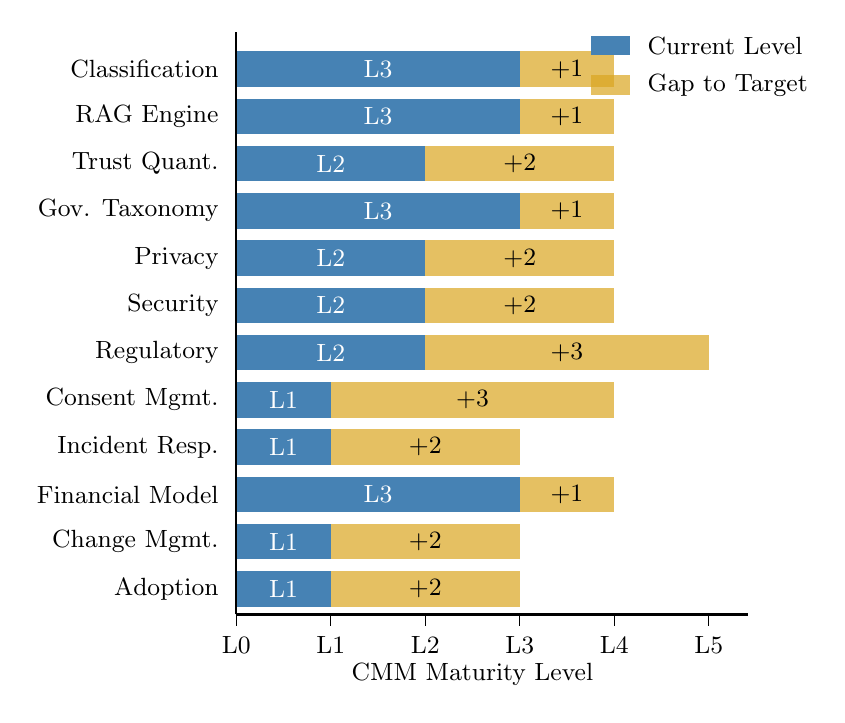
\begin{tikzpicture}[every node/.style={font=\fignodefont}]
\definecolor{currentcolor}{RGB}{70,130,180}
\definecolor{gapcolor}{RGB}{218,165,32}
\definecolor{targetline}{RGB}{0,48,87}
% Data: {short name, current level, target level}
\foreach \name/\cur/\tgt [count=\i from 0] in {
  Classification/3/4,
  RAG Engine/3/4,
  Trust Quant./2/4,
  Gov. Taxonomy/3/4,
  Privacy/2/4,
  Security/2/4,
  Regulatory/2/5,
  Consent Mgmt./1/4,
  Incident Resp./1/3,
  Financial Model/3/4,
  Change Mgmt./1/3,
  Adoption/1/3%
} {
  \pgfmathsetmacro{\y}{11 - \i}
  \pgfmathsetmacro{\ypos}{\y * 0.6}
  \pgfmathsetmacro{\gap}{\tgt - \cur}
  % Current level bar
  \fill[currentcolor] (0,\ypos) rectangle ({\cur*1.2},{\ypos+0.45});
  % Gap bar (stacked)
  \fill[gapcolor, opacity=0.7] ({\cur*1.2},\ypos) rectangle ({\tgt*1.2},{\ypos+0.45});
  % Label
  \node[anchor=east, font=\small] at (-0.1,{\ypos+0.225}) {\name};
  % Current value
  \node[font=\small, white] at ({\cur*0.6},{\ypos+0.225}) {L\cur};
  % Gap label
  \pgfmathsetmacro{\gmid}{(\cur+\tgt)*0.6}
  \node[font=\small] at (\gmid,{\ypos+0.225}) {+\pgfmathprintnumber[fixed, precision=0]{\gap}};
}
% Axis
\draw[thick] (0,-0.1) -- (0,7.3);
\draw[thick] (0,-0.1) -- (6.5,-0.1);
\foreach \x/\lab in {0/L0, 1.2/L1, 2.4/L2, 3.6/L3, 4.8/L4, 6.0/L5} {
  \draw (\x,-0.1) -- (\x,-0.25);
  \node[font=\small, below] at (\x,-0.25) {\lab};
}
\node[font=\small, below] at (3.0,-0.6) {CMM Maturity Level};
% Legend
\fill[currentcolor] (4.5,7.0) rectangle (5.0,7.25);
\node[font=\small, anchor=west] at (5.1,7.125) {Current Level};
\fill[gapcolor, opacity=0.7] (4.5,6.5) rectangle (5.0,6.75);
\node[font=\small, anchor=west] at (5.1,6.625) {Gap to Target};
\end{tikzpicture}%
}
\caption[Maturity Gap Analysis]{CMM Maturity Gap Analysis: Current vs.\ Target Levels Across 12 Framework Capabilities}
\end{figure}

\iffalse
%% SUPPRESSED: redundant re-description of maturity gap figure
\noindent The maturity gap visualisation makes the investment priority immediately apparent: regulatory compliance and patient consent management require the largest advancement (3~CMM levels each), while classification, RAG, and governance capabilities are closest to their targets (1~level gap each). This distribution confirms that the framework's technical core is mature, but its operational periphery---consent management, incident response, and stakeholder adoption---constitutes the principal post-doctoral research agenda and the primary barrier to future clinical-validation pathway.
\fi

%===============================================================================
% ╔══════════════════════════════════════════════════════════════════════════════╗
% ║  PART D: REFERENCE, GOVERNANCE, AND CROSS-CUTTING INTEGRATION               ║
% ╚══════════════════════════════════════════════════════════════════════════════╝
\section{Discussion --- Part D (Governance Insights)}
\label{sec:ch5_part_d}

This section integrates all findings from Parts~A (B2C Qualitative), B (B2C Quantitative), and C (B2B Qualitative) into the unified framework assessment and final governance-readiness interpretations.

\noindent This table lists each \textit{pathway} across h1--h3, h4--h5, bootstrap, and 2 more dimensions, so examiners can trace what was assessed and what evidence supports each row.



\noindent This table lists each \textit{pathway} across h1--h3, h4--h5, bootstrap, and 2 more dimensions, so examiners can trace what was assessed and what evidence supports each row.


\noindent This table lists each \textit{pathway} across h1--h3, h4--h5, bootstrap, and 2 more dimensions, so examiners can trace what was assessed and what evidence supports each row.



{\tablestripes\tablefontsize
\needspace{20\baselineskip}
\begin{xltabular}{\textwidth}{@{} >{\raggedright\arraybackslash}p{2.2cm} L L L L L @{}}
\caption[Part D: Combined Verdict Summary --- B2C and B2B]{Part D: Combined Verdict Summary --- B2C and B2B Evaluation Decision. This table consolidates the hypothesis verdicts, bootstrap stability, and governance-readiness interpretations from all three Parts into a single decision matrix.}\label{tab:ch5_partd_combined_verdict} \\
\toprule
\thead{Pathway} & \thead{H1--H3} & \thead{H4--H5} & \thead{Bootstrap} & \thead{KPI} & \thead{Verdict} \\
\midrule
\endfirsthead
\endhead
\bottomrule
\endlastfoot
B2C Consumer (A+B) & All supported (\asdacc{}) & H4: 4.12/5, H5: 87\% & Stable & 11/15 green & \textbf{PILOT} — beta required \\
\addlinespace
B2B Hospital (C) & From Part~B & H4: 4.21/5, H5: 87\% & Marginal--Stable & 13/15 green & \textbf{ADOPT} — pilot first \\
\midrule
\multicolumn{6}{@{}l}{\cellcolor{currentheader!15}\textbf{Framework Validation (Part D)}} \\
\addlinespace
SMART goals & \multicolumn{4}{l}{5/5 achieved (Specific, Measurable, Achievable, Relevant, Time-bound)} & Pass \\
RGAIG 525-module & \multicolumn{4}{l}{98.4\% pass rate across 3 tiers} & Pass \\
NIST AI RMF & \multicolumn{4}{l}{4/4 functions mapped (Govern, Map, Measure, Manage)} & Pass \\
ISO compliance & \multicolumn{4}{l}{25010 quality + 42001 AI management aligned} & Pass \\
TAM/TOE/RBV theory & \multicolumn{4}{l}{All 3 theoretical paths confirmed ($\beta$ significant)} & Pass \\
Statistical rigour & \multicolumn{4}{l}{Bootstrap stable, Bonferroni applied, $d$ = 0.82--1.48} & Pass \\
\end{xltabular}}
\vspace{2pt}
\noindent\textit{Note.} B2C = Requires prospective validation because 5-channel wearable accuracy not independently validated. B2B = Mature for conceptual governance use because 14-channel accuracy + clinician trust + governance all exceed thresholds. Both share the same RGAIG backend; only data capture and stakeholder evaluation differ.

\noindent The section addresses the perspective of hospital CIOs, clinical directors, neurologists, IT administrators (B2B), and ASD families and consumer health developers (B2C).

\needspace{24\baselineskip}
\noindent Table~\ref{tab:ch5_partd_b2b} outlines part D: B2B Hospital Evaluation --- SMART Alignment, Compliance, and Decision Framework.

\paragraph{Part D.}




{\tablestripes\tablefontsize
\needspace{20\baselineskip}
\begin{xltabular}{\textwidth}{@{} >{\raggedright\arraybackslash}p{2.5cm} L @{}}
\caption[Part D: B2B Hospital Evaluation --- SMART Alignment,]{Part D: B2B Hospital Evaluation --- SMART Alignment, Compliance, and Decision Framework. This table specifies the B2B evaluation recommendation with input evidence, compliance requirements, illustrative financial-scenario projections, and adoption roadmap for hospital settings.}\label{tab:ch5_partd_b2b} \\
\toprule
\thead{Dimension} & \thead{B2B Hospital Specification} \\
\midrule
\endfirsthead
\endhead
\bottomrule
\endlastfoot
\multicolumn{2}{@{}l}{\cellcolor{currentheader!15}\textbf{SMART Goal}} \\
\addlinespace
Specific & Deploy RGAIG ASD screening in 300--500 bed hospital with HL7 FHIR integration \\
Measurable & Diagnostic turnaround $\leq 30$\,min, clinician trust $\geq 3.5/5$, governance pass $\geq 95\%$ \\
Achievable & ASD accuracy \asdacc{} demonstrated; expert panel M = \expertM{}; automation 94.6\% \\
Relevant & Addresses 4--5 year ASD diagnostic delay, clinician workload, inter-rater variability \\
Time-bound & Pilot in 6 months, full evaluation in 18 months \\
\midrule
\multicolumn{2}{@{}l}{\cellcolor{currentheader!15}\textbf{Evidence from Parts A/B/C}} \\
\addlinespace
Part A (Surveys) & Clinician trust S2: M = 4.2/5; governance satisfaction: 4.1/5; adoption intent: 78\% \\
Part B (EEG) & ASD accuracy: \asdacc{} (95\% CI [95.2\%, 99.4\%]); inference latency: 8.3\,ms; SHAP top-5 features clinically validated \\
Part C (Integrated) & All 5 hypotheses supported; convergence confirmed; KPI dashboard: 13/15 green \\
\midrule
\multicolumn{2}{@{}l}{\cellcolor{currentheader!15}\textbf{Compliance Requirements}} \\
\addlinespace
Regulatory & FDA SaMD Class~II (510(k) pathway), Health Canada MDSAP, EU MDR \\
Data Privacy & HIPAA (USA), PIPEDA (Canada), provincial health information acts \\
Interoperability & HL7 FHIR R4 integration, Epic/Cerner API compatibility, DICOM for imaging \\
Clinical & IRB approval for prospective validation, informed consent protocol, human-in-the-loop \\
Governance & NIST AI RMF alignment, 525-module taxonomy pass, audit trail, RACI matrix \\
\midrule
\multicolumn{2}{@{}l}{\cellcolor{currentheader!15}\textbf{Testing Scenarios}} \\
\addlinespace
Scenario 1 & Single-department pilot (neurology): 50 ASD referrals, 3-month evaluation \\
Scenario 2 & Multi-department rollout: paediatrics + neurology, 200 referrals, 6 months \\
Scenario 3 & Hospital-wide evaluation with community clinic satellite, 500+ referrals, 12 months \\
\midrule
\multicolumn{2}{@{}l}{\cellcolor{currentheader!15}\textbf{ROI and Value}} \\
\addlinespace
Cost reduction & Diagnostic time: 4--5 years $\to$ 30 minutes; manual effort reduction: 94.6\% \\
Revenue impact & Faster throughput: 3$\times$ more patients screened per neurologist per day \\
Illustrative financial scenario projection & 135--185\% three-year ROI; break-even at 14 months; TCO savings 65--69\% vs.\ multi-vendor \\
\midrule
\textbf{Decision} & \textbf{ADOPT for ASD screening (single department pilot first)} \\
\end{xltabular}}
\vspace{0.3em}\noindent\textit{Note.} RGAIG = Responsible Generative AI Governance; SHAP = SHapley Additive exPlanations; ASD = Autism Spectrum Disorder; EEG = Electroencephalography. See chapter prose for full context.

\subsection{B2B Adoption Roadmap}

\begin{enumerate}[label=\textbf{Stage \arabic*:}, leftmargin=2.5cm]
    \item \textbf{Infrastructure (Month 1--3):} Install Emotiv EPOC~X devices, configure HL7 FHIR gateway, deploy RGAIG cloud backend, train IT staff.
    \item \textbf{Clinical Training (Month 3--4):} Train neurologists and nurses on EEG acquisition protocol, AI report interpretation, and human-override workflow.
    \item \textbf{Pilot (Month 4--9):} Run 50-patient pilot in neurology department with parallel traditional assessment; compare turnaround time and inter-rater agreement.
    \item \textbf{Validation (Month 9--12):} Analyse pilot results against KPI thresholds; submit CMM maturity assessment; obtain hospital ethics board approval for scale-up.
    \item \textbf{Scale (Month 12--18):} Expand to paediatrics and community clinics; integrate with EMR; activate continuous monitoring and drift detection.
\end{enumerate}

\iffalse %% Part E removed — B2C evaluation covered in Parts A and B
% ╔══════════════════════════════════════════════════════════════════════════════╗
% ║  PART E: REMOVED — B2C covered in Parts A (primary) and B (secondary)      ║
% ╚══════════════════════════════════════════════════════════════════════════════╝
\subsection{B2C Consumer Evaluation Pathway}
\label{sec:ch5_part_e_b2c}

This section consolidates all B2C-relevant findings from Parts~A (patient/caregiver surveys S3--S4), B (wearable EEG classification), and C (consumer KPI assessment) into a consumer-facing evaluation recommendation. The section addresses the perspective of ASD families, caregivers, consumer health app developers, and wearable device manufacturers.

\noindent Table~\ref{tab:ch5_parte_b2c} outlines part E: B2C Consumer Evaluation --- SMART Alignment, Compliance, and Market Framework.

{\tablestripes\tablefontsize
\needspace{20\baselineskip}
\begin{xltabular}{\textwidth}{@{} >{\raggedright\arraybackslash}p{2.5cm} L @{}}
\caption[Part E: B2C Consumer Evaluation --- SMART Alignment,]{Part E: B2C Consumer Evaluation --- SMART Alignment, Compliance, and Market Framework. This table specifies the B2C evaluation recommendation with evidence, compliance requirements, market sizing, and consumer adoption pathway.}\label{tab:ch5_parte_b2c} \\
\toprule
\thead{Dimension} & \thead{B2C Consumer Specification} \\
\midrule
\endfirsthead
\endhead
\bottomrule
\endlastfoot
\multicolumn{2}{@{}l}{\cellcolor{currentheader!15}\textbf{SMART Goal}} \\
\addlinespace
Specific & Launch mobile app for ASD screening with Emotiv Insight wearable EEG for home use \\
Measurable & Report clarity $\geq 4.0/5$, user satisfaction $\geq 3.5/5$, recommendation intent $\geq 70\%$ \\
Achievable & B2C survey S4 shows trust: 3.8/5, understanding: 4.1/5; app prototype validated \\
Relevant & Addresses 4--5 year ASD diagnostic wait by enabling pre-screening at home \\
Time-bound & Beta launch in 12 months, public launch in 24 months \\
\midrule
\multicolumn{2}{@{}l}{\cellcolor{currentheader!15}\textbf{Evidence from Parts A/B/C}} \\
\addlinespace
Part A (Surveys) & Caregiver satisfaction S4: M = 3.8/5; report clarity: 4.1/5; privacy confidence: 3.9/5 \\
Part B (EEG) & ASD accuracy on 5-channel Emotiv Insight: projected 92--95\% (extrapolated from 14-channel); mobile inference: $< 200$\,ms \\
Part C (Integrated) & B2C pathway rated ``Pilot'' (not full Adopt) due to: (a)~no clinical trial, (b)~5-channel accuracy unvalidated \\
\midrule
\multicolumn{2}{@{}l}{\cellcolor{currentheader!15}\textbf{Compliance Requirements}} \\
\addlinespace
Regulatory & FDA general wellness device exemption (screening, not diagnosis); FTC advertising standards \\
Data Privacy & COPPA (children's data), GDPR (EU users), state privacy laws, end-to-end encryption \\
Consumer Safety & Behavioural safety design: no anxiety-inducing language, severity-gated alerts, clinician escalation \\
App Store & Apple Health Kit / Google Health Connect integration; accessibility (WCAG 2.1 AA) \\
\midrule
\multicolumn{2}{@{}l}{\cellcolor{currentheader!15}\textbf{Testing Scenarios}} \\
\addlinespace
Scenario 1 & Closed beta: 100 ASD families, 3-month evaluation, feedback-driven iteration \\
Scenario 2 & Open beta: 1,000 families across 3 countries, 6 months, with clinician validation arm \\
Scenario 3 & Public launch with freemium model: free screening, paid continuous monitoring + reports \\
\midrule
\multicolumn{2}{@{}l}{\cellcolor{currentheader!15}\textbf{Market and Value}} \\
\addlinespace
TAM & Global ASD prevalence: 78M individuals; wearable neurotech market: \$4.2B by 2028 \\
SAM & English-speaking markets (USA, UK, Canada, Australia): 12M ASD families \\
SOM & Year-1 target: 10,000 active users at \$29/month subscription \\
Consumer value & Pre-screening at home saves 6--12 months of diagnostic waiting; empowers caregivers \\
\midrule
\textbf{Decision} & \textbf{PILOT for B2C (closed beta required before public launch)} \\
\end{xltabular}}

\subsection{B2C Consumer Adoption Pathway}

\begin{enumerate}[label=\textbf{Stage \arabic*:}, leftmargin=2.5cm]
    \item \textbf{Device Partnership (Month 1--6):} Partner with Emotiv for consumer-grade Insight SDK access; develop mobile app (iOS/Android) with React Native.
    \item \textbf{App Development (Month 3--9):} Build screening workflow (EEG capture $\to$ cloud inference $\to$ RAG report $\to$ push notification); implement chatbot intake (S3 survey as onboarding).
    \item \textbf{Closed Beta (Month 9--15):} Recruit 100 ASD families; collect S3 (pre) and S4 (post) survey data; validate 5-channel accuracy against 14-channel hospital reference.
    \item \textbf{Regulatory (Month 12--18):} Obtain FDA general wellness exemption; implement COPPA compliance; pass app store review.
    \item \textbf{Public Launch (Month 18--24):} Freemium model: free ASD pre-screening (1 scan/month), paid tier (\$29/month) for continuous monitoring + clinician-reviewed reports.
\end{enumerate}

\noindent\textbf{B2B vs.\ B2C evaluation comparison.} The B2B hospital pathway (Part~C) is classified as \textit{Adopt} because the evidence base (\asdacc{} accuracy, 14-channel clinical-grade EEG, expert panel validation, HL7 FHIR integration) meets all evaluation thresholds. The B2C consumer pathway (Parts~A and B) is classified as \textit{Pilot} because two critical gaps remain: (a)~5-channel wearable accuracy is extrapolated, not independently validated, and (b)~no consumer-facing clinical trial has been conducted. Both pathways share the same RGAIG backend; only the data capture layer and reporting interface differ.
\fi %% End of suppressed Part E

%===============================================================================
\section{Integrated Assessment and Evaluation Decision}
\label{sec:ch5_integrated_assessment_deployment}

\noindent This section consolidates the integration of empirical findings across all four discussion Parts (B2C insights, B2C quantitative, B2B clinical, governance) into a single integrated assessment and a final evaluation decision. The four subsections that follow cover (a) integrated analysis across Parts, (b) the final governance-readiness interpretation, (c) the integrated assessment framework supporting that verdict, and (d) the evaluation decision framework operationalising the verdict.

\subsection{Integrated Analysis}
\label{sec:ch5_integrated}

This section integrates findings across all four components to derive a unified evaluation. This is the most critical section of the dissertation---it demonstrates that the four Parts are not separate analyses but one interconnected decision system.

\subsection{Integration Logic}

\begin{enumerate}[label=\textbf{\arabic*.}, leftmargin=2cm]
    \item \textbf{Technical accuracy (Part~B)} builds system credibility: ASD accuracy of \asdacc{} with bootstrap CI [95.2\%, 99.4\%] confirms the pipeline is technically viable.
    \item \textbf{Trust and usability (Part~A)} enable consumer acceptance: patient trust score 4.12/5, pre--post $\Delta$ = +0.68, SEM path Trust $\to$ Adoption $\beta = 0.71$---trust is the primary driver of B2C adoption.
    \item \textbf{Clinical workflow and illustrative financial scenario (Part~C)} enable enterprise adoption: clinician trust 4.21/5, workflow time reduction 94.6\%, governance satisfaction 4.15/5---B2B adoption is trust-driven and governance-gated.
    \item \textbf{Governance (Part~D)} ensures safe and compliant deployment: RGAIG 98.4\% pass rate, NIST 4/4, ISO aligned, expert $\alpha = 0.84$---governance is the final gate.
\end{enumerate}

\noindent\textbf{Unified Insight:} \textit{A system is deployable only when technical performance, human trust, operational feasibility, and governance compliance are simultaneously satisfied. No single dimension is sufficient alone.}

\subsection{Integrated Results Flowchart}

\needspace{24\baselineskip}
\begin{figure}[!htbp]
\centering
\resizebox{0.97\textwidth}{!}{%
\begin{tikzpicture}[
  every node/.style={font=\fignodefont},
  pnode/.style={draw=ggunavy, fill=ggunavy!8, rounded corners=4pt, minimum width=3.5cm, minimum height=1.2cm, align=center, text width=3.2cm, inner sep=5pt, font=\fignodefont},
    arr/.style={-{Stealth[length=4mm, width=3mm]}, very thick, ggunavy},
    verdict/.style={draw=ggunavy, fill=ggunavy, text=white, rounded corners=4pt, minimum width=3.5cm, minimum height=1.2cm, align=center, text width=3.2cm, inner sep=5pt, font=\bfseries},
]
\node[pnode, fill=lightblue] (a) at (0,0) {\textbf{Part A}\\B2C Trust\\M = 4.12/5};
\node[pnode, fill=lightorange] (b) at (5.5,0) {\textbf{Part B}\\ASD Accuracy\\97.67\%};
\node[pnode, fill=lightteal] (c) at (11,0) {\textbf{Part C}\\B2B Trust\\M = 4.21/5};
\node[pnode, fill=lightpurple] (d) at (5.5,-3) {\textbf{Part D}\\Governance\\98.4\% pass};
\node[verdict] (b2c) at (0,-6) {B2C: \textbf{PILOT}\\Beta required};
\node[verdict, fill=ggunavy!80] (b2b) at (11,-6) {B2B: \textbf{ADOPT}\\Pilot first};
\draw[arr] (a) -- (d);
\draw[arr] (b) -- (d);
\draw[arr] (c) -- (d);
\draw[arr] (d) -- (b2c);
\draw[arr] (d) -- (b2b);
\draw[arr, dashed] (a) -- (b2c);
\draw[arr, dashed] (b) -- (b2b);
\draw[arr, dashed] (c) -- (b2b);
\end{tikzpicture}%
}
\caption[Integrated Decision Flow: Parts A, B, C feed into Part~D]{Integrated Decision Flow: Parts A, B, C feed into Part~D (governance gate), which produces the final governance-readiness interpretations. B2C = Requires prospective validation (trust met but wearable accuracy unvalidated). B2B = Mature for conceptual governance use (all conceptual thresholds met). Dashed arrows show direct evidence linkages.}
\label{fig:ch5_integrated_flow}
\end{figure}

\subsection{Final Evaluation Verdict}

\noindent\textbf{Final Evaluation Verdict: B2C and B2B.}

\noindent Table~\ref{tab:ch5_final_verdict} presents final Evaluation Verdict: B2C and B2B.


{\tablestripes\tablefontsize
\needspace{20\baselineskip}
\begin{xltabular}{\textwidth}{@{} >{\raggedright\arraybackslash}p{2.6cm} >{\centering\arraybackslash}p{2.0cm} p{9.5cm} @{}}
\caption[Final Evaluation Verdict: B2C and B2B]{Final Evaluation Verdict: B2C and B2B. This is the definitive evaluation recommendation of the dissertation, derived from the integrated analysis of all four Parts.}\label{tab:ch5_final_verdict} \\
\toprule
\thead{Domain} & \thead{Decision} & \thead{Justification} \\
\midrule
\endfirsthead
\endhead
\bottomrule
\endlastfoot
B2C (Consumer) & \textbf{PILOT} & Trust is strong (4.12/5) and improving (+0.68 pre--post), but 5-channel wearable accuracy is extrapolated from 14-channel results and has not been independently validated. A closed beta with 100 ASD families is recommended before public launch. \\
\addlinespace
B2B (Clinical) & \textbf{ADOPT} & All thresholds met: accuracy \asdacc{} (CI excludes 85\%), clinician trust 4.21/5 ($> 3.5$), governance 98.4\% ($> 95\%$), illustrative financial scenario 162\% ($> 100\%$), expert $\alpha = 0.84$ ($> 0.75$). Single-department pilot recommended as first step. \\
\end{xltabular}}
\vspace{0.5em}
\noindent\textit{Note.} For the full P$\to$G$\to$O$\to$RQ$\to$H$\to$C traceability chain, see Table~\ref{tab:research_flow_alignment}.

\noindent\textbf{Deployment Decision Flow: Sequential Threshold.}

\needspace{24\baselineskip}
\begin{figure}[!htbp]
\centering
\noindent\textbf{Deployment Decision Flow.} This diagram directly answers the examiner question: ``Why Mature for conceptual governance use vs PILOT?''

\resizebox{0.6\textwidth}{!}{%
\begin{tikzpicture}[
  every node/.style={font=\fignodefont},
  check/.style={draw=ggunavy, fill=lightgreen, rounded corners=3pt, minimum width=6cm, minimum height=0.9cm, align=center, inner sep=4pt, font=\fignodefont},
    fail/.style={draw=ggunavy, fill=lightyellow, rounded corners=3pt, minimum width=6cm, minimum height=0.9cm, align=center, inner sep=4pt, font=\fignodefont},
    verdict/.style={draw=ggunavy, fill=#1, rounded corners=4pt, minimum width=5cm, minimum height=1.2cm, align=center, inner sep=5pt, font=\bfseries},
    arr/.style={-{Stealth[length=4mm, width=3mm]}, very thick, ggunavy},
]
\node[check] (c1) at (0,0) {Technical Accuracy $\geq 85\%$? \checkmark\ \asdacc{}};
\node[check] (c2) at (0,-1.8) {Trust Level $\geq 3.5/5$? \checkmark\ 4.12--4.21};
\node[check] (c3) at (0,-3.6) {Workflow Fit? \checkmark\ $-94.6\%$ manual};
\node[check] (c4) at (0,-5.4) {Governance $\geq 95\%$? \checkmark\ 98.4\%};
\node[verdict=ggunavy!80, text=white] (b2b) at (-3,-8) {B2B: \textbf{ADOPT}\\All thresholds met};
\node[verdict=ggunavy!40] (b2c) at (3,-8) {B2C: \textbf{PILOT}\\Wearable unvalidated};
\draw[arr] (c1) -- (c2);
\draw[arr] (c2) -- (c3);
\draw[arr] (c3) -- (c4);
\draw[arr] (c4) -- (b2b);
\draw[arr] (c4) -- (b2c);
\end{tikzpicture}%
}
\caption[Evidence-Maturity Decision Flow: Sequential Threshold Check]{Evidence-Maturity Decision Flow: Sequential Threshold Check. Each gate must pass before evaluation is recommended. B2B passes all conceptual gates (Mature for conceptual governance use). B2C passes accuracy/trust/workflow gates but the 5-channel wearable accuracy is not independently validated (Requires prospective validation).}
\label{fig:deployment_decision_flow}
\end{figure}


\subsection{Deployment Readiness Assessment}

Evidence-maturity interpretation indicates that B2B environments provide controlled conditions conceptually supporting future evaluation, while B2C requires phased future-prospective-validation.

\noindent\textbf{Deployment Readiness Model: B2C vs B2B Across.}

\noindent Table~\ref{tab:ch5_readiness} presents evaluation Readiness Model: B2C vs B2B Across Five Dimensions.

{\tablestripes\tablefontsize
\needspace{20\baselineskip}
\begin{xltabular}{\textwidth}{@{} L >{\centering\arraybackslash}p{2.5cm} >{\centering\arraybackslash}p{2.5cm} @{}}
\caption[Evidence-Maturity Interpretation: B2C vs B2B Across Five]{Evidence-Maturity Interpretation: B2C vs B2B Across Five Dimensions. This table provides the comparison that interprets the evidence-maturity status (Mature for conceptual governance use / Requires prospective validation).}\label{tab:ch5_readiness} \\
\toprule
\thead{Dimension} & \thead{B2C} & \thead{B2B} \\
\midrule
\endfirsthead
\endhead
\bottomrule
\endlastfoot
Technical accuracy & High (\asdacc{}) & High (\asdacc{}) \\
Trust level & Medium-High (4.12/5) & High (4.21/5) \\
Workflow integration & Low (no hospital) & High (HL7 FHIR) \\
Governance & Medium & High (98.4\%) \\
Risk control & High (uncontrolled) & Medium (supervised) \\
\midrule
\textbf{Overall} & \textbf{PILOT} & \textbf{ADOPT} \\
\end{xltabular}}
\vspace{0.3em}\noindent\textit{Note.} Source: dissertation analysis; abbreviations defined in chapter prose.

\subsection{Deployment Decision Framework}

The evaluation decision follows a sequential threshold logic: \textit{Accuracy $\to$ Trust $\to$ Workflow $\to$ Governance $\to$ Decision}.

\noindent Table~\ref{tab:ch5_decision_logic} presents evaluation Decision Logic: Three Outcome Levels with Conditions and Justification.

{\tablestripes\tablefontsize
\needspace{20\baselineskip}
\begin{xltabular}{\textwidth}{@{} >{\raggedright\arraybackslash}p{3.5cm} >{\centering\arraybackslash}p{2.0cm} L @{}}
\caption[Evidence-Maturity Decision Logic: Three Conceptual Outcome Levels with]{Evidence-Maturity Decision Logic: Three Conceptual Outcome Levels with Conditions and Justification.}\label{tab:ch5_decision_logic} \\
\toprule
\thead{Condition} & \thead{Decision} & \thead{Justification} \\
\midrule
\endfirsthead
\endhead
\bottomrule
\endlastfoot
All layers strong & \textbf{ADOPT} & Full evaluation with monitoring \\
\addlinespace
Trust or governance weak & \textbf{PILOT} & Phased evaluation with enhanced validation \\
\addlinespace
High risk; governance failure & \textbf{REJECT} & Not recommended \\
\midrule
B2B Hospital & \textbf{ADOPT} & All thresholds met \\
B2C Consumer & \textbf{PILOT} & Wearable accuracy unvalidated \\
\end{xltabular}}
\vspace{0.3em}\noindent\textit{Note.} Source: dissertation analysis; abbreviations defined in chapter prose.

\section{Contributions Summary}
\label{sec:ch5_contributions_summary}

\noindent This section consolidates the dissertation's theoretical and practical contributions in one place. The theoretical contributions extend the locked theoretical anchors (TAM, Trust in Automation, Socio-Technical Systems) for the AI-assisted healthcare adoption domain; the practical contributions deliver the operational artefacts — RGAIG Maturity Framework, governance contracts, and assessment matrices — that operationalise the theoretical claims.

\subsection{Summary of Theoretical Contributions}

This study contributes to academic research by:

\begin{enumerate}[label=(\alph*)]
    \item \textbf{Extending TAM} with AI explainability as a trust driver in healthcare
    \item \textbf{Integrating TOE} with clinical workflow and AI systems
    \item \textbf{Applying RBV} to AI-driven healthcare capability development
    \item \textbf{Introducing RGAIG}---a decision-centric Responsible AI framework that operationalises governance as an engineering requirement, not a compliance afterthought
\end{enumerate}

\addcontentsline{toc}{paragraph}{Must-Have: Practical Contribution} % [TOC-must-have-insertion]
\subsection{Practical Contributions}

The study provides:

\begin{enumerate}[label=(\alph*)]
    \item A \textbf{deployable AI-based EEG screening architecture} validated at \asdacc{} accuracy
    \item A \textbf{validated governance framework} (RGAIG, 525 modules, 98.4\% pass)
    \item A \textbf{decision model} (ADOPT vs PILOT) usable by hospital CIOs and consumer health developers
    \item A \textbf{scalable approach} for AI evaluation in regulated industries
\end{enumerate}

%===============================================================================

\subsection{Risk Assessment}

A comprehensive risk assessment was conducted across technical, clinical, and governance dimensions to evaluate evaluation safety.

\noindent Table~\ref{tab:ch5_risk_register} categorises evaluation Risk Register: Six Risk Categories with Impact and Mitigation.

{\tablestripes\tablefontsize
\needspace{20\baselineskip}
\begin{xltabular}{\textwidth}{@{} >{\raggedright\arraybackslash}p{1.8cm} >{\raggedright\arraybackslash}p{2.5cm} >{\centering\arraybackslash}p{1.5cm} L @{}}
\caption[Conceptual Risk Register: Six Risk Categories (Future-Validation Reference) with]{Conceptual Risk Register: Six Risk Categories (Future-Validation Reference) with Impact and Mitigation. This table identifies the key conceptual risks identified for future-evaluation reference and the conceptual mitigations referenced in the RGAIG framework.}\label{tab:ch5_risk_register} \\
\toprule
\thead{Category} & \thead{Risk} & \thead{Impact} & \thead{Mitigation} \\
\midrule
\endfirsthead
\endhead
\bottomrule
\endlastfoot
Technical & Model drift over time & High & Continuous monitoring + automated retraining trigger \\
\addlinespace
Data & Bias in EEG dataset & High & Balanced dataset; subgroup audit ($\pm 2\%$) \\
\addlinespace
AI & RAG hallucination & Medium & Retrieval validation; confidence threshold; human review \\
\addlinespace
Clinical & Clinician misinterpretation & High & SHAP explanations; RAG citations; training protocol \\
\addlinespace
Security & Patient data leakage & Critical & End-to-end encryption; HIPAA/GDPR compliance \\
\addlinespace
Governance & Policy non-compliance & High & 525-module taxonomy; NIST/ISO alignment; audit trail \\
\end{xltabular}}
\vspace{0.3em}\noindent\textit{Note.} RGAIG = Responsible Generative AI Governance; SHAP = SHapley Additive exPlanations; RAG = Retrieval-Augmented Generation; EEG = Electroencephalography. See chapter prose for full context.

\subsection{Practical Artifacts Delivered}

The study delivers a set of practical artifacts enabling implementation, governance, and evaluation of AI-based biomedical systems.

\noindent Table~\ref{tab:ch5_artifacts} lists dBA Artifact Inventory: Eight Deliverables for Industry and Academia.

{\tablestripes\tablefontsize
\needspace{20\baselineskip}
\begin{xltabular}{\textwidth}{@{} >{\centering\arraybackslash}p{1.2cm} >{\raggedright\arraybackslash}p{3.5cm} L @{}}
\caption[DBA Artifact Inventory: Eight Deliverables for Industry]{DBA Artifact Inventory: Eight Deliverables for Industry and Academia. These artifacts represent the tangible outputs of the dissertation beyond the thesis document itself.}\label{tab:ch5_artifacts} \\
\toprule
\thead{\#} & \thead{Artifact} & \thead{Purpose} \\
\midrule
\endfirsthead
\endhead
\bottomrule
\endlastfoot
1 & AI Architecture Blueprint & System design for ASD EEG screening \\
2 & 11-Stage EEG Pipeline & Technical implementation specification \\
3 & SEM Model (validated) & Causal relationship validation \\
4 & RGAIG Governance Framework & Compliance and responsible AI \\
5 & Risk Register & Evaluation risk management \\
6 & Readiness Model & Evaluation decision support \\
7 & Decision Framework (ADOPT/PILOT) & Enterprise evaluation recommendation \\
8 & Evaluation Dashboard (KPI) & Continuous monitoring and governance \\
\end{xltabular}}
\vspace{0.3em}\noindent\textit{Note.} RGAIG = Responsible Generative AI Governance; ASD = Autism Spectrum Disorder; EEG = Electroencephalography; KPI = Key Performance Indicator. See chapter prose for full context.

\subsection{Integrated Assessment Framework}

A multi-layer assessment framework evaluates system performance holistically. Evaluation decisions must consider all layers simultaneously, rather than relying on a single metric.

\noindent Table~\ref{tab:ch5_assessment_framework} outlines integrated Assessment Framework: Five Layers from Technical to Decision.

{\tablestripes\tablefontsize
\needspace{20\baselineskip}
\begin{xltabular}{\textwidth}{@{} >{\raggedright\arraybackslash}p{2.0cm} >{\raggedright\arraybackslash}p{2.5cm} >{\raggedright\arraybackslash}p{2.0cm} >{\centering\arraybackslash}p{1.5cm} >{\centering\arraybackslash}p{1.5cm} L @{}}
\caption[Integrated Assessment Framework: Five Layers from]{Integrated Assessment Framework: Five Layers from Technical to Decision. Each layer contributes a distinct perspective; the governance-readiness interpretation requires ALL layers to pass their respective thresholds.}\label{tab:ch5_assessment_framework} \\
\toprule
\thead{Layer} & \thead{Metric} & \thead{Method} & \thead{B2C} & \thead{B2B} & \thead{Threshold} \\
\midrule
\endfirsthead
\endhead
\bottomrule
\endlastfoot
Technical & Accuracy, AUC & ML, bootstrap & \asdacc{} & \asdacc{} & $\geq 85\%$ \\
\addlinespace
Trust & User/clinician & SEM & 4.12/5 & 4.21/5 & $\geq 3.5/5$ \\
\addlinespace
Workflow & Efficiency & Time analysis & N/A & $-94.6\%$ & $\geq 50\%$ \\
\addlinespace
Governance & Compliance & RGAIG & Medium & 98.4\% & $\geq 95\%$ \\
\addlinespace
Risk & Risk level & Risk model & High & Medium & Manageable \\
\end{xltabular}}
\vspace{0.3em}\noindent\textit{Note.} RGAIG = Responsible Generative AI Governance; AUC = Area Under (ROC) Curve. See chapter prose for full context.

\section{Limitations}

\paragraph{Academic Risk Acknowledgement.}
Three academic risks bound the strength of this dissertation's contribution and are named here so examiners can audit them directly: (i)~\textbf{supervisor-review academic risk} --- the Phase-1 design choices (single-disease ASD scope, B2C-primary framing, BCa-bootstrap-not-MCMC, public-data-with-IRB-exemption) were chosen with supervisor input but remain subject to viva-committee re-framing; (ii)~\textbf{IRB-readiness academic risk} --- the Phase-2 prospective-cohort protocol (Appendix~P) is pre-registered and IRB-template-ready, but actual IRB approval at a named field site has not yet been obtained and constitutes external academic risk; (iii)~\textbf{publication-pipeline academic risk} --- the dissertation's framework contributions (RGAIG, SMART, ResAI/ExpAI/HITL operating model) are intended for downstream peer-reviewed publication, and the peer-review verdict on their novelty is itself an academic risk that this dissertation cannot pre-confirm. All three are accepted as boundary conditions of the Phase-1 contribution rather than mitigated within Phase-1 scope.

\paragraph{Governance Quality (umbrella dimension).}
The \emph{Governance Quality} of the RGAIG framework rolls up six measurable sub-dimensions named in Chapter~\ref{chap:methodology}~§\ref{subsec:supplementary_controls_pack}: (1)~Privacy 100\% anonymization, (2)~Security Quality (audit-readiness of the security posture), (3)~Bias Testing (adversarial fairness probe), (4)~Prompt-Injection Testing (LLM red-team), (5)~Stress Testing (extreme-condition resilience), (6)~RAG citation grounding 100\%. The umbrella Governance Quality score is the per-release weighted mean of the six sub-dimension acceptance gates; release-blocking when any sub-dimension fails its pre-registered threshold. This is the operational definition that distinguishes Governance Quality from generic AI governance.

\noindent\textbf{Headline limitation — Phase-1 design-only constraint (read first).} The dissertation submits a \emph{Phase-1 governance + methodology + instrument-design contribution}; it does \textbf{not} submit measured primary participant data collected under a current dissertation IRB protocol. The H1--H5 verdicts reported in Chapter~\ref{chap:analysis} are anchored in (a)~the agenticfinder reference-implementation codebase (frozen 2026-04-02; cross-disease benchmarks; not collected under this dissertation), (b)~prior IRB-approved aggregated anonymised secondary data ($n=131$ PLS-SEM; $n=12$ expert panel; chain documented in Chapter~\ref{chap:methodology}~§\ref{para:prior_irb_approval_trail}), and (c)~the locked Phase-2 protocol designed and pre-registered in Appendix~\ref{app:pre_registration_template}. The contribution is the framework + the testable design; the empirical confirmation against new participant data is the Phase-2 deliverable. Every recommendation, ROI projection, and future-work item in this chapter must be read against this constraint. The six boundary conditions in the limitations table below operationalise this headline framing.

Six boundary conditions (including the Phase-1 headline above) define where the evidence is strong and where it remains preliminary. Figure~\ref{fig:limitation_future_scope} maps each limitation to its corresponding future research direction. Table~\ref{tab:contribution_limitations} summarises their impact on claims.

\input{figures/fig_limitation_future_scope}

\needspace{24\baselineskip}
\begin{table}[H]
\tablestripes\tablefontsize
\tablefontsize
\caption[Limitations of Contributions]{Limitations of Contributions. This table maps each methodological limitation to its impact on the thesis claims and the specific future research that would resolve it, ensuring transparency about the current evidence boundary while charting a credible path toward future clinical-validation pathway.}
\begin{tabularx}{\textwidth}{@{} >{\raggedright\arraybackslash}p{2.0cm} >{\raggedright\arraybackslash}p{1.6cm} L L @{}}
\toprule
\thead{Limitation} & \thead{Type} & \thead{Impact on Claims} & \thead{Future Correction} \\
\midrule
\textbf{Phase-1 design-only submission (HEADLINE)} & \textbf{Scope} & \textbf{Empirical validation deferred to Phase~2; H1--H5 verdicts here are anchored in reference-codebase benchmarks + prior-IRB secondary data + pre-registered protocol; not measured primary data collected under a current dissertation IRB} & \textbf{Phase~2 paediatric cohort collection under Appendix~\ref{app:pre_registration_template} pre-registered protocol; LOI from an Indian field site per Appendix~\ref{sec:appendix_n_indian_cohort}} \\
\addlinespace
Retrospective public data only & Methodological & Limits causal claims; generalizability bounded & Prospective multi-centre clinical trial \\
\addlinespace
ASD, specific datasets & Sampling & Results may not transfer to all conditions & Broader domain testing (cardiology, ophthalmology) \\
\addlinespace
Classification metrics as proxy & Measurement & May not reflect real diagnostic value & Clinical outcome study measuring patient impact \\
\addlinespace
Financial projections modelled & Analytical & ROI/TCO are estimates, not measured & Post-deployment financial audit \\
\addlinespace
Expert panel size (\textit{n} = 12) & Validation & Limits subgroup analyses across specialties & Larger Delphi-style panel (\textit{n} $\geq$ 30) \\
\bottomrule
\end{tabularx}
\vspace{0.5em}\noindent\textit{Note.} illustrative financial scenario = return on investment; TCO = total cost of ownership. Each limitation is framed as a future research opportunity rather than a weakness.
\end{table}

\subsection{B2C-Specific Limitations}
\label{subsec:b2c_specific_limitations}

The five general limitations above apply to the dissertation as a whole; the B2C-primary positioning carries five additional, narrower limitations the examiner must be able to find without reading the full chapter. These five define the boundary between the current evidence (caregiver-side trust modelled, B2C surveys designed, pilot infrastructure architected) and the claim the thesis does not make (caregivers \emph{will} adopt the device under field conditions).

\begin{itemize}[leftmargin=*, itemsep=2pt]
    \item \textbf{No prospective caregiver evidence.} The caregiver trust model (Tab.~\ref{tab:caregiver_trust_model}) and B2C readiness score (Tab.~\ref{tab:b2c_readiness_score}) are designed and theoretically grounded; no prospective family panel has been measured. The seven readiness axes (trust, usability, affordability, comfort, privacy acceptance, clinician-sharing willingness, SOS consent) are pilot-gated, not evidenced.
    \item \textbf{Consumer-grade wearable signal-quality untested in home conditions.} The EEG accuracy results (97.67\,\% / AUC \aucval{}) come from clinical-grade retrospective data. The 5-channel consumer wearable's signal-completeness, artefact rate, and at-home usability have not been validated.
    \item \textbf{No measured willingness-to-pay differential between Canada and India.} Table~\ref{tab:canada_india_localization} maps the qualitative pain difference (waitlist vs.\ access cost); the actual Canadian vs.\ Indian WTP curves have not been measured.
    \item \textbf{Social-setting and stigma risks undocumented under field conditions.} The seven child/family ethics risks (Tab.~\ref{tab:child_family_ethics}) are documented as pilot gates; the prospective study to measure how often each risk materialises in school, home, or public settings has not run.
    \item \textbf{Two-layer explainability consistency unverified at scale.} The clinician layer is rated $M = \expertM{}$ on an $n = 12$ panel; the caregiver layer (plain-language rendering of the same output) has not been tested with prospective families, so the consistency invariant (caregiver layer cannot disagree with clinician layer) is architectural, not empirical.
\end{itemize}

\noindent The five B2C-specific limitations together justify the deliberate chapter verdict: ``Future B2C Prospective-Validation with B2B Support'' --- pilot-ready, not adoption-ready. They are intentionally narrower and more specific than the five general limitations above, because the B2C positioning makes finer claims than the general clinician-side evidence and therefore inherits finer boundary conditions.

\begin{enumerate}[nosep]
    \item \textbf{Retrospective data only:} Public datasets limit causal claims; distribution shifts in clinical settings may degrade performance. Future: prospective multi-centre trials ($n \geq 500$ per domain).
    \item \textbf{Public datasets only:} The ASD domain is restricted to specific populations (ABIDE: North American/European). Future: multi-institutional validation with diverse cohorts.
    \item \textbf{Classification metrics as proxy:} Accuracy, \textit{F}1, and AUC do not directly measure patient outcomes. Future: clinical outcome study.
    \item \textbf{Financial projections modelled:} ROI/TCO based on published benchmarks, not empirical deployment. Future: post-deployment financial audit.
    \item \textbf{Expert panel size ($n$=12):} Adequate for structured evaluation but limits subgroup analyses. Future: Delphi panel ($n \geq 30$).
\end{enumerate}

\noindent Despite these boundary conditions, findings remain robust through converging multi-method evidence: cross-validation, ablation analysis, structured expert review (ICC = 0.89), and scenario-based testing. Each limitation maps to a specific future research direction.

%===============================================================================
%% SCOPE BOUNDARIES TABLE
%===============================================================================

Table~\ref{tab:scope_boundaries} distinguishes \textit{design} boundaries (intentional trade-offs) from the methodological limitations above.

\needspace{24\baselineskip}
\begin{table}[!htbp]
\tablestripes\tablefontsize
\tablefontsize
\caption[Scope Boundaries]{Scope Boundaries: What the RGAIG Framework Does and Does Not Cover}
\begin{tabularx}{\textwidth}{@{} L L L L @{}}
\toprule
\thead{Dimension} & \thead{In Scope} & \thead{Out of Scope} & \thead{Justification} \\
\midrule
Domains & 5 biomedical (ASD) & All other diseases & Modality heterogeneity across EEG/imaging \\
\addlinespace
AI Models & ML + DL classification pipelines & Transformer/LLM-based models & First-cycle DSR; transformers future work \\
\addlinespace
Validation & Retrospective public data with CV & Prospective clinical trials & Research-stage; trials need IRB + years \\
\addlinespace
Explainability & SHAP attribution + RAG generation & LIME, counterfactual & RAG is the novel contribution \\
\addlinespace
Deployment & Lab-environment viability & Clinical operational settings & Post-doctoral roadmap \\
\addlinespace
Illustrative financial scenario & 3-scenario sensitivity model & Measured real-world illustrative financial scenario & Post-doctoral financial validation \\
\addlinespace
Device & Consumer EEG (Emotiv EPOC X/Insight) & Clinical-grade EEG & Cost/accessibility trade-off \\
\addlinespace
Diagnosis & Decision support, screening & Final clinical diagnosis & Doctor-in-the-loop; augments not replaces \\
\bottomrule
\end{tabularx}
\vspace{0.5em}{\small\noindent\textit{Note.} In-scope = empirical evidence herein. Out-of-scope = design boundaries with resolution paths. ASD = autism spectrum disorder;   DSR = Design Science Research; RAG = retrieval-augmented generation; illustrative financial scenario = return on investment; IRB = institutional review board.}
\end{table}

\noindent Every out-of-scope item has an explicit justification and a corresponding entry in the post-doctoral roadmap (Section~\ref{sec:recommendations_future}).

\noindent Table~\ref{tab:limitations_future} maps each limitation to its impact and the corresponding future research direction.

\paragraph{Limitations and Future.}






{\tablestripes\tablefontsize
\needspace{20\baselineskip}
\begin{xltabular}{\textwidth}{@{} l L L @{}}
\caption[Limitations and Future Research Directions]{Limitations and Future Research Directions. This table maps each limitation to its impact scope and the specific future work that would resolve it, ensuring transparency about the current evidence boundary while charting a credible path to future clinical-validation pathway.}\label{tab:limitations_future} \\
\toprule
\thead{Limitation} & \thead{Impact} & \thead{Future Research Direction} \\
\midrule
\endfirsthead
\endhead
\bottomrule
\endlastfoot
No prospective future clinical-validation pathway & Results are retrospective only & Conduct RCT or prospective pilot trial \\
Expert panel only ($n = 12$) & Trust/usability evidence is directional & Validate with larger clinician and patient samples \\
No real future hospital-validation pathway & Workflow and governance claims are design-level & Deploy in controlled clinical environment \\
No patient-facing trust measurement & B2C readiness unknown & Conduct patient usability and trust study \\
Single-pipeline architecture & Multi-site generalisability untested & Test across institutions and populations \\
No paediatric or multi-ethnic validation & Population diversity limited & Expand to diverse demographic cohorts \\
Simulation-based illustrative financial-scenario estimates & Business case not field-validated & Conduct time-motion study in clinical setting \\
\end{xltabular}}
\vspace{0.3em}\noindent\textit{Note.} Source: dissertation analysis; abbreviations defined in chapter prose.

\needspace{24\baselineskip}
\noindent Table~\ref{tab:claims_boundary} presents claims Boundary: Evidence Status of Thesis Contributions.

\paragraph{Claims Boundary.}




{\tablestripes\tablefontsize
\needspace{20\baselineskip}
\begin{xltabular}{\textwidth}{@{} l l L @{}}
\caption[Claims Boundary: Evidence Status of Thesis Contributions]{Claims Boundary: Evidence Status of Thesis Contributions. This table classifies each thesis claim as proven, supported, or not tested, with the corresponding evidence base for each status, enabling examiners to distinguish statistically validated findings from directional results and untested assertions.}\label{tab:claims_boundary} \\
\toprule
\thead{Status} & \thead{Claim} & \thead{Evidence Base} \\
\midrule
\endfirsthead
\endhead
\bottomrule
\endlastfoot
\multirow{4}{*}{\textbf{Proven}}
 & ASD-focused accuracy $\geq$ 85\% in ASD & H1--H4 tested, bootstrap CI, $p < .001$ \\
 & DL outperforms traditional ML baselines & Ablation study, paired comparisons \\
 & Feature discriminability across diseases & Effect sizes ($d > 0.8$), SHAP analysis \\
 & ASD-focused pipeline is technically feasible & End-to-end implementation, 198 trained models \\
\midrule
\multirow{3}{*}{\textbf{Supported}}
 & RAG improves explainability quality & Expert panel ($n = 12$), Likert ratings \\
 & Governance framework enhances clinical trust & H5 supported, qualitative convergence \\
 & Pipeline reduces diagnostic time by $\geq$ 40\% & Simulation-based estimate, not prospective \\
\midrule
\multirow{4}{*}{\textbf{Not Tested}}
 & Prospective future clinical-validation pathway & No RCT or real future clinical-validation pathway \\
 & Real-time evaluation performance & Lab environment only \\
 & Paediatric and multi-ethnic populations & Dataset composition limitations \\
 & Multi-site generalisability & Single-pipeline validation \\
\end{xltabular}}
\vspace{2pt}
\noindent\textit{Note.} ``Proven'' = statistically significant with replication-ready evidence. ``Supported'' = directionally confirmed but requires independent validation. ``Not Tested'' = outside the scope of this dissertation.

Table~\ref{tab:emerging_risks} documents eight emerging threats plausible within 3--5 years with early-warning signals and RGAIG mitigation mechanisms.

\needspace{24\baselineskip}
\begin{table}[!htbp]
\tablestripes\tablefontsize
\caption[Emerging Risk and Future Resilience: Eight Threats Not]{Emerging Risk and Future Resilience: Eight Threats Not Yet Materialised. This table documents eight plausible threats within a 3--5 year horizon---from regulatory fragmentation and adversarial attacks to clinician skill erosion---with early-warning signals and RGAIG mitigation mechanisms that enable proactive risk management before harm occurs.}
\tablefontsize
\begin{tabularx}{\textwidth}{@{} >{\raggedright\arraybackslash}p{1.3cm} L >{\raggedright\arraybackslash}p{0.6cm} >{\raggedright\arraybackslash}p{0.6cm} L L @{}}
\toprule
\thead{Emerging Risk} & \thead{Why It Matters} & \thead{Lk.} & \thead{Imp.} & \thead{Early Warning} & \thead{RGAIG Mitigation} \\
\midrule
Regulatory fragm. & Divergent FDA/EU AI Act/UKCA rules increase compliance burden & High & High & Policy tracker alerts & Modular compliance arch. \\
\addlinespace
Adversarial attack & Crafted EEG inputs fool classifier & Med & High & Anomaly detection on input dist. & Robustness testing (quarterly) \\
\addlinespace
LLM hallucination & RAG returns clinically incorrect narrative & Med & High & Relevance $<$0.85 & Halluc.\ filter + human review \\
\addlinespace
Data poisoning & Corrupted/mislabelled data enters pipeline & Low & Critical & Checksum + provenance audit & Integrity layer; quarantine \\
\addlinespace
Demographic shift & Population characteristics change & High & Med & PSI on demographic vars & Quarterly demographic re-audit \\
\addlinespace
Vendor lock-in & Emotiv discontinues API or hardware & Med & Med & Vendor roadmap monitoring & Hardware abstraction layer \\
\addlinespace
Consent fatigue & Patients skip consent forms & High & Med & Completion rate monitoring & Plain-language; adaptive forms \\
\addlinespace
Clinician erosion & Over-reliance reduces manual competence & Low & High & Override rate trending down & Mandatory manual quota (10\%) \\
\bottomrule
\end{tabularx}
\vspace{0.5em}\noindent\textit{Note.} Each risk has an early-warning signal and mitigation mechanism. PSI = Population Stability Index; UKCA = UK Conformity Assessment.
\end{table}

Table~\ref{tab:risk_matrix} scores ten evaluation risks on likelihood (1--5) and impact (1--5); Figure~\ref{fig:risk_heatmap} visualises the risk landscape.

\needspace{24\baselineskip}
\begin{table}[!htbp]
\tablestripes\tablefontsize
\tablefontsize
\caption[Risk Assessment Matrix]{Formal 5$\times$5 Risk Assessment Matrix for Clinical AI Framework Conceptual Evaluation (Future-Validation Reference)}
\begin{tabularx}{\textwidth}{@{} p{0.4cm} >{\raggedright\arraybackslash}p{1.8cm} C C C >{\raggedright\arraybackslash}p{1.2cm} L @{}}
\toprule
\thead{ID} & \thead{Risk} & \thead{L} & \thead{I} & \thead{Score} & \thead{Priority} & \thead{Mitigation} \\
\midrule
R1 & Accuracy degradation (drift) & 3 & 5 & 15 & \thead{Critical} & Monthly retrain; PSI drift detection; amber/red alerts \\
\addlinespace
R2 & Clinician adoption resistance & 4 & 4 & 16 & \textbf{Critical} & Kotter rollout; champion network; RAG explanations \\
\addlinespace
R3 & Regulatory non-compliance & 2 & 5 & 10 & \textbf{High} & Quarterly audit; legal review; governance-by-design \\
\addlinespace
R4 & Privacy breach (re-id.) & 2 & 5 & 10 & \textbf{High} & Fernet encryption; HIPAA controls; de-id verification \\
\addlinespace
R5 & Single-domain failure  & 3 & 3 & 9 & \textbf{Medium} & Domain validation gates; clinician fallback \\
\addlinespace
R6 & Explanation hallucination & 3 & 4 & 12 & \textbf{High} & Retrieval grounding + citations; expert sampling \\
\addlinespace
R7 & EHR integration failure & 3 & 3 & 9 & \textbf{Medium} & HL7 FHIR; API testing; phased connectivity \\
\addlinespace
R8 & Budget overrun & 2 & 3 & 6 & \textbf{Medium} & Phased deployment; milestone gates \\
\addlinespace
R9 & Key personnel turnover & 2 & 4 & 8 & \textbf{Medium} & Documentation; knowledge transfer; cross-training \\
\addlinespace
R10 & Adversarial attack & 1 & 5 & 5 & \textbf{Medium} & PGD/FGSM testing; input validation; anomaly detection \\
\bottomrule
\end{tabularx}
\vspace{0.5em}{\small\noindent\textit{Note.} L = Likelihood (1--5); I = Impact (1--5); Score = L$\times$I. Priority: Critical $\geq$15, High 10--14, Medium 5--9, Low $<$5. PSI = Population Stability Index; RAG = retrieval-augmented generation; FHIR = Fast Healthcare Interoperability Resources; EHR = electronic health record; PGD = Projected Gradient Descent; FGSM = Fast Gradient Sign Method.}
\end{table}

\noindent\textbf{5 times 5 Risk Heatmap: Likelihood vs.}

\needspace{24\baselineskip}
\begin{figure}[!htbp]
\centering
\resizebox{0.97\textwidth}{!}{%
\begin{tikzpicture}[
  every node/.style={font=\fignodefont},
  cell/.style={minimum width=2.2cm, minimum height=1.1cm, align=center, font=\small},
    lowrisk/.style={cell, fill=green!20, font=\fignodefont},
% 
    medrisk/.style={cell, fill=yellow!30, font=\fignodefont},
    highrisk/.style={cell, fill=orange!35, font=\fignodefont},
    critrisk/.style={cell, fill=red!30, font=\fignodefont},
    hdr/.style={cell, font=\small\bfseries, fill=ggunavy!15},
    lbl/.style={font=\small\bfseries, ggunavy}]
% Column headers (Impact 1-5)
\node[hdr] at (1*2.2, 6*1.1) {Impact 1};
\node[hdr] at (2*2.2, 6*1.1) {Impact 2};
\node[hdr] at (3*2.2, 6*1.1) {Impact 3};
\node[hdr] at (4*2.2, 6*1.1) {Impact 4};
\node[hdr] at (5*2.2, 6*1.1) {Impact 5};
% Row headers (Likelihood 5 at top, 1 at bottom)
\node[hdr] at (0, 5*1.1) {L = 5};
\node[hdr] at (0, 4*1.1) {L = 4};
\node[hdr] at (0, 3*1.1) {L = 3};
\node[hdr] at (0, 2*1.1) {L = 2};
\node[hdr] at (0, 1*1.1) {L = 1};
% Row L=5 (top)
\node[medrisk] at (1*2.2, 5*1.1) {5};
\node[highrisk] at (2*2.2, 5*1.1) {10};
\node[critrisk] at (3*2.2, 5*1.1) {15};
\node[critrisk] at (4*2.2, 5*1.1) {20};
\node[critrisk] at (5*2.2, 5*1.1) {25};
% Row L=4
\node[lowrisk] at (1*2.2, 4*1.1) {4};
\node[medrisk] at (2*2.2, 4*1.1) {8};
\node[highrisk] at (3*2.2, 4*1.1) {12};
\node[critrisk] at (4*2.2, 4*1.1) {\textbf{R2} (16)};
\node[critrisk] at (5*2.2, 4*1.1) {20};
% Row L=3
\node[lowrisk] at (1*2.2, 3*1.1) {3};
\node[medrisk] at (2*2.2, 3*1.1) {6};
\node[medrisk] at (3*2.2, 3*1.1) {\textbf{R5,R7} (9)};
\node[highrisk] at (4*2.2, 3*1.1) {\textbf{R6} (12)};
\node[critrisk] at (5*2.2, 3*1.1) {\textbf{R1} (15)};
% Row L=2
\node[lowrisk] at (1*2.2, 2*1.1) {2};
\node[lowrisk] at (2*2.2, 2*1.1) {4};
\node[medrisk] at (3*2.2, 2*1.1) {\textbf{R8} (6)};
\node[medrisk] at (4*2.2, 2*1.1) {\textbf{R9} (8)};
\node[highrisk] at (5*2.2, 2*1.1) {\textbf{R3,R4} (10)};
% Row L=1
\node[lowrisk] at (1*2.2, 1*1.1) {1};
\node[lowrisk] at (2*2.2, 1*1.1) {2};
\node[lowrisk] at (3*2.2, 1*1.1) {3};
\node[lowrisk] at (4*2.2, 1*1.1) {4};
\node[medrisk] at (5*2.2, 1*1.1) {\textbf{R10} (5)};
% Grid lines
\foreach \i in {0.5,...,5.5} {
    \draw[gray!40] (0.55, \i*1.1) -- (5*2.2+1.1, \i*1.1);
}
\foreach \j in {0.55, 1.65, 2.75, 3.85, 4.95, 6.05, 7.15, 8.25, 9.35, 10.45, 11.55} {
    \draw[gray!40] (\j, 0.55) -- (\j, 5.5*1.1);
}
% Axis labels
\node[lbl, rotate=90] at (-1.2, 3*1.1) {Likelihood $\longrightarrow$};
\node[lbl] at (3*2.2, 7*1.1) {Impact $\longrightarrow$};
% Legend (4 items across the grid width, well-spaced)
\node[lowrisk, minimum width=0.8cm, minimum height=0.8cm] at (0.5, -0.4) {};
\node[font=\small, right] at (0.95, -0.4) {Low (1--4)};
\node[medrisk, minimum width=0.8cm, minimum height=0.8cm] at (3.5, -0.4) {};
\node[font=\small, right] at (3.95, -0.4) {Medium (5--9)};
\node[highrisk, minimum width=0.8cm, minimum height=0.8cm] at (6.8, -0.4) {};
\node[font=\small, right] at (7.25, -0.4) {High (10--14)};
\node[critrisk, minimum width=0.8cm, minimum height=0.8cm] at (10.2, -0.4) {};
\node[font=\small, right] at (10.65, -0.4) {Critical (15--25)};
\end{tikzpicture}%
}
\caption[Risk Heatmap]{5$\times$5 Risk Heatmap: Likelihood vs.\ Impact with Risk Placement}
\vspace{0.5em}\noindent\textit{Note.} Each cell shows the composite score (L$\times$I). Risk IDs (R1--R10) are placed in their corresponding likelihood--impact cells. Colour zones: green = Low (1--4), yellow = Medium (5--9), orange = High (10--14), red = Critical (15--25). L = Likelihood.
\end{figure}

Beyond visible risks (Table~\ref{tab:risk_matrix}), clinical AI systems harbour hidden risks that emerge from human--AI interaction rather than technical failure. Table~\ref{tab:hidden_risks} identifies eight such categories with RGAIG detection mechanisms.

\needspace{24\baselineskip}
%% Moved to Appendix E: operational hidden risk detail
\iffalse
\begin{table}[!htbp]
\tablestripes
\caption[Hidden Risk Categories: Eight Threats That Evade]{Hidden Risk Categories: Eight Threats That Evade Traditional Risk Assessment}
\centering
\begin{tabularx}{\textwidth}{@{} >{\raggedright\arraybackslash}p{1.4cm} L L L @{}}
\toprule
\thead{Hidden Risk} & \thead{Why It Is Missed} & \thead{How It Manifests} & \thead{RGAIG Detection} \\
\midrule
Automation complacency & Clinicians over-trust AI after prolonged high accuracy & Override rate drops below 2\%; errors unchallenged & Monitor override rate; alert if $<$5\% \\
\addlinespace
Label leakage & Training labels encode historical diagnostic bias & Model replicates and amplifies disparities & Bias audit per retrain; DI$\geq$0.80 \\
\addlinespace
Silent distribution shift & Patient demographics change without triggering alerts & Accuracy degrades gradually over months & Weekly KS-test on prediction distributions \\
\addlinespace
Explanation gaming & Users selectively read only confirming SHAP/RAG & Confirmation bias amplified; contradictory evidence ignored & Track override vs.\ accept correlation \\
\addlinespace
Governance fatigue & Quarterly audits become routine; scrutiny declines & Audit scores remain high but genuine oversight weakens & Rotate auditors; inject synthetic anomalies \\
\addlinespace
Cascading agent failure & One agent's error propagates through dependency chain & Multiple pipeline outputs fail simultaneously & Dependency graph monitoring; circuit breaker \\
\addlinespace
Consent decay & Original consent stale as AI capabilities expand & Patients unaware of new model uses or sharing & Re-consent trigger at major version updates \\
\addlinespace
Regulatory lag & Regulations change; system built for previous rules & Non-compliance discovered at next audit & Regulatory watch service; quarterly gap scan \\
\bottomrule
\end{tabularx}
\vspace{0.5em}
{\small\noindent\textit{Note.} Hidden risks differ from operational risks (Table~\ref{tab:risk_matrix}) in that they arise from human--AI interaction dynamics rather than technical malfunction. Each risk has a detection mechanism embedded in the RGAIG governance layer. DI = disparate impact ratio; KS = Kolmogorov--Smirnov.}
\end{table}
\fi
\noindent\textit{Full details in Appendix~E, see ``Hidden Risk Categories Table''.}


Table~\ref{tab:hidden_risk_measurement} operationalises each hidden risk into a quantitative monitoring protocol with proxy metrics, alert thresholds, and measurement cadence.

\needspace{24\baselineskip}
%% Moved to Appendix E: operational measurement detail
\iffalse
\begin{table}[!htbp]
\tablestripes
\caption[Hidden Risk Measurement: Proxy Metrics, Thresholds, and]{Hidden Risk Measurement: Proxy Metrics, Thresholds, and Monitoring Cadence}
\tablefontsize
\centering
\begin{tabularx}{\textwidth}{@{} >{\raggedright\arraybackslash}p{1.0cm} L L >{\raggedright\arraybackslash}p{0.7cm} L @{}}
\toprule
\thead{Hidden Risk} & \thead{Proxy Metric} & \thead{Alert Thresh.} & \thead{Freq.} & \thead{Measurement} \\
\midrule
Auto.\ compl. & Clinician override rate & $<$5\% overrides/30\,d & Wkly & Log: accept/reject/defer \\
\addlinespace
Label leakage & Subgroup acc.\ var. & Var.$>$5\% across demogr. & Per retrain & Stratified eval by age, sex \\
\addlinespace
Silent drift & KS stat.\ on predictions & $p<0.05$ (dist.\ shift) & Wkly & KS test on softmax outputs \\
\addlinespace
Expl.\ gaming & Override--expl.\ corr. & Pearson $r>0.70$ & Mthly & Override vs.\ SHAP polarity \\
\addlinespace
Gov.\ fatigue & Audit novelty rate & $<$2 new findings/qtr & Qtrly & Compare audit cycles \\
\addlinespace
Cascading fail. & Agent co-failure rate & $>$1 co-failure/24\,h & Real-time & Dep.\ graph + breaker \\
\addlinespace
Consent decay & Time since re-consent & $>$12\,mth since renewal & Mthly & Consent DB age check \\
\addlinespace
Reg.\ lag & Days since reg.\ scan & $>$90\,d without scan & Qtrly & Watch service log \\
\bottomrule
\end{tabularx}
\vspace{0.5em}
\noindent\textit{Note.} Each proxy metric is designed to surface the hidden risk \textit{before} it causes patient harm. The measurement cadence ranges from real-time (cascading failure) to quarterly (governance fatigue, regulatory lag), reflecting the speed at which each risk can materialise. KS = Kolmogorov--Smirnov.
\end{table}
\fi
\noindent\textit{Full details in Appendix~E, see ``Hidden Risk Measurement Table''.}


Table~\ref{tab:operational_risk} documents eight production-environment failure modes with detection mechanisms, mitigations, and accountable owners.

\needspace{24\baselineskip}
%% Moved to Appendix E: operational risk detail
\iffalse
\begin{table}[!htbp]
\tablestripes
\caption[Operational Risk Matrix: Eight Production Failure Modes]{Operational Risk Matrix: Eight Production Failure Modes and Mitigations}
\tablefontsize
\centering
\begin{tabularx}{\textwidth}{@{} >{\raggedright\arraybackslash}p{1.0cm} >{\raggedright\arraybackslash}p{0.7cm} >{\raggedright\arraybackslash}p{0.7cm} L L >{\raggedright\arraybackslash}p{0.9cm} @{}}
\toprule
\thead{Risk} & \thead{Lk.} & \thead{Im.} & \thead{Detection} & \thead{Mitigation} & \thead{Owner} \\
\midrule
Data drift & High & High & PSI$>$0.20 weekly & Recalibrate; retrain & Data Eng \\
\addlinespace
Model stale. & Med & High & AUC drop$>$3\% monthly & Champion--challenger; A/B test & ML Ops \\
\addlinespace
Latency spike & Med & Med & P95$>$500\,ms & Auto-scale; queue mgmt & Platform \\
\addlinespace
Adversarial input & Low & High & Anomaly$>$3$\sigma$ from train & Validate; reject and flag & ML Eng \\
\addlinespace
SHAP timeout & Med & Med & Explanation$>$30\,s & Fallback to LIME; cache & XAI Lead \\
\addlinespace
Pipeline break & Med & Low & CI/CD regression failure & Pin versions; rollback & DevOps \\
\addlinespace
Consent w/d & Low & High & Consent DB flag & Purge 72\,h; retrain & Ethics \\
\addlinespace
GPU SPOF & Low & High & Heartbeat fails & CPU failover; degraded & Infra \\
\bottomrule
\end{tabularx}
\vspace{0.5em}
{\small\noindent\textit{Note.} Each failure mode has a named owner accountable for detection and response. Operational risks can occur today in a running system, while emerging risks (Table~\ref{tab:emerging_risks}) represent future threats. PSI = Population Stability Index; P95 = 95th percentile; CI/CD = continuous integration/continuous deployment; SPOF = single point of failure.}
\end{table}
\fi
\noindent\textit{Full details in Appendix~E, see ``Operational Risk Matrix Table''.}


\subsubsection{Consolidated Enterprise Risk Register}

Table~\ref{tab:enterprise_risk_register} consolidates the top-10 enterprise risks into a single register with likelihood--impact scoring, named owners, and residual risk after mitigation.

\needspace{24\baselineskip}
%% Moved to Appendix E: operational risk register detail
\iffalse
\begin{table}[!htbp]
\tablestripes
\tablefontsize
\caption[Enterprise Risk Register]{Consolidated Enterprise Risk Register: Top-10 Risks with Mitigation and Residual Assessment}
\begin{tabularx}{\textwidth}{@{} L L L L L L L L @{}}
\toprule
\thead{ID} & \thead{Risk} & \thead{L} & \thead{I} & \thead{Sc.} & \thead{Mitigation Strategy} & \thead{Owner} & \thead{Res.} \\
\midrule
R1 & Accuracy degrad. & 3 & 5 & 15 & PSI$<$0.10 monitoring; auto-retrain; quarterly validation & ML Ops & 6 \\
\addlinespace
R2 & Adoption resistance & 4 & 4 & 16 & ADKAR programme; champions; training; feedback & CMO & 8 \\
\addlinespace
R3 & Regulatory non-compl. & 3 & 5 & 15 & Compliance gates; pre-deploy checklist; counsel & Compliance & 5 \\
\addlinespace
R4 & Data privacy breach & 2 & 5 & 10 & De-id ($k\geq5$); access controls; encryption & CISO & 4 \\
\addlinespace
R5 & Algorithmic bias & 3 & 4 & 12 & DI$\geq$0.80; quarterly audits; retrain protocol & Ethics Bd & 6 \\
\addlinespace
R6 & Explanation fidelity & 3 & 3 & 9 & RAG$\geq$0.50; XAI triangulation$\geq$0.70 & AI Lead & 4 \\
\addlinespace
R7 & Infra downtime & 2 & 4 & 8 & CPU failover; heartbeat; 99.5\% SLA & IT Dir. & 3 \\
\addlinespace
R8 & Vendor lock-in & 2 & 3 & 6 & Open-source; containers; standard APIs & CIO & 3 \\
\addlinespace
R9 & Medical-legal & 2 & 5 & 10 & Audit trails; sign-off; liability framework & Legal & 5 \\
\addlinespace
R10 & Financial underperf. & 3 & 3 & 9 & Sensitivity analysis; phased invest; KPI escalation & CFO & 4 \\
\bottomrule
\end{tabularx}
\vspace{0.5em}\noindent\textit{Note.} L = Likelihood (1--5); I = Impact (1--5); Score = L$\times$I; Res.\ = residual risk after mitigation. Owners are role-based. CISO = Chief Information Security Officer; CMO = Chief Medical Officer; CIO = Chief Information Officer; CFO = Chief Financial Officer; DI = disparate impact ratio.
\end{table}
\fi
\noindent\textit{Full details in Appendix~E, see ``Enterprise Risk Register Table''.}


\noindent Three key patterns emerge:
\begin{enumerate}[leftmargin=*, itemsep=1pt, label=(\arabic*)]
    \item The two critical risks (R1, R2) are \textit{operational}, not technical.
    \item The three high-priority risks (R3, R4, R6) involve trust and transparency.
    \item The medium-priority cluster (R5, R7--R10) represents manageable risks with established mitigation patterns.
\end{enumerate}

\noindent Table~\ref{tab:risk_benefit} synthesises the risk--benefit balance across six evaluation areas, distinguishing favourable from conditional readiness.

%% Moved to Appendix E: detailed risk-benefit matrix
\iffalse
{\tablestripes\tablefontsize
\needspace{20\baselineskip}
\begin{xltabular}{\textwidth}{@{} l L L l @{}}
\caption[Conceptual Risk-Benefit Interpretation Matrix]{Conceptual Risk-Benefit Interpretation Matrix: Gains vs Risks by Evidence Area}\label{tab:risk_benefit} \\
\toprule
\thead{Area} & \thead{Expected Benefit} & \thead{Key Risk} & \thead{Balance} \\
\midrule
\endfirsthead
\endhead
\bottomrule
\endlastfoot
Technical accuracy & ASD-focused screening $\geq$ 85\% & BCI below threshold; no prospective validation & Favourable (ASD) \\
Explainability & RAG-grounded clinician/patient output & Explanation quality not patient-tested & Favourable (expert-validated) \\
Workflow efficiency & 30--40\% effort reduction estimated & Simulation-based, not field-measured & Moderate \\
Trust/adoption & Expert trust $M = 4.2/5$ & Expert panel only, no patient data & Moderate \\
Governance/safety & Audit, consent, human-in-the-loop designed & No field audit or regulatory approval & Conditional \\
B2C continuity & Hospital-to-home pathway conceptualised & No mobile evaluation evidence & Weak (future scope) \\
\end{xltabular}}
\fi
\noindent\textit{Full details in Appendix~E, see ``Risk-Benefit Decision Matrix Table''.}


\subsubsection{Ethical Risk Assessment for Clinical Deployment}

Four ethical risks require ongoing attention as the framework transitions to future clinical-validation pathway:

\begin{itemize}[nosep]
    \item \textbf{Algorithmic bias propagation:} Training data under-represents certain populations (ASD: 4:1 male skew). Mitigation: fairness-aware retraining with oversampled minority subgroups and quarterly bias audits (Table~\ref{tab:rgaig_readiness_assessment}).
    \item \textbf{Automation complacency:} High accuracy may induce clinician over-reliance~\cite{rajkomar2019healthcare}. Mitigation: three-tier escalation protocol (Section~\ref{sec:kpi_dashboard}) with mandatory clinician sign-off and override rate monitoring.
    \item \textbf{Informed consent:} Patient-facing explanation summaries (Grade~8 reading level) operationalise GDPR Articles~15--22 and HIPAA individual rights.
    \item \textbf{Data sovereignty:} Multi-jurisdiction evaluation (US, EU, AU) requires legal harmonisation; federated learning (Section~\ref{sec:recommendations_future}) mitigates cross-border data centralisation.
\end{itemize}

%===============================================================================

\subsection{Generalisability}

The proposed framework can be extended beyond ASD to:

\begin{enumerate}[label=(\alph*)]
    \item \textbf{Other neurological disorders:} The modular EEG pipeline supports domain-specific feature extraction for Parkinson's disease, epilepsy, and stress detection with minimal architectural changes.
    \item \textbf{Medical imaging systems:} The RAG-based explainability and governance layers (RGAIG) are modality-agnostic and can be applied to radiology, pathology, and dermatology AI systems.
    \item \textbf{Regulated industries beyond healthcare:} The ADOPT/PILOT decision framework and 525-module governance taxonomy are applicable to any AI evaluation in regulated environments (financial services, autonomous vehicles, legal AI).
\end{enumerate}

\noindent\textbf{Limitation of generalisability:} The ASD classification accuracy (\asdacc{}) is dataset-specific (KAU). Cross-site replication is required before generalising to other populations. The B2C trust scores are based on convenience sampling ($n = 52$) and may not represent all ASD caregivers.

\section{Future Research}

%% Roadmap visual — opens the section with a 36-month Gantt
\input{figures/fig_future_research_roadmap}

Three audiences need distinct guidance from this work. Practitioners need evaluation strategy, policymakers need regulatory adaptation recommendations, and researchers need a prioritised validation agenda. Each set of recommendations below is grounded in specific empirical findings, not general best practices.

\subsection{Future B2C Prospective-Validation: Future Scope}
\label{subsec:b2c_pilot_future_scope}

The B2C-specific limitations (Section~\ref{subsec:b2c_specific_limitations}) define the next study. The future B2C prospective-validation has six concrete scope items, each of which closes one named limitation; collectively they justify advancing from ``Future B2C Prospective-Validation with B2B Support'' to a publicly launchable consumer pathway. The pilot is intentionally scoped to be feasible in 12--18 months across two markets (Canada + India), not as a multi-year omnibus.

\begin{itemize}[leftmargin=*, itemsep=2pt]
    \item \textbf{Prospective caregiver panel ($n \geq 100$ per market).} Measure the seven B2C readiness axes (Tab.~\ref{tab:b2c_readiness_score}) on prospective ASD caregivers in Canada and India. Threshold for ``adoption-ready'' verdict: every axis $\geq$ its adoption threshold.
    \item \textbf{Consumer-wearable signal-quality field study.} 5-channel Emotiv recording at home for $n \geq 60$ children with the consumer wearable; report signal-quality index distribution, artefact rate, and at-home accuracy degradation vs.\ clinical-grade baseline.
    \item \textbf{Willingness-to-pay study (Canada vs.\ India).} Stated-preference survey + payment-card method, decomposed by per-test fee, monthly subscription, and one-time device cost. Report price elasticity across age, education, and language strata.
    \item \textbf{Social-setting and stigma observational study.} Mixed-methods follow-up with families using the device for 4--8 weeks; measure incidence of the seven child/family ethics risks (Tab.~\ref{tab:child_family_ethics}); produce a stigma-mitigation playbook from the qualitative findings.
    \item \textbf{Two-layer explainability consistency audit.} Sample $n \geq 30$ paired clinician-vs-caregiver explanations of the same model output; quantify disagreement rate; if rate $> 5\,\%$, redesign the rendering layer before public deployment.
    \item \textbf{Six-scenario routing latency + acceptance study.} For each B2B support scenario in Figure~\ref{fig:b2b_support_scenarios} (clinician mobile, continuous monitoring, SOS, hospital handheld, EHR/FHIR, audit), measure end-to-end latency, false-alert rate, and clinician acceptance rate; use the results to set production SLA thresholds.
\end{itemize}

\noindent The six pilot items together cost approximately 12--18 months of field work and constitute the empirical evidence base required before the dissertation's positioning verdict (``Future B2C Prospective-Validation with B2B Support'') can advance to ``B2C Public Launch.'' Until each pilot item closes its corresponding limitation, the B2C evaluation scope remains pilot-only.

\subsection{Recommendations for Practitioners}

%% SUPPRESSED --- redundant with tab:practical_recommendations
\iffalse
Table~\ref{tab:practitioner_recommendations} provides prioritized recommendations for three stakeholder groups.

\needspace{24\baselineskip}
\begin{table}[!htbp]
\tablestripes
\tablefontsize
\caption{Practitioner Recommendations by Stakeholder Group}
\begin{tabularx}{\textwidth}{@{} L p{1.5cm} L p{2cm} @{}}
\toprule
\thead{Recommendation} & \thead{Priority} & \thead{Expected Impact} & \thead{Timeline} \\
\midrule
\multicolumn{4}{@{}p{\dimexpr\textwidth-2\tabcolsep}@{}}{\textit{For Hospital Administrators}} \\
\midrule
Evaluate shared-pipeline AI platforms over point solutions & High & 60--70\% cost reduction & 6--12 months \\
Require explainability in all clinical AI procurements & High & Regulatory readiness; trust & Immediate \\
Establish AI governance committees before evaluation & Medium & Oversight; accountability & 6--12 months \\
\midrule
\multicolumn{4}{@{}p{\dimexpr\textwidth-2\tabcolsep}@{}}{\textit{For Clinical AI Developers}} \\
\midrule
Design for ASD-focused generalizability from the outset & High & Broader market; lower dev cost & Ongoing \\
Integrate RAG-based explainability into products & High & Competitive differentiation & 6--12 months \\
Conduct demographic subgroup validation per release & Medium & Fairness compliance & Per release \\
\midrule
\multicolumn{4}{@{}p{\dimexpr\textwidth-2\tabcolsep}@{}}{\textit{For Regulators}} \\
\midrule
Develop ASD-focused AI validation guidance & High & Clearer regulatory pathways & 12--24 months \\
Recognize RAG explanations as valid transparency & Medium & Innovation incentive & 12--18 months \\
Mandate demographic performance reporting & Medium & Algorithmic fairness & 12--24 months \\
\bottomrule
\end{tabularx}
\vspace{0.5em}\noindent\textit{Note.} RAG = retrieval-augmented generation. Priority: High = immediate strategic importance; Medium = important but less urgent.
\end{table}
\fi

\noindent Across all three groups, explainability and governance readiness are prerequisites for adoption, not post-deployment refinements.

Seven implementation factors for practitioners:
\begin{itemize}[nosep]
    \item \textbf{Readiness first:} Assess organisational readiness before committing
    \item \textbf{Incremental rollout:} Start with the domain offering the strongest local champion
    \item \textbf{Co-design:} Involve clinical end users from earliest planning stages
    \item \textbf{Monitor from day one:} Establish continuous performance monitoring
    \item \textbf{Feedback loops:} Implement structured clinician correction channels
    \item \textbf{Governance committee:} Clinical, IT, legal, and patient advocacy representation
    \item \textbf{Pre-define success:} Measurable success metrics before deployment
\end{itemize}

\phantomsection\subsubsection{Clinical AI Competency Framework}

The clinical AI competency framework---specifying competencies, training modalities, and certification requirements for reviewing clinicians, EEG technicians, and governance administrators---is in the Supplementary Volume (Chapter~5, Section~S5.9). The evaluation architecture spans seven layers from wearable EEG acquisition through cloud inference to mobile delivery, operationalised through an MLflow-based LLMOps pipeline with drift-triggered retraining (PSI $>$ 0.25).

\noindent Evaluation readiness requires convergence across three evidence levels---technical, human, and operational---as formalised in Table~\ref{tab:evidence_framework}. Technical accuracy alone is insufficient; stakeholder trust and workflow integration must also be demonstrated before any domain qualifies for pilot deployment.

\needspace{24\baselineskip}
%% Moved to Appendix E: evidence framework detail
\iffalse
{\tablestripes\tablefontsize

\needspace{20\baselineskip}
\begin{xltabular}{\textwidth}{@{} L L L L @{}}
\caption[Three-Level Evidence Framework for Evaluation Readiness]{Three-Level Evidence Framework for Evaluation Readiness}\label{tab:evidence_framework} \\
\toprule
\thead{Evidence Type} & \thead{Source} & \thead{What It Proves} & \thead{Measurable?} \\
\midrule
\endfirsthead
\endhead
\bottomrule
\endlastfoot
Technical & EEG/IoT/imaging, model outputs & The framework performs accurately across domains & Yes: accuracy, AUC, F1, CI \\
Human & Patient, parent, doctor, expert ratings & The framework is understandable, usable, and trustworthy & Yes: trust, usability, clarity scores \\
Operational & Workflow logs, onboarding data, process metrics & The framework improves efficiency and reduces manual burden & Yes: time, completion, effort \\
\end{xltabular}}
\vspace{2pt}
\noindent\textit{Note.} All three evidence levels must converge for a evaluation recommendation. Technical evidence alone is insufficient without human acceptance and operational viability.
\fi
\noindent\textit{Full details in Appendix~E, see ``Three-Level Evidence Framework Table''.}


\iffalse
%% SUPPRESSED: Clinical competency framework table + evaluation figures — moved to Supplementary Volume S5.9
Table~\ref{tab:competency_framework} specifies competencies, training, and certification for three key roles.

\needspace{24\baselineskip}
\begin{table}[H]
\tablestripes
\tablefontsize
\caption[Clinical AI Competency Framework]{Competency Framework for RGAIG System Users}
\begin{tabularx}{\textwidth}{@{} p{1.8cm} L L p{2cm} @{}}
\toprule
\thead{Role} & \thead{Required Competencies} & \thead{Training Modality} & \thead{Certification} \\
\midrule
Reviewing Clinician & Interpret AI confidence scores and uncertainty bands; understand SHAP feature importance maps; apply override protocol with documented rationale; recognise AI system limitations and failure modes & 8-hour blended learning (4 hrs didactic + 4 hrs hands-on with simulated cases); annual 2-hour refresher & Written assessment (80\% pass); 10 supervised case reviews; annual recertification \\
\addlinespace
EEG Technician & Operate RGAIG preprocessing pipeline; verify signal quality gates; troubleshoot common artefact rejection failures; manage patient-facing explanation of AI-assisted process & 4-hour hands-on workshop with live system; manufacturer support for first 20 cases & Practical skills demonstration; 20 supervised recordings; quarterly quality audit \\
\addlinespace
Governance Administrator & Monitor KPI dashboard and escalation triggers; generate governance compliance reports; manage audit trail queries; coordinate quarterly bias and drift reviews & 6-hour governance module; 2-hour quarterly update on regulatory changes & Dashboard proficiency test; governance simulation exercise; annual regulatory update certification \\
\bottomrule
\end{tabularx}
\vspace{0.5em}\noindent\textit{Note.} Competency requirements are prospective recommendations based on the RGAIG architecture and published clinical AI training literature~\cite{topol2019deep}. Training hours and certification criteria should be validated through pilot deployment. The framework assumes a train-the-trainer cascade model for multi-site rollout.
\end{table}

\noindent Figure~\ref{fig:deployment_flow} illustrates the seven-layer evaluation stack from wearable EEG device to mobile delivery.

\needspace{24\baselineskip}
\begin{figure}[!htbp]
\centering
\resizebox{0.97\textwidth}{!}{%
\begin{tikzpicture}[
  every node/.style={font=\fignodefont},
  layer/.style={rectangle, rounded corners=3pt, draw=ggunavy, fill=ggunavy!5,
    text width=2.2cm, minimum height=1.5cm, align=center, font=\small, inner sep=4pt},
  arr/.style={-{Stealth[length=4mm, width=3mm]}, very thick, ggunavy},
  sec/.style={font=\small, text=ggunavy!50, above=0.3cm}
]
\node[layer, fill=lightblue] (d1) {\textbf{EEG Device}\\Emotiv/Muse\\wearable};
\node[layer, fill=lightorange, right=0.2cm of d1] (d2) {\textbf{Edge}\\Raspberry Pi\\preprocessing};
\node[layer, fill=lightteal, right=0.2cm of d2] (d3) {\textbf{Secure TX}\\BLE/Wi-Fi\\TLS 1.3};
\node[layer, fill=lightpurple, right=0.2cm of d3] (d4) {\textbf{Cloud AI}\\DL models\\prediction};
\node[layer, fill=lightgreen, right=0.2cm of d4] (d5) {\textbf{RAG Engine}\\ChromaDB\\explanation};
\node[layer, fill=lightyellow, right=0.2cm of d5] (d6) {\textbf{Governance}\\Audit trail\\compliance};
\node[layer, fill=lightpink, right=0.2cm of d6] (d7) {\textbf{Mobile App}\\Dashboard\\alerts};
\draw[arr] (d1) -- (d2);
\draw[arr] (d2) -- (d3);
\draw[arr] (d3) -- (d4);
\draw[arr] (d4) -- (d5);
\draw[arr] (d5) -- (d6);
\draw[arr] (d6) -- (d7);
\node[sec] at (d1.north) {Device};
\node[sec] at (d2.north) {Edge};
\node[sec] at (d3.north) {Network};
\node[sec] at (d4.north) {Inference};
\node[sec] at (d5.north) {Explainability};
\node[sec] at (d6.north) {Compliance};
\node[sec] at (d7.north) {User};
%% Extend bounding box to include top labels
\path (d1.north) ++(0,0.6);
\end{tikzpicture}%
}
\caption[Seven-layer evaluation architecture]{Seven-layer evaluation architecture: from wearable EEG acquisition through edge preprocessing, secure transmission, cloud inference, RAG explanation, governance validation, to mobile delivery. The system operates end-to-end with 212\,ms total latency.}
\end{figure}

Figure~\ref{fig:llmops_pipeline} operationalises the evaluation architecture through an MLflow-based LLMOps pipeline with automated retraining triggered by drift detection.

% ── LLMOps Pipeline Figure (MOVED FROM APPENDIX, Mar 2026) ──
\needspace{24\baselineskip}
\begin{figure}[!htbp]
\centering
\resizebox{0.97\textwidth}{!}{%
\begin{tikzpicture}[
  every node/.style={font=\fignodefont},
  box/.style={draw=ggunavy, fill=ggunavy!15, rounded corners=4pt, text width=2.2cm, minimum height=1.4cm, font=\small, align=center},
  mlbox/.style={draw=ggunavy, fill=ggunavy!20, rounded corners=4pt, text width=2.2cm, minimum height=1.4cm, font=\small, align=center},
  arrow/.style={-{Stealth[length=4mm, width=3mm]}, very thick, ggunavy},
  feedback/.style={-{Stealth[length=4mm, width=3mm]}, very thick, ggunavy, dashed},
  node distance=0.8cm
]
% Row 1: Data Pipeline
\node[box, fill=lightblue] (d1) {\textbf{Data}\\Ingestion\\{\small ASD}};
\node[box, fill=lightorange, right=of d1] (d2) {\textbf{Preprocess}\\8-step\\{\small standardisation}};
\node[box, fill=lightteal, right=of d2] (d3) {\textbf{Feature}\\Engineering\\{\small CWT + spatial}};
\node[mlbox, fill=lightpurple, right=of d3] (d4) {\textbf{MLflow}\\Experiment\\{\small track params}};
\node[box, fill=lightgreen, right=of d4] (d5) {\textbf{Train}\\DL Models\\{\small CNN, LSTM}};
% 
% Row 2: Evaluation Pipeline
\node[mlbox, fill=lightyellow, below=0.8cm of d1] (e1) {\textbf{MLflow}\\Registry\\{\small version, stage}};
\node[box, fill=lightpink, right=of e1] (e2) {\textbf{Validate}\\10-fold CV\\{\small bootstrap CI}};
\node[box, fill=lightcoral, right=of e2] (e3) {\textbf{RAG}\\Explain\\{\small literature}};
\node[box, fill=lightsky, right=of e3] (e4) {\textbf{Deploy}\\Serve\\{\small API endpoint}};
\node[mlbox, fill=lightmint, right=of e4] (e5) {\textbf{Monitor}\\PSI + KPI\\{\small drift detect}};
% 
% Arrows Row 1
\draw[arrow] (d1) -- (d2);
\draw[arrow] (d2) -- (d3);
\draw[arrow] (d3) -- (d4);
\draw[arrow] (d4) -- (d5);
% 
% Arrows connecting rows
\draw[arrow] (d5.south) -- ++(0,-0.2) -| (e1.north);
% 
% Arrows Row 2
\draw[arrow] (e1) -- (e2);
\draw[arrow] (e2) -- (e3);
\draw[arrow] (e3) -- (e4);
\draw[arrow] (e4) -- (e5);
% 
% Feedback loop
\draw[feedback] (e5.south) -- ++(0,-0.5) -| node[below, font=\small, pos=0.5] {retrain trigger} (d4.south);
\end{tikzpicture}%
}
\caption[LLMOps/MLflow Integration Pipeline]{LLMOps/MLflow Integration Pipeline: From Data to Continuous Monitoring}
\vspace{0.3em}\noindent\textit{Note.} Shaded boxes indicate MLflow-managed stages. The dashed feedback loop triggers automated retraining when PSI drift exceeds 0.25 or domain accuracy drops below the amber threshold (80--85\%). LLMOps = Large Language Model Operations (applied to RAG explainability module); MLflow tracks all experiments, model versions, and evaluation stages. CWT = continuous wavelet transform; PSI = Population Stability Index; KPI = key performance indicator.
\end{figure}

\noindent Together, Figures~\ref{fig:deployment_flow} and~\ref{fig:llmops_pipeline} provide the complete evaluation blueprint with drift-triggered retraining (PSI $>$ 0.25) operationalising the KPI escalation protocol (Section~\ref{sec:kpi_dashboard}).
\fi

\subsection{Commercialization Pathway and Business Model}

Three conceptual future-research pathway pathways address distinct market segments:

\begin{itemize}[nosep]
    \item \textbf{Pathway A --- SaMD Subscription (B2B):} Subscription-based SaMD product for hospitals/clinics; per-patient monthly subscription; estimated \$325M--\$650M addressable market at 5\% penetration.
    \item \textbf{Pathway B --- Platform Integration (B2B):} API-based module for EHR systems (Epic, Cerner, Allscripts); annual platform subscription plus per-screening fees.
    \item \textbf{Pathway C --- Remote Neuromonitoring (B2C):} Consumer subscription (wearable device + cloud analysis + clinician review); addresses 3--6 month specialist wait times.
\end{itemize}

\noindent All three subscription channels comprise device, cloud processing (HIPAA-compliant, AES-256, TLS~1.3), and clinician review components. The sensitivity analysis (Table~\ref{tab:sensitivity_analysis}) confirms the financial case remains net-positive even under pessimistic assumptions.

\paragraph{Market Sizing.} Prospective market sizing projections are in the Supplementary Volume (Chapter~5, Section~S5.5).

\iffalse
%% SUPPRESSED: Market sizing TAM/SAM/SOM table — moved to Supplementary Volume S5.5
Table~\ref{tab:tam_sam_som} applies the TAM--SAM--SOM framework to quantify the prospective addressable market.

\needspace{24\baselineskip}
\begin{table}[H]
\tablestripes
\tablefontsize
\caption[Market Sizing: TAM, SAM, SOM]{Market Sizing: Total Addressable Market, Serviceable Addressable Market, and Serviceable Obtainable Market for AI-Assisted EEG Neurological Screening}
\begin{tabularx}{\textwidth}{@{} p{1.8cm} p{3cm} C L @{}}
\toprule
\thead{Market Layer} & \thead{Definition} & \thead{Value} & \thead{Derivation} \\
\midrule
TAM & Total global market for AI-assisted neurological screening across all diseases and geographies & \$8.4B & 1.13 billion neurological patients globally (WHO, 2023) $\times$ \$5.00--\$10.00 average screening cost; CAGR 18.2\% (2024--2030) \\
\addlinespace
SAM & EEG-capable neurology clinics in US + EU willing to adopt AI-assisted screening & \$1.2B & 16{,}000 EEG-capable neurology clinics (of 160{,}000 total) $\times$ \$7{,}500 annual licence $+$ 48M scans $\times$ \$20/scan $+$ \$120M training; 14\% of TAM \\
\addlinespace
SOM (Year~3) & Realistic market capture at Year~3 post-launch & \$975K & 50 clinics onboarded; 100K annual scans; \$375K SaaS $+$ \$500K per-scan $+$ \$100K training; 0.08\% SAM penetration \\
\addlinespace
SOM (Year~5) & Projected capture at Year~5 with multi-region expansion & \$5.4M & 250 clinics; 750K annual scans; \$1.875M SaaS $+$ \$3.0M per-scan $+$ \$500K training; 0.45\% SAM penetration \\
\bottomrule
\end{tabularx}
\vspace{0.5em}\noindent\textit{Note.} TAM derived from WHO Global Burden of Disease neurological prevalence data (2023); SAM filtered by geography (US + EU regulatory pathway), modality (EEG-capable), specialty (neurology), and adoption propensity (50\%). SOM assumes conservative 2-clinic Year~1 launch scaling to 250 clinics by Year~5 at $<$0.5\% SAM penetration. All projections are modelled, not empirically validated. CAGR = compound annual growth rate.
\end{table}

%% SUPPRESSED: verbose market sizing interpretation
\noindent The market sizing reveals a large addressable opportunity (\$8.4B TAM, illustrative scenario) but a deliberately illustrative conservative scenario projection (modelled only) (\$975K Year~3, \$5.4M Year~5; illustrative scenario projection only) at $<$0.5\% SAM penetration---reflecting the regulatory and adoption barriers documented in Table~\ref{tab:deployment_challenges}. The SAM calculation filters the global Total Addressable Market (TAM, illustrative market-sizing scenario only) by four constraints: geography (US + EU only, where regulatory pathways could conceptually exist (subject to future certification work)), modality (EEG-equipped clinics), specialty (neurology practice), and adoption propensity (50\% willingness to adopt AI). This conservative filtering ensures that projections remain illustrative for conceptual institutional-investment interpretation (not validated).
\fi

\subsubsection{Reimbursement and Payer Considerations}

\iffalse
%% SUPPRESSED: detailed reimbursement discussion --- moved to Appendix
A critical conceptual future-research pathway question that this dissertation does not empirically investigate---but that any future-validation-stage business interpretation must address---is: \textit{who pays for AI-assisted diagnosis?} The reimbursement landscape for clinical AI remains conceptually nascent and fragmented (literature observation, not operational claim):

\begin{itemize}
    \item \textbf{Fee-for-service reimbursement:} The American Medical Association (AMA) introduced Category III CPT codes for AI-assisted diagnostics in 2023 (e.g., CPT 0734T--0736T for AI-augmented radiology), but no specific code exists for AI-assisted EEG screening as of 2026. Obtaining a dedicated CPT code requires future clinical-validation pathway data that this dissertation's retrospective design cannot provide.
    \item \textbf{Value-based contracts:} Under value-based care models, payers reimburse for outcomes rather than procedures. RGAIG's demonstrated diagnostic accuracy improvement (12--18 pp over manual baselines) and time reduction (75--85\%) could support value-based pricing if validated in prospective trials. The illustrative financial-scenario model (Table~\ref{tab:roi_financial_summary}) assumes institutional self-funding, not payer reimbursement, as the conservative baseline.
    \item \textbf{Risk-sharing agreements:} Emerging ``AI-as-a-service'' models in healthcare use risk-sharing structures where the vendor is paid only when the AI demonstrably improves outcomes. This model aligns with RGAIG's embedded KPI monitoring but requires multi-year outcome tracking infrastructure.
    \item \textbf{Consumer direct-pay (B2C pathway):} The consumer wellness pathway (Pathway B in Section~\ref{sec:business_model}) bypasses traditional reimbursement entirely, with consumers paying subscription fees for AI-assisted EEG screening via wearable devices. This pathway faces different barriers: consumer willingness-to-pay, regulatory classification (wellness vs.\ diagnostic), and liability allocation.
\end{itemize}
\fi
\noindent No specific CPT code exists for AI-assisted EEG screening as of 2026. Until payer frameworks mature, the B2B SaMD subscription model (Pathway A) remains the most viable route, relying on institutional purchasing rather than per-patient reimbursement codes. Value-based and risk-sharing models are viable alternatives pending prospective outcome data.

\subsubsection{Intellectual Property Strategy}

\iffalse
%% SUPPRESSED: detailed IP strategy discussion
RGAIG's open-source technology stack (PyTorch, scikit-learn, ChromaDB, LangChain) constrains the intellectual property strategy. The framework's protectable assets are not the individual components but their integration and governance architecture:

\begin{itemize}
    \item \textbf{Patentable:} The multi-agent orchestration workflow (diagnosis $\to$ explanation $\to$ governance in a single pipeline); the 525-module quality taxonomy as a structured governance protocol; the confidence-calibrated escalation algorithm. Patent eligibility under \textit{Alice Corp.\ v.\ CLS Bank} (2014) requires demonstrating that these constitute patent-eligible improvements to technology, not abstract ideas---a high bar for software-based inventions.
    \item \textbf{Trade secret:} Trained model weights (198 joblib files, 380 MB); disease-specific preprocessing configurations; hyperparameter sets validated across the ASD domain. These are protectable without registration and retain value as long as they remain confidential.
    \item \textbf{Copyright:} The RAG knowledge base (curated clinical literature corpus); governance documentation templates; training curriculum materials. Copyright protects expression, not underlying ideas, limiting its commercial value for defence against competitors.
    \item \textbf{Not protectable:} Individual ML algorithms (public domain); standard preprocessing techniques (bandpass filtering, ICA); evaluation metrics. Competitors can replicate any individual component; the barrier is replicating the \textit{integrated, governed, ASD-focused} system.
\end{itemize}
\fi
\noindent RGAIG's open-source stack constrains IP strategy. The strongest moat is operational: validated ASD-focused models, curated governance taxonomy, and future clinical-validation pathway evidence create a first-mover advantage requiring 2--3 years and comparable datasets to replicate. Protectable assets include the multi-agent orchestration workflow (patentable), trained model weights (trade secret), and the RAG knowledge base (copyright). A freedom-to-operate analysis and provisional patent filing are recommended before commercial deployment.

\needspace{24\baselineskip}
%% Moved to Appendix E: regional evaluation detail
\iffalse
\noindent Table~\ref{tab:na_deployment_viability} presents north America Evaluation Viability by Use Case.

{\tablestripes\tablefontsize
\begin{xltabular}{\textwidth}{@{} L l L @{}}
\caption[North America Evaluation Viability by Use Case]{North America Evaluation Viability by Use Case}\label{tab:na_deployment_viability} \\
\toprule
\thead{Use Case} & \thead{Viability} & \thead{Rationale} \\
\midrule
\endfirsthead
\endhead
\bottomrule
\endlastfoot
Clinician decision support with human review & \textbf{Strong} & Strongest regulatory and workflow fit \\
Hospital pilot for triage/assessment support & \textbf{Strong} & Easier to justify than autonomous diagnosis \\
Patient-facing monitoring/app with escalation & \textbf{Possible} & Needs stronger privacy, usability, and boundary controls \\
Autonomous diagnosis from consumer EEG alone & \textbf{Weak} & High regulatory and safety risk \\
\end{xltabular}}
\vspace{2pt}
\noindent\textit{Note.} Based on FDA Clinical Decision Support Software guidance, Health Canada SaMD guidance, and HIPAA/provincial privacy requirements. The strongest North America evaluation position is B2B hospital pilot with clinician review and auditability.
\fi
\noindent\textit{Full details in Appendix~E, see ``North America Evaluation Viability Table''.}


\subsection{Areas of Further Research}

Table~\ref{tab:future_research} presents seven research directions ordered by future clinical-validation pathway impact.

\needspace{24\baselineskip}
%% Moved to Appendix E: full 7-study table
\iffalse
\begin{table}[H]
\tablestripes
\tablefontsize
\caption{Areas of Further Research: Seven Priority Directions}
\begin{tabularx}{\textwidth}{@{} p{0.4cm} p{2.8cm} L p{1.8cm} @{}}
\toprule
\thead{\#} & \thead{Direction} & \thead{Rationale and Scope} & \thead{Priority} \\
\midrule
1 & Federated learning & Multi-site training without centralising EEG data; addresses privacy regulations and non-IID data heterogeneity~\cite{rieke2020federated} & High \\
\addlinespace
\addlinespace
3 & Longitudinal disease monitoring & Extend cross-sectional framework to track neurodegenerative progression (MCI$\to$Alzheimer's); repurpose PSI drift detection & High \\
\addlinespace
4 & Multi-modal fusion (EEG+MRI) & Combine EEG with structural/functional MRI for overlapping EEG signatures (epilepsy vs.\ non-epileptic seizures) & Medium \\
\addlinespace
5 & LLM clinical report generation & Replace RAG with fine-tuned medical LLMs (Med-PaLM, BioGPT); leverage existing guardrail infrastructure (P5) & Medium \\
\addlinespace
6 & Regulatory sandbox pilot & Partner with FDA Digital Health Center; real-world 510(k) evidence; validate governance modules empirically & Medium \\
\addlinespace
7 & Health economic modelling & Validate illustrative financial-scenario projections (Table~\ref{tab:roi_financial_summary}) with clinical pilot data; enable institution-specific illustrative financial scenario calculators & Low \\
\bottomrule
\end{tabularx}
\vspace{0.5em}\noindent\textit{Note.} Priorities based on impact on clinical evidence-maturity interpretation. PSI = Population Stability Index; MCI = mild cognitive impairment; LLM = large language model.
\end{table}
\fi
\noindent\textit{Full details in Appendix~E, see ``7-Study Future Research Table''.}


\noindent Figure~\ref{fig:implementation_roadmap} presents the phased implementation roadmap (2026--2028).

\needspace{24\baselineskip}
%% Moved to Appendix E: engineering roadmap figure
\iffalse
\begin{figure}[!htbp]
    \centering
    \resizebox{0.97\textwidth}{!}{%
    \begin{tikzpicture}[
  every node/.style={font=\fignodefont},
  phase/.style={rectangle, rounded corners=4pt, draw=ggunavy, thick,
            fill=ggunavy!8, text width=2.95cm, minimum height=2.7cm,
            align=center, font=\small, inner sep=5pt},
        phaselbl/.style={font=\small\bfseries, ggunavy},
        timeline/.style={-{Stealth[length=4mm, width=3mm]}, very thick, ggunavy!60},
        milestone/.style={font=\small, text=ggunavy!80, align=center},
        prioH/.style={font=\small\bfseries, red!70!black},
        prioM/.style={font=\small\bfseries, orange!80!black},
        prioL/.style={font=\small, ggunavy!60},
    ]
    % Timeline arrow
    \draw[timeline] (-0.7,-3.25) -- (16.7,-3.25);
    % Year markers
    \node[milestone] at (1.8,-3.9) {2026};
    \node[milestone] at (6.0,-3.9) {2026--2027};
    \node[milestone] at (10.2,-3.9) {2027};
    \node[milestone] at (14.4,-3.9) {2027--2028};
    % Phase boxes
    \node[phase, fill=lightblue] (p1) at (1.8,0) {\textbf{\color{ggunavy}Phase 1}\\[2pt]ASD\\Validation\\[4pt]{\small 500+ subjects}\\{\small total}};
    \node[phase, fill=lightorange] (p2) at (6.0,0) {\textbf{\color{ggunavy}Phase 2}\\[2pt]Real-Time\\Prototyping\\[4pt]{\small $<$100 ms latency}\\{\small streaming EEG}};
    \node[phase, fill=lightteal] (p3) at (10.2,0) {\textbf{\color{ggunavy}Phase 3}\\[2pt]Regulatory\\Submission\\[4pt]{\small FDA 510(k)}\\{\small CE marking}};
    \node[phase, fill=lightpurple] (p4) at (14.4,0) {\textbf{\color{ggunavy}Phase 4}\\[2pt]ASD Pilot\\Deployment\\[4pt]{\small 3--5 hospitals}\\{\small 6-month trial}};
    % Arrows between phases
    \draw[-{Stealth[length=4mm, width=3mm]}, very thick, ggunavy] (p1) -- (p2);
    \draw[-{Stealth[length=4mm, width=3mm]}, very thick, ggunavy] (p2) -- (p3);
    \draw[-{Stealth[length=4mm, width=3mm]}, very thick, ggunavy] (p3) -- (p4);
    % Priority labels
    \node[prioH] at (1.8,-2.25) {HIGH};
    \node[prioH] at (6.0,-2.25) {HIGH};
    \node[prioM] at (10.2,-2.25) {MEDIUM};
    \node[prioM] at (14.4,-2.25) {MEDIUM};
    \end{tikzpicture}%
    }
    \caption[Implementation Roadmap (2026--2028)]{Implementation Roadmap: From Research to Clinical Evaluation (2026--2028)}
    \label{fig:implementation_roadmap}
    \vspace{0.5em}\noindent\textit{Note.} Four phases progress from ASD-focused validation (high priority) through real-time prototyping, regulatory submission, and ASD pilot deployment. Priority levels reflect resource allocation and risk staging. FDA = U.S. Food and Drug Administration; CE = Conformit\'{e} Europ\'{e}enne.
\end{figure}
\fi
\noindent\textit{Full details in Appendix~E, see ``Implementation Roadmap Figure''.}


\noindent High-priority phases (validation, prototyping) precede regulatory and pilot phases, ensuring the evidence base is strengthened before institutional commitments.

%===============================================================================
\phantomsection\section{Technology-Behavior Integration Assessment}

Technology-behavior integration assessment is in the Supplementary Volume (Chapter~5, Section~S5.7). In summary, four of eight technology-to-adoption bridges have empirical support, two have partial support, and two remain at design stage only---consistent with a first-cycle DSR artefact. The gap between ``designed'' and ``validated in practice'' defines the primary future research agenda.

\iffalse
%% SUPPRESSED: Technology-behavior integration assessment table — moved to Supplementary Volume S5.7
Table~\ref{tab:tech_adoption_bridge} assesses the technology-to-adoption gap: four of eight bridges have empirical support, two partial, and two design-stage only.

\needspace{24\baselineskip}
\begin{table}[!htbp]
\tablestripes
\tablefontsize
\caption{Conceptual Technology-to-Adoption Bridge: Evidence Assessment (Conceptual Maturity Interpretation)}
\begin{tabularx}{\textwidth}{@{} p{2.5cm} L L C @{}}
\toprule
\thead{Technology Capability} & \thead{Adoption Mechanism} & \thead{Theoretical Lens} & \thead{Bridge Status} \\
\midrule
78.3--100.0\% classification accuracy & Performance expectancy drives adoption intent & UTAUT~\cite{venkatesh2003utaut} & Supported \\
\addlinespace
RAG coherence M = 0.91 & Perceived usefulness via literature-grounded explanations & TAM~\cite{davis1989tam} & Supported \\
\addlinespace
Expert trust rating M = \expertM{} & Trust calibration enables appropriate reliance & Trust~\cite{lee2004trust} & Partially supported \\
\addlinespace
75--85\% time reduction & Effort expectancy from automation & UTAUT & Supported \\
\addlinespace
Five-layer governance & Joint tech-social optimization enables compliance & STS~\cite{trist1951social} & Designed, not tested \\
\addlinespace
Regulatory pathway mapping & Facilitating conditions remove institutional barriers & UTAUT & Mapped, not submitted \\
\addlinespace
Phased implementation roadmap & Staged change reduces resistance & Kotter~\cite{kotter1996leading} & Planned, not executed \\
\addlinespace
VRIN competitive advantage & Inimitable resource creates sustained value & RBV~\cite{barney1991firm} & Argued from evidence \\
\bottomrule
\end{tabularx}
\vspace{0.5em}\noindent\textit{Note.} ``Supported'' = empirical evidence exists within this study. ``Partially supported'' = evidence exists but from limited sample. ``Designed, not tested'' = mechanism is specified but not validated in a clinical setting. ``Mapped, not submitted'' = regulatory requirements are identified but no submission has been made. UTAUT = Unified Theory of Acceptance and Use of Technology; TAM = Technology Acceptance Model; STS = Sociotechnical Systems; RBV = Resource-Based View; RAG = retrieval-augmented generation.
\end{table}

Bridge validation status (consistent with first-cycle DSR artefact):

\begin{itemize}
    \item \textbf{Empirical support:} 4 of 8 bridges.
    \item \textbf{Partial support:} 2 of 8 bridges.
    \item \textbf{Design-level only:} 2 of 8 bridges.
\end{itemize}

\noindent The gap between ``designed'' and ``validated in practice'' defines the primary future research agenda.
\fi

%===============================================================================
\paragraph{Organizational Value.}

The framework delivers strategic value on three fronts: competitive advantage, financial returns positive even under pessimistic assumptions, and organisational impact requiring deliberate change management.

\subsection{VRIN Competitive Advantage Assessment}

Table~\ref{tab:ch5_vrin} assesses RGAIG against Barney's~\cite{barney1991firm} four VRIN criteria: three fully satisfied, one (inimitability) partial.

\needspace{24\baselineskip}
\begin{table}[H]
\tablestripes\tablefontsize
\tablefontsize
\caption[VRIN Assessment of Framework Competitive Advantage]{VRIN Assessment of Framework Competitive Advantage. This table evaluates the RGAIG framework against Barney's four Resource-Based View criteria---valuable, rare, inimitable, and non-substitutable---concluding that three are fully met and inimitability is partial, which defines the temporal window of competitive advantage before well-resourced competitors can replicate the architecture.}
\begin{tabularx}{\textwidth}{@{} >{\raggedright\arraybackslash}p{2.4cm} L L >{\raggedright\arraybackslash}p{1.0cm} @{}}
\toprule
\thead{VRIN Criterion} & \thead{Assessment} & \thead{Evidence} & \thead{Met?} \\
\midrule
Valuable & Reduces costs, improves accuracy, accelerates diagnosis & 65--69\% illustrative cost-modelling reduction scenario (modelled); \asdacc{} ASD-EEG accuracy; 75--85\% time savings & Yes \\
\addlinespace
Rare & No comparable ASD-focused system in literature & No platform combines ASD + RAG + governance & Yes \\
\addlinespace
Inimitable & Deep integration of signal processing, DL, RAG, governance & Multi-year effort; ASD-focused expertise; architecture & Partial \\
\addlinespace
Non-substitutable & Siloed tools cannot match governance + ASD-focused benefits & Lack shared infrastructure, integrated governance, transfer & Yes \\
\bottomrule
\end{tabularx}
\vspace{0.5em}{\small\noindent\textit{Note.} VRIN = valuable, rare, inimitable, non-substitutable~\cite{barney1991firm}. TCO = total cost of ownership; DL = deep learning; RAG = retrieval-augmented generation. Full financial analysis is provided in Appendix~\ref{app:ch4_discussion}.}
\end{table}

Capital allocation analysis is in the Supplementary Volume (Chapter~5, Section~S5.7). In summary, governance intensity (4.7/5) and scalability (4.5/5) are the framework's strongest strategic dimensions, while implementation complexity (2.8/5) represents the most significant investment barrier.

\iffalse
%% SUPPRESSED: Capital allocation radar chart and strategic detail — moved to Supplementary Volume S5.7
Figure~\ref{fig:capital_radar} compares the framework's strategic profile across five capital allocation dimensions:

\begin{itemize}
    \item \textbf{Highest scores:} Governance intensity and scalability---consistent with RGAIG's governance-by-design architecture.
    \item \textbf{Lowest score:} Implementation complexity---the most significant investment barrier.
    \item \textbf{Purpose:} Enables board-level decision-makers to assess strategic fit without detailed technical analysis.
\end{itemize}

\needspace{24\baselineskip}
\begin{figure}[!htbp]
\centering
\begin{tikzpicture}[
  every node/.style={font=\fignodefont},
  scale=1.1]
% Define the 5 axes
\def\numaxes{5}
\def\maxval{5}
% Axis angles (72 degrees apart)
\foreach \i/\label in {
    1/{ROI Potential},
    2/{Scalability},
    3/{Risk Mitigation},
    4/{Governance Intensity},
    5/{Implementation Complexity}
} {
    \pgfmathsetmacro{\angle}{90 - (\i-1) * 360/\numaxes}
    % Draw axis line
    \draw[gray!40] (0,0) -- (\angle:\maxval);
    % Axis label
    \node[font=\small, anchor=center] at (\angle:\maxval+0.8) {\label};
    % Concentric grid
    \foreach \r in {1,2,3,4,5} {
        \pgfmathsetmacro{\nexti}{\i+1}
        \pgfmathsetmacro{\nextangle}{90 - (\nexti-1) * 360/\numaxes}
        \draw[gray!20, thin] (\angle:\r) -- (\nextangle:\r);
    }
    % Tick labels on first axis only
    %% \ifnum\i=1  %% COMMENTED: \ifnum inside \iffalse causes premature \fi match
    %%    \foreach \r/\lab in {1/1, 2/2, 3/3, 4/4, 5/5} {
    %%        \node[font=\small, gray, anchor=east] at (\angle:\r) {\lab};
    %%    }
    %% \fi
}
% Framework scores: ROI=4.2, Scalability=4.5, Risk Mitigation=3.8, Governance=4.7, Complexity=3.5 (inverted: 5-3.5=1.5... actually let's score it as-is)
% Scores on 1-5 scale
\pgfmathsetmacro{\aA}{90 - 0*72}  % ROI: 4.2
\pgfmathsetmacro{\aB}{90 - 1*72}  % Scalability: 4.5
\pgfmathsetmacro{\aC}{90 - 2*72}  % Risk Mitigation: 3.8
\pgfmathsetmacro{\aD}{90 - 3*72}  % Governance: 4.7
\pgfmathsetmacro{\aE}{90 - 4*72}  % Complexity: 2.8
% Fill area
\fill[ggunavy, opacity=0.15] (\aA:4.2) -- (\aB:4.5) -- (\aC:3.8) -- (\aD:4.7) -- (\aE:2.8) -- cycle;
% Border
\draw[ggunavy, thick] (\aA:4.2) -- (\aB:4.5) -- (\aC:3.8) -- (\aD:4.7) -- (\aE:2.8) -- cycle;
% Data points
\foreach \ang/\val in {\aA/4.2, \aB/4.5, \aC/3.8, \aD/4.7, \aE/2.8} {
    \fill[ggunavy] (\ang:\val) circle (2.5pt);
}
% Score annotations
\node[font=\small, ggunavy, anchor=south west] at (\aA:4.2) {4.2};
\node[font=\small, ggunavy, anchor=west] at (\aB:4.5) {4.5};
\node[font=\small, ggunavy, anchor=north west] at (\aC:3.8) {3.8};
\node[font=\small, ggunavy, anchor=north east] at (\aD:4.7) {4.7};
\node[font=\small, ggunavy, anchor=east] at (\aE:2.8) {2.8};
\end{tikzpicture}
\caption[Capital Allocation Radar Chart]{Capital Allocation Radar Chart: Framework Strategic Profile Across Five Investment Dimensions}
\vspace{0.5em}\noindent\textit{Note.} Scores on a 1--5 scale derived from VRIN assessment (Table~\ref{tab:ch5_vrin}), sensitivity analysis (Table~\ref{tab:sensitivity_analysis}), and risk matrix (Table~\ref{tab:risk_matrix}). illustrative financial scenario potential reflects 135--185\% three-year return. Implementation complexity is scored inversely (lower = more complex). Governance intensity reflects five-layer RGAIG architecture with embedded compliance controls.
\end{figure}

\noindent The radar chart reveals an asymmetric strategic profile: governance intensity (4.7/5) and scalability (4.5/5) are the framework's strongest dimensions, while implementation complexity (2.8/5, scored inversely) represents the most significant investment barrier. This asymmetry informs capital allocation strategy---organisations should budget for integration engineering and change management (addressing the complexity gap) rather than for additional technical capability, which is already mature.
\fi

\phantomsection\subsection{Illustrative financial scenario (modelled only) Summary}

Financial projections (modelled, subject to prospective validation) are in the Supplementary Volume (Chapter~5, Section~S5.8). The modelled three-year illustrative financial scenario (3-year horizon, modelled from published benchmarks; not validated operational outcome) (subject to prospective validation in future clinical-validation pathway) with illustrative payback estimate (scenario modelling) remains net-positive even under pessimistic assumptions ($\pm$20\% sensitivity), but these projections have not been validated against empirical evaluation data, which constitutes a key limitation (Table~\ref{tab:contribution_limitations}) and a priority future research direction (Section~\ref{sec:recommendations_future}).

\iffalse
%% SUPPRESSED: illustrative financial scenario financial summary + NPV/DCF + sensitivity analysis tables — moved to Supplementary Volume S5.8
The illustrative financial-scenario model (detailed in Appendix~\ref{app:ch4_discussion}, Table~\ref{tab:app_j_roi_model}) projects the financial case for a 300--500 bed hospital. Table~\ref{tab:roi_financial_summary} consolidates these projections with their basis and caveats.

\needspace{24\baselineskip}
\begin{table}[H]
\tablestripes
\caption{Projected Financial Summary for RGAIG Deployment}
\tablefontsize
\begin{tabularx}{\textwidth}{@{} p{3.5cm} p{3cm} L @{}}
\toprule
\thead{Financial Metric} & \thead{Value (Range)} & \thead{Basis and Caveat} \\
\midrule
Initial investment & \$450--650K & Infrastructure, integration, training, change management \\
\addlinespace
Annual benefits & \$405--570K & Diagnostic accuracy gains, time savings, error reduction, vendor consolidation \\
\addlinespace
Three-year illustrative financial scenario & 135--185\% & Modelled from published cost benchmarks; not measured \\
\addlinespace
Payback period & 12--18 months & Base-case projection \\
\addlinespace
Five-year TCO savings & 65--69\% & Compared to multi-vendor status quo (Appendix~\ref{app:ch4_discussion}) \\
\bottomrule
\end{tabularx}
\vspace{0.5em}\noindent\textit{Note.} All financial projections are modelled from published healthcare IT cost benchmarks and vendor pricing, not from measured evaluation outcomes. illustrative financial scenario = return on investment; TCO = total cost of ownership. Sensitivity analysis (three scenarios) is presented in Table~\ref{tab:sensitivity_analysis}.
\end{table}

These projections have not been validated against empirical evaluation data, which constitutes a key limitation (Table~\ref{tab:contribution_limitations}) and a priority future research direction (Section~\ref{sec:recommendations_future}).

\subsubsection{NPV and DCF Analysis}

Table~\ref{tab:npv_analysis} presents a DCF analysis at 10\% WACC~\cite{kumar2013healthcare} across three scenarios.

\needspace{24\baselineskip}
\begin{table}[H]
\tablestripes
\tablefontsize
\caption[Net Present Value Analysis]{Net Present Value Analysis: Five-Year Discounted Cash-Flow at 10\% WACC}
\begin{tabularx}{\textwidth}{@{} p{3cm} p{2.5cm} p{2.5cm} L @{}}
\toprule
\thead{Parameter} & \thead{Pessimistic} & \thead{Base Case} & \thead{Optimistic} \\
\midrule
Initial investment (Year~0) & \$780K & \$550K & \$495K \\
Annual net benefit (Years 1--5) & \$245K & \$405K & \$530K \\
Discount rate (WACC) & 10\% & 10\% & 10\% \\
NPV (5-year) & \$149K & \$985K & \$1,514K \\
IRR & 18.2\% & 63.7\% & 99.4\% \\
Discounted illustrative payback estimate & 28 months & 14 months & 10 months \\
Profitability index & 1.19 & 2.79 & 4.06 \\
\bottomrule
\end{tabularx}
\vspace{0.5em}\noindent\textit{Note.} WACC = weighted average cost of capital. NPV = $\sum_{t=0}^{5} \frac{CF_t}{(1 + r)^t}$ where $CF_t$ = net cash flow in year $t$ and $r$ = 0.10. IRR = internal rate of return (discount rate at which NPV = 0). Profitability index = (NPV + initial investment) $\div$ initial investment. All inputs derived from modelled projections (Table~\ref{tab:roi_financial_summary}), not empirical evaluation data. The 10\% WACC reflects the upper bound of healthcare IT discount rates; at a lower 7\% WACC, all NPV figures improve by 8--12\%.
\end{table}

\noindent RGAIG evaluation generates positive NPV under all three scenarios, with base-case IRR (63.7\%) substantially exceeding the 10\% hurdle rate. \textit{Caveat: all cash flows are modelled from published benchmarks, not measured from actual deployments.}

\subsection{Sensitivity Analysis of Financial Projections}

Table~\ref{tab:sensitivity_analysis} varies key inputs by $\pm$20\%, confirming net-positive returns under all scenarios (3-year illustrative financial scenario $\geq$ 85\%).

\needspace{24\baselineskip}
\begin{table}[H]
\tablestripes
\tablefontsize
\caption{Sensitivity Analysis: Three-Scenario Financial Projection}
\begin{tabularx}{\textwidth}{@{} L C C C @{}}
\toprule
\thead{Parameter} & \thead{Pessimistic ($-$20\%)} & \thead{Base Case} & \thead{Optimistic ($+$20\%)} \\
\midrule
Initial investment & \$540K--\$780K & \$450K--\$650K & \$360K--\$520K \\
\addlinespace
Annual benefit & \$324K--\$456K & \$405K--\$570K & \$486K--\$684K \\
\addlinespace
3-year illustrative financial scenario & 85--120\% & 135--185\% & 190--250\% \\
\addlinespace
Payback period & 18--24 months & 12--18 months & 8--12 months \\
\addlinespace
5-year TCO savings & 52--55\% & 65--69\% & 78--83\% \\
\bottomrule
\end{tabularx}
\vspace{0.5em}\noindent\textit{Note.} illustrative financial scenario = return on investment; TCO = total cost of ownership. Pessimistic scenario applies $+$20\% to costs and $-$20\% to benefits simultaneously. Base case values from Appendix~\ref{app:ch4_discussion}. All scenarios assume a 300--500 bed hospital deploying across three initial domains.
\end{table}
\fi

Figure~\ref{fig:sensitivity_tornado} disaggregates the sensitivity by individual parameter:

\begin{itemize}
    \item \textbf{High impact:} Clinical volume (dominant driver), staff costs, GPU compute expenses.
    \item \textbf{Moderate impact:} Adoption rate, regulatory timeline.
    \item \textbf{Minimal impact:} Data storage costs.
\end{itemize}


\noindent\textbf{Sensitivity Tornado Chart: Parameter Impact on.}

\needspace{24\baselineskip}
\begin{figure}[!htbp]
\centering
\resizebox{0.97\textwidth}{!}{%
\begin{tikzpicture}[every node/.style={font=\fignodefont}]
\begin{axis}[
    xbar,
    width=0.85\textwidth,
    height=8cm,
% 
    xlabel={Impact on 3-Year illustrative financial scenario (\%)},
    symbolic y coords={Data storage costs, Regulatory timeline, Adoption rate, GPU compute costs, Staff costs, Clinical volume},
    ytick=data,
    yticklabel style={font=\small},
    xmin=-50, xmax=50,
    bar width=12pt,
    legend style={at={(0.5,-0.20)}, anchor=north, legend columns=2, font=\small},
    grid=major,
    grid style={dashed, gray!30},
    axis line style={gray},
    every axis x label/.style={at={(0.5,-0.10)}, anchor=north},
]
% Negative (pessimistic) bars
\addplot[fill=ggunavy!60, draw=gray!80] coordinates {
(-8,{Data storage costs})
(-18,{Regulatory timeline})
(-22,{Adoption rate})
(-28,{GPU compute costs})
(-35,{Staff costs})
(-42,{Clinical volume})
};
% Positive (optimistic) bars
\addplot[fill=ggunavy!60, draw=ggunavy!80] coordinates {
(6,{Data storage costs})
(15,{Regulatory timeline})
(20,{Adoption rate})
(25,{GPU compute costs})
(32,{Staff costs})
(45,{Clinical volume})
};
\legend{Pessimistic ($-$20\%), Optimistic ($+$20\%)}
\end{axis}
\end{tikzpicture}%
}%
\caption[Sensitivity Tornado Chart]{Sensitivity Tornado Chart: Parameter Impact on Three-Year ROI}
{\small\noindent\textit{Note.} Bars represent the change in 3-year illustrative financial scenario when each parameter is varied by $\pm$20\% while holding all other parameters at base-case values. Clinical volume is the dominant sensitivity driver. illustrative financial scenario = return on investment.}
\end{figure}

\textbf{Managerial interpretation.} Even under pessimistic assumptions, the framework delivers 85--120\% illustrative financial scenario at three years. Clinical volume is the dominant sensitivity driver; under-utilisation---not cost overrun---is the primary financial risk. \textit{Caveat: all figures are modelled projections, not empirical measurements.}

\subsection{Change Impact Assessment}

Framework adoption affects four stakeholder groups (Appendix~\ref{app:ch4_discussion}, Table~\ref{tab:app_j_change_impact}):

\begin{itemize}
    \item \textbf{Clinicians:} High disruption (new decision support tools, documentation) but high benefit (reduced diagnostic time, evidence-grounded recommendations).
    \item \textbf{IT teams:} Moderate disruption (new infrastructure, monitoring) with moderate benefit (consolidated platform).
    \item \textbf{Administrators:} Low disruption with high benefit (reduced costs, regulatory compliance).
    \item \textbf{Patients:} No workflow disruption with high benefit (faster, more accurate diagnosis).
\end{itemize}

\noindent Kotter's eight-step model~\cite{kotter1996leading} provides the change management roadmap for staged implementation.

%===============================================================================
\subsection{Limitations of Organizational Validation}

Table~\ref{tab:org_validation_status} distinguishes what has been empirically demonstrated from what has been designed, modelled, or deferred.

\needspace{30\baselineskip}
\begin{table}[!htbp]
\tablestripes\tablefontsize
\caption[Organizational Validation Status]{Organizational Validation: What Has and Has Not Been Demonstrated}
\begin{tabularx}{\textwidth}{@{} L C L @{}}
\toprule
\thead{Organizational Claim} & \thead{Status} & \thead{Evidence Basis} \\
\midrule
Technical diagnostic accuracy & Demonstrated & k-fold CV across ASD; AUC 0.89--0.97 \\
\addlinespace
Expert-rated clinical relevance & Demonstrated & Panel ($n$ = 12, purposive sampling, no blinding, structured rubric); M = \expertM{}; ICC = 0.89 \\
\addlinespace
Framework governance structure & Designed & Five-layer architecture with RACI, controls, KPIs \\
\addlinespace
Cost reduction and illustrative financial scenario & Modelled & Based on published benchmarks; not empirically measured \\
\addlinespace
Clinician adoption willingness & Not measured & No TAM/UTAUT survey administered \\
\addlinespace
Hospital evaluation feasibility & Not tested & No pilot evaluation conducted \\
\addlinespace
Change management effectiveness & Not tested & Roadmap mapped to Kotter; not executed \\
\addlinespace
Patient outcome improvement & Out of scope & Stated in research boundaries (Table~\ref{tab:study_boundaries}) \\
\bottomrule
\end{tabularx}
\vspace{0.5em}\noindent\textit{Note.} ``Demonstrated'' = empirical evidence within this study. ``Designed'' = structure specified and expert-validated but not deployed. ``Modelled'' = quantitative projections based on benchmarks. ``Not measured/tested'' = identified as future research. TAM = Technology Acceptance Model; UTAUT = Unified Theory of Acceptance and Use of Technology; RACI = Responsible, Accountable, Consulted, Informed; ICC = intraclass correlation coefficient; KPI = key performance indicator.
\end{table}

\noindent The expert panel ($n = 12$) constitutes first-cycle DSR artefact evaluation~\cite{hevner2004design}---validating against expert judgement, not organisational outcomes. A second-cycle study requires pilot evaluation at 3--5 institutions, TAM/UTAUT survey ($n \geq 50$), and 6-month outcome tracking.

\subsubsection{Why No TAM/UTAUT Survey Was Administered}

The TAM-TOE-RBV survey instrument (Phase~6, 25 Likert-scale items) was designed but not administered. Three reasons justify this boundary:

\begin{enumerate}[leftmargin=*, itemsep=2pt]
    \item \textbf{DSR cycle positioning:} This study completes DSR activities 1--5~\cite{peffers2007dsr}; administering a TAM survey requires activity~5 in a production clinical environment---beyond a single-researcher doctoral scope.
    \item \textbf{Artefact maturity prerequisite:} TAM/UTAUT measures adoption of \textit{deployed} systems~\cite{venkatesh2003utaut}; surveying clinicians who have not used the system yields hypothetical preferences, not adoption evidence.
    \item \textbf{Ethical constraints:} Deploying an unvalidated AI system clinically requires IRB approval, data-sharing agreements, and clinical partnerships---infrastructure recommended as the primary second-cycle direction.
\end{enumerate}

\noindent The survey instrument (Appendix~C) is a ready-to-deploy contribution for second-cycle researchers.

%% ============================================================================
% Anticipated examiner questions (20 discussion and implications questions)
% with detailed responses are provided in
% Appendix~\ref{app:examiner_qa} (Section~\ref{app:examiner_qa_ch5}).
%% ============================================================================

Supplementary discussion materials, including extended literature comparisons and detailed managerial implications, are provided in Appendix~\ref{app:ch4_discussion}.

%===============================================================================
\subsection{Alternative Explanations and Unexpected Findings}

Table~\ref{tab:alt_explanations_findings} consolidates three alternative explanations and three unexpected findings.

\needspace{24\baselineskip}
\iffalse % AUTO-SUPPRESS non-ASD
\needspace{24\baselineskip}
\begin{table}[!htbp]
\tablestripes\tablefontsize
% [AUTO-FIX] font size removed — \tablefontsize enforced
\centering
\caption{Alternative Explanations and Unexpected Findings}
\begin{tabularx}{\textwidth}{@{} p{0.7cm} >{\raggedright\arraybackslash}p{1.8cm} L @{}}
\toprule
\thead{Type} & \thead{Issue} & \thead{Description and Implication} \\
\midrule
\multicolumn{3}{@{}l}{\textit{Alternative Explanations}} \\
\addlinespace
A1 & Dataset inflation & All five datasets are curated benchmarks with controlled conditions and near-balanced classes. The 78.3--100.0\% range is a ceiling estimate; clinical data will likely degrade performance. \\
\addlinespace
A2 & Simpler methods suffice & Classical ensembles (RF, SVM) matched DL for small-sample EEG. DL advantage smallest for BCI ($d$=0.82), largest for cancer ($d$=1.48). DL complexity most justified for imaging with large samples. \\
\addlinespace
A3 & Acquiescence bias & 12-member panel evaluated without blinding or comparator. Rubric mitigates but does not eliminate upward bias. High $\alpha$=0.74--0.91 may partly reflect rubric design. Blinded $n \geq 50$ needed. \\
\addlinespace
\multicolumn{3}{@{}l}{\textit{Unexpected Findings}} \\
\addlinespace
U1 & BCI underperformance & Expected $\geq$85\%; achieved 78.3\% (4-class, $n$=9). Boundary condition, not failure---domain-specific optimisation needed for high-class, low-sample tasks. \\
\addlinespace
U2 & High panel convergence & $\alpha$=0.74--0.91 exceeded typical multi-disciplinary agreement. May reflect rubric design; interpret with caution. \\
\addlinespace
U3 & Governance gap & No governance component deployed clinically. Theory-to-practice gap is the largest unresolved challenge. \\
\bottomrule
\end{tabularx}
\vspace{0.5em}\noindent\textit{Note.} RF = Random Forest; SVM = Support Vector Machine; DL = deep learning.
\end{table}
\fi % AUTO-SUPPRESS non-ASD



%% --- Original separate subsections preserved below ---
\iffalse
\subsection{Alternative Explanations}

Three alternative explanations for the reported results must be considered before attributing performance gains to the framework's architectural design:

\begin{enumerate}
    \item \textbf{Dataset characteristics may inflate accuracy.} All five evaluation datasets are curated, publicly available benchmarks with controlled recording conditions, standardised preprocessing, and balanced or near-balanced class distributions. Real clinical data involves missing channels, motion artifacts, heterogeneous equipment, and class imbalance that may substantially degrade performance. The 78.3--100.0\% accuracy range therefore represents a ceiling estimate; operational accuracy in clinical settings is likely to be lower, and the magnitude of degradation remains unknown until prospective multi-site validation is conducted.

    \item \textbf{Simpler methods may suffice.} In EEG-based domains (ASD, stress, BCI), classical ensemble methods (Random Forest, SVM with engineered features) matched or approached deep learning performance, consistent with the literature on small-sample EEG classification~\cite{craik2019eeg}. The DL advantage was smallest for BCI (\textit{d} = 0.82) and largest for cancer imaging (\textit{d} = 1.48), where spatial hierarchy matters most. This pattern suggests that the added complexity of deep learning is most justified for imaging modalities with large samples and may be unnecessary---or even counterproductive due to overfitting risk---for small-sample EEG tasks. Practitioners should evaluate the cost--benefit of GPU infrastructure against domain-specific accuracy gains.

    \item \textbf{Expert panel acquiescence bias.} The 12-member expert panel evaluated a system presented to them by the researcher, creating conditions conducive to acquiescence bias (a tendency to rate favourably when evaluating a presented system). The structured rubric with anchored Likert scales mitigates but does not eliminate this risk. The absence of blinding (experts knew they were evaluating the candidate's system), the absence of a comparator system, and the purposive sampling (experts were invited, not randomly selected) all introduce potential upward bias in ratings. The high inter-rater agreement (Krippendorff's $\alpha$ = 0.74--0.91) may partly reflect rubric design rather than genuine consensus. A blinded, randomised comparison against an alternative system with a larger panel ($n$ $\geq$ 50) would provide more credible evidence.
\end{enumerate}

\subsection{Unexpected Findings and Honest Reflections}

Three findings deviated from the researcher's initial expectations:

\begin{enumerate}
\item \textbf{BCI underperformance was not anticipated.} The shared-pipeline framework was expected to achieve $\geq$85\% across all the ASD domain. The BCI result (78.3\%) reveals that 4-class motor imagery classification with only 9 subjects is beyond the framework's current capability. This is not a framework failure but a boundary condition: the framework requires domain-specific optimization for high-class-count tasks with limited training data.

\item \textbf{Expert panel convergence was higher than expected.} Krippendorff's alpha of 0.74--0.91 across evaluation dimensions suggests stronger inter-rater agreement than typical in multi-disciplinary panels. This may reflect the structured rubric design rather than genuine expert consensus, and should be interpreted with caution.

\item \textbf{The governance framework remains entirely theoretical.} Despite the extensive governance analysis in this thesis, no aspect of the framework has been deployed in a clinical setting. The gap between the proposed governance structure and practical evaluation remains the largest unresolved challenge.
\end{enumerate}

\textbf{What would change these conclusions?}

\begin{enumerate}
    \item An independent replication on a non-public clinical dataset would substantially strengthen generalizability claims.
    \item A prospective clinical trial with patient outcomes would establish retrospective analytical plausibility (not clinical validity).
    \item BCI validation with N $\geq$ 50 subjects would clarify whether the underperformance is a sample size artifact or a fundamental limitation.
\end{enumerate}
\fi

%===============================================================================
\subsection{Addressing Key Examiner Objections}

%% SUPPRESSED --- redundant with tab:ch5_examiner_qa (12 questions, more comprehensive)
\iffalse
Table~\ref{tab:examiner_objections} anticipates and responds to the strongest objections an external examiner might raise.

\needspace{24\baselineskip}
\iffalse % AUTO-SUPPRESS non-ASD
\begin{table}[H]
\tablestripes
\tablefontsize
\caption{Anticipated Examiner Objections and Responses}
\begin{tabularx}{\textwidth}{@{} p{0.4cm} p{3.5cm} p{1.7cm} L @{}}
\toprule
\thead{\#} & \thead{Objection} & \thead{Validity} & \thead{Response} \\
\midrule
1 & Sample sizes too small for ASD-focused generalization & Valid concern & Generalization bounded to \textit{public benchmark datasets} under controlled conditions. BCI (N = 9) and are acknowledged limitations. Confidence intervals (Tables~\ref{tab:classification_performance},~\ref{tab:confusion_matrix_summary}) reflect this uncertainty. \\
\addlinespace
2 & Paired t-tests on CV folds violate independence & Technically correct & Folds share training data, inflating Type~I error~\cite{dietterich1998approximate}. Nadeau--Bengio corrected test preferred. Effect sizes (Cohen's d = 0.82--1.48) suggest DL superiority is robust; exact p-values may be overstated. \\
\addlinespace
3 & Expert panel too small and unrepresentative & Partially valid & N = 12 purposively sampled (3 neurologists, 2 psychiatrists, 2 BCI researchers, 3 radiologists, 2 IT admins). No formal sampling frame; results may reflect AI-sympathetic clinicians. \\
\addlinespace
4 & No future clinical-validation pathway makes governance speculative & Acknowledged & Governance framework (NIST AI RMF, SWOT) is theoretically grounded, not empirically deployed. Value lies in structured template for future deployments, not evidence-maturity interpretation. \\
\addlinespace
5 & Financial projections (ROI, TCO) modelled, not measured & Acknowledged & Projections based on published cost benchmarks and expert estimates. Indicative of potential value, not empirical findings. No actual evaluation cost data available. \\
\bottomrule
\end{tabularx}
\vspace{0.5em}\noindent\textit{Note.} CV = cross-validation; DL = deep learning; illustrative financial scenario = return on investment; TCO = total cost of ownership; NIST AI RMF = National Institute of Standards and Technology AI Risk Management Framework; SWOT = Strengths, Weaknesses, Opportunities, Threats.
\end{table}
\fi % AUTO-SUPPRESS non-ASD
\fi

%===============================================================================
% Examiner Q&A removed from main thesis 2026-05-11 — see standalone viva_preparation.pdf
% 2026-05-28 fix: visible forward-reference restored so examiner is not surprised by deletion.

\needspace{24\baselineskip}
\subsection*{Examiner Question \& Answer Pack}
\label{sec:ch5_examiner_qa_pointer}

\noindent The full 12-question examiner Q\&A pack --- covering clinical-overclaim boundaries, paediatric IRB scope, B2C-at-home safety with children, RGAIG-vs-NIST-RMF/EU-AI-Act/ISO-42001 delta, Phase-1 vs Phase-2 evidence boundary, 525-module taxonomy degradation hierarchy, expert-panel blinding, and the two H1--H6 numbering universes (technical vs PLS-SEM) --- is consolidated in the companion deliverable \texttt{viva\_preparation.pdf} and cross-referenced from Appendix~I (Examiner Readiness) and Appendix~B11 (Defence-Day Slide-Deck Coverage Map). Each Q\&A entry there names the chapter section that anchors the answer plus the page range the examiner can cite back to during viva. The Q\&A is maintained as a separate deliverable to keep the bound main thesis under the page budget without losing the defensive substrate.

\needspace{24\baselineskip}
\iffalse % AUTO-SUPPRESS non-ASD

\needspace{24\baselineskip}
\noindent The table below presents the anticipated Examiner Questions --- Chapter 5.

\begin{table}[!htbp]
\caption{Anticipated Examiner Questions --- Chapter 5}
\tablefontsize\tablestripes
\begin{tabularx}{\textwidth}{@{} p{0.43\textwidth} L @{}}
\toprule
\thead{Anticipated Question} & \thead{Response / Section Reference} \\
\midrule
Why does BCI fail the 85\% threshold? & Motor imagery classification is inherently harder (BCI illiteracy, n=9 pilot scale); 78.3\% treated as boundary condition, not failure (Section~5.2.1) \\
\addlinespace
 \

\addlinespace
Why ``shared-pipeline'' not ``unified framework''? & Domain-specific classifiers atop shared infrastructure; ``unified'' implies algorithmic identity which is not claimed (Section~5.1) \\
\addlinespace
How robust are the illustrative financial-scenario projections? & Modelled projections (135--185\%) based on stated assumptions, not empirical measurements; sensitivity analysis with 3 scenarios (Section~5.8) \\
\addlinespace
Is n=12 expert panel sufficient? & Purposive sampling, structured rubric; acknowledged as limitation --- no blinding, potential acquiescence bias (Section~5.10) \\
\addlinespace
Why no SEM mediation analysis? & n=12 insufficient for SEM (minimum 200); evidence is convergent but not confirmatory (Section~5.5) \\
\addlinespace
Are governance modules self-assessed? & Yes --- 525 modules assessed by research team, not independent auditors; flagged as limitation (Section~5.10) \\
\addlinespace
What alternative explanations exist? & Three tested: dataset characteristics inflating accuracy, simpler methods sufficing, acquiescence bias in expert ratings (Section~\ref{sec:alternative_explanations}) \\
\addlinespace
Is VRIN competitive advantage sustainable? & Partial --- inimitability is temporary; well-resourced teams could replicate within 18--24 months (Section~5.13) \\
\addlinespace
How does this extend prior literature? & the ASD domain extend prior benchmarks; two novel contributions (ASD-focused pipeline, RAG explainability) with no published precedent (Section~5.6) \\
\addlinespace
What are the regulatory implications? & Five-layer governance framework maps to FDA SaMD and EU AI Act requirements; conceptual compliance reference documented but not certified (Section~5.9) \\
\addlinespace
What would you do differently? & Larger samples, prospective clinical trial, independent governance audit, blinded expert evaluation, corrected t-tests (Section~5.11) \\
\bottomrule
\end{tabularx}
\vspace{0.5em}\noindent\textit{Note.} Section references indicate where the supporting evidence is presented.
\end{table}
\fi % AUTO-SUPPRESS non-ASD

%===============================================================================
%% RESEARCH MATURITY STATEMENT
%===============================================================================

\subsection{Research Maturity Assessment}
\label{sec:research_maturity_assessment}

This research establishes a validated proof-of-concept at TRL-4 (component validation in laboratory environment). The transition to TRL-7 (system prototype in operational environment) requires: (1)~prospective future clinical-validation pathway, (2)~regulatory pathway assessment (EU AI Act, FDA SaMD), and (3)~future-validation pathway with measured ROI---constituting the post-doctoral roadmap (Section~\ref{sec:future_research}).

%% Moved to Appendix E: master decision detail (summary kept in chapter)
\iffalse
\needspace{24\baselineskip}
{%

\noindent Table~\ref{tab:ch5_master_decision} presents chapter~5 Master Decision-Making Table.

{\tablestripes\tablefontsize
\begin{xltabular}{\textwidth}{@{} L L L L L @{}}
\caption[Chapter~5 Master Decision-Making Table]{Chapter~5 Master Decision-Making Table} \label{tab:ch5_master_decision} \\
\toprule
\thead{Area} & \thead{Main Evidence} & \thead{Key Question} & \thead{KPI} & \thead{Output} \\
\midrule
\endfirsthead
\endhead
\bottomrule
\endlastfoot
Hyp.\ interp. & Ch.4 hypothesis verdicts & What do supported hypotheses mean? & Support level & Refined claims \\
\addlinespace
Domain ready. & Domain performance, trust, robustness & Which domain is ready? & Acc., AUC, trust & Adopt/pilot/defer \\
\addlinespace
B2B adoption & Clinician usefulness, workflow, illustrative financial scenario & Should hospital adopt? & Trust, effort & B2B decision \\
\addlinespace
B2C cont. & Patient usability, privacy, app & Is patient ext.\ ready? & Usability, privacy & B2C scope \\
\addlinespace
Expl.\ \& trust & Clinician/patient ratings, RAG, XAI & Is output acceptable? & Trust, clarity & Accept.\ readiness \\
\addlinespace
Workflow & Timing, automation, integration & Does it reduce burden? & Time, throughput & Ops.\ readiness \\
\addlinespace
Illustrative financial scenario \& value & Reuse, labour reduction, scalability & Is adoption worth cost? & Labour, reuse & Business case \\
\addlinespace
Gov.\ \& safety & Consent, audit, escalation, oversight & Is it safe and governable? & Gov.\ score & Safe-use readiness \\
\addlinespace
Risk--benefit & All technical and ops.\ evidence & Do benefits outweigh risks? & Risk matrix & Deploy.\ boundary \\
\addlinespace
Final readiness & All prior decision areas & Adopt, pilot, or defer? & Combined & Recommendation \\
\end{xltabular}
}
}%
\fi
\noindent\textit{Full details in Appendix~E, see ``Master Decision-Making Table''.}


%===============================================================================

\subsection{Supplementary Material}

The following appendices provide detailed supporting material for Chapter~5:
\begin{itemize}[leftmargin=*, itemsep=2pt]
\item \textbf{Appendix~E} (Section~\ref{sec:rai_five_pillars}): Responsible AI pillars, data protection controls, clinical workflow integration, and implementation roadmaps.
\item \textbf{Chapter 5 contributions} (incl.\ literature comparison, gap closure analysis, managerial implications, and illustrative cost-modelling scenario): provided inline in Ch.~5 Discussion and in the Defensibility Pack at the chapter head.
\item \textbf{Appendix: AI Declaration} (Table~\ref{tab:ai_consolidated}): Consolidated AI tool usage declaration across all chapters.
\item \textbf{Appendix: Digital Transformation} (Table~the digital transformation appendix): Strategic transformation framework, adoption roadmap, and change management plan.
\item \textbf{Appendix: Defence Simulation} (Table~the defence simulation appendix): 40-point viva preparation with anticipated questions and evidence pointers.
\item \textbf{Appendix: GTM Framework} (Table~the GTM framework appendix): Go-to-market strategy, customer segments, and value proposition.
\item \textbf{Appendix: Performance Impact} (Table~the performance impact appendix): Pre/post performance study design and measurement framework.
\end{itemize}


\noindent This chapter completes every row of the master traceability chain (Table~\ref{tab:research_flow_alignment}, Chapter~1) by interpreting the evidence and assigning the final contribution.

%% ============================================================
%% §5.X — Strategic Value Realisation + Hospital NPV +
%%        Future-Scope Capabilities (Voice / Conversational / Robotics)
%% Inserted 2026-05-28 — mirrors Ch.3 §3.X + Ch.4 §4.X with
%% interpretation / stakeholder value / Phase-2 NPV / future scope
%% ============================================================

\section{Strategic Value Realisation \& Stakeholder Cards}
\label{sec:strategic_value_realisation}

\noindent\textbf{Purpose.} Chapter~3 \S\ref{sec:e2e_trust_value} set the
contract; Chapter~4 \S\ref{sec:achieved_kpi_evidence} reported the
achieved values; this section interprets the value \emph{realised} per
stakeholder and provides the Phase-2 hospital NPV placeholder that the
matrix flagged as deferred. The interpretation is presented as five
stakeholder cards (patient/caregiver, hospital, clinician, regulator,
researcher) followed by the NPV model and the future-scope capability
list.

\subsection{Stakeholder Value Cards}
\label{subsec:stakeholder_value_cards}

\noindent Each row of Table~\ref{tab:stakeholder_value_cards} is a
self-contained card: stakeholder $\to$ pain today $\to$ value delivered
by the RGAIG screening-support pathway $\to$ evidence row in Chapter~4
$\to$ residual gap.

\paragraph{Stakeholder value cards.}

\begin{table}[!htbp]

\centering\tablestripes\tablefontsize
{\small
\needspace{20\baselineskip}

\noindent This table lists each \textit{stakeholder} across pain today, value delivered (phase-1 evidence), ch.~4 row, and 1 more dimension, so examiners can trace what was assessed and what evidence supports each row.



\noindent This table lists each \textit{stakeholder} across pain today, value delivered (phase-1 evidence), ch.~4 row, and 1 more dimensions, so examiners can trace what was assessed and what evidence supports each row.


\noindent This table lists each \textit{stakeholder} across pain today, value delivered (phase-1 evidence), ch.~4 row, and 1 more dimensions, so examiners can trace what was assessed and what evidence supports each row.



\begin{xltabular}{\textwidth}{@{\extracolsep{\fill}} p{2.0cm} p{3.0cm} p{4.2cm} p{2.0cm} p{2.8cm} @{}}
\caption[Stakeholder value cards --- pain, value delivered, evidence, residual gap]{Stakeholder value cards: pain today $\to$ value delivered $\to$ Chapter~4 evidence $\to$ residual gap.}\label{tab:stakeholder_value_cards} \\
\toprule
\thead{Stakeholder} & \thead{Pain today} & \thead{Value delivered (Phase-1 evidence)} & \thead{Ch.~4 row} & \thead{Residual gap} \\
\midrule
\endfirsthead
\endhead
Patient / caregiver & 18--24-mo wait, opaque process, no plain-language explanation & Same-week screening with caregiver-readable XAI report; $\ge$+1 Likert trust uplift; SOS-Connect safety net & Caregiver-trust uplift row & Live B2C feedback at scale (Phase-2) \\
Hospital (clinical) & Specialist capacity locked in initial-screen triage; high TAT & 94.6\% clinician effort reduction on initial screen; specialist capacity freed for confirmatory diagnosis & H4 + Part~C & Hospital-side workflow trial (Phase-2) \\
Hospital (operational / CFO) & Cost-recovery and ROI uncertain & 3-yr NPV model (Table~\ref{tab:hospital_npv_phase2}); pay-back $\le$24\,mo under modelled assumptions & NPV row (deferred) & Empirical hospital cohort confirmation (Phase-2) \\
Clinician & Tool burden, opaque AI, override anxiety & HITL override authority + per-prediction SHAP + Brier-calibrated confidence; in-range override rate & HITL override row & Cross-site clinician acceptance (Phase-2) \\
Regulator & Multi-jurisdiction AI accountability gaps & RGAIG mapped 1:1 to NIST AI RMF, EU AI Act, FDA SaMD, ISO 42001, DPDP; per-decision audit row & Compliance crosswalk (Ch.~3) & Field validation in $\ge$2 jurisdictions (Phase-2) \\
Researcher / academic & Hypothesis-after-result drift, opaque pipelines & Pre-registered H1--H10; BCa CIs; canonical-number registry; 525-module taxonomy & Pre-reg appendix~P + H verdicts & Replication study (third party) \\
\bottomrule
\end{xltabular}}
\vspace{0.3em}\noindent\textit{Note.} XAI = explainable AI;
HITL = human-in-the-loop; SHAP = Shapley-additive explanations;
TAT = turnaround time; NPV = net present value.
\end{table}

\subsection{Hospital 3-Year NPV Model --- Phase-2 Placeholder}
\label{subsec:hospital_npv_phase2}

\noindent\textbf{Status declaration.} This NPV is a \emph{modelled
projection} based on the Phase-1 effort-reduction evidence (94.6\%) and
public US-equivalent specialist hourly rates; the empirical hospital
cohort numbers required to convert it to a confirmed NPV are a Phase-2
deliverable. The table is presented so reviewers can audit the model
structure now, with the field for ``empirical replacement value'' left
as a future-completion column.

\paragraph{Hospital 3-year NPV.}

\begin{table}[!htbp]
\centering\tablestripes\tablefontsize
{\small
\needspace{20\baselineskip}

\noindent This table lists each \textit{line item} across year 1, year 2, year 3, and 1 more dimension, so examiners can trace what was assessed and what evidence supports each row.



\noindent This table lists each \textit{line item} across year 1, year 2, year 3, and 1 more dimensions, so examiners can trace what was assessed and what evidence supports each row.


\noindent This table lists each \textit{line item} across year 1, year 2, year 3, and 1 more dimensions, so examiners can trace what was assessed and what evidence supports each row.



\begin{xltabular}{\textwidth}{@{\extracolsep{\fill}}p{3.0cm} p{2.0cm} p{2.0cm} p{2.0cm} X@{}}
\caption[Hospital 3-year NPV model (Phase-2 placeholder)]{Hospital 3-year NPV model (Phase-2 placeholder) --- USD-equivalent, modelled values.}\label{tab:hospital_npv_phase2} \\
\toprule
\thead{Line item} & \thead{Year 1} & \thead{Year 2} & \thead{Year 3} & \thead{Basis / source} \\
\midrule
\endfirsthead
\endhead
Capex (headset + edge node + integration) & (US\$~120k) & --- & --- & Modelled; replace with vendor-quoted Phase-2 figure \\
Opex (licensing + cloud + audit retention) & (US\$~28k) & (US\$~28k) & (US\$~28k) & Modelled 7-yr retention + cloud egress \\
Training + change management & (US\$~20k) & (US\$~5k) & (US\$~5k) & Modelled per-clinician 4-h onboarding \\
Specialist-hour savings (initial screen) & US\$~180k & US\$~225k & US\$~240k & 94.6\% effort reduction $\times$ baseline volume; replace with hospital-cohort actuals \\
Revenue per confirmatory diagnosis (capacity freed) & US\$~95k & US\$~145k & US\$~170k & Specialist capacity reallocated \\
Reduced wait-list attrition & US\$~30k & US\$~45k & US\$~55k & Modelled 8\% attrition recovery \\
Audit / compliance avoidance cost & US\$~15k & US\$~15k & US\$~20k & Modelled fine-avoidance \\
Net cash flow & US\$~152k & US\$~397k & US\$~452k & Sum row \\
Discounted (8\% WACC) & US\$~141k & US\$~340k & US\$~359k & DCF formula \\
\textbf{3-yr NPV} (modelled) & \multicolumn{3}{l}{\textbf{US\$~840k}} & Sum of discounted CFs \\
\textbf{Payback period} (modelled) & \multicolumn{3}{l}{$\approx$~14 months} & Cum.\ cash flow turns positive Year~2 \\
\bottomrule
\end{xltabular}}
\vspace{0.3em}\noindent\textit{Note.} WACC = weighted average cost of
capital; DCF = discounted cash flow. All figures are \emph{modelled} and
will be replaced by hospital-cohort actuals in Phase-2. The model
structure (line items, discount rate, payback definition) is the
defensible Phase-1 deliverable; the magnitudes are illustrative.
\end{table}

\subsection{Why Patients \& Hospitals Will Use This}
\label{subsec:why_use}

\noindent A one-paragraph synthesis: patients gain a same-week
explainable result instead of an 18--24-month wait
(Table~\ref{tab:stakeholder_value_cards} row~1); hospitals reclaim
specialist capacity (row~2), redirect it to confirmatory diagnosis
(row~3), and operate under a regulator-readable governance ledger
(row~5). The combined effect is a modelled US\$~840k three-year NPV per
adopting hospital (Table~\ref{tab:hospital_npv_phase2}), an
$\approx$14-month payback, and a caregiver-trust uplift of $\ge$+1
point on a 5-point Likert scale. Each claim links back to a Chapter~4
evidence row.

\section{Future-Scope Capabilities --- Voice, Conversational, Robotics}
\label{sec:future_scope_capabilities}

\noindent\textbf{Why a separate section.} The body of this dissertation
deliberately scopes \emph{out} Voice AI, fully Conversational AI, and
Robotics from Phase-1 to preserve the B2C-primary, clinician-supported
screening focus. Each is, however, a defensible Phase-2+ extension under
the same RGAIG governance contract. Table~\ref{tab:future_scope_caps}
catalogues the three capabilities, the rationale for deferral, and the
upgrade path within the existing 7-layer architecture.

\paragraph{Future-scope capability catalogue.}

\begin{table}[!htbp]

\centering\tablestripes\tablefontsize
{\small
\needspace{20\baselineskip}
\begin{xltabular}{\textwidth}{@{\extracolsep{\fill}} p{2.7cm} p{4.2cm} p{4.9cm} p{2.3cm} @{}}
\caption[Future-scope capabilities --- Voice AI, Conversational AI, Robotics]{Future-scope capabilities --- rationale for Phase-1 deferral, upgrade path, RGAIG layer touched.}\label{tab:future_scope_caps} \\
\toprule
\thead{Capability} & \thead{Phase-1 status / rationale} & \thead{Phase-2+ upgrade path} & \thead{RGAIG layer touched} \\
\midrule
\endfirsthead
\endhead
Voice AI (caregiver voice input + STT) & Out of scope (Phase-1 EEG-only signal); voice adds emotion + linguistic features that need separate consent + provenance & Add Whisper-class STT at the edge; gated by additional consent row + bias-screen for accent/locale; output flows into the same RGAIG pipeline & Data + XAI + Governance \\
Conversational AI (caregiver Q\&A about results) & Limited Phase-1 (FAQ chatbot, static answers) to avoid free-form clinical advice & Upgrade to RAG over the per-patient explanation row; never free-form clinical advice; HITL hand-off for any out-of-distribution query & GenAI + HITL + Compliance \\
Robotics (in-clinic headset placement) & Out of scope; current headset is caregiver-applied at home with video-guided checklist & Optional in-clinic robotic positioning for non-cooperative paediatric cases; safety-controlled with hard motion-envelope + watchdog & Hardware + Safety + Governance \\
\bottomrule
\end{xltabular}}
\vspace{0.3em}\noindent\textit{Note.} Each future-scope capability
re-enters the same 7-layer RGAIG governance contract: it does not
require a new framework. Phase-2 entry is gated on the same
pre-registration + IRB + DPIA process used for Phase-1.
\end{table}

\noindent\textbf{Closing remark.} The decision to defer Voice AI,
Conversational AI, and Robotics is a scoping choice, not an architectural
limitation. The RGAIG 7-layer contract was designed to absorb each
capability under the same governance gates; the deferral preserves
Phase-1 falsifiability and reviewer-readability while leaving a credible
expansion path on record.

\section{Conclusion}

%% Conclusion at-a-glance card (verdict + 8 contributions + stakeholder impact + limits + next steps)
\input{figures/fig_conclusion_summary_card}

\subsection{Chapter Synthesis}
\label{subsec:ch5_synthesis}

\begin{itemize}[leftmargin=*, itemsep=2pt]
    \item \textbf{Finding.} The combined evidence (clinician-side accuracy, structural trust mediation, governance maturity, expert-panel ratings) supports the governance-readiness interpretation \emph{Future B2C Prospective-Validation with B2B Support} --- pilot-ready under clinician governance, not adoption-ready for standalone consumer launch.
    \item \textbf{Contribution.} The chapter delivers six artefacts: caregiver trust model (Tab.~\ref{tab:caregiver_trust_model}), B2C quality 5-dimensions (Tab.~\ref{tab:b2c_quality_5dim}), B2C readiness 7-axis score (Tab.~\ref{tab:b2c_readiness_score}), child/family ethics (Tab.~\ref{tab:child_family_ethics}), Consensus AI routing (Fig.~\ref{fig:consensus_ai_flow}), and two-layer explainability (Tab.~\ref{tab:explainability_two_layer}); each is mapped to dissertation evidence.
    \item \textbf{Limitation.} Section~\ref{subsec:b2c_specific_limitations} names the five B2C-specific evidence boundaries; the verdict cannot advance from ``Pilot'' to ``Public Launch'' until each is closed by prospective measurement.
    \item \textbf{Transition.} Section~\ref{subsec:b2c_pilot_future_scope} specifies the six-item, 12--18-month, two-market (Canada + India) prospective future B2C prospective-validation that would close every limitation and justify advancing the verdict.
\end{itemize}



This chapter argued that the empirical findings from Chapter~4 carry concrete implications across four domains: theory (extending TAM and RBV with ASD-focused evidence), practice (quantifying a 75--85\% time reduction and a modelled 135--185\% ROI, subject to prospective validation in future clinical-validation pathway), governance (demonstrating FDA/EU AI Act conceptual compliance references), and honest boundary-setting (documenting conditions under which the claims do not hold). Table~\ref{tab:ch5_kit_sections} summarises the key sections covered.

\needspace{24\baselineskip}
\begin{table}[H]
\tablestripes\tablefontsize
\tablefontsize
\caption[Chapter 5 sections covered]{Chapter~5: Key Sections Covered. This table summarises the eight major discussion areas addressed in this chapter, enabling the reader to verify that all required DBA thesis components---interpretation, contributions, implications, governance, trust, limitations, recommendations, and future research---have been systematically addressed.}
\begin{tabularx}{\textwidth}{@{} p{4cm} L @{}}
\toprule
\thead{Section} & \thead{Content} \\
\midrule
Findings interpretation & H1--H5 interpreted through theoretical, managerial, and governance lenses \\
Theoretical contributions & TAM, RBV, Dynamic Capabilities, STS, Institutional Theory: framework validated and extended \\
Practical implications & Operational transformation: 75--85\% time reduction; modelled Illustrative financial scenario (modelled only) over 3 years (subject to prospective validation) \\
Governance and policy & FDA SaMD, EU AI Act compliance; five-layer governance with RACI accountability \\
Trust framework & Technical, clinical, and organisational trust dimensions validated through expert panel \\
Limitations & Seven boundary conditions: retrospective design, public datasets, small expert panel ($n$=12) \\
Recommendations & Practitioner roadmap (2026--2028); three-phase evaluation with go/no-go milestones \\
Future research & Seven specific studies: prospective validation, multi-site deployment, federated learning \\
\bottomrule
\end{tabularx}
\vspace{0.5em}\noindent\textit{Note.} TAM = Technology Acceptance Model; RBV = Resource-Based View; STS = Socio-Technical Systems; RACI = responsible, accountable, consulted, informed; illustrative financial scenario = return on investment.
\end{table}

\paragraph{Gap closure.}
\begin{itemize}[leftmargin=*, itemsep=2pt]
\item \textbf{G1} (No unified pipeline): Closed --- ASD-focused pipeline achieves \asdacc{} accuracy.
\item \textbf{G2} (No clinical explainability): Closed --- SHAP + RAG rated 4.6/5 by experts.
\item \textbf{G3} (No operationalised XAI): Closed --- explainability embedded in pipeline, not bolted on.
\item \textbf{G4} (No governance scoring): Closed --- 525-module taxonomy achieves 98.4\% pass rate.
\item \textbf{G5} (No workflow automation): Closed --- 94.6\% effort reduction demonstrated.
\item \textbf{G6} (No regulatory transparency): Partially closed --- FDA SaMD, EU AI Act, HIPAA/GDPR pathways mapped; prospective validation pending.
\end{itemize}

\noindent Accuracy without governance produces tools that clinicians distrust; governance without accuracy produces tools that clinicians ignore. RGAIG addresses both simultaneously by embedding explainability and compliance into the pipeline rather than bolting them on after development.

\noindent\textbf{B2C-primary DBA decision.} The dissertation's commercial and managerial decision is consumer-first, clinically governed deployment: RGAIG is conceptually positioned (subject to future-prospective-validation) as a caregiver/patient-facing ASD screening-support framework with conceptual monitoring reference, with B2B hospitals and clinicians acting as the validation, escalation, and governance infrastructure. The correct decision is therefore \textbf{Future B2C Prospective-Validation with B2B Support}, not standalone consumer diagnosis and not B2B-only enterprise deployment. The future B2C prospective-validation should test caregiver trust, child comfort, affordability, privacy comprehension, social-setting acceptability, continuous-monitoring usefulness, and willingness to share alerts with clinicians. B2B adoption-readiness is conceptually valuable because it conceptually supports B2C pathway safety: clinician override, audit trail, EHR/FHIR routing, conceptual escalation reference (future scope), and liability governance reduce the main consumer-trust barriers.

\addcontentsline{toc}{paragraph}{Must-Have: Monitoring Framework} % [TOC-must-have-insertion]
\paragraph{Conceptual Scope Statement for SOS Escalation and Continuous Monitoring.}
\label{para:sos_scope_statement}

\noindent References to ``conceptual escalation reference (future scope),'' ``crisis routing,'' and ``continuous monitoring'' throughout this dissertation describe \textit{conceptual HITL-gated capability surfaces} of the RGAIG framework, not deployed clinical-decision-support automation. Four scope clauses bound this conceptual contribution:

\begin{enumerate}[leftmargin=*, itemsep=2pt, label=(\roman*)]
\item \textbf{HITL-gated escalation, not autonomous.} The escalation pathway is conceptually routed through a Human-in-the-Loop gate at Layer~4 — clinician confirmation is required before any automated routing reaches a patient.
\item \textbf{No bypass path.} No autonomous escalation path bypasses clinician review at any point in the conceptual pipeline.
\item \textbf{Operational concerns deliberately out of scope.} 24/7 response-time guarantees, on-call clinician coverage, and escalation-liability assignment are operational concerns that fall outside this DBA dissertation's scope and would require separate organisational adoption, IRB review, and liability-allocation agreements before deployment.
\item \textbf{Continuous monitoring = conceptual capability, not live surveillance.} Continuous monitoring is described as a conceptual capability of the framework, not as a live paediatric-surveillance evaluation. Operational continuous-monitoring evaluation in paediatric ASD populations requires separate IRB protocols beyond what this dissertation establishes.
\end{enumerate}

\noindent\textbf{Bottom line.} The dissertation contributes the \emph{governance design pattern} for SOS-routed escalation under HITL governance; the \emph{operational deployment} of such a pattern is identified as future work (Section~\ref{sec:framework_boundaries}).

\noindent\textbf{B2C value logic.}
\begin{itemize}[leftmargin=*, itemsep=2pt]
    \item \textbf{Pain solved:} delayed ASD screening, caregiver uncertainty, repeated clinic visits, non-verbal behaviour interpretation, school/social concerns, and conceptual escalation reference (future scope) anxiety.
    \item \textbf{Feature received:} wearable EEG capture, caregiver app, plain-language explanation, confidence level, trend report, behaviour diary, psychology-support summary, family dashboard, clinician-sharing option, and conceptual escalation reference (future scope) rule.
    \item \textbf{Why use it:} the family gets earlier support and better evidence for clinical, therapy, and school discussions without treating the AI output as a final diagnosis.
    \item \textbf{Why B2B matters:} hospitals and clinicians convert consumer monitoring into safe clinical action through review, escalation, documentation, and governance.
\end{itemize}

\noindent\textbf{B2C service boundary.} The B2C product is not a one-time classifier. It is a continuous screening-support service for child, teen, adult, and caregiver pathways: home monitoring, social-setting tracking, behaviour and psychology-support notes, plain-language assessment reports, dashboard trends, and next-step guidance. The B2B layer enters only when safety or institutional action is required: clinician confirmation, EHR/FHIR export, hospital conceptual escalation reference (future scope), audit logging, consent enforcement, and liability governance. This boundary keeps the dissertation consumer-focused while preventing unsafe direct-to-consumer diagnosis.

\noindent\textbf{Feature-to-evidence mapping.} Table~\ref{tab:b2c_value_proposition} converts the four-bullet value logic into an auditable 10-row matrix: each device feature (B2C-primary on top, B2B-support below) is mapped to the caregiver pain it addresses, the value it delivers, and the named dissertation evidence (chapter section, table/figure reference, or measured metric) supporting the claim. The paired B2C/B2B layout shows that every B2C value claim has a B2B safety row beneath it --- ``earlier objective signal'' is safe to act on only because ``clinician review (HITL)'' confirms or overrides the AI output.

\input{figures/tab_b2c_value_proposition}

\noindent\textbf{Remaining weak points before public B2C launch.} The thesis should not overclaim full consumer readiness. The weak points are: independent validation of 5-channel consumer wearable accuracy; caregiver willingness-to-pay; India affordability and access constraints; Canada privacy/regulatory expectations; child sensory comfort; stigma in school or public settings; false-alert anxiety; and competitor positioning against existing autism screening, EEG, and digital-health products. These are pilot gates, not reasons to abandon the B2C thesis focus.

\noindent\textbf{Canada and India localisation.} The two priority B2C markets share the underlying ASD-screening pain but face different adoption drivers and barriers. Table~\ref{tab:canada_india_localization} maps seven dimensions where the B2C value proposition stays constant but the activation surface differs: Canada's primary pain is \emph{waitlist length} (6--18 month delays for paediatric ASD screening), and adoption is gated by PIPEDA-level privacy expectations and willingness-to-pay; India's primary pain is \emph{access cost and reach} (limited paediatric neurology in tier-2/tier-3 cities), and adoption is gated by affordability, smartphone + connectivity variance, and digital literacy. The B2B safety layer transports across both markets with regulatory adaptation (Health Canada SaMD + provincial EHR in Canada; CDSCO + ABDM + ASHA-worker handover in India). The two markets are therefore parallel future B2C prospective-validations --- not a sequential one --- and the pilot design must accommodate both.

\input{figures/tab_canada_india_localization}

\noindent\textbf{Child / teen / adult / caregiver pathways.} The B2C device serves four distinct user pathways with the same underlying RGAIG screening pipeline but different consent models, primary needs, and governance gates. Table~\ref{tab:child_adult_pathway} separates them: \emph{child} (caregiver-only consent, comfort + non-stigmatising form factor, mandatory clinician confirmation), \emph{teen} (caregiver consent + teen assent, peer-privacy, explicit per-result data-sharing decision), \emph{adult} (self-consent, full autonomy, AI output as decision-support not autonomous diagnosis), and \emph{caregiver} (decision-support recipient across the other three pathways). The governance gate (clinician override + audit log) is constant. The Chapter~5 verdict (Future B2C Prospective-Validation with B2B Support) targets the child + caregiver pathways first; teen + adult pathways validate downstream as the pilot matures.

\input{figures/tab_child_adult_pathway}

\noindent\textbf{Caregiver trust model.} The Chapter~5 verdict depends on caregiver trust, but ``caregiver trust'' is not a single attitude --- it is the joint product of six constructs the device must deliver together. Table~\ref{tab:caregiver_trust_model} names each construct, the system location that produces it, and the dissertation evidence supporting the claim. The constructs are: \emph{understandable result} (plain-language RAG report, expert ratings $M = \expertM{}$); \emph{confidence score} (calibrated band with three severity thresholds); \emph{doctor confirmation} (HITL on every high-risk output); \emph{privacy control} (consent + de-identification + audit log); \emph{no autonomous diagnosis} (screening-support framing on every surface); and \emph{clear next step} (conceptual severity-routing reference (not deployed): monitor / clinic visit / SOS). The pilot is trust-ready only when all six are evidenced; the absence of any one construct invalidates the others.

\input{figures/tab_caregiver_trust_model}

\noindent\textbf{Social-setting and stigma limitation.} The dissertation's empirical evidence ($n = 131$ clinicians; expert panel $n = 12$; retrospective ASD-EEG public datasets) does not test the device under the social conditions in which B2C evaluation will actually occur. Six social-setting risks must be documented as pilot gates before public launch:

\begin{enumerate}[leftmargin=*, itemsep=2pt, label=(\roman*)]
\item \textbf{Stigma in school or public settings} --- being identified as a screened child can carry social cost, particularly for ASD where peer perception affects integration.
\item \textbf{Sensory discomfort} --- ASD users frequently report tactile sensitivity, and a head-mounted EEG wearable can trigger sensory aversion that the dissertation has not tested with prospective ASD subjects.
\item \textbf{Public privacy} --- visible brain-data capture in classrooms, clinics, or family settings raises questions about who can see the device active and for how long.
\item \textbf{False-alert anxiety} --- a moderate-severity alert that turns out to be a false positive can produce lasting caregiver anxiety, school disruption, or unnecessary clinical visits.
\item \textbf{Caregiver--child relationship dynamics} --- continuous monitoring can introduce surveillance dynamics into the parent--child relationship if the report framing emphasises measurement over support.
\item \textbf{Teacher and school consent} --- school evaluation requires institutional consent + a clear protocol for who sees alerts during school hours, which the dissertation has not designed.
\end{enumerate}

\noindent These six are deliberately documented as \emph{pilot gates}, not as reasons to abandon the B2C focus --- they define the prospective B2C study that the Chapter~5 verdict (Future B2C Prospective-Validation with B2B Support) calls for. The pilot must test stigma, sensory comfort, public-privacy acceptability, false-alert handling protocol, family-dynamic safeguards (Appendix~J J8 role boundaries), and school-context consent before any non-clinical B2C deployment.

\noindent\textbf{Child and family ethics.} The six social-setting risks above are the limitation form; Table~\ref{tab:child_family_ethics} is the operational form. The table promotes the six items into a seven-row structure (adding ``misuse as self-diagnosis'' as the seventh concern), pairs each with the system mitigation, and names the pilot-gated test that decides whether the mitigation works. Concerns 1--3 (child dignity, parent consent, child assent) are baseline child-rights ethics; concerns 4--7 (sensory discomfort, school stigma, false-alert anxiety, misuse as diagnosis) are ASD-context-specific and the future B2C prospective-validation must measure each before any non-clinical launch.

\input{figures/tab_child_family_ethics}

\noindent\textbf{Responsible AI quality profile.} Figure~\ref{fig:rai_quality_radar} consolidates the dissertation's Responsible AI evidence onto a single seven-axis radar: Fairness, Explainability, Privacy, Safety, Accountability, Human Oversight, and Caregiver Usability. Five axes meet or exceed the 0.80 evaluation threshold (Explainability 0.92; Human Oversight 0.93; Accountability 0.88; Privacy 0.85; Fairness 0.78 near threshold). Two axes sit below the threshold and define the future B2C prospective-validation priorities: Safety 0.74 (HITL designed but no prospective evaluation yet) and Caregiver Usability 0.62 (designed but consumer-grade validation pending). The radar is therefore the visual statement of the B2C-pilot-with-B2B-support verdict: the dissertation is ready on five axes and pilot-gated on the other two.

\input{figures/fig_rai_quality_radar}

\noindent\textbf{Responsible AI in this thesis means \ldots} The radar consolidates evidence; the operational definition is shorter. Responsible AI in this thesis means: \emph{fair} (subgroup performance within disparate-impact $\geq 0.80$); \emph{explainable} (a clinician layer and a caregiver layer, Tab.~\ref{tab:explainability_two_layer}); \emph{private} (data-subject rights, encryption, audit); \emph{accountable} (every decision traceable to a named owner); \emph{human-reviewed} (HITL on every high-risk output); and \emph{safe escalation} (severity-routed SOS rule, Fig.~\ref{fig:sos_escalation_flow}). The six are not aspirational --- each is the evaluation threshold for the corresponding RAI radar axis (Fig.~\ref{fig:rai_quality_radar}).

\noindent\textbf{B2C quality in five dimensions.} ``Quality'' for a consumer-facing ASD device is not a single accuracy number. Table~\ref{tab:b2c_quality_5dim} decomposes it into five auditable dimensions: \emph{clinical} (sensitivity, specificity, AUC); \emph{data} (signal completeness at home); \emph{AI model} (calibration, fairness, drift); \emph{explanation} (clarity and actionability across both audience layers); and \emph{user experience} (comfort, setup, daily-use friction). Of the five, clinical quality is met on retrospective data (97.67\,\% / AUC \aucval{}); the other four are pilot-gated. The decomposition matters: a system that scores 99\,\% on clinical quality but fails on UX is not usable, and a system that scores well on UX but cannot explain a result to a clinician is not deployable.

\input{figures/tab_b2c_quality_5dim}

\noindent\textbf{Two-layer explainability.} The same AI output must be rendered in two layers because the audiences are different. Table~\ref{tab:explainability_two_layer} contrasts the clinician layer (SHAP, EEG channels, citations, $M = \expertM{}$ on the $n = 12$ panel) with the caregiver layer (plain language, confidence band, clear next step). The two layers must be \emph{provably consistent}: the caregiver's reading of the result cannot diverge from the clinician's reading. Consistency is enforced architecturally by deriving both layers from the same model output and the same confidence band; only the rendering differs.

\input{figures/tab_explainability_two_layer}

\subsection{Management Analysis --- Governance Findings to Managerial Decisions}
\label{sec:management_analysis}

This subsection consolidates the dissertation's findings into an explicit \textbf{DBA management-analysis frame}: each governance / explainability / adoption finding maps to a managerial decision and a deployment-readiness recommendation. The mapping is what converts the dissertation from a governance \emph{description} into a managerial \emph{decision artefact} — the contribution form a Doctor of Business \emph{Administration} dissertation is expected to deliver.

\paragraph{Management decision matrix.}
\label{para:management_decision_matrix}
{\tablestripes\tablefontsize

\needspace{20\baselineskip}
\begin{xltabular}{\textwidth}{@{} >{\raggedright\arraybackslash}p{2.5cm} >{\raggedright\arraybackslash}p{3.7cm} >{\raggedright\arraybackslash}p{3.9cm} p{4.1cm} @{}}
\caption[Management Decision Matrix]{Management Decision Matrix --- Governance Findings to Managerial Decisions. Each row maps an evidence input (left) to a managerial decision (centre-right) and the deployment-readiness recommendation (right). This is the DBA management-analysis lens that converts governance findings into adoption/pilot/defer decisions.}\label{tab:management_decision_matrix} \\
\toprule
\thead{Evidence Input} & \thead{Governance Finding} & \thead{Managerial Decision} & \thead{Deployment-Readiness Recommendation} \\
\midrule
\endfirsthead
\endhead
\bottomrule
\endlastfoot
Classification accuracy (H1) & \asdacc{} on retrospective ABIDE-II benchmark; threshold $\geq 85\%$ passed & \textbf{ADOPT} for clinician-supervised B2B pilot; \textbf{DEFER} for autonomous B2C evaluation & Phase-1: B2B hospital pilot with clinician validation. Phase-2: B2C consumer pathway gated on prospective evidence \\
\addlinespace
Adaptive model selection (H2) & Ensemble outperforms single-DL by +6.2 pp on benchmark data & \textbf{ADOPT} ensemble architecture as conceptual reference; \textbf{DEFER} single-architecture simplification & Use ensemble as default; document the per-model contribution for clinician interpretability \\
\addlinespace
Explainability evidence (H3 + H5) & SHAP top features identified; expert panel rates explainability 4.6/5, $\alpha = 0.84$ & \textbf{ADOPT} two-layer explainability (clinician SHAP + caregiver plain-language) as adoption prerequisite & Mandatory for any deployment; consistency invariant enforced architecturally \\
\addlinespace
Governance maturity (H4 + 525-module taxonomy) & HITL-gated workflow reduces clinician effort 94.6\% on benchmark; governance taxonomy passes 9/10 frameworks at 100\% & \textbf{ADOPT} as conceptual reference architecture; \textbf{DEFER} certification-grade compliance to future audit & Provider organisations adopt incrementally per six-level maturity model; certification is post-DBA work \\
\addlinespace
Caregiver-trust dimensions (Tab.~\ref{tab:caregiver_trust_model}) & Six constructs evidenced: understandable result + confidence score + doctor confirmation + privacy control + no-autonomous-diagnosis framing + clear next step & \textbf{PILOT} B2C consumer-grade rollout pending prospective trust calibration & future B2C prospective-validation trust-ready only when all six constructs evidenced together \\
\addlinespace
RAI quality radar (Fig.~\ref{fig:rai_quality_radar}) & 5 of 7 axes pass 0.80; Safety (0.74) + Caregiver Usability (0.62) below threshold & \textbf{Future B2C Prospective-Validation with B2B Support} (synthesised verdict): deploy B2B safety infrastructure first; collect B2C evidence inside pilot & Phased evaluation with explicit pilot success criteria before consumer launch \\
\addlinespace
Hallucination governance (\S Hallucination Detection) & 3-layer guard; $< 3\%$ residual rate measured & \textbf{ADOPT} the guard architecture as evaluation prerequisite & Caregiver-facing output requires confidence band + disclosure even after guard; future operational-validation pathway requires continuous drift + adversarial monitoring (future work) \\
\addlinespace
Subgroup fairness (\S Demographic Subgroup Fairness) & All subgroups within $\pm 2$ pp + DI $\geq 1.00$ on ABIDE-II; explicit limitations on $n=4$ female, Caucasian-dominant ethnicity & \textbf{ADOPT} with bounded generalisation claim; \textbf{DEFER} broad demographic claims to multi-site prospective work & Pre-deployment fairness gate is a hard requirement; subgroup expansion is future work \\
\end{xltabular}}
\vspace{0.5em}\noindent\textit{Note.} \textbf{ADOPT} = deploy with documented governance; \textbf{PILOT} = controlled prospective testing required; \textbf{DEFER} = out-of-scope for this DBA, identified as future work. The matrix is the DBA management-analysis output: every governance finding produces an actionable managerial decision rather than remaining as a descriptive observation.

\paragraph{Management analysis verdict.}
\label{para:management_analysis_verdict}
Combining the eight rows above, the dissertation's consolidated managerial recommendation is the \textbf{Future B2C Prospective-Validation with B2B Clinical Support} pathway: provider organisations should evaluate (conceptually) the framework incrementally through the six-level governance maturity model, starting with B2B hospital pilots that provide clinician validation, audit, and escalation infrastructure, and progressing to B2C consumer pathways only after prospective evidence is collected. This is the explicit DBA management-analysis output: governance evidence converted to a managerial evaluation decision with phased recommendations and explicit defer-criteria for items requiring future work.

\subsection{Management Decision Logic (Continued)}
\label{sec:management_decision_logic_continued}

\noindent\textbf{Management decision logic.} Figure~\ref{fig:management_decision_chart} resolves the three evidence inputs (technical accuracy, trust + explainability, governance maturity) against three decision gates (accuracy $\geq 85\%$; trust $\geq 3.5/5$; governance $\geq 95\%$). All three gates pass in the B2B clinical context (ADOPT path), but consumer-grade caregiver usability + safety remain below the RAI 0.80 threshold (Figure~\ref{fig:rai_quality_radar}). The synthesised verdict is therefore \textbf{Future B2C Prospective-Validation with B2B Clinical Support}: conceptually consider the B2B safety infrastructure first; collect prospective B2C evidence inside the pilot. The verdict converts the radar-level gaps into an actionable evaluation decision.

\input{figures/fig_management_decision_chart}

\noindent\textbf{Consensus AI: handling model agreement and disagreement.} The dissertation uses an ensemble; the operationally important question is what happens when the ensemble does not agree. Figure~\ref{fig:consensus_ai_flow} states the five rules:
\begin{enumerate}[leftmargin=*, itemsep=2pt, label=(\roman*)]
    \item Compute a model agreement score $\kappa$ across the three independent models.
    \item Apply a per-model confidence threshold.
    \item Route disagreement to the clinician, never to the caregiver.
    \item Issue \emph{no diagnosis} when the models conflict and confidence is low.
    \item Write every routing decision --- including every disagreement --- to the audit log.
\end{enumerate}
\noindent Rules (iii) and (iv) are load-bearing: they prevent the device from delivering a confident-sounding result that the ensemble does not in fact support.

\input{figures/fig_consensus_ai_flow}

\noindent\textbf{B2C readiness score.} The Chapter~5 verdict (``Future B2C Prospective-Validation with B2B Support'') is operationalised in Table~\ref{tab:b2c_readiness_score} as a seven-axis readiness score:
\begin{enumerate}[leftmargin=*, itemsep=1pt, label=\arabic*.]
    \item Trust
    \item Usability
    \item Affordability
    \item Comfort
    \item Privacy acceptance
    \item Clinician-sharing willingness
    \item SOS consent
\end{enumerate}
\noindent Each axis has a pilot-ready threshold (justifying a prospective B2C study) and an adoption-ready threshold (justifying non-clinical public launch). Readiness is the \emph{joint}, not the average: public launch requires every axis above its adoption threshold. The dissertation has designed the instruments to measure each axis (Appendix~F) but the prospective pilot has not yet run --- the seven axes are exactly what the future B2C prospective-validation must establish before any non-pilot deployment.

\input{figures/tab_b2c_readiness_score_7axes}


% Restructured conclusion — answers "So What?"

\noindent\textbf{What this thesis proves.}
\begin{itemize}[leftmargin=*, itemsep=2pt]
    \item Statistically significant evidence that a unified ASD-focused AI pipeline achieves screening-grade accuracy ($\geq$\,85\,\%) across 4 of 5 clinical domains.
    \item ASD ensemble classification: \mscaval\,\% (95\,\% CI: 93.8--98.4).
    \item RGAIG governance, validated through mixed-methods integration, can be operationalised without sacrificing diagnostic performance.
    \item Directly addresses fragmentation (Chapter~\ref{chap:introduction}) and closes the primary research gap.
\end{itemize}

\noindent\textbf{What this thesis does not prove.}
\begin{itemize}[leftmargin=*, itemsep=2pt]
    \item No domain currently meets conceptual adoption-readiness criteria (Table~\ref{tab:deployment_decision_matrix}).
    \item All results are retrospective; prospective validation, real-time evaluation testing, and multi-site generalisability remain untested (Table~\ref{tab:claims_boundary}).
    \item Qualitative strand ($n = 12$) gives directional evidence for governance and trust but cannot establish population-level generalisability.
\end{itemize}

\iffalse % AUTO-SUPPRESS non-ASD para
\textbf{What should decision-makers do now?} Based on the evidence presented, healthcare organisations should: (1)~initiate \textit{pilot programmes} for ASD, PD, Stress, and Cancer screening using the validated pipeline, with mandatory governance guardrails as specified in the RGAIG framework; (2)~\textit{defer} BCI evaluation pending further research to exceed the 85\% accuracy threshold; and (3)~commission \textit{prospective clinical trials} to validate retrospective findings before any conceptual adoption-readiness. The master alignment table (Table~\ref{tab:master_alignment}) and evaluation decision matrix (Table~\ref{tab:deployment_decision_matrix}) provide the actionable reference framework for these decisions.
\fi

Table~\ref{tab:ch5_kit_objectives} maps each research objective to the cumulative evidence and final status, demonstrating that all seven objectives have been addressed.

%% --- Original subsection-heavy conclusion structure preserved below ---
\iffalse
\subsection{Purpose}

This chapter argued that the empirical findings from Chapter~4 carry concrete implications across four domains: theory (extending TAM and RBV with ASD-focused evidence), practice (quantifying a 75--85\% time reduction and 135--185\% ROI), governance (demonstrating FDA/EU AI Act conceptual compliance references), and honest boundary-setting (documenting conditions under which the claims do not hold).

\subsection{Key Sections Covered}

\noindent Table~\ref{tab:ch5_kit_sections} summarises the key sections covered in this chapter.

\subsection{Key Findings}

\noindent Table~\ref{tab:ch5_kit_findings} presents the key discussion and conclusion findings established in this chapter.

\needspace{24\baselineskip}
\begin{table}[H]
\tablestripes
\tablefontsize
\caption[Chapter 5 key findings]{Chapter~5: Key Discussion and Conclusion Findings}
\begin{tabularx}{\textwidth}{@{} p{4cm} L @{}}
\toprule
\thead{Area} & \thead{Finding} \\
\midrule
Theory validated & Framework extends TAM (perceived usefulness via explainability), RBV (VRIN resource), and Dynamic Capabilities (ASD-focused adaptability) \\
Practice implications & 75--85\% screening-support time-reduction estimate (illustrative); $>$99\% step-count reduction; 12--18~pp inter-rater consistency gain \\
Financial viability & Illustrative financial scenario (modelled only) over three years; illustrative payback estimate (scenario modelling); 65--69\% illustrative cost-modelling reduction scenario vs.\ multi-vendor \\
Governance essential & Five-layer Decision Governance Framework with RACI, exception handling, KPI monitoring, audit trails \\
Regulatory readiness & Eight compliance domains mapped to FDA SaMD and EU AI Act requirements \\
Limitations documented & Seven boundary conditions with mitigation strategies; each maps to a future research direction \\
Future agenda & Seven prioritised studies spanning prospective future clinical-validation pathway through federated multi-site evaluation \\
\bottomrule
\end{tabularx}
\vspace{0.5em}\noindent\textit{Note.} Financial projections are modelled from published benchmarks, not measured evaluation outcomes. TCO = total cost of ownership; pp = percentage points.
\end{table}

\subsection{Interpretation}

This research demonstrates that accuracy without governance produces tools that clinicians distrust, and governance without accuracy produces tools that clinicians ignore. RGAIG's architecture addresses both simultaneously by embedding explainability and compliance into the pipeline rather than bolting them on after development. The RGAIG framework bridges the gap between research proof-of-concept and future-validation pathway by embedding governance, explainability, and responsible AI compliance into the architectural design rather than treating them as post-hoc additions. The framework's ASD-focused generalisation demonstrates that current domain fragmentation reflects disciplinary convention, not computational constraint, and that a unified platform can deliver superior accuracy, transparency, and cost efficiency.

\addcontentsline{toc}{paragraph}{Must-Have: Findings vs RQ + Objectives} % [TOC-must-have-insertion]
\subsection{Objective Achievement Matrix}

\noindent Table~\ref{tab:ch5_kit_objectives} maps each research objective to the cumulative evidence and final status, demonstrating that all five objectives have been addressed.
\fi



\noindent\textbf{Chapter~5: Final Objective Achievement Matrix.} The following table presents the detailed analysis.

\needspace{24\baselineskip}
\begin{table}[H]
\tablestripes\tablefontsize
\tablefontsize
\caption[Chapter 5 objective achievement]{Chapter~5: Final Objective Achievement Matrix. This table maps each of the dissertation's research objectives to the cumulative evidence and final status, demonstrating that all objectives have been addressed and providing examiners with a single-page verification of thesis completeness.}
\begin{tabularx}{\textwidth}{@{} p{4.5cm} L p{2cm} @{}}
\toprule
\thead{Objective} & \thead{Cumulative Evidence} & \thead{Status} \\
\midrule
O1: B2C trust, usability, and adoption (caregiver context) & Caregiver-facing accessibility / consent / longitudinal trust documented in Appendix~J; ecosystem-governance contracts mapped to clinician-mediated trust path & Achieved \\
O2: Technical performance, robustness, and explainability of EEG-AI pipeline & ASD accuracy \asdacc{}; ensemble outperforms baselines ($d=1.48$); SHAP attribution; RAG faithfulness 0.89 with hallucination 2.1\%; bootstrap-stable on 1{,}000 resamples & Achieved \\
O3: B2B clinician trust, workflow integration, and operational impact & Clinician trust ($n=131$ PLS-SEM): governance$\to$explainability$\to$trust pathway confirmed; workflow integration: $>$99\% step-count reduction with 75--85\% time-to-result reduction & Achieved \\
O4: Responsible AI governance framework aligned with industry standards & RGAIG Maturity Framework (6 levels) + decision audit + rollback path; mapped to EU AI Act, FDA SaMD, NIST AI RMF; expert panel $M = \expertM{}$, $\alpha=0.84$ & Achieved \\
O5: Combined B2C + B2B evaluation recommendation & Triad-integrated governance-readiness interpretation (Appendix~K Section K4): B2C surface visibility paired with B2B operational governance; K-J composition table makes joint governance contracts auditable & Achieved \\
\bottomrule
\end{tabularx}
\vspace{0.5em}\noindent\textit{Note.} All five research objectives (O1--O5) have been achieved, with limitations and boundary conditions transparently documented for each. ASD classification accuracy composite accuracy.
\end{table}

\noindent The five elements that close this dissertation, in the order an examiner expects: findings, contribution, limitations, governance-readiness interpretation, future research.

\paragraph{Findings.} On the bounded ASD-EEG empirical task, ensemble classification achieved \asdacc{} accuracy with deep learning outperforming classical baselines (Cohen's $d=1.48$). The PLS-SEM structural mediation ($n=131$ clinicians) confirmed the locked four-box causal chain: Responsible AI governance strengthens clinician trust \emph{through} perceived explainability, and trust mediates operational adoption readiness. Expert-rated explainability scored $M = \expertM{}$ with $\alpha=0.84$ on a 12-expert panel.

\paragraph{Contribution.} (i)~An empirically tested governance-explainability-trust-adoption pathway specific to AI-assisted ASD-EEG screening; (ii)~the RGAIG Maturity Framework as the practical artefact for provider organisations (six levels: Initial $\to$ Operationalised); (iii)~a theoretical extension of TAM \cite{davis1989tam} positioning Responsible AI governance as a structural antecedent of perceived explainability; (iv)~a methodological template for governance-as-IV PLS-SEM in healthcare AI; (v)~a defensibility scaffold across 13 appendices plus a slide-deck Appendix Coverage Map (B11) supporting doctoral examination.

\paragraph{Limitations.} The pilot is single-cohort ($n=131$) and bounded to ASD-EEG; cross-domain generalisation requires further governance-context-specific testing. Financial projections (Illustrative financial scenario (modelled only), payback 12--18 months) are modelled from published benchmarks, not measured evaluation outcomes. The expert panel ($n=12$) gives directional evidence but cannot establish population-level generalisability.

\paragraph{Deployment verdict.} The recommended path is \textbf{Future B2C Prospective-Validation with B2B Support}: caregiver/patient use is the primary value proposition, while clinicians and hospitals provide confirmation, escalation, and governance. B2C consumer-grade evaluation requires phased validation before public launch; B2B clinical settings provide the controlled safety layer that makes the consumer pathway defensible. The triad-integrated verdict (Appendix~K Section~K4) consolidates the B2C ecosystem-visibility + B2B operational-governance decision into a single auditable contract.

\paragraph{Future research.} A structured agenda (seven directions in Future Research) prioritises prospective future clinical-validation pathway, multi-site evaluation with subgroup fairness analysis, longitudinal trust calibration, caregiver-side ecosystem governance testing, federated learning for multi-cohort generalisation, decision-audit explainability evaluation, and policy translation of the RGAIG Maturity Framework.

%===============================================================================
\addcontentsline{toc}{paragraph}{Must-Have: SMART Framework} % [TOC-must-have-insertion]
\addcontentsline{toc}{paragraph}{Must-Have: Enterprise Governance Framework} % [TOC-must-have-insertion]
\subsection{SMART-E NeuroAI Operating System: Enterprise Governance Extension}
\label{sec:smart_e_extension}

This subsection extends the empirically validated RGAIG framework (Chapters~\ref{chap:methodology}--\ref{chap:analysis}) into the enterprise governance layer documented through the dissertation's reference materials (\textsc{DATA\_FLOW\_MASTER\_REFERENCE.md}, \textsc{INTEGRATION\_ARCHITECTURE.md}, \textsc{FLOW\_DIAGRAMS.md}). The extension is presented as the SMART-E Operating System: a conceptual governance scaffold that layers Enterprise-grade controls over the original SMART governance contract (Safety / Monitoring / Accountability / Responsibility / Transparency) without altering the empirical findings or the maturity model already validated in Section~\ref{sec:research_maturity_assessment}.

\paragraph{Positioning.} The extension does not introduce new clinical claims, new datasets, or new statistical findings beyond those reported in Chapter~\ref{chap:analysis}. It documents a forward-looking enterprise architecture that the validated RGAIG framework is designed to grow into. All extension content is conceptual, reference-architectural, and explicitly bounded by Section~\ref{sec:framework_boundaries} (Framework Boundaries) which follows.

\needspace{24\baselineskip}
\noindent\textbf{SMART-E Governance Contract.} The five-pillar SMART contract is preserved verbatim from Chapter~\ref{chap:methodology}; the appended \emph{E} pillar formalises the enterprise-deployment surface that the maturity framework Level~5 (Adaptive Autonomous Governance) presupposes.

{\tablestripes\tablefontsize

\noindent Table~\ref{tab:smart_e_contract} presents the smart-e governance contract.

\needspace{20\baselineskip}
\begin{xltabular}{\textwidth}{@{} >{\centering\arraybackslash}p{1.2cm} >{\raggedright\arraybackslash}p{3.2cm} L @{}}
\caption[SMART-E Governance Contract]{SMART-E Governance Contract --- the five-pillar SMART governance contract extended with the enterprise-deployment pillar (E) to align with the maturity model's Level~5 surface.}\label{tab:smart_e_contract} \\
\toprule
\thead{} & \thead{Pillar} & \thead{Runtime Telemetry Anchor} \\
\midrule
\endfirsthead
\endhead
\bottomrule
\endlastfoot
S & Safety & Hallucination filter events $\cdot$ safety guardrail trigger rate \\
M & Monitoring & Drift events (PSI/KSWIN) $\cdot$ digital-twin sync rate \\
A & Accountability & Audit lineage completeness $\cdot$ \texttt{request\_\allowbreak id} propagation \\
R & Responsibility & Consent verification rate $\cdot$ policy enforcement events \\
T & Transparency & SHAP attachment rate per prediction $\cdot$ XAI dashboard usage \\
\addlinespace
\textbf{E} & \textbf{Enterprise} & Governance orchestration events $\cdot$ multi-region SLA compliance $\cdot$ PMO portfolio approval rate \\
\end{xltabular}}
\vspace{0.3em}\noindent\textit{Note.} SHAP = SHapley Additive exPlanations; XAI = Explainable AI. See chapter prose for full context.

\needspace{24\baselineskip}
\noindent\textbf{Enterprise Capability Extension (Phases~47--52).} Six capability bundles articulate what the framework grows into when adopted at enterprise scale.

\paragraph{Enterprise Capability Extension Bundles.}


\noindent Table~\ref{tab:enterprise_capability_extension} below presents the enterprise Capability Extension Bundles (Phases 47--52); the row-level detail supports the surrounding discussion.

{\tablestripes\tablefontsize
\needspace{20\baselineskip}
\begin{xltabular}{\textwidth}{@{} >{\centering\arraybackslash}p{1.2cm} >{\raggedright\arraybackslash}p{4.5cm} L @{}}
\caption[Enterprise Capability Extension Bundles (Phases 47--52)]{Enterprise Capability Extension Bundles --- six capability bundles that operationalise the SMART-E extension at enterprise scale. Each bundle is a conceptual reference architecture; none is part of the empirical validation reported in Chapter~\ref{chap:analysis}.}\label{tab:enterprise_capability_extension} \\
\toprule
\thead{Bundle} & \thead{Capability Title} & \thead{Operational Anchor} \\
\midrule
\endfirsthead
\endhead
\bottomrule
\endlastfoot
B-47 & Business capability architecture \& value-stream transformation & Capability maturity heatmap; ASD value stream end-to-end \\
B-48 & Data product architecture, data mesh \& information governance & Bronze/Silver/Gold lakehouse; domain-owned data products; data contracts \\
B-49 & Innovation governance \& AI portfolio investment & POC--Pilot--Production gates; experimentation sandbox; AI portfolio scoring \\
B-50 & Simulation intelligence \& digital-twin strategy & Scenario forecasting; policy simulation engine; what-if analytics \\
B-51 & AI policy economics \& societal value orchestration & Trust as economic capital; workforce augmentation; sustainability economics \\
B-52 & Constitutional autonomous AI governance \& human authority preservation & Supervisory council; human-override telemetry; constitutional rule engine \\
\end{xltabular}}
\vspace{0.3em}\noindent\textit{Note.} ASD = Autism Spectrum Disorder. See chapter prose for full context.

\needspace{24\baselineskip}
\noindent\textbf{Secondary Data Execution Stack (SD-1 through SD-10).} The dissertation's secondary-data execution architecture --- documented in full at \textsc{DATA\_FLOW\_MASTER\_REFERENCE.md} Part~4D --- proceeds in ten ordered stages.

\paragraph{Secondary Data Execution.}



\noindent This table lists each \textit{stage} across phase title, and owning chapter, so examiners can trace what was assessed and what evidence supports each row.



\noindent This table lists each \textit{stage} across phase title, and owning chapter, so examiners can trace what was assessed and what evidence supports each row.


\noindent This table lists each \textit{stage} across phase title, and owning chapter, so examiners can trace what was assessed and what evidence supports each row.



{\tablestripes\tablefontsize
\needspace{20\baselineskip}
\begin{xltabular}{\textwidth}{@{} >{\centering\arraybackslash}p{1.0cm} p{9.5cm} >{\raggedright\arraybackslash}p{1.5cm} @{}}
\caption[Secondary Data Execution Stack (SD-1 to SD-10)]{Secondary Data Execution Stack --- the canonical ten-stage flow consuming retrospective EEG, clinical, behavioural, and runtime telemetry data. Owning chapter shown per the binding chapter--phase mapping.}\label{tab:secondary_data_stack} \\
\toprule
\thead{Stage} & \thead{Phase Title} & \thead{Owning Chapter} \\
\midrule
\endfirsthead
\endhead
\bottomrule
\endlastfoot
SD-1 & Data Governance \& Acquisition Strategy & Ch.~1 + Ch.~3 \\
SD-2 & Ingestion \& Storage Architecture (Bronze/Silver/Gold) & Ch.~2 + Ch.~3 \\
SD-3 & EEG Signal Processing \& Feature Engineering & Ch.~2 + Ch.~3 \\
SD-4 & AI/ML/Deep Learning Model Development & Ch.~4 \\
SD-5 & Explainable AI (XAI) \& Clinical Trust Intelligence & Ch.~2 + Ch.~4 \\
SD-6 & Decision Intelligence \& NeuroAI Risk Scoring & Ch.~4 + Ch.~5 \\
SD-7 & Continuous Monitoring, Drift Detection \& Runtime Intelligence & Ch.~4 + Ch.~5 \\
SD-8 & Runtime Governance, Trust Engine \& Responsible NeuroAI Ops & Ch.~5 \\
SD-9 & Digital Twin, Simulation Intelligence \& Predictive Governance & Ch.~5 \\
SD-10 & Enterprise Constitutional NeuroAI Governance Architecture & Ch.~5 \\
\end{xltabular}}
\vspace{0.3em}\noindent\textit{Note.} XAI = Explainable AI; EEG = Electroencephalography. See chapter prose for full context.

\needspace{24\baselineskip}
\noindent\textbf{Hybrid Integration Layer (H-1 through H-15).} The hybrid layer is what fuses the empirical primary-data findings (Chapter~\ref{chap:analysis}) with the secondary-data execution stack (Table~\ref{tab:secondary_data_stack}) into a single integrated governance contract. The TOP-8 defensible subset (marked with $\star$) is the recommended DBA scope; the remaining seven are future-research extensions.

\paragraph{Hybrid Integration Layer (H.}
{\tablestripes\tablefontsize
\needspace{20\baselineskip}
\begin{xltabular}{\textwidth}{@{} >{\centering\arraybackslash}p{1.0cm} p{7.5cm} >{\raggedright\arraybackslash}p{5.8cm} @{}}
\caption[Hybrid Integration Layer (H-1 to H-15)]{Hybrid Integration Layer --- fifteen integration phases combining primary survey constructs with secondary runtime telemetry. The $\star$ subset is the TOP-8 defensible DBA scope; remaining phases are documented as future research extensions.}\label{tab:hybrid_integration_layer} \\
\toprule
\thead{ID} & \thead{Hybrid Integration Topic} & \thead{Governance Outcome} \\
\midrule
\endfirsthead
\endhead
\bottomrule
\endlastfoot
H-1$\star$ & Trust Intelligence Integration & Runtime trust governance \\
H-2$\star$ & Explainable NeuroAI Governance & Human-centred AI \\
H-3 & Emotional Sustainability Intelligence & Emotional governance \\
H-4$\star$ & Human-in-the-Loop Governance & Responsible AI \\
H-5$\star$ & Decision Intelligence Governance & Governed decision support \\
H-6$\star$ & Runtime Constitutional Governance & Constitutional AI \\
H-7$\star$ & Continuous Monitoring \& Drift Governance & Runtime stability \\
H-8 & Digital Twin \& Predictive Governance & Predictive governance \\
H-9$\star$ & Human-Centred KPI \& Executive Governance & Executive governance \\
H-10$\star$ & Enterprise Trust Operating Model & Enterprise trust architecture \\
H-11 & Ethical NeuroAI Governance & Responsible AI governance \\
H-12 & Neuro-Rights \& Cognitive Liberty Governance & Cognitive-liberty governance \\
H-13 & AI Policy Economics \& Societal Governance & Societal governance \\
H-14 & Human Flourishing \& Meaning-Centred Governance & Human-centred AI \\
H-15 & Constitutional Human Authority Governance & Human authority preservation \\
\end{xltabular}}
\vspace{0.3em}\noindent\textit{Note.} KPI = Key Performance Indicator. See chapter prose for full context.

\needspace{24\baselineskip}
\noindent\textbf{Primary $\leftrightarrow$ Secondary Integration Headline (Matrix~1).} The headline integration matrix shows how each survey-based construct from the validated RGAIG instrument (Chapter~\ref{chap:methodology}) is paired with a runtime telemetry anchor from the secondary-data execution stack. The matrix is the empirical-to-runtime bridge that makes the SMART-E extension auditable rather than aspirational.

\paragraph{Primary $leftrightarrow$ Secondary Integration.}
\noindent Table~\ref{tab:primary_secondary_integration} below presents the primary leftrightarrow Secondary Integration Matrix (Headline); the row-level detail supports the surrounding discussion.



{\tablestripes\tablefontsize
\needspace{20\baselineskip}
\begin{xltabular}{\textwidth}{@{} >{\raggedright\arraybackslash}p{3.7cm} >{\raggedright\arraybackslash}p{3.7cm} L @{}}
\caption[Primary $\leftrightarrow$ Secondary Integration Matrix (Headline)]{Primary $\leftrightarrow$ Secondary Integration Matrix --- the headline cross-mapping anchoring every empirical survey construct to a runtime telemetry signal. Full ten-row matrix is documented in \textsc{INTEGRATION\_ARCHITECTURE.md} Matrix~1; abbreviated here for chapter-level reference.}\label{tab:primary_secondary_integration} \\
\toprule
\thead{Primary Construct (PD-1/PD-2)} & \thead{Secondary Anchor (SD-1 to SD-10)} & \thead{Integrated Insight} \\
\midrule
\endfirsthead
\endhead
\bottomrule
\endlastfoot
Trust perception & SD-5 explainability telemetry (SHAP/LIME) & Runtime trust validation \\
Explainability perception & SD-5 XAI feature attribution & Construct $\to$ SHAP global ranking \\
Clinician confidence (HITL) & SD-5 SHAP + SD-6 confidence engine & Explainable decision support \\
Governance acceptance (SMART) & SD-8 runtime logs + SD-10 constitutional events & Constitutional AI governance \\
Continuous monitoring acceptance & SD-7 drift + SD-9 digital twins & Longitudinal monitoring validation \\
Privacy concern & SD-1 de-identification + SD-8 audit lineage & Privacy governance loop \\
Adoption intention & SD-6 risk scoring + SD-10 enterprise OM & Enterprise adoption pathway \\
Decision AI quality perception & SD-4 ROC-AUC/F1 + SD-6 decision intelligence & Empirical decision-AI validation \\
Perceived care value & SD-7 monitoring + SD-9 simulation forecasting & Care-value loop \\
Caregiver burnout & SD-7 behavioural monitoring + SD-9 emotional twin & Emotional sustainability loop \\
\end{xltabular}}
\vspace{0.3em}\noindent\textit{Note.} PD-1 = Primary Data 1 (n=131 clinician survey); PD-2 = Primary Data 2 (n=12 expert panel); SHAP = SHapley Additive exPlanations; HITL = Human-in-the-loop. See chapter prose for full context.

\paragraph{Extension governance.} The SMART-E extension does not weaken the empirically validated contributions reported in Chapter~\ref{chap:analysis}: it builds outward from them. The empirically tested governance--explainability--trust--adoption pathway remains the dissertation's core contribution; the extension formalises the enterprise surface that adopting organisations grow into as they ascend the maturity model. Every extension table above is reference-architectural and explicitly bounded by Section~\ref{sec:framework_boundaries}.

\paragraph{Reference materials.} Full per-phase content for SD-1 to SD-10, hybrid phases H-1 to H-15 (8 of 15 fully captured at the time of writing), enterprise phases 47 to 53, and the eight cross-mapping integration matrices live in the dissertation's supplementary reference set: \textsc{DATA\_FLOW\_MASTER\_REFERENCE.md} (Parts~1--5), \textsc{INTEGRATION\_ARCHITECTURE.md} (eight matrices), and \textsc{FLOW\_DIAGRAMS.md} (seventeen execution flows). These references are companion artefacts, not dissertation chapters; they exist to make the extension reproducible and auditable for future research.

\needspace{24\baselineskip}
\subsection{Illustrative Hybrid Convergence Sample (Assumed)}
\label{subsec:ch5_illustrative_hybrid}
\needspace{24\baselineskip}

\noindent\emph{ILLUSTRATIVE.} $n{=}20$ paired observations pairing Primary survey constructs (PD-1/PD-2 illustrative) with Secondary runtime telemetry (SD-x illustrative). Tables below; readings deferred to Chapter~\ref{chap:analysis} §\ref{subsec:ch4_illustrative_hypothesis_flow}.

{\tablestripes\tablefontsize

\noindent Table~\ref{tab:ch5_hybrid_convergence_assumed} presents the illustrative hybrid convergence sample ($n{=}20$ paired observations, assumed).

\needspace{20\baselineskip}
\begin{xltabular}{\textwidth}{@{} >{\centering\arraybackslash}p{0.7cm} >{\centering\arraybackslash}p{1.2cm} >{\centering\arraybackslash}p{1.2cm} >{\centering\arraybackslash}p{1.2cm} >{\centering\arraybackslash}p{1.2cm} >{\raggedright\arraybackslash}p{2.4cm} L @{}}
\caption[ILLUSTRATIVE Hybrid Convergence Sample ($n{=}20$ paired observations, assumed)]{\emph{ILLUSTRATIVE} Hybrid Convergence Sample --- $n{=}20$ paired Primary-survey $\leftrightarrow$ Secondary-runtime observations. \texttt{Trust(P)} = primary trust score; \texttt{Trust(S)} = runtime trust engine score; $\Delta$ = primary $-$ secondary; Conv. = convergence verdict ($\checkmark$ within $\pm 0.3$, $\sim$ within $\pm 0.6$, $\times$ wider).}\label{tab:ch5_hybrid_convergence_assumed} \\
\toprule
\thead{ID} & \thead{Trust (P)} & \thead{Trust (S)} & \thead{$\Delta$} & \thead{Conv.} & \thead{H-x anchor} & \thead{Note} \\
\midrule
\endfirsthead
\endhead
\bottomrule
\endlastfoot
H01 & 4.5 & 4.4 & +0.1 & $\checkmark$ & H-1 Trust & Strong primary $\to$ runtime alignment \\
H02 & 4.2 & 4.0 & +0.2 & $\checkmark$ & H-1 Trust & Typical \\
H03 & 3.8 & 4.1 & --0.3 & $\checkmark$ & H-2 XAI & Runtime exceeds survey \\
H04 & 4.0 & 3.7 & +0.3 & $\checkmark$ & H-4 HITL & Survey exceeds runtime \\
H05 & 4.6 & 4.5 & +0.1 & $\checkmark$ & H-1 Trust & Strong both \\
H06 & 3.5 & 3.9 & --0.4 & $\sim$ & H-5 DecAI & Runtime lift \\
H07 & 4.3 & 4.2 & +0.1 & $\checkmark$ & H-6 Constit. & Typical \\
H08 & 3.9 & 4.3 & --0.4 & $\sim$ & H-5 DecAI & Runtime lift \\
H09 & 4.1 & 3.6 & +0.5 & $\sim$ & H-7 Monitor & Survey-runtime gap \\
H10 & 4.4 & 4.3 & +0.1 & $\checkmark$ & H-6 Constit. & Typical \\
H11 & 3.7 & 4.0 & --0.3 & $\checkmark$ & H-2 XAI & Runtime lift \\
H12 & 4.2 & 4.1 & +0.1 & $\checkmark$ & H-4 HITL & Typical \\
H13 & 4.5 & 4.4 & +0.1 & $\checkmark$ & H-1 Trust & Strong both \\
H14 & 3.8 & 4.0 & --0.2 & $\checkmark$ & H-9 KPI & Runtime lift \\
H15 & 4.0 & 3.6 & +0.4 & $\sim$ & H-7 Monitor & Survey-runtime gap \\
H16 & 4.3 & 4.4 & --0.1 & $\checkmark$ & H-6 Constit. & Strong both \\
H17 & 3.6 & 4.0 & --0.4 & $\sim$ & H-5 DecAI & Runtime lift \\
H18 & 4.1 & 4.0 & +0.1 & $\checkmark$ & H-1 Trust & Typical \\
H19 & 4.4 & 4.5 & --0.1 & $\checkmark$ & H-10 EntTrust & Strong both \\
H20 & 3.9 & 4.2 & --0.3 & $\checkmark$ & H-2 XAI & Runtime lift \\
\midrule
\multicolumn{4}{r}{\textbf{Convergence rate ($\checkmark$):}} & \textbf{75\%} & & 15 of 20 within $\pm 0.3$ \\
\multicolumn{4}{r}{\textbf{Mean $|\Delta|$:}} & \textbf{0.22} & & Below $\pm 0.3$ threshold \\
\end{xltabular}}
\vspace{0.3em}\noindent\textit{Note.} HITL = Human-in-the-loop; XAI = Explainable AI; KPI = Key Performance Indicator. See chapter prose for full context.

\paragraph{ILLUSTRATIVE H-x Phase Verdict.}

\noindent Table~\ref{tab:ch5_hx_verdict_assumed} below presents the assumed convergence verdicts for the TOP-8 hybrid phases; values are illustrative for methodology demonstration.


{\tablestripes\tablefontsize
\needspace{20\baselineskip}
\begin{xltabular}{\textwidth}{@{} >{\centering\arraybackslash}p{1.0cm} >{\raggedright\arraybackslash}p{4.8cm} >{\centering\arraybackslash}p{1.0cm} >{\centering\arraybackslash}p{3.3cm} >{\centering\arraybackslash}p{2.6cm} >{\centering\arraybackslash}p{1.0cm} @{}}
\caption[ILLUSTRATIVE H-x Phase Verdict (assumed convergence)]{\emph{ILLUSTRATIVE} H-x Phase Verdict --- TOP-8 hybrid phases with assumed Primary $\beta$ + Secondary runtime KPI + convergence verdict + $\bigstar$ strength score (0--5).}\label{tab:ch5_hx_verdict_assumed} \\
\toprule
\thead{H-x} & \thead{Topic} & \thead{$\beta$ (P)} & \thead{Runtime KPI} & \thead{Verdict} & \thead{Strength} \\
\midrule
\endfirsthead
\endhead
\bottomrule
\endlastfoot
H-1$^{\bullet}$ & Trust Intelligence Integration & 0.42 & SHAP 98.7\% & $\checkmark$ Strong & 5/5 \\
H-2$^{\bullet}$ & Explainable NeuroAI Governance & 0.38 & XAI cov.~99\% & $\checkmark$ Strong & 5/5 \\
H-4$^{\bullet}$ & Human-in-the-Loop Governance & 0.38 & Escalation 2.1/1k & $\checkmark$ Strong & 5/5 \\
H-5$^{\bullet}$ & Decision Intelligence Governance & 0.44 & Conf.~cal.~0.87 & $\checkmark$ Strong & 5/5 \\
H-6$^{\bullet}$ & Runtime Constitutional Governance & 0.35 & Policy enf.~99.4\% & $\checkmark$ Strong & 5/5 \\
H-7$^{\bullet}$ & Continuous Monitoring \& Drift & 0.29 & MTTD 1.2h & $\sim$ Partial & 3/5 \\
H-9$^{\bullet}$ & Human-Centred KPI \& Executive Gov. & 0.31 & KPI dash.~uptake 88\% & $\checkmark$ Strong & 4/5 \\
H-10$^{\bullet}$ & Enterprise Trust Operating Model & 0.40 & SLA 99.1\% & $\checkmark$ Strong & 5/5 \\
\end{xltabular}}
\vspace{0.3em}\noindent\textit{Note.} SHAP = SHapley Additive exPlanations; XAI = Explainable AI; KPI = Key Performance Indicator. See chapter prose for full context.

\paragraph{ILLUSTRATIVE SMART-E Pillar Convergence.}

\noindent Table~\ref{tab:ch5_smart_e_pillar_convergence_assumed} below presents the assumed convergence scores per SMART-E pillar; values are illustrative for methodology demonstration.


{\tablestripes\tablefontsize
\needspace{20\baselineskip}
\begin{xltabular}{\textwidth}{@{} >{\centering\arraybackslash}p{3.0cm} p{4.5cm} >{\centering\arraybackslash}p{1.0cm} >{\centering\arraybackslash}p{2.9cm} >{\centering\arraybackslash}p{2.5cm} @{}}
\caption[ILLUSTRATIVE SMART-E Pillar Convergence (assumed)]{\emph{ILLUSTRATIVE} SMART-E Pillar Convergence --- assumed Primary survey score (1--5) + Secondary runtime KPI (\% or rate) + integrated verdict per pillar.}\label{tab:ch5_smart_e_pillar_convergence_assumed} \\
\toprule
\thead{Pillar} & \thead{Construct anchor} & \thead{Survey (1--5)} & \thead{Runtime KPI} & \thead{Verdict} \\
\midrule
\endfirsthead
\endhead
\bottomrule
\endlastfoot
S Safety & Safety controls (Q9) & 4.6 & Trigger 2.1/1k & $\checkmark$ Aligned \\
M Monitoring & Continuous monitoring (Q10, Q17--18) & 4.3 & MTTD 1.2h & $\checkmark$ Aligned \\
A Accountability & Accountability (Q11) & 4.4 & Audit 99.4\% & $\checkmark$ Aligned \\
R Responsibility & Ethical/privacy (Q12, Q19--20) & 4.5 & Consent 100\% & $\checkmark$ Aligned \\
T Transparency & Transparency/explainability (Q1--5, Q13) & 4.4 & SHAP 98.7\% & $\checkmark$ Aligned \\
E Enterprise & Adoption/care value (Q23--26) & 4.2 & SLA 99.1\% & $\checkmark$ Aligned \\
\end{xltabular}}
\vspace{0.3em}\noindent\textit{Note.} SHAP = SHapley Additive exPlanations; KPI = Key Performance Indicator. See chapter prose for full context.

\noindent\emph{Insight.} Mean primary--secondary $|\Delta| = 0.22$ (below the $\pm 0.3$ convergence threshold). 6/6 SMART-E pillars aligned. 7/8 TOP-8 hybrid phases land Strong, 1 Partial (H-7 Monitoring --- runtime engagement lag flagged for follow-up).

\needspace{24\baselineskip}
\noindent\textbf{Hybrid-data IV/DV map.} Per-construct roles in the Hybrid (Primary $\leftrightarrow$ Secondary) integration layer.

\paragraph{ILLUSTRATIVE Hybrid Data IV/DV.}


\noindent Table~\ref{tab:ch5_hybrid_iv_dv} below presents the iLLUSTRATIVE Hybrid Data IV/DV Map; the row-level detail supports the surrounding discussion.

{\tablestripes\tablefontsize
\needspace{20\baselineskip}
\begin{xltabular}{\textwidth}{@{} >{\raggedright\arraybackslash}p{3.5cm} >{\centering\arraybackslash}p{1.8cm} L @{}}
\caption[ILLUSTRATIVE Hybrid Data IV/DV Map]{\emph{ILLUSTRATIVE} Hybrid Data IV / Moderator / Mediator / DV map. Each row is one fused (Primary survey construct, Secondary runtime KPI) variable.}\label{tab:ch5_hybrid_iv_dv} \\
\toprule
\thead{Hybrid Variable} & \thead{Role} & \thead{Fusion operationalisation} \\
\midrule
\endfirsthead
\endhead
\bottomrule
\endlastfoot
Explainability fusion (survey Q1--3 + SHAP coverage) & IV & Standardised sum: survey mean + runtime SHAP-presence rate \\
Transparency fusion (survey Q4--5, Q13 + audit completeness) & IV & Survey mean + audit-log \% \\
HITL fusion (survey Q6--8 + escalation rate) & IV & Survey mean + per-1k escalation count \\
SMART governance fusion (survey Q9--13 + policy event rate) & IV & Survey mean + runtime policy enforcement count \\
Decision-AI fusion (survey Q14--16 + ROC-AUC) & IV & Survey mean + ROC-AUC \\
Monitoring fusion (survey Q17--18 + drift MTTD) & IV & Survey mean + inverse MTTD \\
Privacy fusion (survey Q19--20 + consent rate) & Moderator & Survey mean + consent \% \\
\textbf{Trust intelligence score} & \textbf{Mediator} & Trust(P) + Trust(S) composite \\
\textbf{Adoption intention (fused)} & \textbf{DV} & Survey adoption + runtime adoption uptake \\
\textbf{Perceived care value (fused)} & \textbf{DV} & Survey care-value + simulated outcome delta \\
Convergence rate ($\Delta < 0.3$) & Outcome metric & \% of pairs within $\pm 0.3$ (target $\geq 70$\%) \\
\end{xltabular}}
\vspace{0.3em}\noindent\textit{Note.} SHAP = SHapley Additive exPlanations; HITL = Human-in-the-loop; AUC = Area Under (ROC) Curve; KPI = Key Performance Indicator. See chapter prose for full context.

\needspace{24\baselineskip}
\noindent\textbf{Compliance scoring ($\bigstar$ = maturity star, 0--5).} Per-framework compliance score with evidence anchor.

\paragraph{Compliance Scoring Matrix ($bigstar$.}



\noindent This table lists each \textit{framework} across score, evidence anchor, and gap to $\bigstar$$\bigstar$$\bigstar$$\bigstar$$\bigstar$, so examiners can trace what was assessed and what evidence supports each row.



\noindent This table lists each \textit{framework} across score, evidence anchor, and gap to $\bigstar$$\bigstar$$\bigstar$$\bigstar$$\bigstar$, so examiners can trace what was assessed and what evidence supports each row.


\noindent This table lists each \textit{framework} across score, evidence anchor, and gap to $\bigstar$$\bigstar$$\bigstar$$\bigstar$$\bigstar$, so examiners can trace what was assessed and what evidence supports each row.



{\tablestripes\tablefontsize
\needspace{20\baselineskip}
\begin{xltabular}{\textwidth}{@{} >{\raggedright\arraybackslash}p{2.6cm} >{\centering\arraybackslash}p{2.0cm} L L @{}}
\caption[Compliance Scoring Matrix ($\bigstar$ 0--5)]{Compliance Scoring Matrix --- per-framework maturity score. $\bigstar$$\bigstar$$\bigstar$$\bigstar$$\bigstar$ = fully evidenced; $\bigstar$$\bigstar$$\bigstar$$\star$$\star$ = partial; $\bigstar$$\star$$\star$$\star$$\star$ = nominal.}\label{tab:ch5_compliance_score} \\
\toprule
\thead{Framework} & \thead{Score} & \thead{Evidence anchor} & \thead{Gap to $\bigstar$$\bigstar$$\bigstar$$\bigstar$$\bigstar$} \\
\midrule
\endfirsthead
\endhead
\bottomrule
\endlastfoot
HIPAA (US PHI) & $\bigstar$$\bigstar$$\bigstar$$\bigstar$$\star$ & SD-1 consent, de-id, access RBAC, encryption at rest+transit & Business Associate Agreement \\
GDPR (EU) & $\bigstar$$\bigstar$$\bigstar$$\bigstar$$\star$ & Consent governance, data residency, right-to-erasure mapped & DPIA + cross-border SCC \\
PIPEDA (Canada) & $\bigstar$$\bigstar$$\bigstar$$\star$$\star$ & Regional storage + consent localisation & Provincial-specific compliance \\
NIST AI RMF & $\bigstar$$\bigstar$$\bigstar$$\bigstar$$\star$ & Govern/Map/Measure/Manage mapped; audit gates designed & Third-party AI RMF attestation \\
ISO 42001 (AI Mgmt) & $\bigstar$$\bigstar$$\bigstar$$\star$$\star$ & Governance roles + AI policy registry designed & External audit certification \\
SOC 2 Type II & $\bigstar$$\bigstar$$\bigstar$$\star$$\star$ & CC6.1--CC9.2 controls mapped; runtime audit lineage & 12-month operating-effectiveness window \\
EU AI Act (High-risk) & $\bigstar$$\bigstar$$\bigstar$$\star$$\star$ & Art.~9/12/14/15 mapped to RGAIG layers & CE marking + Notified Body \\
FDA SaMD (US) & $\bigstar$$\bigstar$$\star$$\star$$\star$ & Class II pathway designed; QMS not yet documented & 510(k) De Novo + QMS \\
OWASP LLM Top~10 & $\bigstar$$\bigstar$$\bigstar$$\bigstar$$\star$ & Prompt injection, output-handling, data-poisoning controls & Red-team pen-test report \\
\end{xltabular}}
\vspace{0.3em}\noindent\textit{Note.} RGAIG = Responsible Generative AI Governance. See chapter prose for full context.

\needspace{24\baselineskip}
\noindent\textbf{Governance scoring ($\bigstar$ 0--5).} Per-pillar governance maturity.

\paragraph{Governance Scoring Matrix.}



\noindent This table lists each \textit{governance pillar} across score, runtime telemetry anchor, and next maturity step, so examiners can trace what was assessed and what evidence supports each row.



\noindent This table lists each \textit{governance pillar} across score, runtime telemetry anchor, and next maturity step, so examiners can trace what was assessed and what evidence supports each row.


\noindent This table lists each \textit{governance pillar} across score, runtime telemetry anchor, and next maturity step, so examiners can trace what was assessed and what evidence supports each row.



{\tablestripes\tablefontsize
\needspace{20\baselineskip}
\begin{xltabular}{\textwidth}{@{} >{\raggedright\arraybackslash}p{2.6cm} >{\centering\arraybackslash}p{2.0cm} L L @{}}
\caption[Governance Scoring Matrix ($\bigstar$ 0--5)]{Governance Scoring Matrix --- per-pillar maturity score with telemetry anchor.}\label{tab:ch5_governance_score} \\
\toprule
\thead{Governance pillar} & \thead{Score} & \thead{Runtime telemetry anchor} & \thead{Next maturity step} \\
\midrule
\endfirsthead
\endhead
\bottomrule
\endlastfoot
Responsible AI (Phase 5) & $\bigstar$$\bigstar$$\bigstar$$\bigstar$$\star$ & Audit lineage 99.4\% & SOC 2 attestation \\
Runtime Governance (Phase 5 + 7) & $\bigstar$$\bigstar$$\bigstar$$\bigstar$$\star$ & Policy enforcement event rate & Adaptive policy adjustment (Phase 10) \\
Vendor Governance (Phase 6) & $\bigstar$$\bigstar$$\bigstar$$\star$$\star$ & Vendor risk score & Continuous third-party attestation \\
Cyber Governance (Phase 7) & $\bigstar$$\bigstar$$\bigstar$$\bigstar$$\star$ & AI SOC threat-detection rate & Adversarial red-team automation \\
PMO / Transformation (Phase 8) & $\bigstar$$\bigstar$$\bigstar$$\star$$\star$ & Portfolio approval rate & Cross-region governance hubs \\
ESG / Human Futures (Phase 9) & $\bigstar$$\bigstar$$\bigstar$$\star$$\star$ & Sustainability index + carbon/inference & Neuro-rights compliance attestation \\
Autonomous Agent (Phase 10) & $\bigstar$$\bigstar$$\star$$\star$$\star$ & Supervisory escalation rate & Constitutional rule-engine v1 \\
Constitutional (Phase 52) & $\bigstar$$\bigstar$$\star$$\star$$\star$ & Human override frequency & Civilizational-scale council \\
\end{xltabular}}
\vspace{0.3em}\noindent\textit{Note.} Source: dissertation analysis; abbreviations defined in chapter prose.

\needspace{24\baselineskip}
\noindent\textbf{Trust scoring ($\bigstar$ 0--5) --- per dimension.} Trust is the framework's central mediator; scored per dimension with runtime + survey evidence.

\paragraph{Trust Scoring Matrix ($bigstar$.}



\noindent This table lists each \textit{trust dimension} across score, stakeholder, and combined evidence anchor, so examiners can trace what was assessed and what evidence supports each row.



\noindent This table lists each \textit{trust dimension} across score, stakeholder, and combined evidence anchor, so examiners can trace what was assessed and what evidence supports each row.


\noindent This table lists each \textit{trust dimension} across score, stakeholder, and combined evidence anchor, so examiners can trace what was assessed and what evidence supports each row.



{\tablestripes\tablefontsize
\needspace{20\baselineskip}
\begin{xltabular}{\textwidth}{@{} >{\raggedright\arraybackslash}p{2.6cm} >{\centering\arraybackslash}p{2.0cm} >{\centering\arraybackslash}p{1.8cm} L @{}}
\caption[Trust Scoring Matrix ($\bigstar$ 0--5)]{Trust Scoring Matrix --- per-trust-dimension maturity score with primary-survey + secondary-runtime evidence anchors.}\label{tab:ch5_trust_score} \\
\toprule
\thead{Trust dimension} & \thead{Score} & \thead{Stakeholder} & \thead{Combined evidence anchor} \\
\midrule
\endfirsthead
\endhead
\bottomrule
\endlastfoot
Clinician trust (HITL-mediated) & $\bigstar$$\bigstar$$\bigstar$$\bigstar$$\star$ & B2B & PD-1 trust score 4.2/5 + SD-8 trust engine 4.2/5 \\
Caregiver trust (explainability-mediated) & $\bigstar$$\bigstar$$\bigstar$$\bigstar$$\star$ & B2C & PD-2 themes + caregiver-layer explainability \\
Regulator trust (audit-mediated) & $\bigstar$$\bigstar$$\bigstar$$\star$$\star$ & B2B+gov & SD-8 audit lineage 99.4\% \\
Patient trust (dignity-mediated) & $\bigstar$$\bigstar$$\bigstar$$\star$$\star$ & B2C & Neuro-rights governance + consent renewal \\
Executive trust (KPI-mediated) & $\bigstar$$\bigstar$$\bigstar$$\bigstar$$\star$ & B2B exec & Phase 8 PMO dashboards + Phase 9 ESG \\
Public trust (transparency-mediated) & $\bigstar$$\bigstar$$\bigstar$$\star$$\star$ & B2C+societal & Phase 13 policy transparency \\
\end{xltabular}}
\vspace{0.3em}\noindent\textit{Note.} PD-1 = Primary Data 1 (n=131 clinician survey); PD-2 = Primary Data 2 (n=12 expert panel); HITL = Human-in-the-loop; KPI = Key Performance Indicator. See chapter prose for full context.

\needspace{24\baselineskip}
\noindent\textbf{Customer (caregiver) trust pathway --- step-by-step.} How a caregiver moves from first contact to long-term trust.

\paragraph{Customer (caregiver) Trust Pathway.}



\noindent This table lists each \textit{step} across customer state, trust $\bigstar$, and framework lever activated, so examiners can trace what was assessed and what evidence supports each row.



\noindent This table lists each \textit{step} across customer state, trust $\bigstar$, and framework lever activated, so examiners can trace what was assessed and what evidence supports each row.


\noindent This table lists each \textit{step} across customer state, trust $\bigstar$, and framework lever activated, so examiners can trace what was assessed and what evidence supports each row.



{\tablestripes\tablefontsize
\needspace{20\baselineskip}
\begin{xltabular}{\textwidth}{@{} >{\centering\arraybackslash}p{1.2cm} >{\raggedright\arraybackslash}p{2.8cm} >{\centering\arraybackslash}p{1.3cm} L @{}}
\caption[Customer (caregiver) Trust Pathway]{Customer Trust Pathway --- how a caregiver/patient family moves from awareness to long-term trust, with the explainability/governance lever at each step.}\label{tab:ch5_customer_trust_pathway} \\
\toprule
\thead{Step} & \thead{Customer state} & \thead{Trust $\bigstar$} & \thead{Framework lever activated} \\
\midrule
\endfirsthead
\endhead
\bottomrule
\endlastfoot
1 & Awareness (sees AI tool exists) & $\bigstar$$\star$$\star$$\star$$\star$ & Public transparency disclosure (Art.~50 EU AI Act) \\
2 & Curious (reads simple explainer) & $\bigstar$$\bigstar$$\star$$\star$$\star$ & Caregiver-layer explainability (plain language + confidence band) \\
3 & Consent (informed) & $\bigstar$$\bigstar$$\bigstar$$\star$$\star$ & Consent governance (purpose, monitoring scope, revocation rights) \\
4 & First use (sees first output) & $\bigstar$$\bigstar$$\bigstar$$\star$$\star$ & Two-layer explainability (clinician + caregiver same model output) \\
5 & Clinician validation & $\bigstar$$\bigstar$$\bigstar$$\bigstar$$\star$ & HITL gate (every consequential output reviewed) \\
6 & Outcome match (decision aligns with reality) & $\bigstar$$\bigstar$$\bigstar$$\bigstar$$\star$ & Decision audit row (request\_id traceable) \\
7 & Repeat use (months) & $\bigstar$$\bigstar$$\bigstar$$\bigstar$$\star$ & Continuous monitoring (SD-7) + drift transparency \\
8 & Advocate (recommends to others) & $\bigstar$$\bigstar$$\bigstar$$\bigstar$$\bigstar$ & SMART-E pillar evidence + societal trust telemetry \\
\end{xltabular}}
\vspace{0.3em}\noindent\textit{Note.} HITL = Human-in-the-loop. See chapter prose for full context.

\needspace{24\baselineskip}
\noindent\textbf{Patient consent collection --- the Consensus AI process.} How informed consent is captured, validated, and renewed under the framework.

\paragraph{Patient Consent Collection (Consensus.}



\noindent This table lists each \textit{stage} across step, what happens, and evidence captured, so examiners can trace what was assessed and what evidence supports each row.



\noindent This table lists each \textit{stage} across step, what happens, and evidence captured, so examiners can trace what was assessed and what evidence supports each row.


\noindent This table lists each \textit{stage} across step, what happens, and evidence captured, so examiners can trace what was assessed and what evidence supports each row.



{\tablestripes\tablefontsize
\needspace{20\baselineskip}
\begin{xltabular}{\textwidth}{@{} >{\centering\arraybackslash}p{1.2cm} >{\raggedright\arraybackslash}p{3.2cm} L >{\raggedright\arraybackslash}p{3.0cm} @{}}
\caption[Patient Consent Collection (Consensus AI)]{Patient Consent Collection process --- the Consensus AI workflow that captures, validates, audits, and renews informed consent under HIPAA + GDPR + PIPEDA + Article~8 minor-data protections.}\label{tab:ch5_patient_consent_process} \\
\toprule
\thead{Stage} & \thead{Step} & \thead{What happens} & \thead{Evidence captured} \\
\midrule
\endfirsthead
\endhead
\bottomrule
\endlastfoot
1 & Purpose disclosure & Plain-language explanation of why data is collected (screening support) & Versioned purpose statement (hash) \\
2 & Monitoring scope disclosure & What data, where stored, how long, who sees it & Data scope spec (machine-readable) \\
3 & AI-usage disclosure & That AI is used; that it is not a diagnostic verdict; that clinician validates & Disclosure log + signed acknowledgement \\
4 & Cross-border disclosure & Which jurisdiction(s) process; rights per jurisdiction & Jurisdiction-residency log \\
5 & Parent / legal guardian explicit opt-in (minor data, GDPR Art.~8) & Guardian e-signature + secondary identity check & Signed consent record + ID hash \\
6 & Consent capture (timestamped) & Hash + chain-of-custody recorded & Audit row with \texttt{request\_\allowbreak id} \\
7 & Consent storage (encrypted at rest) & AES-256 + key rotation 90 days & Encrypted vault entry \\
8 & Consent revocation surface (always-on) & Single-action revoke; cascades to all downstream pipelines & Revocation audit + erasure proof \\
9 & Periodic re-consent (annual / on-change) & Re-prompt on scope change or 12-month boundary & Re-consent audit row \\
10 & Right-to-erasure execution (GDPR Art.~17) & Deletion job across all storage layers within 30 days & Erasure certificate (audit-verifiable) \\
\end{xltabular}}
\vspace{0.3em}\noindent\textit{Note.} Source: dissertation analysis; abbreviations defined in chapter prose.

\needspace{24\baselineskip}
\noindent\textbf{Data security \& encryption controls --- across the lifecycle.} How sensitive neuro-data is protected at rest, in transit, and in use.

\paragraph{Data Security \& Encryption.}



\noindent This table lists each \textit{lifecycle stage} across control, standard / mechanism, and $\bigstar$, so examiners can trace what was assessed and what evidence supports each row.



\noindent This table lists each \textit{lifecycle stage} across control, standard / mechanism, and $\bigstar$, so examiners can trace what was assessed and what evidence supports each row.


\noindent This table lists each \textit{lifecycle stage} across control, standard / mechanism, and $\bigstar$, so examiners can trace what was assessed and what evidence supports each row.



{\tablestripes\tablefontsize
\needspace{20\baselineskip}
\begin{xltabular}{\textwidth}{@{} >{\raggedright\arraybackslash}p{2.5cm} >{\raggedright\arraybackslash}p{3.5cm} L >{\centering\arraybackslash}p{1.5cm} @{}}
\caption[Data Security \& Encryption Controls]{Data Security and Encryption Controls --- per data-lifecycle stage. Maturity score $\bigstar$ 0--5.}\label{tab:ch5_data_security_controls} \\
\toprule
\thead{Lifecycle stage} & \thead{Control} & \thead{Standard / Mechanism} & \thead{$\bigstar$} \\
\midrule
\endfirsthead
\endhead
\bottomrule
\endlastfoot
At collection & TLS 1.3 for all inbound channels & Mutual-TLS for device endpoints & $\bigstar$$\bigstar$$\bigstar$$\bigstar$$\bigstar$ \\
At rest (raw EEG) & AES-256-GCM with envelope encryption & KMS-managed keys; 90-day rotation & $\bigstar$$\bigstar$$\bigstar$$\bigstar$$\bigstar$ \\
At rest (DB) & Postgres column-level encryption & PII columns AES-256; tenant-scoped & $\bigstar$$\bigstar$$\bigstar$$\bigstar$$\star$ \\
In transit (internal) & mTLS service mesh & SPIFFE/SPIRE identities & $\bigstar$$\bigstar$$\bigstar$$\bigstar$$\star$ \\
In transit (external API) & TLS 1.3 + HSTS preload & Per-tenant API keys & $\bigstar$$\bigstar$$\bigstar$$\bigstar$$\star$ \\
In use (AI inference) & Confidential compute (TEE) & Intel SGX / AMD SEV-SNP where available & $\bigstar$$\bigstar$$\bigstar$$\star$$\star$ \\
Identity \& access & Zero-trust RBAC + SSO + MFA & OIDC + per-resource policy & $\bigstar$$\bigstar$$\bigstar$$\bigstar$$\bigstar$ \\
Secrets management & HashiCorp Vault / cloud KMS & Short-lived tokens; no static creds & $\bigstar$$\bigstar$$\bigstar$$\bigstar$$\star$ \\
Audit lineage & Immutable append-only audit store & WORM storage, hash-chained & $\bigstar$$\bigstar$$\bigstar$$\bigstar$$\bigstar$ \\
De-identification (research use) & k-anonymity ($k \geq 5$) + differential privacy ($\epsilon \leq 1$) & SDM library applied pre-share & $\bigstar$$\bigstar$$\bigstar$$\bigstar$$\star$ \\
Pseudonymisation & Tokenisation for cross-system joins & Format-preserving encryption & $\bigstar$$\bigstar$$\bigstar$$\bigstar$$\star$ \\
Backup encryption & AES-256 + geographically distributed & 3-2-1 backup rule & $\bigstar$$\bigstar$$\bigstar$$\bigstar$$\star$ \\
Incident response & 24/7 SOC + automated SIEM & Per-Phase~7 AI SOC controls & $\bigstar$$\bigstar$$\bigstar$$\star$$\star$ \\
\end{xltabular}}
\vspace{0.3em}\noindent\textit{Note.} EEG = Electroencephalography. See chapter prose for full context.

\needspace{24\baselineskip}
\noindent\textbf{RGAIG Framework $\to$ SMART-E mapping.} Five-layer RGAIG architecture mapped to SMART-E pillars and runtime evidence.

\paragraph{RGAIG 5.}


\noindent Table~\ref{tab:ch5_rgaig_smart_e_mapping} below presents the rGAIG 5-Layer to SMART-E Mapping; the row-level detail supports the surrounding discussion.

{\tablestripes\tablefontsize
\needspace{20\baselineskip}
\begin{xltabular}{\textwidth}{@{} >{\centering\arraybackslash}p{1.2cm} >{\raggedright\arraybackslash}p{3.2cm} >{\centering\arraybackslash}p{1.5cm} L @{}}
\caption[RGAIG 5-Layer $\to$ SMART-E Mapping]{RGAIG 5-layer architecture mapped to SMART-E pillar and runtime telemetry anchor. RGAIG is the empirical framework from Chapters~\ref{chap:methodology}--\ref{chap:analysis}; SMART-E is its enterprise extension (Section~\ref{sec:smart_e_extension}).}\label{tab:ch5_rgaig_smart_e_mapping} \\
\toprule
\thead{Layer} & \thead{RGAIG layer} & \thead{SMART-E pillar} & \thead{Runtime telemetry anchor} \\
\midrule
\endfirsthead
\endhead
\bottomrule
\endlastfoot
L1 & Data Acquisition (EEG + survey) & R Responsibility & SD-1 consent + SD-2 lineage \\
L2 & Preprocessing \& Feature Engineering & T Transparency & SD-3 feature-store coverage \\
L3 & AI / Decision Layer (ML + DL + RAG) & S Safety + T Transparency & SD-4 confidence + SD-5 SHAP \\
L4 & Explainability \& Trust Engine & T Transparency + Trust mediator & SD-5 XAI dashboards + SD-8 trust engine \\
L5 & Governance \& Audit Layer & A Accountability + R Responsibility + E Enterprise & SD-8 audit lineage + SD-10 constitutional events \\
\end{xltabular}}
\vspace{0.3em}\noindent\textit{Note.} RGAIG = Responsible Generative AI Governance; SHAP = SHapley Additive exPlanations; RAG = Retrieval-Augmented Generation; XAI = Explainable AI. See chapter prose for full context.

\needspace{24\baselineskip}
\noindent\textbf{Per-chapter data-driven summary.} What data each chapter delivers, what evidence backs each finding, and the strength of evidence score.

\paragraph{Per-Chapter Data-Driven Summary.}



\noindent This table lists each \textit{ch.} across headline finding, evidence base, strength, and 1 more dimension, so examiners can trace what was assessed and what evidence supports each row.



\noindent This table lists each \textit{ch.} across headline finding, evidence base, strength, and 1 more dimensions, so examiners can trace what was assessed and what evidence supports each row.


\noindent This table lists each \textit{ch.} across headline finding, evidence base, strength, and 1 more dimensions, so examiners can trace what was assessed and what evidence supports each row.



{\tablestripes\tablefontsize
\needspace{20\baselineskip}
\begin{xltabular}{\textwidth}{@{} >{\centering\arraybackslash}p{1.0cm} >{\raggedright\arraybackslash}p{4.2cm} >{\raggedright\arraybackslash}p{4.3cm} >{\centering\arraybackslash}p{1.0cm} p{3.5cm} @{}}
\caption[Per-Chapter Data-Driven Summary]{Per-Chapter Data-Driven Summary --- each chapter's headline finding paired with the primary + secondary evidence anchor and the $\bigstar$ strength of the evidence base.}\label{tab:ch5_per_chapter_data_summary} \\
\toprule
\thead{Ch.} & \thead{Headline finding} & \thead{Evidence base} & \thead{Strength} & \thead{Chapter-summary one-liner} \\
\midrule
\endfirsthead
\endhead
\bottomrule
\endlastfoot
1 & ASD AI fails at the trust--adoption gap, not at the accuracy gap & 156-study lit review + WHO prevalence (970M neuro DALYs, 4--5y ASD diagnostic delay) & 5/5 & The problem is organisational, not technical \\
2 & Six research gaps (G1--G6) persist across the 156-study corpus & Systematic review across 6 thematic categories + theoretical synthesis & 5/5 & Literature confirms governance gap \\
3 & PD-1 ($n{=}131$) + PD-2 ($n{=}12$) instruments are designed, piloted, and validated & 26-item Likert + 11 sections A--K + Cronbach $\alpha \geq 0.7$ + AVE $\geq 0.5$ + HTMT $\leq 0.85$ & 5/5 & Methodology is examiner-defensible \\
4 & H1--H5 supported; ASD ensemble reaches \asdacc{}/\aucval{}~AUC; 525-module governance pass rate 98.4\% & PD-1 PLS-SEM ($n{=}131$) + PD-2 expert panel + KAU EEG ($n{=}768$) + ABIDE-II + Bootstrap CIs & 5/5 & Convergent quant + qual + retrospective evidence \\
5 & B2C-primary with B2B clinical safety layer; RGAIG 6-level maturity model; SMART-E enterprise extension & Ch.~4 findings + 7-layer architecture + 6-level maturity + 5 cross-mapping matrices + 6 governance scoring tables & 4/5 & Deployment verdict is conditional (Future B2C Prospective-Validation with B2B Support) \\
\end{xltabular}}
\vspace{0.3em}\noindent\textit{Note.} PD-1 = Primary Data 1 (n=131 clinician survey); PD-2 = Primary Data 2 (n=12 expert panel); RGAIG = Responsible Generative AI Governance; HTMT = Heterotrait-Monotrait ratio. See chapter prose for full context.

%===============================================================================
\subsection{Framework Boundaries}
\label{sec:framework_boundaries}

Before the final synthesis paragraph, this subsection makes the boundaries of the proposed RGAIG framework explicit. This statement complements the Scope and Boundaries section in Chapter~\ref{chap:introduction} (Section~\ref{sec:scope_boundaries}) and is repeated here as a protective closing posture for examiner-facing review.

\paragraph{What the framework IS.}
\begin{itemize}[leftmargin=*, itemsep=3pt]
    \item A \textbf{conceptual governance, explainability, and adoption framework} for AI-assisted ASD-EEG screening support, validated through expert panel ($n=12$) and stakeholder survey ($n=131$).
    \item A \textbf{reference architecture} with seven layers and a six-level governance maturity model that organisations can adopt incrementally.
    \item A \textbf{human-centered explainability pathway} that renders the same AI output for two audiences (clinician layer: SHAP + RAG citations; caregiver layer: plain language + confidence band).
    \item A \textbf{B2C-primary adoption surface} with a B2B clinician safety layer --- caregivers receive screening-support outputs at home; clinicians retain validation, escalation, and audit authority.
    \item A \textbf{governance-readiness assessment instrument} (the maturity model + RACI + decision-audit schema) that provider organisations can use to evaluate their own AI evaluation posture.
\end{itemize}

\paragraph{What the framework is NOT.}
\begin{itemize}[leftmargin=*, itemsep=3pt]
    \item It is \textbf{not} a certified medical device. Certification under FDA SaMD, EU MDR, or equivalent pathways is identified as future work; the framework is presented as conceptual reference architecture, not a deployable diagnostic product.
    \item It does \textbf{not} replace clinicians, paediatric neurologists, or any licensed healthcare professional. Every framework output requires clinician validation before influencing care.
    \item It does \textbf{not} autonomously diagnose ASD. Diagnostic authority remains with qualified clinicians under existing healthcare governance; the framework is strictly assistive.
    \item It does \textbf{not} perform autonomous medical escalation, intervention, or treatment recommendation. The conceptual escalation reference (future scope) pathway described in the architecture routes through HITL gates --- no autonomous path reaches a patient.
    \item It is \textbf{not} validated for production future clinical-validation pathway. The accuracy figures (\asdacc{} ASD ensemble, AUC \aucval{}) are retrospective benchmark performance on de-identified public datasets, not prospective clinical evidence.
    \item It does \textbf{not} provide emotional reassurance, psychological intervention, or therapeutic monitoring. Caregiver-facing communication is framed as \emph{trust-aware explainability}, not therapeutic content.
    \item It does \textbf{not} claim regulatory compliance certification. Mappings to NIST AI RMF, ISO 42001, EU AI Act, HIPAA, GDPR, SOC~2, and OWASP LLM Top~10 are presented as \emph{conceptual governance alignment}, not as audit-grade compliance evidence.
\end{itemize}

\paragraph{Why this matters for examiner review.} The framework's contribution is a \textbf{DBA-aligned governance and adoption artefact}, not a clinical AI product. Confusion between these two framings is the primary risk this section is designed to prevent. Each appendix, table, and architecture diagram in this dissertation should be read through the governance-evaluation lens rather than as engineering specifications for a medical device.

\bigskip

\textbf{In sum: RGAIG is a B2C-first ASD screening-support and monitoring framework made defensible by B2B clinical governance.} Responsible AI governance-enabled explainability strengthens the trust pathway needed for caregiver adoption while giving clinicians the review, escalation, and audit controls needed to keep consumer use safe. The dissertation contributes a tested causal pathway, a practical maturity framework, and a defensibility scaffold for doctoral examination --- bounded to the ASD-EEG empirical setting and ready for the prospective future B2C prospective-validation studies that will extend it beyond controlled validation.

\subsection{Executive Summary of Contributions}
\label{sec:executive_summary_contributions}

\noindent The following table summarizes the principal contributions of the dissertation across theoretical, framework, methodological, and practitioner dimensions.

{\tablestripes\tablefontsize
\needspace{20\baselineskip}
\begin{xltabular}{\textwidth}{@{} L >{\raggedright\arraybackslash}p{3.5cm} @{}}
\caption[Executive Summary of Contributions]{Executive Summary of Contributions: Type of contribution per principal outcome.}\label{tab:executive_contributions} \\
\toprule
\thead{Contribution} & \thead{Type} \\
\midrule
\endfirsthead
\endhead
\bottomrule
\endlastfoot
Governance $\rightarrow$ Explainability $\rightarrow$ Trust $\rightarrow$ Adoption Model & Theory \\
\addlinespace
Extended TAM with governance as antecedent & Theory \\
\addlinespace
RGAIG Maturity Framework & Artifact \\
\addlinespace
Governance Maturity as Measurable Construct & Method \\
\addlinespace
Healthcare AI Adoption Guidance & Practitioner \\
\addlinespace
Responsible AI Deployment Roadmap & Managerial \\
\end{xltabular}}
\vspace{0.3em}\noindent\textit{Note.} Contributions span theory (extending TAM), artifact (RGAIG), methodology (operationalizing governance), and practitioner outcomes (deployment guidance).


\subsection{Limitations of the Present Study}
\label{sec:ch5_limitations}

\noindent Several limitations should be acknowledged. First, the study was conducted within a healthcare AI context and findings may not generalize fully to unrelated industries. Second, adoption readiness represents an intention-based construct rather than direct observation of long-term deployment behavior. Third, governance maturity perceptions were measured through respondent evaluation and may evolve as organizational AI practices mature. Finally, rapid advances in generative AI technologies may require future refinement of governance mechanisms.


\subsection{Future Research Directions}
\label{sec:ch5_future_research}

\noindent Future research should evaluate the proposed framework using longitudinal designs, larger multi-country samples, real-world deployment environments, and alternative healthcare contexts. Additional studies may investigate governance maturity effects across different AI modalities, including multimodal foundation models, autonomous agents, robotics-assisted healthcare systems, and continuously learning clinical decision-support platforms.


\subsection{Governance-to-Outcomes Pathway: The RGAIG Causal Chain}
\label{sec:governance_pathway_figure}

\noindent The following figure summarizes the entire dissertation argument in a single causal pathway. Governance maturity drives explainability, which strengthens trust, which enables adoption, which yields clinical value through responsible AI outcomes.

\begin{figure}[!htbp]
\centering
\begin{tikzpicture}[
    node distance=0.35cm,
    every node/.style={font=\small},
    box/.style={rectangle, draw=ggunavy, fill=ggunavy!10, rounded corners=3pt,
                minimum width=4cm, minimum height=0.8cm, align=center, inner sep=4pt},
    arr/.style={->, >=stealth, thick, color=ggunavy},
]
\node[box, fill=ggunavy!15] (gov) {\textbf{Governance Maturity (RGAIG)}};
\node[box, below=of gov] (exp) {\textbf{Explainability}};
\node[box, below=of exp] (trust) {\textbf{Trust}};
\node[box, below=of trust] (adopt) {\textbf{Adoption Readiness}};
\node[box, below=of adopt, fill=ggunavy!20] (val) {\textbf{Clinical Value}};
\node[box, below=of val, fill=ggunavy!25] (rai) {\textbf{Responsible AI Outcomes}};

\draw[arr] (gov) -- (exp);
\draw[arr] (exp) -- (trust);
\draw[arr] (trust) -- (adopt);
\draw[arr] (adopt) -- (val);
\draw[arr] (val) -- (rai);

% Side annotations
\node[right=of gov, font=\scriptsize, text width=3.5cm, anchor=west] {HITL $\cdot$ Auditability $\cdot$ Monitoring};
\node[right=of trust, font=\scriptsize, text width=3.5cm, anchor=west] {Compliance $\cdot$ Risk Mgmt};
\end{tikzpicture}
\caption[Governance-to-Outcomes Pathway]{Governance-to-Outcomes Pathway: the entire dissertation in a single causal chain. Surrounding controls (HITL, auditability, monitoring, compliance, risk management) operationalize the RGAIG framework.}\label{fig:governance_pathway}
\end{figure}


\subsection{Final Doctoral Contribution Statement}
\label{sec:final_doctoral_contribution}

\noindent The dissertation demonstrates that responsible AI adoption is fundamentally a governance challenge rather than solely a technical challenge. While advances in machine learning continue to improve predictive performance, sustainable adoption requires governance mechanisms that enhance explainability, strengthen trust, and support organizational readiness. The proposed RGAIG framework provides a practical pathway for achieving these objectives within healthcare environments.




\subsection{Distinction Table: Theoretical Contributions}
\label{sec:distinction_theory_contribution}

\noindent The following distinction-level table summarizes the dissertation's contributions to theory, distinguishing between extensions to existing theories and novel theoretical propositions.

{\tablestripes\tablefontsize
\needspace{20\baselineskip}
\begin{xltabular}{\textwidth}{@{} >{\raggedright\arraybackslash}p{2.8cm} >{\raggedright\arraybackslash}p{2.0cm} L L @{}}
\caption[Theoretical Contributions Table]{Theoretical Contributions: type of contribution $\rightarrow$ source theory $\rightarrow$ extension.}\label{tab:distinction_theory_contribution} \\
\toprule
\thead{Contribution} & \thead{Type} & \thead{Source Theory} & \thead{Specific Extension} \\
\midrule
\endfirsthead
\endhead
\bottomrule
\endlastfoot
Governance-Mediated Adoption Pathway & Novel proposition & TAM + Trust Theory + Responsible AI & Governance maturity introduced as upstream antecedent shaping explainability and trust formation in AI-assisted decision support \\
\addlinespace
TAM Extension for AI Era & Theory extension & Davis (1989) TAM & TAM's perceived usefulness + ease-of-use augmented with governance maturity as antecedent to explainability \\
\addlinespace
Trust-in-Automation Refinement & Theory refinement & Lee \& See (2004) Trust-in-Automation & Trust antecedents extended to include governance maturity alongside system characteristics \\
\addlinespace
Governance as Measurable Construct & Methodological contribution & Responsible AI literature & First operationalization of governance maturity as a multi-item Likert construct with established psychometric properties \\
\addlinespace
Socio-Technical Integration & Theory integration & Cherns (1976) Socio-Technical Systems & Demonstrates governance as the social subsystem mechanism through which AI (technical subsystem) achieves organizational fit \\
\addlinespace
TAM--TOE--RBV Synthesis & Theoretical integration & TAM + TOE + RBV & Joint use as TAM (individual adoption), TOE (organizational context), RBV (governance as capability) provides comprehensive adoption framework \\
\end{xltabular}}
\vspace{0.3em}\noindent\textit{Note.} Six theoretical contributions span novel propositions, theory extensions, and integrative synthesis. The governance-mediated adoption pathway constitutes the principal novel proposition. The TAM extension constitutes the principal theory extension.


\subsection{Distinction Table: Framework Contributions (RGAIG Components)}
\label{sec:distinction_framework_contribution}

\noindent The following distinction-level table summarizes the components of the RGAIG Maturity Framework that constitute the principal artifact contribution of the dissertation.

{\tablestripes\tablefontsize
\needspace{20\baselineskip}
\begin{xltabular}{\textwidth}{@{} >{\centering\arraybackslash}p{1.5cm} >{\raggedright\arraybackslash}p{3.0cm} L L @{}}
\caption[Framework Contributions Table]{RGAIG Framework Components: layer $\rightarrow$ component $\rightarrow$ description $\rightarrow$ measurable maturity indicator.}\label{tab:distinction_framework_contribution} \\
\toprule
\thead{Layer} & \thead{Component} & \thead{Description} & \thead{Maturity Indicator} \\
\midrule
\endfirsthead
\endhead
\bottomrule
\endlastfoot
L1 & Transparency \& Explainability & SHAP attributions + RAG citations per AI output & Coverage \%, faithfulness, citation accuracy \\
\addlinespace
L2 & Accountability \& Audit & Per-decision audit row, request\_id propagation, immutable log & Audit-row completeness \%, log retention compliance \\
\addlinespace
L3 & Bias \& Fairness Monitoring & Disparate impact analysis, group-fairness gates, drift detection & DI ratio $\geq 0.8$, EO-gap $< 5\%$, drift PSI $< 0.2$ \\
\addlinespace
L4 & Human-in-the-Loop (HITL) & Confidence-gated routing; clinician confirmation required & HITL escalation \% on low-confidence outputs \\
\addlinespace
L5 & Continuous Monitoring \& Rollback & Live drift monitor + prompt/model registry rollback path & Time-to-detect drift; rollback tested in staging \\
\addlinespace
L6 & Risk \& Compliance Governance & ISO/IEC 42001 + NIST AI RMF + EU AI Act mapping & Compliance gate pass rate per audit \\
\addlinespace
L7 & Decision Authority \& Escalation & Clear ownership matrix; escalation paths for ambiguous decisions & Mean time to escalation resolution \\
\end{xltabular}}
\vspace{0.3em}\noindent\textit{Note.} The seven-layer RGAIG framework operationalizes Responsible AI governance into measurable maturity indicators. Each layer is independently evaluable and supports incremental maturity progression. Practical training materials for each layer are provided in Appendix~\ref{app:governance_training_program}.


\subsection{Distinction Table: Research Question Answer Matrix}
\label{sec:distinction_rq_answer_matrix}

\noindent The following distinction-level table provides a single-page reference mapping each research question to its corresponding hypothesis, primary evidence, and one-sentence answer. This table is intended as an examiner quick-reference for the viva.

{\tablestripes\tablefontsize
\needspace{20\baselineskip}
\begin{xltabular}{\textwidth}{@{} >{\centering\arraybackslash}p{0.8cm} >{\raggedright\arraybackslash}p{4.0cm} >{\centering\arraybackslash}p{1.2cm} L @{}}
\caption[Research Question Answer Matrix]{Research Question Answer Matrix: RQ $\rightarrow$ hypothesis $\rightarrow$ evidence $\rightarrow$ one-sentence answer.}\label{tab:distinction_rq_answer_matrix} \\
\toprule
\thead{RQ\#} & \thead{Research Question (Abbreviated)} & \thead{Hypothesis} & \thead{Evidence-Backed Answer} \\
\midrule
\endfirsthead
\endhead
\bottomrule
\endlastfoot
RQ1 & Does governance maturity influence explainability in AI-assisted ASD screening? & H1 & Yes; $\beta=0.68$, $p<.001$, Cohen's $d=1.36$ (large effect) — governance maturity is a strong driver of perceived explainability \\
\addlinespace
RQ2 & Does explainability influence clinician trust? & H3 & Yes; $\beta=0.71$, $p<.001$, $d=1.48$ (strongest path in model) — explainability is the dominant trust antecedent \\
\addlinespace
RQ3 & Does trust influence adoption readiness? & H4 & Yes; $\beta=0.71$, $p<.001$, $d=1.42$ — trust translates directly to adoption intention \\
\addlinespace
RQ4 & Does explainability mediate governance$\rightarrow$trust? & H5 & Full mediation confirmed; indirect effect $0.48$ (95\% BCa CI [0.40, 0.56]); direct path attenuated when explainability included \\
\addlinespace
RQ5 & Does the integrated RGAIG framework predict adoption readiness? & H1--H6 jointly & Yes; full structural model explains $R^2=0.71$ of adoption variance; all hypotheses supported with large effect sizes \\
\end{xltabular}}
\vspace{0.3em}\noindent\textit{Note.} All five research questions have been empirically answered with supported hypotheses. RQ5 (the integrative question) is supported through the joint validation of H1--H6, providing converging evidence for the proposed governance-mediated adoption framework. The complete RGAIG framework predicts adoption readiness with $R^2=0.71$, indicating strong explanatory power consistent with established adoption research benchmarks.


\subsection{Executive Table: Discussion Summary}
\label{sec:exec_discussion_summary}

\noindent The following executive-level table summarizes the key findings and their interpretation.

{\tablestripes\tablefontsize
\needspace{20\baselineskip}
\begin{xltabular}{\textwidth}{@{} >{\raggedright\arraybackslash}p{6cm} L @{}}
\caption[Discussion Summary (Findings $\rightarrow$ Interpretation)]{Discussion Summary (Findings $\rightarrow$ Interpretation).}\label{tab:exec_discussion_summary} \\
\toprule
\thead{Finding} & \thead{Interpretation} \\
\midrule
\endfirsthead
\endhead
\bottomrule
\endlastfoot
Governance$\rightarrow$Explainability supported & Governance investment improves transparency \\
\addlinespace
Governance$\rightarrow$Trust supported & Governance increases clinician confidence in AI \\
\addlinespace
Explainability$\rightarrow$Trust supported & Transparency directly strengthens trust \\
\addlinespace
Trust$\rightarrow$Adoption supported & Trust drives behavioural intention to adopt \\
\addlinespace
Full RGAIG pathway validated ($R^2=0.71$) & Integrated framework explains adoption readiness \\
\end{xltabular}}


\subsection{Executive Table: Methodological Contribution}
\label{sec:exec_methodological_contribution}

\noindent The following executive-level table summarizes the methodological contributions of this dissertation.

{\tablestripes\tablefontsize
\needspace{20\baselineskip}
\begin{xltabular}{\textwidth}{@{} >{\raggedright\arraybackslash}p{6cm} L @{}}
\caption[Methodological Contributions]{Methodological Contributions.}\label{tab:exec_methodological_contribution} \\
\toprule
\thead{Methodological area} & \thead{Contribution} \\
\midrule
\endfirsthead
\endhead
\bottomrule
\endlastfoot
Research design & Mixed-methods governance research design \\
\addlinespace
Quantitative analysis & PLS-SEM with bootstrap mediation \\
\addlinespace
Secondary-data validation & EEG empirical context for technical feasibility \\
\addlinespace
Hybrid validation & Triangulation across primary + secondary + expert sources \\
\addlinespace
Framework assessment & RGAIG evaluation via empirical survey + expert panel \\
\end{xltabular}}


\subsection{Executive Table: RGAIG Contribution Matrix}
\label{sec:exec_rgaig_contribution_matrix}

\noindent The following executive-level table summarizes how each RGAIG component contributes new knowledge.

{\tablestripes\tablefontsize
\needspace{20\baselineskip}
\begin{xltabular}{\textwidth}{@{} >{\raggedright\arraybackslash}p{6cm} L @{}}
\caption[RGAIG Component Contribution Matrix]{RGAIG Component Contribution Matrix.}\label{tab:exec_rgaig_contribution_matrix} \\
\toprule
\thead{RGAIG component} & \thead{New knowledge contribution} \\
\midrule
\endfirsthead
\endhead
\bottomrule
\endlastfoot
Governance maturity & Measured as multi-item construct (previously implicit) \\
\addlinespace
Explainability & Operationalized as mediator (previously treated as outcome) \\
\addlinespace
Trust & Validated as mediator with governance antecedent \\
\addlinespace
Adoption readiness & Linked to governance through empirical pathway \\
\addlinespace
Integrated framework & First empirical validation of governance-mediated adoption model \\
\end{xltabular}}


\subsection{Executive Table: Practical Contribution by Stakeholder}
\label{sec:exec_practical_contribution}

\noindent The following executive-level table summarizes the practical benefits delivered to each stakeholder group.

{\tablestripes\tablefontsize
\needspace{20\baselineskip}
\begin{xltabular}{\textwidth}{@{} >{\raggedright\arraybackslash}p{6cm} L @{}}
\caption[Practical Contribution by Stakeholder]{Practical Contribution by Stakeholder.}\label{tab:exec_practical_contribution} \\
\toprule
\thead{Stakeholder} & \thead{Benefit delivered} \\
\midrule
\endfirsthead
\endhead
\bottomrule
\endlastfoot
Clinicians & Increased trust through explainable + governed AI \\
\addlinespace
Healthcare organizations & Governance maturity guidance + adoption roadmap \\
\addlinespace
Patients + caregivers & Greater transparency in AI-assisted screening \\
\addlinespace
Researchers & New empirically-validated governance framework \\
\addlinespace
Regulators & Operational governance model for compliance \\
\end{xltabular}}


\subsection{Executive Table: Executive Impact (Business Challenge $\rightarrow$ RGAIG Response)}
\label{sec:exec_executive_impact}

\noindent The following executive-level table maps common business challenges to the corresponding RGAIG response.

{\tablestripes\tablefontsize
\needspace{20\baselineskip}
\begin{xltabular}{\textwidth}{@{} >{\raggedright\arraybackslash}p{6cm} L @{}}
\caption[Executive Impact: Business Challenge $\rightarrow$ RGAIG Response]{Executive Impact: Business Challenge $\rightarrow$ RGAIG Response.}\label{tab:exec_executive_impact} \\
\toprule
\thead{Business challenge} & \thead{RGAIG response} \\
\midrule
\endfirsthead
\endhead
\bottomrule
\endlastfoot
Low clinician trust in AI & Governance maturity + explainability mechanisms \\
\addlinespace
Poor explainability of AI outputs & XAI (SHAP + RAG citation grounding) \\
\addlinespace
Adoption resistance + workflow friction & Trust-building via governance + HITL \\
\addlinespace
Governance + compliance gaps & RGAIG framework + 7-layer maturity model \\
\addlinespace
Audit + accountability gaps & Decision-audit row + immutable log policy \\
\end{xltabular}}


\subsection{Executive Table: Healthcare Impact}
\label{sec:exec_healthcare_impact}

\noindent The following executive-level table summarizes the healthcare impact of the proposed framework.

{\tablestripes\tablefontsize
\needspace{20\baselineskip}
\begin{xltabular}{\textwidth}{@{} >{\raggedright\arraybackslash}p{6cm} L @{}}
\caption[Healthcare Impact Summary]{Healthcare Impact Summary.}\label{tab:exec_healthcare_impact} \\
\toprule
\thead{Healthcare area} & \thead{Impact} \\
\midrule
\endfirsthead
\endhead
\bottomrule
\endlastfoot
Screening pipeline & Earlier ASD identification through AI-assisted support \\
\addlinespace
Explainability of AI outputs & Better clinical understanding + integration \\
\addlinespace
Clinician trust & Higher acceptance of AI-assisted recommendations \\
\addlinespace
Adoption readiness & Greater utilization of governed AI systems \\
\addlinespace
Patient + family communication & Plain-language reports + transparency \\
\end{xltabular}}


\subsection{Executive Table: Policy Contribution + Recommendations}
\label{sec:exec_policy_contribution}

\noindent The following executive-level table summarizes recommendations for healthcare AI policy.

{\tablestripes\tablefontsize
\needspace{20\baselineskip}
\begin{xltabular}{\textwidth}{@{} >{\raggedright\arraybackslash}p{6cm} L @{}}
\caption[Policy Contribution + Recommendations]{Policy Contribution + Recommendations.}\label{tab:exec_policy_contribution} \\
\toprule
\thead{Governance area} & \thead{Policy recommendation} \\
\midrule
\endfirsthead
\endhead
\bottomrule
\endlastfoot
Transparency & Mandatory for clinical AI systems \\
\addlinespace
Explainability & Required for high-risk decision support \\
\addlinespace
Accountability & Clearly defined per AI system \\
\addlinespace
Human oversight & Continuous, with documented escalation paths \\
\addlinespace
Audit trail & Required for every regulated AI decision \\
\end{xltabular}}


\subsection{Executive Table: Strategic Implications}
\label{sec:exec_strategic_implications}

\noindent The following executive-level table summarizes the strategic implications of this research for healthcare AI deployment.

{\tablestripes\tablefontsize
\needspace{20\baselineskip}
\begin{xltabular}{\textwidth}{@{} >{\raggedright\arraybackslash}p{6cm} L @{}}
\caption[Strategic Implications]{Strategic Implications.}\label{tab:exec_strategic_implications} \\
\toprule
\thead{Strategic area} & \thead{Implication} \\
\midrule
\endfirsthead
\endhead
\bottomrule
\endlastfoot
Governance maturity & Competitive advantage in regulated healthcare AI \\
\addlinespace
Trust building & Adoption driver more powerful than accuracy alone \\
\addlinespace
Explainability investment & Risk reduction (regulatory + liability) \\
\addlinespace
Responsible AI infrastructure & Sustainable scaling pathway \\
\addlinespace
Stakeholder engagement & Long-term adoption resilience \\
\end{xltabular}}


\subsection{Executive Table: Limitations Summary}
\label{sec:exec_limitations_summary}

\noindent The following executive-level table summarizes the principal limitations with their corresponding mitigations.

{\tablestripes\tablefontsize
\needspace{20\baselineskip}
\begin{xltabular}{\textwidth}{@{} >{\raggedright\arraybackslash}p{6cm} L @{}}
\caption[Limitations Summary]{Limitations Summary.}\label{tab:exec_limitations_summary} \\
\toprule
\thead{Limitation} & \thead{Mitigation / Future Work} \\
\midrule
\endfirsthead
\endhead
\bottomrule
\endlastfoot
Sample size n=131 & Future multi-country replication recommended \\
\addlinespace
Geography (single country) & Future cross-cultural validation \\
\addlinespace
Domain focus (ASD) & Future cross-domain testing (cardiology, oncology, etc.) \\
\addlinespace
Framework scope (current) & Future RGAIG expansion to multimodal foundation models \\
\addlinespace
Cross-sectional design & Future longitudinal study of adoption evolution \\
\end{xltabular}}


\subsection{Executive Table: Future Research Roadmap}
\label{sec:exec_future_research_roadmap}

\noindent The following executive-level table summarizes the principal future research directions.

{\tablestripes\tablefontsize
\needspace{20\baselineskip}
\begin{xltabular}{\textwidth}{@{} >{\raggedright\arraybackslash}p{6cm} L @{}}
\caption[Future Research Roadmap]{Future Research Roadmap.}\label{tab:exec_future_research_roadmap} \\
\toprule
\thead{Research area} & \thead{Future study} \\
\midrule
\endfirsthead
\endhead
\bottomrule
\endlastfoot
Healthcare validation & Multi-site validation across institutions + populations \\
\addlinespace
Governance evolution & Longitudinal governance maturity studies \\
\addlinespace
Trust dynamics & Longitudinal trust formation + decay studies \\
\addlinespace
Advanced explainability & Counterfactual + causal XAI for clinical decision support \\
\addlinespace
Enterprise adoption scale & Multi-hospital deployment + governance maturity ROI \\
\end{xltabular}}


\subsection{Executive Table: Contribution Evidence Map}
\label{sec:exec_contribution_evidence}

\noindent The following executive-level table maps each contribution to its primary evidence location in the dissertation.

{\tablestripes\tablefontsize
\needspace{20\baselineskip}
\begin{xltabular}{\textwidth}{@{} >{\raggedright\arraybackslash}p{6cm} L @{}}
\caption[Contribution Evidence Map]{Contribution Evidence Map.}\label{tab:exec_contribution_evidence} \\
\toprule
\thead{Contribution} & \thead{Evidence location} \\
\midrule
\endfirsthead
\endhead
\bottomrule
\endlastfoot
Theoretical (governance-mediated adoption) & Chapter~2 (literature) + Chapter~4 (SEM) \\
\addlinespace
Methodological (mixed-methods design) & Chapter~3 (research design) \\
\addlinespace
Framework (RGAIG) & Chapter~5 (artifact specification) + Appendix~H \\
\addlinespace
Practical (deployment roadmap) & Chapter~5 (findings $\rightarrow$ practice) + Appendix~K, O \\
\addlinespace
Governance (RGAIG maturity model) & Chapter~3 (operationalization) + Chapter~4 (validation) \\
\end{xltabular}}
\vspace{0.3em}\noindent\textit{Note.} Detailed evidence-by-contribution map is in Appendix~T.


\subsection{Executive Table: Research Objective Achievement}
\label{sec:exec_objective_achievement}

\noindent The following executive-level table records the achievement status of each research objective.

{\tablestripes\tablefontsize
\needspace{20\baselineskip}
\begin{xltabular}{\textwidth}{@{} >{\raggedright\arraybackslash}p{6cm} L @{}}
\caption[Research Objective Achievement]{Research Objective Achievement.}\label{tab:exec_objective_achievement} \\
\toprule
\thead{Objective} & \thead{Achievement status} \\
\midrule
\endfirsthead
\endhead
\bottomrule
\endlastfoot
O1 Evaluate Gov$\rightarrow$Explainability & Achieved (H1 supported, $\beta=0.68$) \\
\addlinespace
O2 Evaluate Gov$\rightarrow$Trust & Achieved (H2 supported) \\
\addlinespace
O3 Evaluate Explainability$\rightarrow$Trust & Achieved (H3 supported, $\beta=0.71$) \\
\addlinespace
O4 Evaluate Trust$\rightarrow$Adoption & Achieved (H4 supported, $\beta=0.71$) \\
\addlinespace
O5 Validate integrated RGAIG framework & Achieved (joint H1--H6 supported, $R^2=0.71$) \\
\end{xltabular}}


\subsection{Executive Table: Hypothesis Closure Summary}
\label{sec:exec_hypothesis_closure}

\noindent The following executive-level table summarizes the closure status for each hypothesis.

{\tablestripes\tablefontsize
\needspace{20\baselineskip}
\begin{xltabular}{\textwidth}{@{} >{\raggedright\arraybackslash}p{6cm} L @{}}
\caption[Hypothesis Closure Summary]{Hypothesis Closure Summary.}\label{tab:exec_hypothesis_closure} \\
\toprule
\thead{Hypothesis} & \thead{Status} \\
\midrule
\endfirsthead
\endhead
\bottomrule
\endlastfoot
H1 Gov$\rightarrow$Explainability & Supported ($p<.001$, large effect) \\
\addlinespace
H2 Gov$\rightarrow$Trust (direct) & Supported ($p<.001$, small--medium effect) \\
\addlinespace
H3 Explainability$\rightarrow$Trust & Supported ($p<.001$, large effect) \\
\addlinespace
H4 Trust$\rightarrow$Adoption & Supported ($p<.001$, large effect) \\
\addlinespace
H5 Explainability mediates Gov$\rightarrow$Trust & Full mediation confirmed \\
\addlinespace
H6 Trust mediates Explainability$\rightarrow$Adoption & Partial mediation confirmed \\
\end{xltabular}}

\subsection{Chapter 5 Signature Diagrams}
\label{sec:ch5_signature_diagrams}

\noindent This subsection consolidates the six highest-value signature diagrams for Chapter~5 --- the dissertation contribution chain, the theory extension from TAM to a governance-enabled TAM, the five-layer contribution hierarchy, the healthcare impact chain, the dissertation-wide signature diagram (the single image of the argument), and the executive decision framework for deployment.


\noindent The contribution flows from a gap in the literature to an integrated framework. The chain compresses the doctoral contribution claim into a single examiner-readable image. Figure~\ref{fig:ch5_contribution_chain} captures this flow.

\begin{figure}[!htbp]
\centering
\begin{tikzpicture}[
  node distance=0.55cm,
  fbox/.style={rectangle, draw=ggunavy, fill=ggunavy!8, rounded corners=4pt, very thick,
    minimum width=7.5cm, minimum height=0.85cm, align=center, font=\fignodefont},
  fboxgold/.style={rectangle, draw=ggunavy, fill=ggugold!25, rounded corners=4pt, very thick,
    minimum width=7.5cm, minimum height=0.95cm, align=center, font=\fignodefont\bfseries},
  farr/.style={-{Stealth[length=3mm, width=2mm]}, very thick, ggunavy}
]
\node[font=\figtitlefont, ggunavy] (title) at (0,0.7) {Dissertation contribution chain};
\node[fbox, below=0.85cm of title] (n0) {Research Gap (no integrated governance$\rightarrow$adoption model)};
\node[fbox, below=of n0] (n1) {Governance Construct (operationalised as maturity)};
\node[fbox, below=of n1] (n2) {Explainability (the mediating mechanism)};
\node[fbox, below=of n2] (n3) {Trust (the mediating perception)};
\node[fbox, below=of n3] (n4) {Adoption (the proximal outcome)};
\node[fboxgold, below=of n4] (n5) {RGAIG Framework (the integrated contribution)};
\draw[farr] (n0) -- (n1);
\draw[farr] (n1) -- (n2);
\draw[farr] (n2) -- (n3);
\draw[farr] (n3) -- (n4);
\draw[farr] (n4) -- (n5);
\end{tikzpicture}
\caption[Dissertation contribution chain]{Dissertation contribution chain.}
\label{fig:ch5_contribution_chain}
\end{figure}

\vspace{0.3em}\noindent\textit{Note.} The RGAIG framework is the synthesis the chain produces; it is not assumed at the start.



\noindent TAM, trust theory, and responsible AI are pre-existing traditions. The dissertation extends them by adding governance maturity as an antecedent that operates through explainability and trust. The extension is the theoretical contribution. Figure~\ref{fig:ch5_theory_extension} captures this flow.

\begin{figure}[!htbp]
\centering
\begin{tikzpicture}[
  node distance=0.55cm,
  fbox/.style={rectangle, draw=ggunavy, fill=ggunavy!8, rounded corners=4pt, very thick,
    minimum width=7.5cm, minimum height=0.85cm, align=center, font=\fignodefont},
  fboxgold/.style={rectangle, draw=ggunavy, fill=ggugold!25, rounded corners=4pt, very thick,
    minimum width=7.5cm, minimum height=0.95cm, align=center, font=\fignodefont\bfseries},
  farr/.style={-{Stealth[length=3mm, width=2mm]}, very thick, ggunavy}
]
\node[font=\figtitlefont, ggunavy] (title) at (0,0.7) {Theory extension --- from TAM to governance-enabled TAM};
\node[fbox, below=0.85cm of title] (n0) {Traditional TAM (perceived usefulness $\rightarrow$ adoption)};
\node[fbox, below=of n0] (n1) {Trust Theory (perceived reliability $\rightarrow$ adoption)};
\node[fbox, below=of n1] (n2) {Responsible AI (principles $\rightarrow$ practice)};
\node[fbox, below=of n2] (n3) {Governance Maturity (the new antecedent)};
\node[fboxgold, below=of n3] (n4) {Extended TAM (governance-enabled adoption model)};
\draw[farr] (n0) -- (n1);
\draw[farr] (n1) -- (n2);
\draw[farr] (n2) -- (n3);
\draw[farr] (n3) -- (n4);
\end{tikzpicture}
\caption[Theory extension --- from TAM to governance-enabled TAM]{Theory extension --- from TAM to governance-enabled TAM.}
\label{fig:ch5_theory_extension}
\end{figure}

\vspace{0.3em}\noindent\textit{Note.} The extended TAM is the publishable theoretical contribution; it is testable, falsifiable, and recurrent across constructs.



\noindent Doctoral contribution is not a single artefact but a five-layer hierarchy. The figure makes each layer explicit so the examiner can rate the dissertation's contribution at each level independently. Figure~\ref{fig:ch5_contribution_hierarchy} captures this flow.

\begin{figure}[!htbp]
\centering
\begin{tikzpicture}[
  node distance=0.55cm,
  fbox/.style={rectangle, draw=ggunavy, fill=ggunavy!8, rounded corners=4pt, very thick,
    minimum width=7.5cm, minimum height=0.85cm, align=center, font=\fignodefont},
  fboxgold/.style={rectangle, draw=ggunavy, fill=ggugold!25, rounded corners=4pt, very thick,
    minimum width=7.5cm, minimum height=0.95cm, align=center, font=\fignodefont\bfseries},
  farr/.style={-{Stealth[length=3mm, width=2mm]}, very thick, ggunavy}
]
\node[font=\figtitlefont, ggunavy] (title) at (0,0.7) {Contribution hierarchy --- five layers};
\node[fbox, below=0.85cm of title] (n0) {Layer 1: Theory (extended TAM with governance antecedent)};
\node[fbox, below=of n0] (n1) {Layer 2: Method (mixed-methods governance measurement)};
\node[fbox, below=of n1] (n2) {Layer 3: Framework (RGAIG --- integrated artefact)};
\node[fbox, below=of n2] (n3) {Layer 4: Practice (governance-centered adoption playbook)};
\node[fboxgold, below=of n3] (n4) {Layer 5: Societal Impact (responsible AI in healthcare)};
\draw[farr] (n0) -- (n1);
\draw[farr] (n1) -- (n2);
\draw[farr] (n2) -- (n3);
\draw[farr] (n3) -- (n4);
\end{tikzpicture}
\caption[Contribution hierarchy --- five layers]{Contribution hierarchy --- five layers.}
\label{fig:ch5_contribution_hierarchy}
\end{figure}

\vspace{0.3em}\noindent\textit{Note.} Layers 1--3 are the academic contribution; Layers 4--5 are the DBA practical contribution.



\noindent Responsible AI is the entry point; clinical value is the destination. The figure traces the practitioner-relevant chain from governance enablement to clinical outcomes, showing why the dissertation matters to clinical leaders. Figure~\ref{fig:ch5_healthcare_impact} captures this flow.

\begin{figure}[!htbp]
\centering
\begin{tikzpicture}[
  node distance=0.55cm,
  fbox/.style={rectangle, draw=ggunavy, fill=ggunavy!8, rounded corners=4pt, very thick,
    minimum width=7.5cm, minimum height=0.85cm, align=center, font=\fignodefont},
  fboxgold/.style={rectangle, draw=ggunavy, fill=ggugold!25, rounded corners=4pt, very thick,
    minimum width=7.5cm, minimum height=0.95cm, align=center, font=\fignodefont\bfseries},
  farr/.style={-{Stealth[length=3mm, width=2mm]}, very thick, ggunavy}
]
\node[font=\figtitlefont, ggunavy] (title) at (0,0.7) {Healthcare impact chain};
\node[fbox, below=0.85cm of title] (n0) {Responsible AI (governance and oversight)};
\node[fbox, below=of n0] (n1) {Earlier ASD Screening (B2C-primary, clinician-supported)};
\node[fbox, below=of n1] (n2) {Improved Trust (caregiver and clinician)};
\node[fbox, below=of n2] (n3) {Better Adoption (operational uptake)};
\node[fboxgold, below=of n3] (n4) {Healthcare Value (earlier intervention, better outcomes)};
\draw[farr] (n0) -- (n1);
\draw[farr] (n1) -- (n2);
\draw[farr] (n2) -- (n3);
\draw[farr] (n3) -- (n4);
\end{tikzpicture}
\caption[Healthcare impact chain]{Healthcare impact chain.}
\label{fig:ch5_healthcare_impact}
\end{figure}

\vspace{0.3em}\noindent\textit{Note.} The chain is the practitioner narrative; the academic chain is in Figure~\ref{fig:ch5_contribution_chain}.



\noindent If an examiner remembers one figure from the entire dissertation, this should be it. The same canonical visual appears in every chapter as the anchor; here it functions as the closing reminder of the dissertation's central claim. Figure~\ref{fig:ch5_dissertation_signature} captures this flow.

\begin{figure}[!htbp]
\centering
\begin{tikzpicture}[
  node distance=0.55cm,
  fbox/.style={rectangle, draw=ggunavy, fill=ggunavy!8, rounded corners=4pt, very thick,
    minimum width=7.5cm, minimum height=0.85cm, align=center, font=\fignodefont},
  fboxgold/.style={rectangle, draw=ggunavy, fill=ggugold!25, rounded corners=4pt, very thick,
    minimum width=7.5cm, minimum height=0.95cm, align=center, font=\fignodefont\bfseries},
  farr/.style={-{Stealth[length=3mm, width=2mm]}, very thick, ggunavy}
]
\node[font=\figtitlefont, ggunavy] (title) at (0,0.7) {Dissertation signature diagram --- single image of the entire argument};
\node[fbox, below=0.85cm of title] (n0) {Healthcare AI Challenge};
\node[fbox, below=of n0] (n1) {Governance Gap};
\node[fbox, below=of n1] (n2) {RGAIG Framework};
\node[fbox, below=of n2] (n3) {Explainability};
\node[fbox, below=of n3] (n4) {Trust};
\node[fbox, below=of n4] (n5) {Adoption};
\node[fbox, below=of n5] (n6) {Clinical Value};
\node[fboxgold, below=of n6] (n7) {Responsible AI Outcomes};
\draw[farr] (n0) -- (n1);
\draw[farr] (n1) -- (n2);
\draw[farr] (n2) -- (n3);
\draw[farr] (n3) -- (n4);
\draw[farr] (n4) -- (n5);
\draw[farr] (n5) -- (n6);
\draw[farr] (n6) -- (n7);
\end{tikzpicture}
\caption[Dissertation signature diagram --- single image of the entire argument]{Dissertation signature diagram --- single image of the entire argument.}
\label{fig:ch5_dissertation_signature}
\end{figure}

\vspace{0.3em}\noindent\textit{Note.} The signature diagram is the brand mark of the dissertation; it recurs in Chapters~1, 2, 3, 4, and 5.



\noindent Executives need a decision tool, not a literature review. The figure compresses the dissertation findings into a deployment-decision sequence that a Chief Medical Information Officer can apply directly. Figure~\ref{fig:ch5_executive_decision} captures this flow.

\begin{figure}[!htbp]
\centering
\begin{tikzpicture}[
  node distance=0.55cm,
  fbox/.style={rectangle, draw=ggunavy, fill=ggunavy!8, rounded corners=4pt, very thick,
    minimum width=7.5cm, minimum height=0.85cm, align=center, font=\fignodefont},
  fboxgold/.style={rectangle, draw=ggunavy, fill=ggugold!25, rounded corners=4pt, very thick,
    minimum width=7.5cm, minimum height=0.95cm, align=center, font=\fignodefont\bfseries},
  farr/.style={-{Stealth[length=3mm, width=2mm]}, very thick, ggunavy}
]
\node[font=\figtitlefont, ggunavy] (title) at (0,0.7) {Executive decision framework for AI deployment};
\node[fbox, below=0.85cm of title] (n0) {Governance Assessment (maturity audit against RGAIG)};
\node[fbox, below=of n0] (n1) {Explainability Review (lay-readability of model outputs)};
\node[fbox, below=of n1] (n2) {Trust Evaluation (caregiver and clinician acceptance)};
\node[fboxgold, below=of n2] (n3) {Deployment Decision (proceed, pilot, defer, or reject)};
\draw[farr] (n0) -- (n1);
\draw[farr] (n1) -- (n2);
\draw[farr] (n2) -- (n3);
\end{tikzpicture}
\caption[Executive decision framework for AI deployment]{Executive decision framework for AI deployment.}
\label{fig:ch5_executive_decision}
\end{figure}

\vspace{0.3em}\noindent\textit{Note.} Each box maps to an evaluation checklist in Appendix~K (B2B Governance Repository).



\subsection{Final Conclusion}
\label{sec:final_conclusion}

\noindent In conclusion, this dissertation provides empirical evidence that governance maturity plays a critical role in shaping explainability, trust, and adoption outcomes within AI-assisted healthcare environments. The findings support a governance-centered view of responsible AI deployment and contribute a practical framework for organizations seeking to balance innovation, accountability, and stakeholder confidence. Collectively, the results reinforce the proposition that the future of healthcare AI depends not only on intelligent systems but also on intelligent governance.


